% =====================================================================
% Пословна интелигенција — Уџбеник
% Главни LaTeX фајл. Компајлирати са: xelatex + biber + xelatex + xelatex
% =====================================================================
\documentclass[11pt,b5paper,oneside,openany]{book}

% ---------- Подршка за UTF-8 / ћирилицу ----------
\usepackage{iftex}
\ifPDFTeX
  \usepackage[utf8]{inputenc}
  \usepackage[T2A,T1]{fontenc}
  \usepackage[serbianc,english]{babel}
\else
  \usepackage{fontspec}
  \usepackage{polyglossia}
  \setdefaultlanguage[script=Cyrillic]{serbian}
  \setotherlanguage{english}
  % Главни фонт: PT Serif (има пуни Кирил.), уз fallback ако није инсталиран
  \IfFontExistsTF{PT Serif}{\setmainfont{PT Serif}}{%
    \IfFontExistsTF{Charis SIL}{\setmainfont{Charis SIL}}{%
      \IfFontExistsTF{DejaVu Serif}{\setmainfont{DejaVu Serif}}{%
        \setmainfont{Liberation Serif}}}}
  \IfFontExistsTF{PT Sans}{\setsansfont{PT Sans}}{%
    \IfFontExistsTF{DejaVu Sans}{\setsansfont{DejaVu Sans}}{%
      \setsansfont{Liberation Sans}}}
  \IfFontExistsTF{DejaVu Sans Mono}{\setmonofont{DejaVu Sans Mono}}{%
    \setmonofont{Liberation Mono}}
\fi

% ---------- Геометрија (B5) ----------
\usepackage{geometry}
\geometry{
  paperwidth=176mm,
  paperheight=250mm,
  top=22mm,
  bottom=22mm,
  inner=22mm,
  outer=18mm,
  headheight=14pt
}

% ---------- Типографија ----------
\linespread{1.15}
\usepackage[protrusion=true,expansion=false,final]{microtype}
\usepackage{setspace}
% Толеранција за прелом — мање overfull боксева
\tolerance=2000
\emergencystretch=3em
\hyphenpenalty=50
\exhyphenpenalty=50
% Спречавање удовица/сирочади
\widowpenalty=10000
\clubpenalty=10000
% Justify са бољим преломом
\sloppy

% ---------- Графика и слике ----------
\usepackage{graphicx}
\graphicspath{{slike/}{slike/01/}{slike/02/}{slike/03/}{slike/04/}}
\usepackage{float}
% Постављање плутајућих фигура — јачи hint за позицију близу текста
\usepackage{placeins}                  % \FloatBarrier
\renewcommand{\topfraction}{0.9}
\renewcommand{\bottomfraction}{0.9}
\renewcommand{\textfraction}{0.05}
\renewcommand{\floatpagefraction}{0.85}
% Аутоматски \FloatBarrier пред сваки \section
\makeatletter
\AtBeginDocument{%
  \let\origsection\section
  \renewcommand{\section}{\FloatBarrier\origsection}%
}
\makeatother
% Подразумевана позиција за слике/табеле — преферира текући положај
\makeatletter
\renewcommand{\fps@figure}{!htbp}
\renewcommand{\fps@table}{!htbp}
\makeatother

% ---------- Боје и оквири ----------
\usepackage{xcolor}
\usepackage[most]{tcolorbox}
\tcbuselibrary{breakable,skins}

% ---------- Листе ----------
\usepackage{enumitem}

% ---------- Табеле ----------
\usepackage{booktabs}
\usepackage{array}
\usepackage{longtable}
\usepackage{tabularx}
\usepackage{adjustbox}

% ---------- Опис слика и табела ----------
\usepackage{caption}
\captionsetup{labelfont=bf,font=small,labelsep=period}

% ---------- Код ----------
\usepackage{listings}
\lstdefinelanguage{json}{
  morestring=[b]",
  morestring=[s]{'}{'},
  morecomment=[l]{//},
  morecomment=[s]{/*}{*/},
  morekeywords={true,false,null},
  sensitive=false,
}
\definecolor{codegray}{rgb}{0.95,0.95,0.95}
\lstset{
  backgroundcolor=\color{codegray},
  basicstyle=\ttfamily\footnotesize,
  breaklines=true,
  frame=single,
  keepspaces=true,
  inputencoding=utf8,
  extendedchars=true
}

% ---------- Математика ----------
\usepackage{amsmath,amssymb,amsthm}

% ---------- Хиперлинкови ----------
\usepackage[hidelinks]{hyperref}
\hypersetup{
  pdftitle={Пословна интелигенција},
  pdfauthor={Колектив аутора},
  pdfsubject={Уџбеник},
  pdfkeywords={пословна интелигенција, складишта података, ОЗП, аутоматизација, AI},
  bookmarksnumbered=true
}

% ---------- Заглавља ----------
\usepackage{fancyhdr}
\pagestyle{fancy}
\fancyhf{}
\fancyhead[LE,RO]{\thepage}
\fancyhead[RE]{\small\textit{\leftmark}}
\fancyhead[LO]{\small\textit{\rightmark}}
\renewcommand{\headrulewidth}{0.3pt}

% ---------- Стил наслова поглавља ----------
\usepackage{titlesec}
\titleformat{\chapter}[display]
  {\normalfont\Huge\bfseries}
  {\chaptertitlename\ \thechapter}{20pt}{\Huge}
\titlespacing*{\chapter}{0pt}{-20pt}{30pt}

% ---------- Литература ----------
\usepackage[backend=biber,style=numeric,sorting=none]{biblatex}
\addbibresource{references.bib}

% ---------- Pandoc-сличне помоћне команде ----------
\providecommand{\tightlist}{\setlength{\itemsep}{0pt}\setlength{\parskip}{0pt}}
\providecommand{\passthrough}[1]{#1}

% ---------- Цитати ----------
\usepackage{csquotes}
% Не активирамо \MakeOuterQuote јер коришћени тексти имају " унутар \textit{}
% што доводи до конфликта аутоматске замене.

% =====================================================================
\title{\Huge \textbf{Пословна интелигенција}\\[0.5em]\Large Уџбеник}
\author{Колектив аутора}
\date{\today}

\begin{document}

% --- Насловна страна ---
\begin{titlepage}
  \centering
  \vspace*{3cm}
  {\Huge \textbf{Пословна интелигенција}}\\[1.2cm]
  {\Large \textit{Уџбеник}}\\[2.5cm]
  {\large Факултет организационих наука}\\[0.5cm]
  {\large Универзитет у Београду}\\[3cm]
  \vfill
  {\large Београд, \the\year.}
\end{titlepage}

\frontmatter
\tableofcontents
\cleardoublepage

\mainmatter

% Аутоматски генерисано из Увод у пословну интелигенцију.docx

\chapter{Увод у Пословну интелигенцију}
\label{ch:uvod}
Од када људи одлучују била им је потребна одређена подршка у том процесу. Подршка одлучивању је потребна из најмање три разлога:

1. У скоро свим ситуацијама одлучивања постоји велика количина података коју је потребно обрадити, а да би се обрадио постојећи обим података потребна је и сразмерна количина времена.

2. Време за одлучивање је увек ограничено, тј. постоји временски период у коме је потребно донети одлуку. Овај период је, по правилу, увек мањи од периода који је потребан да би појединац обрадио све податке који му стоје на располагању.

3. Постоји потреба доносилаца одлуке (ДО) да донесу исправну одлуку како би организација остала конкурентна и успешно остваривала своје циљеве.

Због претходно наведених ограничења данас подршка одлучивању не може да се замисли без употребе информационих технологија и система.

За подршку одлучивању у организацијама у данашње време се најчешће користи назив Пословна интелигенција (енгл: \textit{Business Intelligence}, може да се преведе и као пословно обавештавање). Пословна интелигенција може да се дефинише као:

\textbf{Скуп информационих система, знања и вештина ДО у организацији удружених у генерисању, интеграцији и моделирању одлучивања са циљем да се дође до знања потребног за доношење одлука.}

Под пословном интелигенцијом се најчешће подразумевају две технологије:

1. Складиштење података (енг. Datawarehousing) које ће бити обрађено у другом поглављу књиге и

2. Откривање законитости у подацима (енг. Data Mining) које ће бити обрађено у трећем поглављу.

У овом делу поглавља се описују информациони системи који су претходили системима пословне интелигенцији, а то су системи за подршку одлучивању (СПО), групни системи за подршку одлучивању (ГСПО) и експертни системи (ЕС).

Да би се разумела подршка одлучивању најпре је неопходно позабавити се тиме где се она примењује, тј. за које одлуке је она ефикасна. Тако ће бити показано да за оперативне одлуке није неопходна подршка одлучивању, док је за тактичке и стратешке одлуке подршка одлучивању пожељна.

Одлуке које се доносе у организационом окружењу могу бити:

\begin{itemize}
  \item Оперативне: Најчешће извршаване одлуке које карактерише могућност довођења до потпуне аутоматизације, због учесталости извршавања и због своје „структурираности“. Код оперативних одлука је најбитнија метрика ефикасност њиховог извршавања.
  \item Тактичке: Одлуке извршаване на средњем нивоу менаџмента. Представљају спону између оперативних и стратешких одлука. Њихова улога је да омогуће превођење стратешких у оперативне одлуке. Пошто је пресудно доносити исправне одлуке на овом нивоу, нагласак је на ефективности ових одлука.
  \item Стратешке: Представљају најсложеније одлуке које треба донети. За њихово доношење и реализацију је потребно највише времена. У хијерархији одлука заузимају челно место и најзанимљивије су за анализу. Ове одлуке доносе најискуснији менаџери.
\end{itemize}
Претходно наведена хијерархија одлука описана је на слици 1.1. (Сукновић и други, 2021)

\begin{figure}[h]
    \centering
    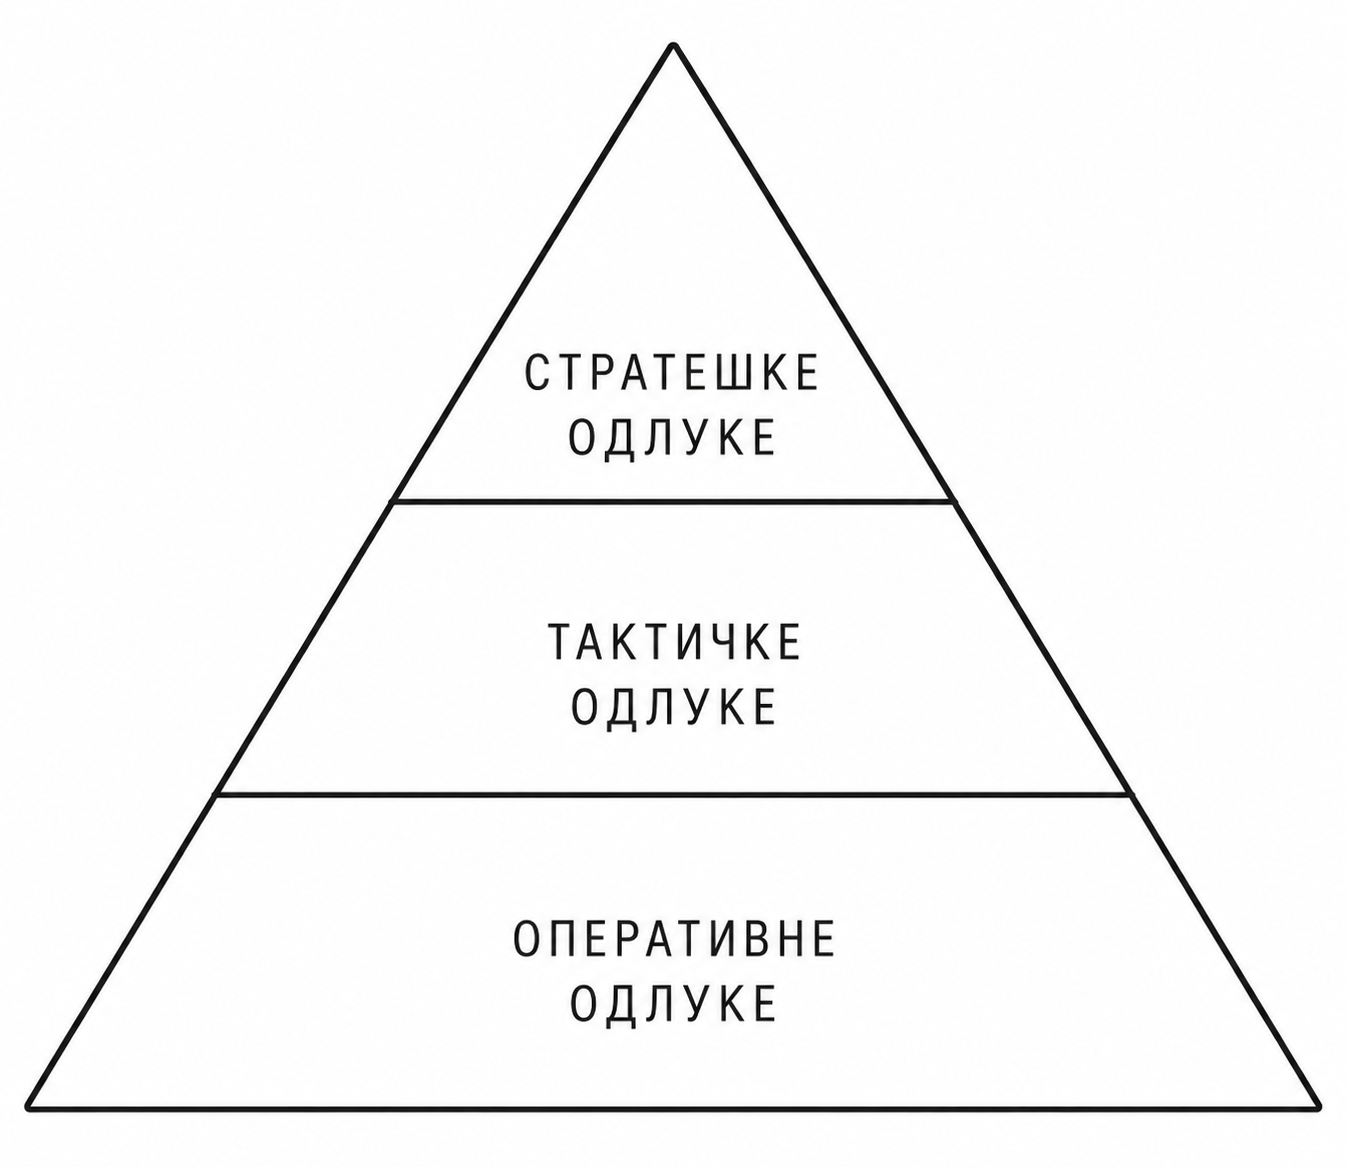
\includegraphics[width=0.85\linewidth]{slike/01/01-09.png}
    \caption{Хијерархија одлука}
    \label{fig:01-1}
\end{figure}

Подршка одлучивању се првенствено користи на стратешком и тактичком нивоу доношења одлука. Пошто су оперативне одлуке устаљене, оне могу да се аутоматизују, те подршка одлучивању код њих није неопходна.

Следи неколико примера у којима се користи подршка одлучивању.

\textbf{Пример 1 (Одлив клијената).}

Компаније све више занима да управљају животним циклусом својих потрошача и да препознају ситуације у којима долази до незадовољства клијента и потенцијалног одласка. Ово се односи на банке, телекомуникационе компаније, али све више и на универзитете који су заинтересовани да уоче ако постоје тешкоће у учењу студената и потенцијалном доношењу одлуке о прекиду студија. Ако се на време препозна намера одласка клијента, може на време и да се предупреди таква одлука.

\textbf{Пример 2 (Хипермаркети).}

Велике продавнице робе широке потрошње желе да сазнају како да што ефикасније управљају својом продајом. Да би то урадили они анализирају узоре продаје артикала како би што боље спознали потрошачке навике и на основу тога доносили одлуке које им могу донети још већу добит.

Проблеме из наведених примера је врло тешко решити без подршке одлучивању и система пословне интелигенције, због захтева за сагледавањем велике количине података, правовременим и исправним одлукама.

Треба напоменути да као што је одлучивање иманентно свим функцијама савременог менаџмента, тако је и подршка одлучивању постала саставни део сваког управљања организацијама заснованог на информационим системима.

\textbf{Подршка одлучивању је интердисциплинарна научна област коју подупире доношење одлуке у различитим менаџмент и бизнис функцијама, као што су маркетинг, финансије, управљање људским ресурсима, управљање производњом, итд.}

\section{Структурираност проблема}
Циљ развоја сваког модела за подршку одлучивању је развити структуриран модел. Тактичке и стратешке одлуке су обично полуструктуриране и неструктуриране. По Сајмону (Херберт А. Сајмон, добитник нобелове награде из економије 1978. године у области истраживања доношења одлуке у организацији), структурираност проблема се може изједначити са његовом дефинисаношћу, а под потпуно дефинисаним (структурираним) проблемом подразумева се да:

1. је проблем јасан,

2. су прецизно дефинисани улазни подаци и

3. су познати начини на који се врши анализа и долази до решења.

Проблеми које је потребно решавати са становишта одлучивања могу бити структурирани, полуструктурирани и неструктурирани. Када је проблем структуриран њега је могуће релативно лако дефинисати, док је за преостала два случаја то значајно теже. У случају неструктурираности ради се о одсуству свих горе наведених елемената, док за полуструктурираност неки од елемената структурираности недостају. Мало аутора се упушта у прецизно дефинисање тих случајева, а ретки су се одлучили да их објасне на свакодневним примерима, као што су то учинили (Leigh \& Doherty, 1986). Због тога се неки њихови примери и наводе у Табели~\ref{tab:01-1}

\begin{table}[h]
\centering
\begin{adjustbox}{max width=\textwidth}
\begin{tabular}{|l|l|l|}
\hline
\textbf{СТРУКТУРИРАНИ ПРОБЛЕМИ} & \textbf{ПОЛУСТРУКТУРИРАНИ ПРОБЛЕМИ} & \textbf{НЕСТРУКТУРИРАНИ ПРОБЛЕМИ} \\
\hline
Открити минус у чековној књижици & Наћи неубележени депозит у књижици & Обезбедити се од таквих проблема у будућности \\
\hline
Возити кола кући & Установити да постоји мали квар на колима & Одржавати кола тако да се не кваре \\
\hline
Израчунати рату за кола & Наћи банку која ће позајмити новац & Постати довољно богат да зајам није потребан \\
\hline
Израчунати цену трансакције са акцијама на берзи & Изабрати групу акција које задовољавају неке критеријуме инвестирања & Тачно предвидети акцију берзе за наредни дан \\
\hline
Попунити кратки формулар & Одредити политику цене за плаћање пореза & Преправити формуларе за плаћање пореза \\
\hline
\end{tabular}
\end{adjustbox}
    \caption{Примери нивоа структурираности проблема}
    \label{tab:01-1}
\end{table}

Занимљиво је да 40 година након објављивања ове табеле, за све од наведених изазова у Табели~\ref{tab:01-1} постоје системи који пружају подршку одлучивању. То су редом: Системи електронског банкарства, Системи превентивног одржавања возила, Електронски инвестициони саветници, Берзански предиктивни системи, Системи за помоћ при попуњавању и преправљање пореских формулара. Оно што је пре 40 година деловало као научна фантастика данас је постала реалност.

Табела~\ref{tab:01-1} представља гледиште поменутих аутора на проблем структурираности. Структурираност се мери у односу на степен знања који ДО поседује о одређеној области. Наиме, ако ДО влада знањем у одређеној области за њега су проблеми из те области структурирани. За ДО ван те области, проблеми су неструктурирани.

Да би ДО могао да решава пословни проблем, он за њега треба да постане структуриран, те је један од основних циљева подршке одлучивања:

\textbf{Превођење проблема одлучивања из неструктурираности у структурираност је неопходан услов за подршку одлучивању, а ово значи да се развије модел за подршку одлучивању.}

Ова једноставна замисао је код решавања реалних проблема прилично сложена. Ипак, од квалитета ове трансформације зависи и процес доношења одлуке.

Надамо се да ће кроз наставак ове књиге постати јасно на које начине може да се изврши ова трансформација и које су предности и недостаци метода које врше овај задатак.

Ако су примери из табеле 1.1. појаснили појам и проблем структурираности остаје да се види зашто је тај проблем интересантан и значајан у подршци одлучивању. Као што је већ напоменуто, у општој теорији одлучивања постоје три врсте одлука: стратешке, тактичке и оперативне. За оперативне одлуке се сматра да су потпуно структуриране, тактичке се крећу од потпуне ка делимичној структурираности, док су стратешке одлуке углавном неструктуриране или у најбољем случају полуструктуриране.

С друге стране, интересантан је однос информационих система, који се користе при одлучивању, према структурираности проблема. Класична обрада података и информациони системи су идеални за проблеме који су потпуно дефинисани (структурирани), док та констатација не важи за преостале случајеве. Како средње и највише руководство (менаџери) доносе тактичке и стратешке одлуке, произилази да су, поготово ови последњи, практично „остали“ без могућности ефикасне рачунарске подршке. Та чињеница је практично и довела до појаве система за подршку одлучивању, као првог „алата“ који се ухватио у коштац са неструктурираним проблемима. (Сукновић и Делибашић, 2010)

\section{Системи за подршку одлучивању}
Први системи који су се формално почели бавити подршком одлучивању као засебном научном дисциплином су системи за подршку одлучивању. Почеци система за подршку одлучивању (СПО) су везани за проучавање одлучивања у организацијама крајем 50-их и почетком 60-их година прошлог века. У седамдесетим годинама 20-ог века је почело и проучавање експертних система (ЕС). СПО и ЕС имају за циљ унапређење пословног одлучивања, а тај циљ остварују различитим приступима.

Најистакнутији аутор из дисциплине СПО (Turban et al., 2006) дефинише СПО преко већег броја дефиниција:

СПО је систем који треба да подржи управљачке одлуке у полуструктурираним и неструктурираним ситуацијама одлучивања.

СПО треба да буде помоћ ДО у смислу повећавања њихових способности, а никако као њихова замена.

СПО је рачунарски систем који пружа подршку при решавању полуструктурираних и неструктурираних проблема у процесу доношења одлука.

СПО пружа адаптиван и еволутивни процес који може помоћи ДО да боље разуме и анализира сопствени процес доношења одлука.

СПО је интерактивни рачунарски систем који користи језике програмирања четврте генерације и базе података за подршку решавању неструктурираних или полуструктурираних проблема у процесу доношења одлука руководства.

СПО су алати, или рачунарски системи који омогућавају бољу продуктивност ДО у процесу одлучивања.

Вишегодишњим изучавањем дисциплине СПО, (Сукновић и Делибашић, 2010) дају следећу дефиницију:

\textbf{СПО су информациони системи, који су слични и комплементарни стандардним информационим системима и имају за циљ да подржавају пословне процесе доношења одлука. Представљају симбиозу информационих система, организационог знања и процеса доношења одлука.}

Већ спомињани (Turban et al., 2006) такође наводи неке од особина СПО које су по њему значајне и које карактеришу сваки СПО:

1. СПО обезбеђује подршку доносиоцима одлука у полуструктурираним и неструктурираним ситуацијама кроз спајање људских процена и рачунарских информација.

2. Подршка је обезбеђена за различите нивое управљања, од највишег ка најнижем.

3. Подршка је обезбеђена како појединцима тако и групама. Шта више, СПО помаже интеграцију појединаца кад год је то потребно.

4. СПО обезбеђује подршку већем броју независних и/или секвенцијалних одлука.

5. СПО подржава све фазе процеса одлучивања: обавештавање, пројектовање, избор и примену (Simon, 1945).

6. СПО подржавају различите процесе одлучивања и различите стилове одлучивања.

7. СПО морају бити адаптивни у времену, а ДО мора бити у стању да реагује на све промене. То омогућава временски адекватне и брзе ad-hoc анализе.

8. СПО треба да буду једноставни за коришћење.

9. СПО треба да побољшају ефективност одлучивања (постизање циљева у посматраном временском периоду), пре него његову ефикасност (оптимизација трошкова одлучивања).

10. ДО има потпуну контролу над свим корацима у процесу одлучивања при решавању проблема. СПО треба да помогну, а не да замене ДО, који увек може да не прихвати сугестију добијену од СПО.

11. СПО треба да води ка учењу, што природно води ка новим унапређењима система, а што опет води ка новом учењу итд.

12. СПО морају бити једноставни за развој, тј. њих треба да могу да конструишу чак и ДО.

Сваки систем за подршку одлучивању се састоји из најмање три подсистема (Sprague \& Carlson, 1982), (Сл. 1.2):

1. Базе података,

2. Базе модела и

3. Корисничког интерфејса.

Подсистем базе података представља део СПО у коме се чувају улазни и излазни подаци организације. Међутим, код база података примењених у СПО постоје и извесне специфичности. Наиме, база података код СПО може да се разликује од релационих база података, о чему ће бити више речи у осталим поглављима ове књиге.

Подсистем базе модела представља компоненту СПО која се састоји од модела одлучивања. Сваки модел решава одређени проблем код одређеног пословног процеса. Њихов задатак је да на основу улазних података и модела одлучивања генеришу излазне податке на основу којих ДО може да доноси одлуке. Улазни, као и излазни подаци могу да се чувају у бази података.

Управљање моделима, као и избор одговарајућег модела, је код класичних СПО препуштен ДО. Типични модели који се налазе у бази модела СПО служе подршци решавању полуструктурираних и неструктурираних проблема одлучивања.

По поменутим ауторима кључне особине СПО у подсистему модела укључују способности:

1. укључивања нових модела у систем,

2. приступања и интеграцији „блоковима модела“ ради добијања новог модела,

3. каталогизирања и одржавања широког опсега модела за различите кориснике,

4. повезивања ових модела са одговарајућим везама у бази података и

5. управљања базом модела.

Подсистем корисничког интерфејса по својој основној функцији треба да омогући (и то на што једноставнији начин) комуникацију између СПО и корисника. То је управо због ДО, који по правилу нису специјалисти за одређени модел, основни разлог због чега је овај подсистем и најважнији. СПО могу да користе како крајњи ДО, тако и аналитичари који припремају одлуке користећи СПО за ДО.

\begin{figure}[h]
    \centering
    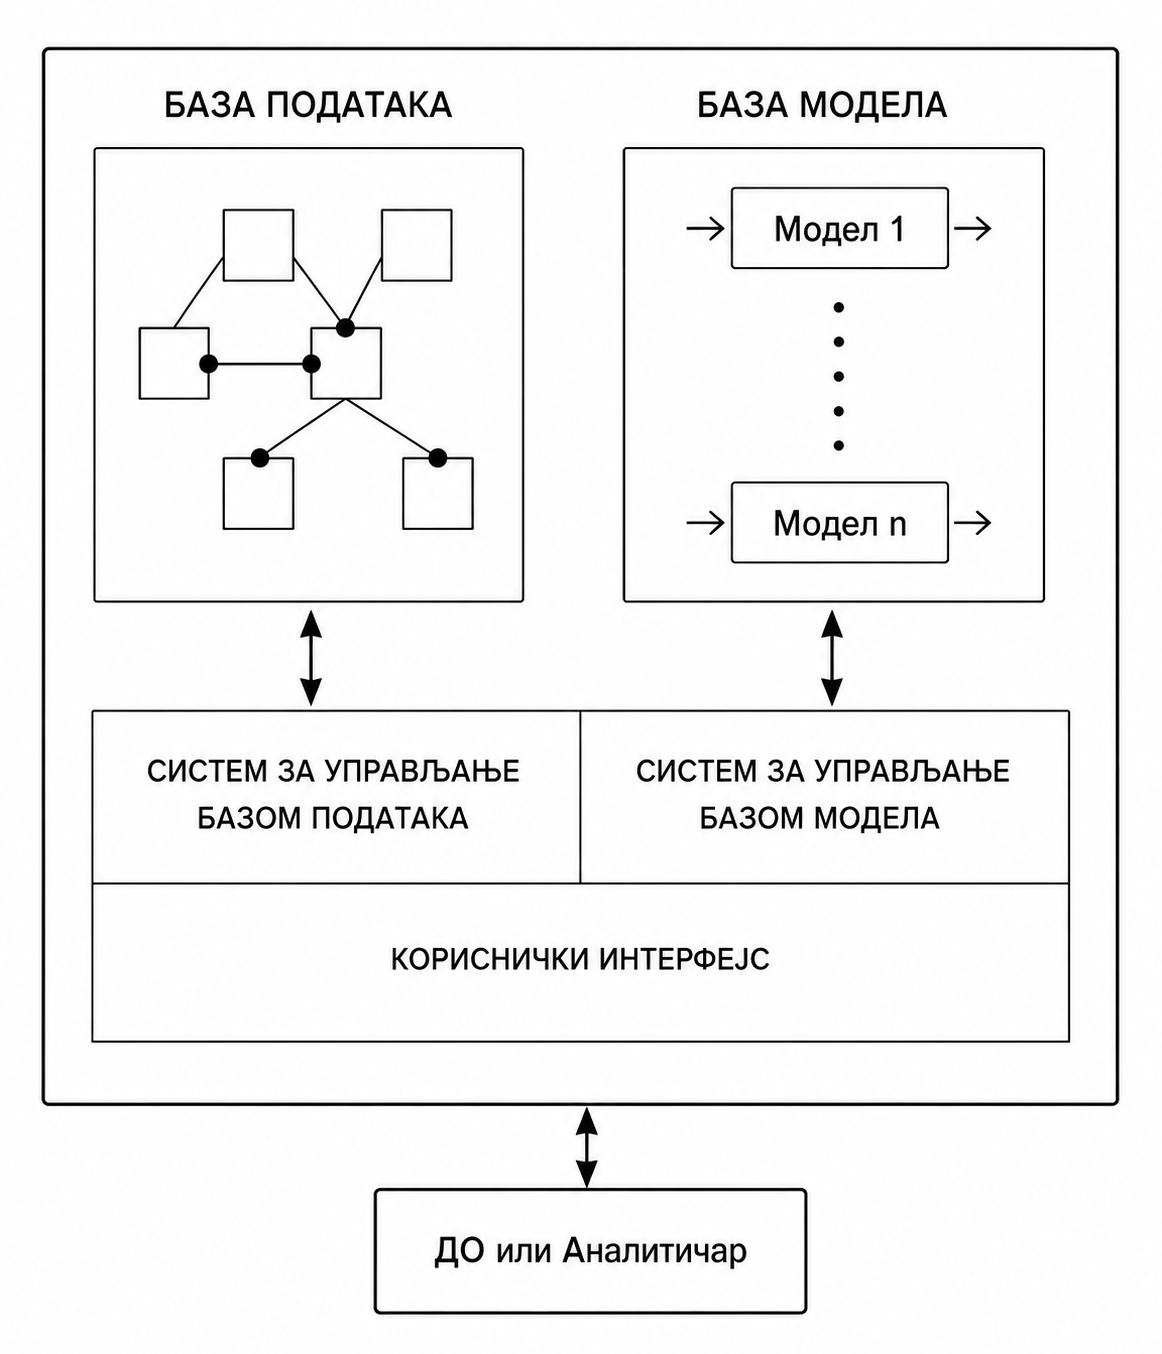
\includegraphics[width=0.85\linewidth]{slike/01/01-30.png}
    \caption{Компоненте СПО}
    \label{fig:01-2}
\end{figure}

У већини случајева се подсистем корисничког интерфејса састоји из три дела (Bennett, 1983):

1. језик акције: којим корисник комуницира са системом,

2. језик презентације: шта корисник види на интерфејсу и

3. база знања: шта корисник мора знати (о систему за подршку одлучивању).

(Turban et al., 2006) наводи сличну структуру архитектуре СПО и сматра да се сваки СПО састоји из следеће три компоненте:

1. Управљање подацима - укључује базе података са релевантним подацима за посматрану ситуацију и управљане софтвером, који се зове систем за управљање базом података (СУБП);

2. Управљање моделима - софтверски пакет, који укључује финансијске, статистичке, управљачке и друге квантитативне моделе и који систему даје аналитичке могућности као и одговарајуће управљање софтвером;

3. Комуникацијски подсистем (кориснички интерфејс) - преко кога корисник комуницира са СПО и управља њиме.

СПО нуди одређене предности када се уведе у организацију. Основне предности СПО, које је још давне 1981. године навео (Keen, 1981) су:

1. Повећавање броја алтернатива за разматрање у процесу доношења одлука;

2. Боље разумевање проблема који треба да се реши;

3. Бржи одговор на непредвиђене ситуације; тј. краће време потребно за доношење полуструктурираних и неструктурираних одлука;

4. Способност спровођења ad-hoc анализа;

5. Боље сагледавање проблема и учење;

6. Побољшана комуникација међу члановима тима који учествују у доношењу одлуке;

7. Побољшана контрола одлучивања;

8. Уштеда у трошковима;

9. Боље одлуке;

10. Ефикаснији тимски рад;

11. Уштеда у времену и

12. Боље искоришћење расположивих података.

Са друге стране, класични СПО имају и одређене недостатке којих сваки инжењер који уводи овај систем у организацијама треба да буде свестан. Недостаци који се наводе у наставку су само делимично решени, те су неки од њих и данас актуелни.

Основни недостатак СПО огледа се у чињеници да постоји проблем избора и коришћења модела из базе модела. Наиме, када СПО има само један модел, овај проблем не постоји, али најчешће то није случај. СПО, по правилу, увек на располагање ДО нуде више различитих модела за решавање истог проблема. ДО тада може да има недоумицу:

1. Који модел изабрати?

2. Како користити изабрани модел? (иако ово зависи од способности и вештине ДО, постоје захтеви да се постојећи модел унутар СПО приближи ДО који решава реалне проблеме. Најчешће је потребно прилагодити постојеће моделе и то је процес који отежава примену СПО).

3. Како решити проблем за чије решавање не постоји модел у бази модела?

Сматра се да се проблем управљања базом модела може решити коришћењем експертног система (потпоглавље 1.5). У сваком случају је потребно експертско знање за решавање напред набројаних недоумица. У наставку књиге биће предложена могућа решења.

Иако је СПО технологија деведесетих година 20. века достигла свој зенит, може да се каже да је наставила да се развија под другим називима. Наследник СПО је свакако ПИ, али су се упоредо развијали и други системи, пре свега системи вештачке интелигенције (ВИ) и машинског учења (МУ) (Делибашић и други, 2009), који су постали доминантни у пружању подршке одлучивању.

За обраду података код СПО, за разлику од класичне обраде података, неопходне су могућности спровођења „шта-ако“ анализе, анализе осетљивости и анализе достизања циља. Ове анализе су изузетно значајне у процесу доношења одлука.

Да би се појаснило место СПО у рачунарским и информационим наукама даје се преглед технологија које се користе за подршку одлучивању:

\begin{itemize}
  \item Управљање ресурсима предузећа – ЕРП (енг. Enterprise Resource Planning): информациони системи који подржавају трансакциону обраду података, прикупљају и складиште трансакционе податке организација и омогућавају процесну интеграцију података.
  \item Пословна интелигенција – ПИ: информациони системи који подржавају аналитичку обраду података, подаци из ЕРП система су пречишћени, интегрисани, и спремни за анализу. Корисницима су на располагању контролне табле, аналитичке коцке, пивот табеле, којима могу да навигирају кроз податке организације и праве, између осталог, и ad-hoc упите.
  \item Системи за подршку одлучивању – СПО: информациони системи који уводе додатне аналитичке капацитете са циљем да се подржи процес одлучивања. Уводи се димензија акција за одлучивања, које нису експлицитно биле изражене код ЕРП и ПИ. Подржавају се предиктивна аналитика, анализе осетљивости, противчињеничне анализе, моделовање сценарија, оптимизационе процедуре. Да би се испунили сви ови аналитички и одлучивачки захтеви користе се, између осталих, и методе ВИ и МУ.
\end{itemize}
Да би се предвидело како ће будућност система пословне интелигенције изгледати, треба се сетити генеричког оквира за развој СПО предложеног од стране (Holsapple \& Whinston, 1996), а приказаног на слици 1.4. Овај оквир пружа прилично стабилан поглед на технологију СПО, шта она представља и шта ће представљати и у времену које долази.

\begin{figure}[h]
    \centering
    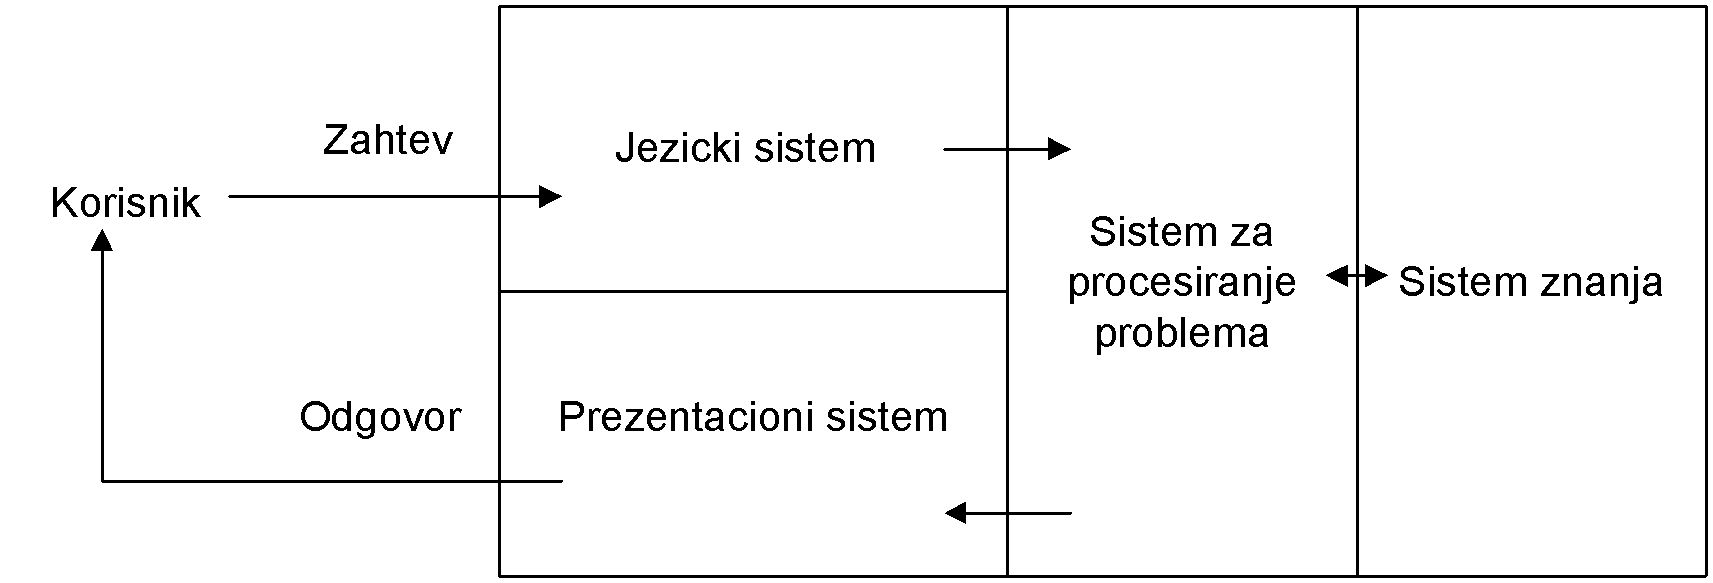
\includegraphics[width=0.85\linewidth]{slike/01/01-26.png}
    \caption{Генерички оквир СПО}
    \label{fig:01-3}
\end{figure}

Генерички оквир за развој СПО треба да омогући ефикасну комуникацију између ДО и података организације. Да би ДО из података добио одговарајућу подршку одлучивању најпре треба да има могућност да преко одговарајућег интерфејса (језички систем) пренесе свој захтев (дефинисан проблем) систему.

Након примљеног захтева систем треба да анализира проблем (систем за процесирање проблема). СПО на основу знања садржаног у систему и захтева корисника треба да генерише одговарајући одговор (предлог решења). Одговор кориснику на постављени захтев СПО омогућава преко презентационог система.

Већина СПО се и развија да садржи све компоненте система, међутим овакво гледање на СПО нам омогућава да посматрамо СПО као технологију која се може придодати свим организационим системима и тиме повећати квалитет доношења одлука.

\textbf{Као што је одлучивање иманентно свим функцијама организације, тако је и подршка одлучивању иманентна свим системима развијеним да подрже одлучивање у свим функцијама организације.}

Један поглед како би СПО могли да изгледају предложили су и (Azvine et al., 2006). Аутори описују како би СПО могао изгледати у будућности. СПО би, по наведеним ауторима, требало да задовољи следеће услове:

\begin{itemize}
  \item пуњење података у базу података у реалном времену,
  \item пуњење модела из базе модела у реалном времену,
  \item анализа резултата модела у реалном времену и
  \item доношење одлуке у реалном времену.
\end{itemize}
Да се СПО мењају потврђује и (Lawton, 2006), који наводи да је кориснички интерфејс система ПИ знатно побољшан у односу на претходни период, а неке апликације ПИ већ омогућавају рад у реалном времену.

Визија савремених система СПО је да се омогући функционисање система који ће омогућити пут од захтева за решењем до решења (информације са предлогом одлуке) без застоја и препрека, тј. у реалном времену. Да би се то постигло, процес доласка до знања (информација са предложеном акцијом одлуке) треба да се аутоматизује.

\textit{Данас, захваљујући напретку у облаку рачунарства (енг. Cloud Computing), платформама за обраду великих података (нпр. Apache Hadoop, Apache Spark) и самоуслужним БИ алатима (нпр. Power BI, Tableau, Looker), овај циљ је у значајној мери остварен. Савремени системи ПИ омогућавају корисницима да сами креирају извештаје и визуализације без потребе за специјализованим аналитичарима, чиме се драстично скраћује време од податка до одлуке. Додатно, примена машинског учења и вештачке интелигенције (укључујући и велике језичке моделе) аутоматизује многе кораке у аналитичком процесу.}

У наставку се приказују слојеви који чине структуру једног интегрисаног система пословне интелигенције (Слика~\ref{fig:01-4}). То су:

1. трансакциони (оперативни),

2. интегративни и

3. аналитички слој.

\begin{figure}[h]
    \centering
    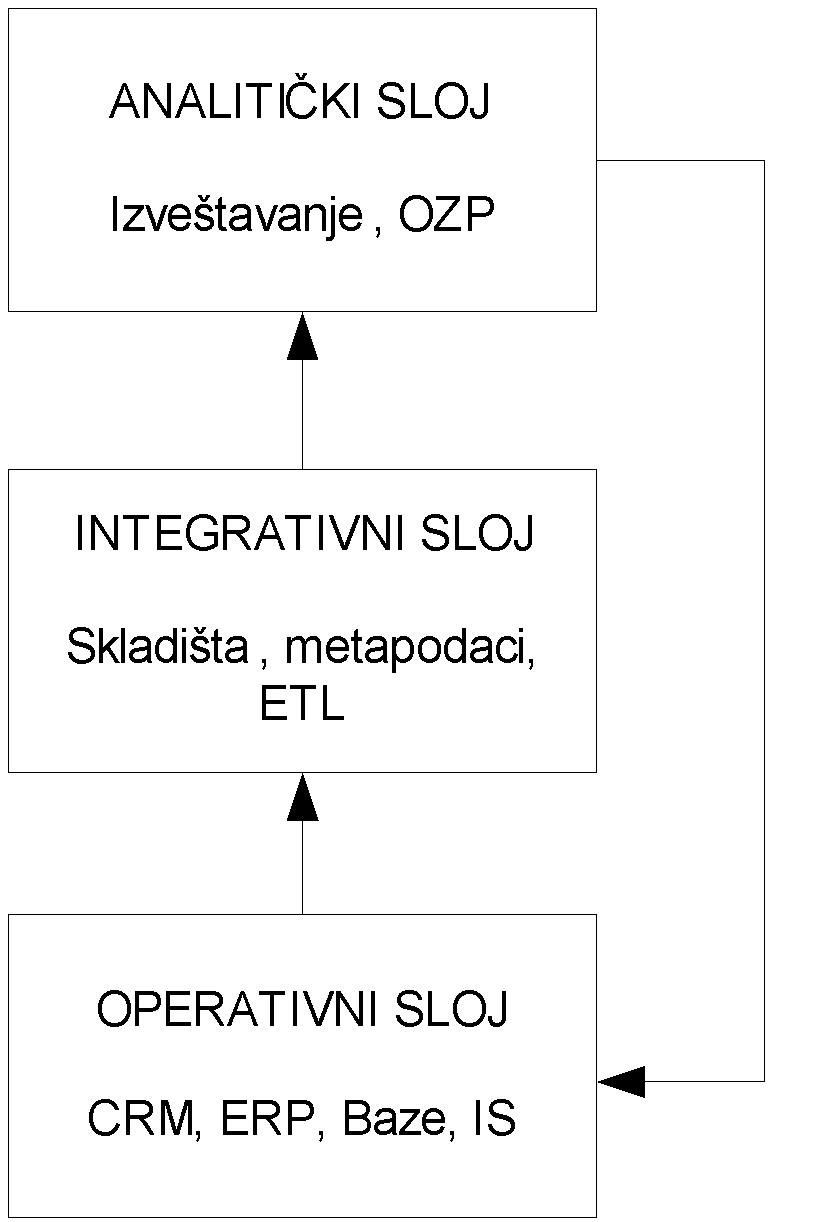
\includegraphics[width=0.85\linewidth]{slike/01/01-28.png}
    \caption{Три слоја пословне интелигенције}
    \label{fig:01-4}
\end{figure}

Трансакциони или оперативни слој генерише податке пословања. Систем ПИ треба да буде везан за овај слој, и то двоструко. Све што се дешава у текућем пословању организације треба да се очитава у складишту података, и са друге стране: одлуке донете на основу извештаја из аналитичког слоја треба да се одразе у оперативном слоју и повратно кроз сам систем ПИ. Да би ово било могуће потребно је укључити следеће функционалности у систем ПИ:

1. Организациони (пословни) процеси треба да буду снимани константно и подаци из тог процеса учитавани у складиште података и

2. одлуке које доноси ДО треба да утичу на сам пословни процес.

Други важан слој система ПИ јесте интегративни слој. Овај слој представља спону између модела и података пословања. Он треба да обезбеди квалитетне податке за аналитички слој. Да би овај слој функционисао у реалном времену треба да се омогући:

1. Једноставан приступ подацима пословања кроз дефинисано складиште података (тема поглавља 2),

2. дефинисан ток учитавања података из пословања у складиште података и

3. систем за управљање квалитетом података и решавање проблема неквалитетних података код процеса учитавања података у складиште.

Аналитички слој је одговоран за прављење извештаја за ДО, у њега су укључени алати за извештавање као и различити модели из базе модела (међу њима највише се истичу алгоритми за откривање законитости у подацима – ОЗП) чији је задатак да на основу захтева корисника и података из базе података реше захтев ДО.

Пошто су модели на основу којих се праве извештаји и даље прилично сложени, овај слој у великој мери зависи од способности аналитичара коме је, са друге стране, потребна одређена количина времена док састави извештај или примени одговарајући модел. Аналитичар због сложености свог посла често је био уско грло интегрисаног система пословне интелигенције, тј. време које је њему/њој било потребно да састави одређени извештај имало је директни утицај на време које је потребно да се ДО пружи подршка одлучивању.

Да би систем ПИ могао да функционише у реалном времену, потребно је знања аналитичара, тј. његова експертска знања, формализовати и аутоматизовати. Знање аналитичара је било потребно аутоматизовати да би се омогућио аутоматски избор модела као и њихова примена. У данашње време, развојем великих језичких модела и агентских модела ово се све више постиже тако што се аутоматски бирају и подешавају модели за одређени скуп података.

Избор одговарајућег модела треба да зависи од природе корисничког захтева и од података који стоје на располагању за решавање тог захтева. Аналитичар у систему будућности добија нову улогу. Он треба да изврши почетно подешавање параметара система и да током функционисања система врши промену параметара и адаптацију система током времена.

\begin{figure}[h]
    \centering
    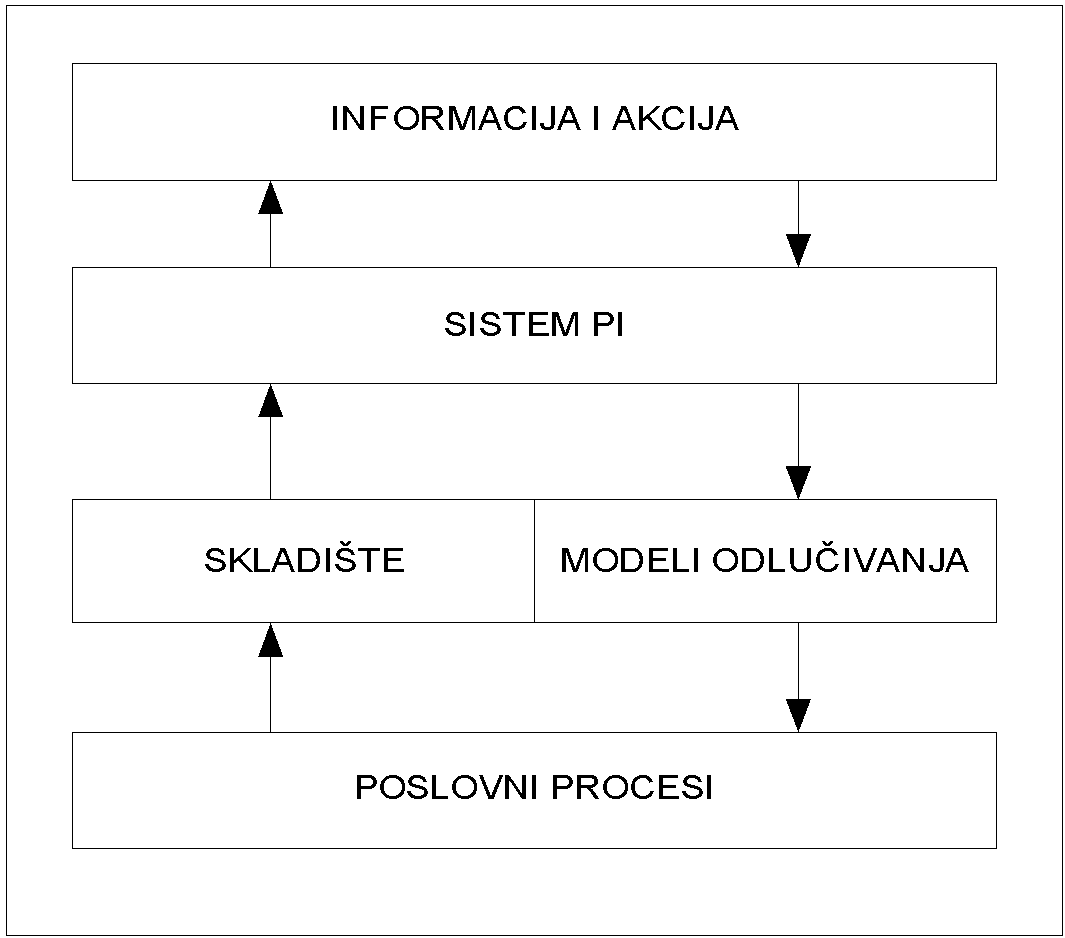
\includegraphics[width=0.85\linewidth]{slike/01/01-20.png}
    \caption{Систем пословне интелигенције у реалном времену}
    \label{fig:01-5}
\end{figure}

\section{Експертни системи}
Као алати који треба да симулирају знање експерта, експертни системи (ЕС) могу да се дефинишу као програми који користе људско знање ради решавања проблема који захтевају људску интелигенцију. Једна од најпотпунијих дефиниција за ЕС потиче од врсног познаваоца ове области, Едварда Фајгенбаума (са Универзитета Стенфорд (Stanford)):

\textbf{Експертни системи су интелигентни рачунарски програми који употребљавају знање и процедуре закључивања да би решили проблеме који су довољно тешки, те захтевају значајну људску стручност и вештину. Знање са додатком механизма закључивања за решавање тог проблема могу се сматрати моделом који симулира најбољег стручњака у тој области.}

Да би се решили сложени полуструктурирани и неструктурирани проблеми потребно је експертско знање. Један од поменутих сложених проблема јесте проблем избора и примене одговарајућег модела, поменутог као један од изазова код традиционалних СПО. Како је подршка одлучивања скупа, а неопходна, развијани су експертни системи са циљем да симулирају знање врхунског експерта, које је са друге стране, било потребно за решавање пословних проблема.

\textit{Напомена: Класични експертни системи засновани на правилима (енг. Rule-based expert systems) су данас у значајној мери замењени или допуњени системима машинског учења који аутоматски уче обрасце из података, или великим језичким моделима који управо симулирају знање врхунског експерта. Разумевање принципа експертних система је важно јер је то темељ на коме су настали савремени системи вештачке интелигенције, а њихови елементи се и даље се користе при решавању реалних проблема.}

\subsection{Архитектура експертног система}
Сваки ЕС се састоји из три основна дела (Слика~\ref{fig:01-6}). То су:

\begin{itemize}
  \item база знања,
  \item механизам закључивања и
  \item кориснички интерфејс.
\end{itemize}

\begin{figure}[h]
    \centering
    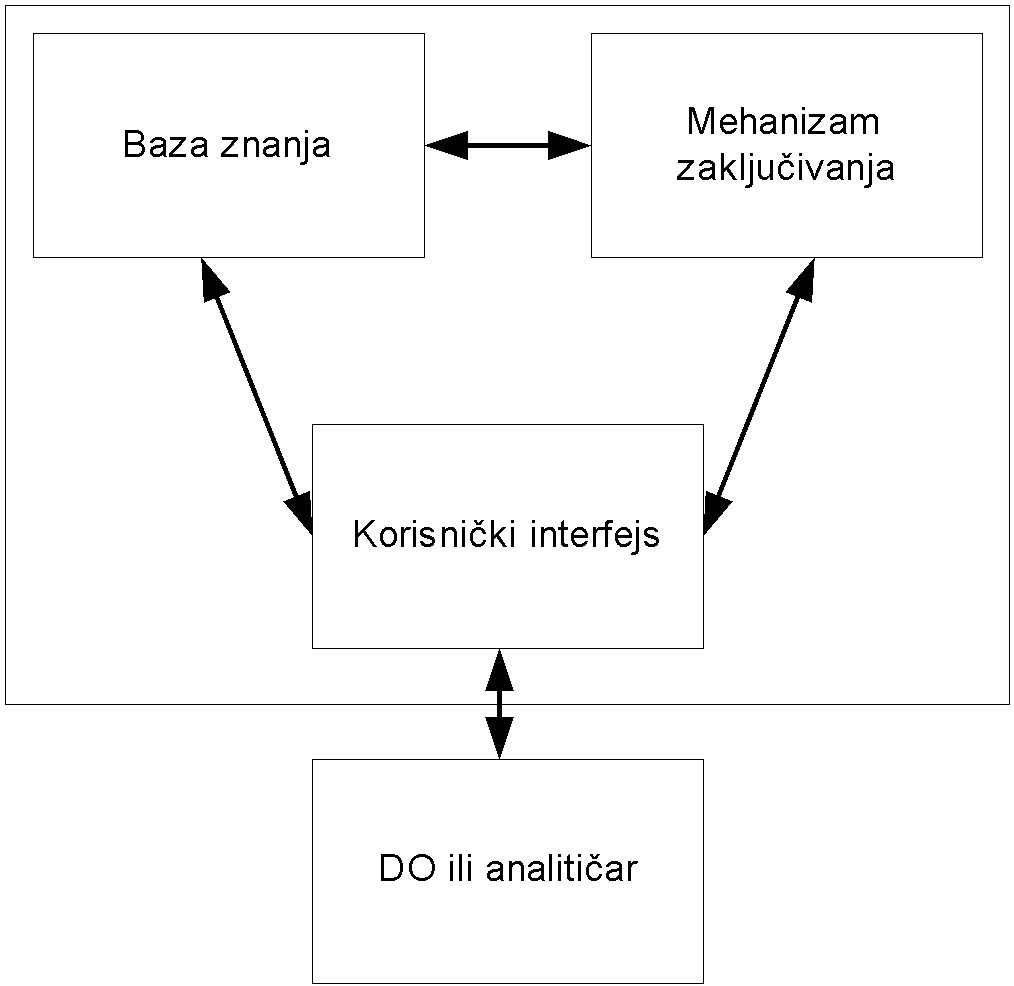
\includegraphics[width=0.85\linewidth]{slike/01/01-22.png}
    \caption{Основна архитектура експертног система}
    \label{fig:01-6}
\end{figure}

База знања садржи знање експерта у рачунски читљивом формату.

Механизам закључивања има за циљ да на основу захтева корисника и знања у бази знања реши кориснички захтев, тј. да пронађе управо оно знање које је кориснику потребно. Механизам закључивања има две основне улоге:

1. испитује постојање одређеног знања у бази знања на основу корисничког захтева и проналази неопходно знање за решавање корисничког захтева и

2. уређују редослед кретања по бази знања у зависности од захтева корисника и структуре базе знања. Ово може бити и интерактиван процес.

Кориснички интерфејс треба да обезбеди једноставну комуникацију између система и корисника, тако што треба да омогући једноставну управљање експертним системом и квалитетну интерпретацију резултата.

\subsection{База знања}
База знања представља критични део експертног система. Због тога је поступак прикупљања знања од експерта, трансформација експертског знања у формални облик и организација базе знања најбитнији процес развоја експертног система.

База знања садржи законитости из специфичног домена знања које се моделирају. Постоје различити начини да се знање запише у читљивом облику за машине. Најпознатије методе представљања знања у бази знања су:

\begin{itemize}
  \item продукциона (ако-тада) правила,
  \item семантичке мреже,
  \item оквири знања,
  \item математичка (формална) логика,
  \item табеле одлучивања,
  \item дрво одлучивања, итд.
\end{itemize}
\textbf{Продукциона правила}

Представљају најчешће коришћени метод представљања знања. То су правила облика АКО услов ТАДА последица. Продукционим правилима се представљају логичке релације (везе) међу подацима. Овакав начин представљања знања је доста природан, а што је врло важно, има особину модуларности. Такође, задовољавају захтев за лаком модификацијом базе знања.

\begin{figure}[h]
    \centering
    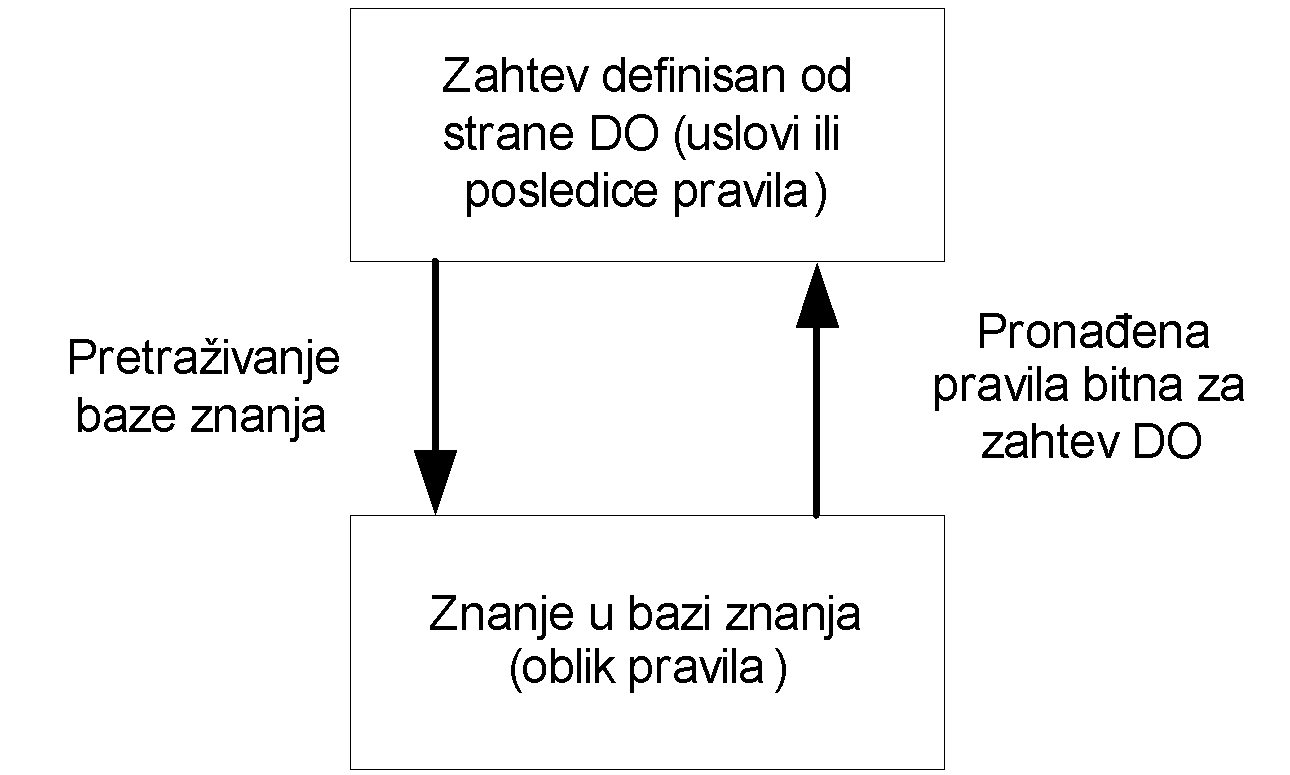
\includegraphics[width=0.85\linewidth]{slike/01/01-33.png}
    \caption{Однос правила и знања у радној меморији}
    \label{fig:01-7}
\end{figure}

\textbf{Семантичке мреже}

Знање представљају у облику мреже. Свака мрежа се састоји од чворова и веза међу чворовима. Везе исказују односе међу чворовима. Везе могу да приказују и наслеђивање међу чворовима.

\begin{figure}[h]
    \centering
    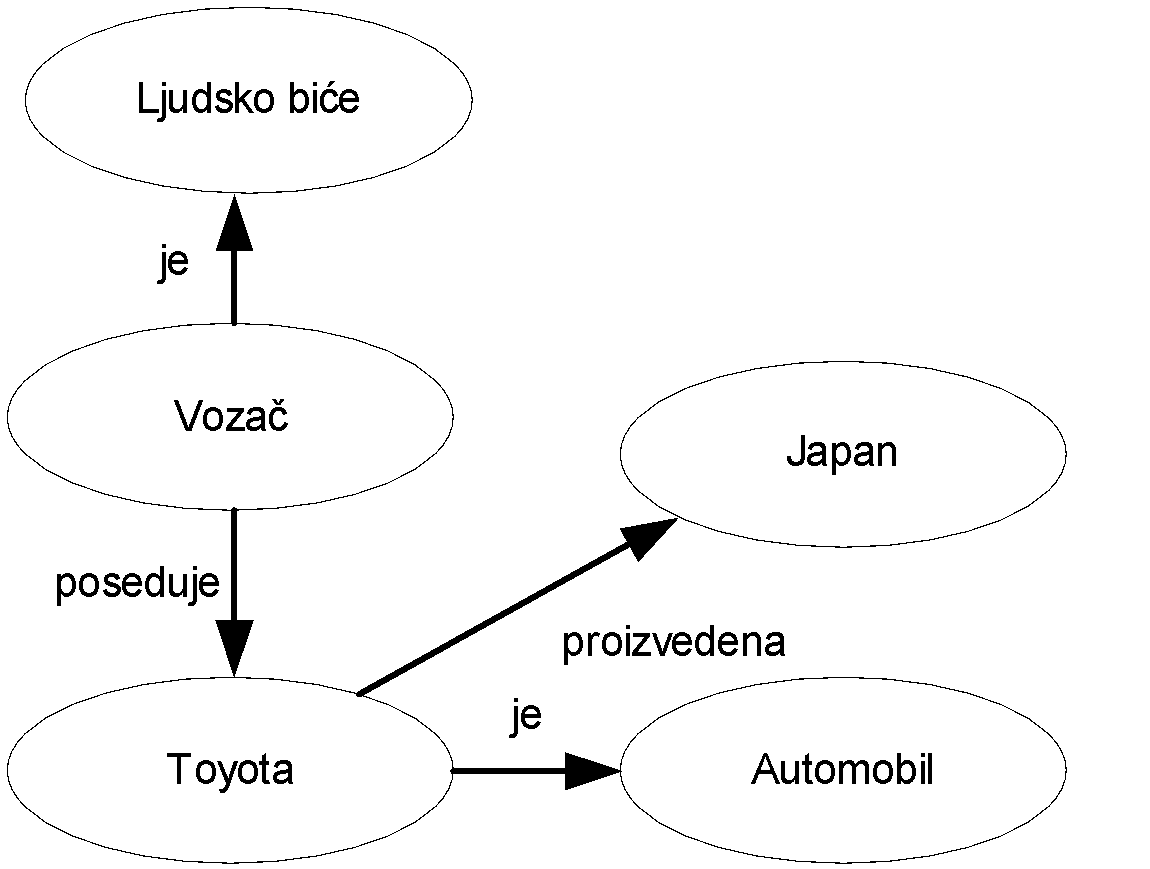
\includegraphics[width=0.85\linewidth]{slike/01/01-31.png}
    \caption{Пример семантичке мреже}
    \label{fig:01-8}
\end{figure}

\textbf{Оквири знања}

Представљају скупове објеката, који се састоје од атрибута, где сваки атрибут има одређену вредност. Оквири знања представљају специјалан случај семантичких мрежа. Сваки оквир има статички део (подаци исти за класу објеката) и динамички део (подаци карактеристични за одређени објекат).

\begin{figure}[h]
    \centering
    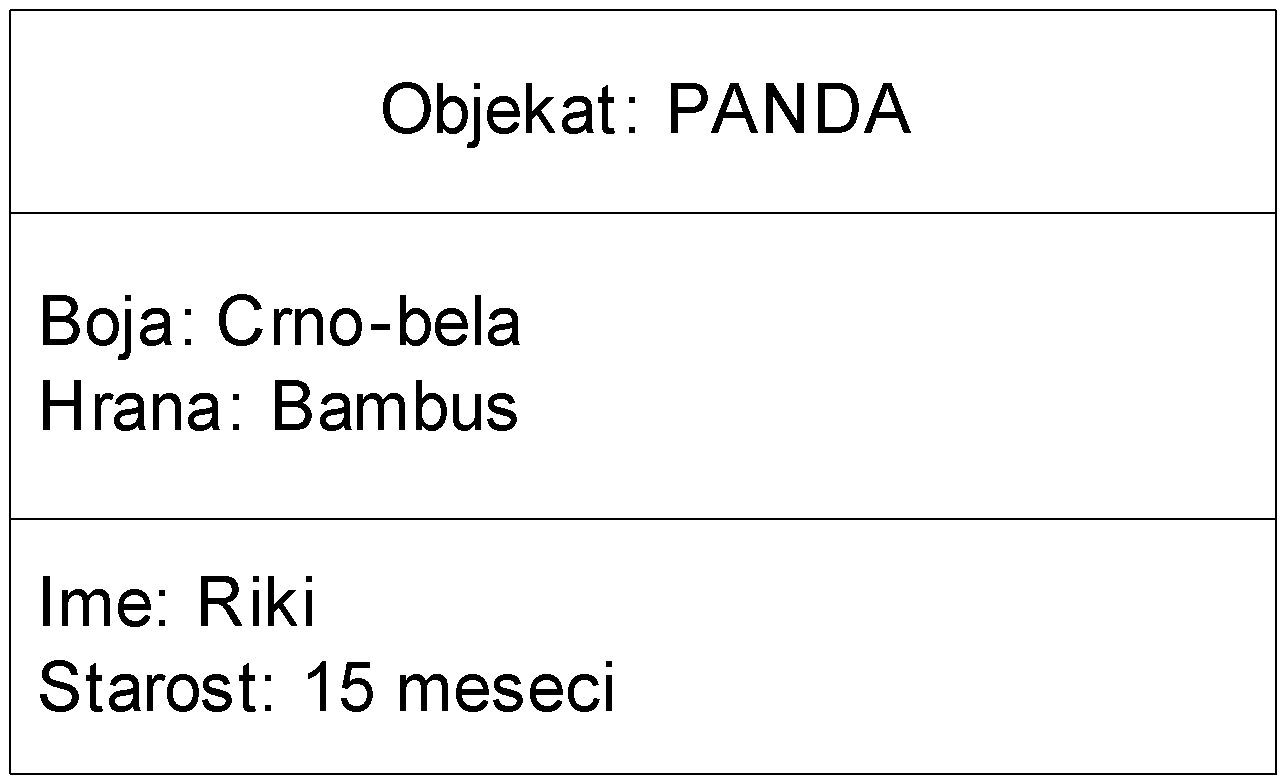
\includegraphics[width=0.85\linewidth]{slike/01/01-12.png}
    \caption{Пример оквира знања}
    \label{fig:01-9}
\end{figure}

\textbf{Математичка (формална) логика}

Код представљања знања математичком логиком, користе се најчешће две врсте логика: пропозициона логика и предикатски рачун. Пропозициона логика представља систем за закључивање у коме испитује да ли је одређена премиса тачна или није. Предикатски рачун представља проширење пропозиционе логике.

\textbf{Табела одлучивања}

Табела одлучивања представља још један вид чувања знања. Табела се састоји од атрибута и редова, а неки од атрибута могу садржати акцију одлучивања. Ове табеле представљају основни облик из којих алгоритми машинског учења развијају моделе, који даље могу да се употребљавају како у ЕС, тако и у другим СПО. Табела може да чува у себи или правила одлучивања или случајеве претходног искуства који су довели до одређене одлуке.

\begin{table}[h]
\centering
\begin{adjustbox}{max width=\textwidth}
\begin{tabular}{|l|l|l|l|l|l|}
\hline
\textbf{Дан} & \textbf{врем. прилике} & \textbf{температура} & \textbf{влажност} & \textbf{ветар} & \textbf{играти?} \\
\hline
1 & сунчано & Вруће & висока & слаб & не \\
\hline
2 & сунчано & Вруће & висока & јак & не \\
\hline
3 & облачно & Вруће & висока & слаб & да \\
\hline
4 & кишовито & Топло & висока & слаб & да \\
\hline
5 & кишовито & Хладно & нормална & слаб & да \\
\hline
\end{tabular}
\end{adjustbox}
    \caption{Скуп случајева одигравања утакмица за голф}
    \label{tab:01-2}
\end{table}

\textbf{Стабло одлучивања}

Стабло одлучивања чува знање у хијерархијском облику који је једноставно читљив. Оно може бити индуковано алгоритмима машинског учења из табела одлучивања, али исто тако може бити моделовано од стране експерта.

\begin{figure}[h]
    \centering
    
\includegraphics[width=0.85\linewidth]{slike/01/01-34.png}
    \caption{Стабло одлучивања за играње голфа}
    \label{fig:01-10}
\end{figure}

Овим свакако није исцрпљен преглед метода за чување знања. Треба имати на уму да се у решавању практичних проблема најчешће комбинује више различитих метода за представљање знања.

Без обзира на изабрани начин представљања знања, прикупљање истог је важна компонента приликом развијања експертног система. Овај посао поверен је такозваном инжењеру знања (\textit{knowledge engineer}), чији је задатак да успостави контакт са експертом и да запише знање експерта. Сам процес прикупљања знања од експерата назива се аквизиција знања (\textit{knowledge acquisition}).

\subsection{Механизам закључивања}
Представља део ЕС који има задатак да пронађе одговарајуће знање у бази знања и да га примени за решавање проблема. Захваљујући овом процесу каже се да су ЕС програми који се понашају „интелигентно“. Без механизма закључивања ЕС би био само енциклопедија, док је са механизмом закључивања ЕС деловао, у тадашње време, сличнији људском резоновању. Два су приступа у имплементацији механизама закључивања, и то: уланчавање унапред и уланчавање уназад.

\textbf{Уланчавање унапред}

Уланчавање унапред полази од премиса, АКО делова правила, у бази знања и упоређује их са чињеницама у меморији које је корисник изнео. Правила која су задовољена, могу се реализовати тако да се њихови ТАДА делови изврше. Ако се приликом претраживања покаже да ни једно правило није задовољено, ЕС закључује да нема довољно података да би проблем могао да се реши.

\textbf{Уланчавање уназад}

Уланчавање уназад је поступак обрнут од поступка уланчавања унапред. Код њега се полази од закључка, од ТАДА делова правила. Прво се претпостави да неко од могућих решења проблема важи и оно се означи као текућа хипотеза. Затим се проверава да ли важе све премисе тог правила. Овај поступак се рекурзивно понавља док год траје интеракција са корисником или док нема више правила у бази знања.

\subsection{Кориснички интерфејс}
Трећа, али подједнако значајна, компонента код ЕС је кориснички интерфејс. Основна улога овог елемента је да омогући рад корисника са експертним системом.

Поред дизајна, који је значајан за коришћење ове компоненте, изузетно је битно да корисник може:

1. јасно да изнесе свој кориснички захтев и

2. јасно да разуме резултате које му враћа систем.

Након представљања две различите технологије за подршку одлучивању, СПО и ЕС, следи потпоглавље о могућности комбиновања ова два приступа.

\section{Интеграција СПО и ЕС}
Успешна интеграција СПО и ЕС представља додатно побољшање оба приступа, у односу на ситуације када се они користе појединачно. Интеграцију ЕС и СПО је теоријски, а у неким случајевима и практично, могуће извести на пет различитих начина.

По (Turban \& Carlson, 1989) могуће комбинације „прикључења“ експертних система на системе за подршку одлучивању, се могу свести на неке типичне случајеве приказане на слици 1.13.

1. ЕС\#1 и ЕС\#2 уносе елементе интелигенције у системе за управљање базама података и модела, што је посебно значајно у овом другом случају.

2. ЕС\#3 има за циљ помоћ при коришћењу корисничког интерфејса.

3. ЕС\#4 и ЕС\#5 су замишљени као консултантска помоћ како градитељима СПО тако и њиховим корисницима.

\begin{figure}[h]
    \centering
    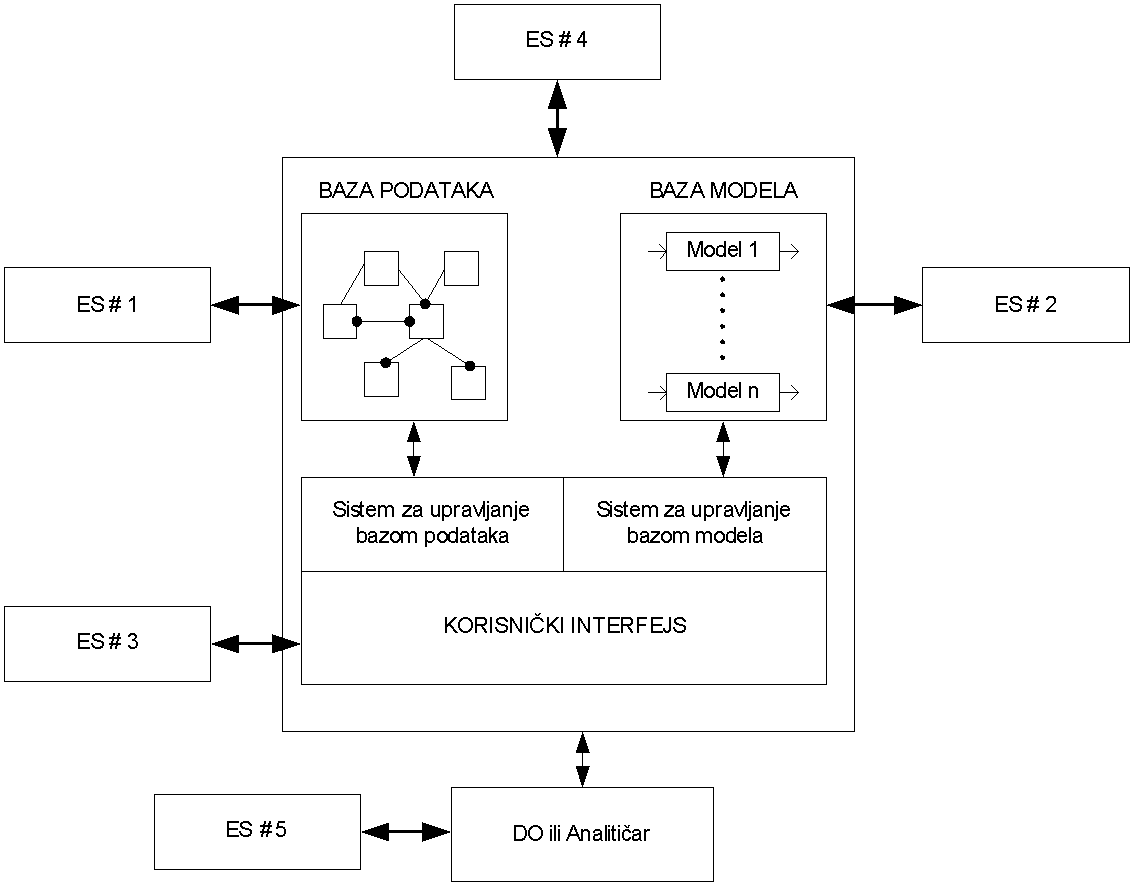
\includegraphics[width=0.85\linewidth]{slike/01/01-13.png}
    \caption{Могућности прикључења ЕС на СПО}
    \label{fig:01-11}
\end{figure}

Сви наведени начини прикључења решавају неки значајан проблем код развоја или коришћења СПО. Данас се све више, уместо ЕС, користе и друге технологије за решавање истих проблема. Пре свега се мисли на откривање законитости у подацима (ОЗП), велике језичке моделе и агентске системе.

По (Turban \& Carlson, 1989) ЕС је могуће придодати и као посебну компоненту СПО. Развијено је неколико могућности:

1. Излаз ЕС као улаз у СПО: Овај приступ је нарочито интересантан за почетне фазе процеса одлучивања.

2. Излаз СПО као улаз у ЕС: Овај приступ је посебно популаран јер експертним системима омогућује коришћење резултата различитих квантитативних анализа.

3. Повратна спрега: Представља комбинацију прва два приступа.

(Meader et al., 1984) су пошли од анализе процеса одлучивања и закључили да је већину уобичајених корака у том процесу могуће подржати типичним СПО функцијама. За кораке који подразумевају коришћење процена и креативности, они предлажу употребу ЕС.

(Roland, 1982) је уочио да ће СПО тешко моћи да доносиоцу одлуке сугеришу алтернативне акције које треба разматрати при одлучивању (фаза пројектовања по Сајмону), док ће бити у стању да кориснику помогну при евалуацији и избору између потенцијалних акција (фаза избора при одлучивању). Са степеном развоја данашњих технологија, ово више није немогуће, већ врло извесно.

До сада су разматрани системи за подршку одлучивању и експертни системи који превасходно подржавају индивидуално доношење одлука. Међутим, као што је већ напоменуто у особинама СПО (особина 3), подршка одлучивању није ограничена само на појединца – она треба да подржи и групно доношење одлука. У савременим организацијама, већину сложених одлука доносе групе људи, које су све чешће просторно и временски раздвојени. Из тог разлога, развијени су специјализовани системи који проширују концепт индивидуалног СПО на групни контекст. У наредним потпоглављима биће представљени алати за подршку рада групе и групни системи за подршку одлучивању (ГСПО), који омогућавају ефикасно колаборативно доношење одлука.

\section{Проблем базе модела код СПО}
Експертни системи поред основне намене, чување знања експерата, имају још неколико важних особина када се посматрају у односу на СПО (Сукновић и Делибашић, 2011):

1. Интеграцијом ЕС у СПО значајно се побољшава проблем управљања базом модела СПО.

2. Успешно реализована интеграција ЕС и СПО, представља први корак у креирању нових врста информационих система као што су: Информациони системи за извршне руководиоце (Executive Information Systems), Системи за подршку извршних руководиоца (Executive support systems), Системи за подршку менаџменту (Management support systems), итд.

Први који су у терминологију СПО увели појам базе модела су били (Sprague \& Carlson, 1982). Они су тада правилно уочили да процес креирања модела мора бити флексибилан, обављен са формалним језицима за моделирање и скупом „блокова за градњу“, који подсећају на потпрограме које је могуће склопити у циљу процеса моделирања.

У реализацији такве жеље није постигнут очекивани резултат. По мишљењу аутора ове књиге исувише истраживачког времена је изгубљено у покушају да се прекопира концепт управљања базама података на управљање базама модела. Данас је очигледно, да се радило о практично немогућем задатку, због фундаменталне разлике између података и модела.

Многи аутори су се бавили проблематиком управљања моделима. (Turban et al., 2006) је дао вероватно најпотпунији приказ оног што се под управљањем моделима подразумева (Слика~\ref{fig:01-12}).

\begin{figure}[h]
    \centering
    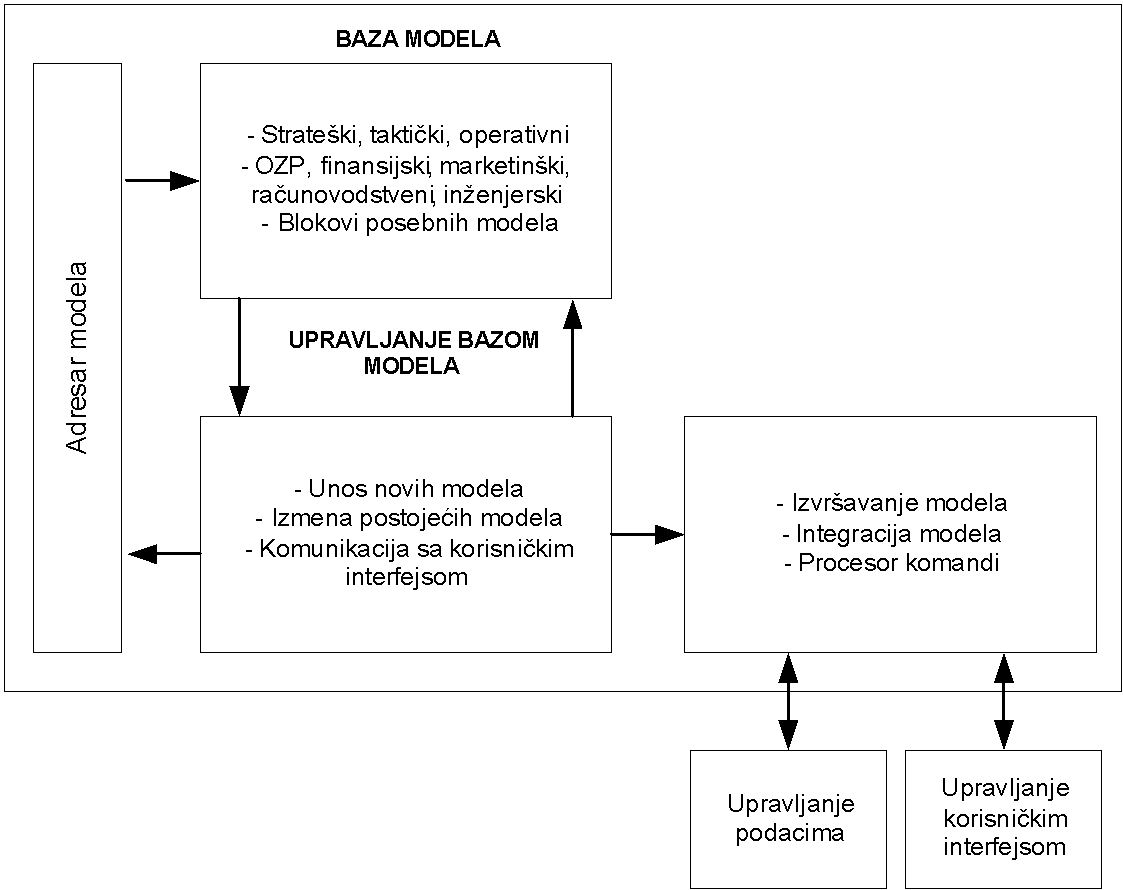
\includegraphics[width=0.85\linewidth]{slike/01/01-23.png}
    \caption{Структура управљања моделима код СПО}
    \label{fig:01-12}
\end{figure}

Објашњавајући БМ и СУБМ, Турбан слично размишља као Спраг и Карлсон. Међутим, интересантна су размишљања о улози адресара модела, која по Турбану треба да буде специфичан каталог свих модела лоцираних у бази модела. Адресар треба да садржи дефиниције модела и његове основне функције, како би одговорио на корисникова питања везана за могућности коришћења и особине модела. Но, и поред тога адресар модела не даје одговор на суштинско питање: „Који модел треба користити, за коју прилику и потребу?“ На исто питање свој одговор не дају ни системи за управљање базом модела (СУБМ), јер да би се такав одговор уопште и могао дати, неопходно је поседовати експертска знања. По Турбану, таква једна чињеница представља и основни разлог за интеграцију експертних система у проблематику управљања моделима СПО.

Последња компонента структуре управљања има три функције:

\begin{itemize}
  \item Извршење модела - контролише извршавање модела.
  \item Интеграција модела - комбинује операције већег броја модела, када је то потребно. Посебно важну улогу у тој интеграцији има коришћење одговарајуће семантике.
  \item Процесор команди се користи за прихватање и интерпретирање моделских инструкција онако како теку од корисничког интерфејса ка СУБМ, извршавању модела и интеграцији модела.
\end{itemize}
Проблем управљања моделима у себи садржи још један суштински проблем. Ако би база модела била „велика“, тј. ако би у себи имала већи број модела, онда би практично корисник морао да их зна све, како би их могао најефикасније и употребити. Но, то је практично немогућ задатак, чак и за експерта из области.

Због тога је било потребно развити специјализовани експертни систем за избор модела из базе модела код СПО. Такав систем је требало да омогући кориснику да кроз неколико корака врши „тријажу“ модела, тј. одбацивање оних модела из базе модела који сигурно нису кандидати да буду коришћени.

Предност оваквог приступа је очигледна. Пре свега није неопходно суштинско познавање већег броја модела, што је по правилу случај када су у питању менаџери тактичког и стратешког нивоа, а они представљају најчешће крајње кориснике оваквих система.

Основни недостатак овог приступа је лежао у чињеници да је било немогуће пројектовати експертни систем којим би се решио проблем општег управљања моделима сваког СПО. За сваку конкретну ситуацију би се морао пројектовати одговарајући ЕС.

\section{Групно одлучивање}
У модерним условима пословања, већину сложених одлука у организацијама доноси специјализована група. Пораст сложености организационог одлучивања утицао је на раст потреба за честим састанцима и групним радом при чему су групе све чешће просторно и/или временски раздвојене (Сукновић и Делибашић, 2011).

Још почетком 2000-их година истраживања су показала да се значајан део сарадње међу запосленима одвија на различитим местима и у различито време. Од тада, овај тренд се драматично убрзао, посебно након глобалне пандемије COVID-19, када је рад на даљину (енг. remote work) и хибридни модел рада постао стандард у многим организацијама. Данас, у већини модерних организација, више од половине колаборације одвија се уз помоћ дигиталних алата, без физичког присуства свих учесника.

Подршка групном раду где чланови тима могу бити на различитим местима и да раде у различито време наглашава важне аспекте комуникације, компјутерских технологија и методологија рада. Ефикасни компјутерски алати за подршку рада групе (енг. groupware) су развијени да би смањили трошкове и омогућили ефикасну размену мишљења, информација, података, знања, докумената и других ресурса који су потребни за рад раздвојених група и/или појединаца. Ови алати могу подржати процес пословног одлучивања:

\begin{itemize}
  \item Индиректно – обезбеђују ефикасну колаборацију уз помоћ технологија као што су имејл (е-пошта), чет, дељење датотека, итд. Међутим ови алати не обезбеђују моделе одлучивања, као ни структуриран процес доношења одлука.
  \item Директно – обезбеђују структуриран и усмерен процес доношења одлука и интегрисане моделе и методе одлучивања чиме се омогућује генерисање решења за конкретан проблем (ГСПО).
\end{itemize}
У наставку ће бити описана оба типа алата за подршку одлучивању. Прво следи објашњење појма колаборације, компјутерских технологија које подржавају колаборацију, као и различити начини класификација ових технологија. Затим се детаљно описују групни системи за подршку одлучивању.

\section{Колаборативни алати за индиректну подршку одлучивању}
Колаборација или сарадња, представља комуникацију и координацију јединица унутар групе ради постизања заједничког циља. Јединице могу бити људи који чине тим, повезане организације, земље, заједнице, рачунари, роботи, итд.

У данашњим условима пословања неопходно је користити технологије (најчешће дигиталне) које омогућавају ефикаснију и ефективнију колаборацију, а самим тим и постизање циљева групе. Неке од технологија су: имејл, веб сајтови, тренутне поруке (енг. Instant messaging - IM), чет, е-групе, вики (енг. wiki) сајтови, форуми, дељени документи, дељене апликације, системи за управљање задацима и пројектима, виртуелне собе за састанке, итд.

У (Сукновић, 2001) предложен је временско-просторни оквир за класификацију алата за подршку рада групе (слика 1.15):

\textbf{Исто време/исто место (нпр. соба за одлучивање)}

Учесници се налазе у исто време на истом месту, као на традиционалним састанцима.

\textbf{Исто време/различито место (нпр. телеконференција)}

Учесници се налазе на различитим местима али комуницирају у исто време.

\textbf{Различито време/исто место (нпр. локална рачунарска мрежа)}

Учесници раде у сменама. Једна смена оставља информације наредној.

\textbf{Различито време/различито место (нпр. удаљено одлучивање)}

Учесници се налазе на различитим локацијама и деле информације асинхроно.

\begin{figure}[h]
    \centering
    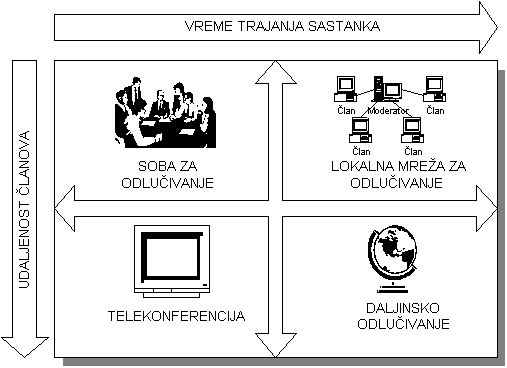
\includegraphics[width=0.85\linewidth]{slike/01/01-27.png}
    \caption{Врсте ГСПО апликација на основу критеријума удаљеност чланова-време трајања састанка}
    \label{fig:01-13}
\end{figure}

Технологије комуникације, зависно од природе проблема који помажу, могу се класификовати на:

\begin{itemize}
  \item синхроне и асинхроне,
  \item трајне (перзистентне) и привремене, и
  \item са кардиналношћу 1-1, 1-М, М-М.
\end{itemize}
Синхрони облици комуникације захтевају од свих учесника да истовремено буду присутни док се комуникација одвија. У ту класу би спадали: тренутне поруке, аудио/видео конференције, четови, итд.

Асинхрони облици омогућују учесницима да у различито време шаљу и примају поруке. У ове облике се могу сврстати: веб сајтови, е-пошта, форуми, итд.

Перзистентни облици комуникације чувају поруке на дуже време лако доступним. Од технологија за пренос трајних порука могу се користити веб и вики стране, дељени документи, итд.; док за привремене поруке могу да се користе форуми, е-групе, чет, имејл, итд.

Додатно, проблеме комуникације можемо поделити на оне који преносе поруке између два члана (1-1); између једног и више чланова (1-М); или поруке које више чланова преноси до више примаоца (М-М).

\section{Групни системи за подршку одлучивању}
Јака експанзија развоја информационих технологија, и уклањање временско-просторних баријера уз помоћ колаборативних алата, омогућили су развој групних система за подршку одлучивању (ГСПО). Прва истраживања у свету на ову тему заслуга су (Zelenny, 1982) са акцентом на употребу разноврсних модела групног одлучивања. Темеље за будућа истраживања поставили су (DeSanctis \& Gallupe, 1987).

\textbf{Групни системи за подршку одлучивању су интерактивни системи базирани на употреби информационе технологије и прецизног алгоритма одлучивања, а изграђени су на идеји индивидуалног (појединачног) СПО. Њихов основни задатак је да олакшају решавање полуструктурираних и неструктурираних проблема заједничким радом групе.}

Према (Theireuf, 1989), „ГСПО има за циљ да побољша групно одлучивање, уклањањем уобичајених комуникационих баријера, пружањем техника за структурирање анализе одлучивања и системско одређивање начина, времена и садржаја дискусије у циљу добијања већег квалитета одлуке“.

Битне карактеристике ГСПО, према (Сукновић, 2001) су:

\begin{itemize}
  \item ГСПО је посебно дизајниран систем, а не само склоп постојећих система.
  \item ГСПО је пројектован са циљем да помаже доносиоцима одлука у њиховом раду.
  \item ГСПО усклађује знања различитих корисника, те уз примену рачунара, омогућује бољу подршку одлучивању.
  \item ГСПО може бити специфичан (дизајниран за један тип проблема) или општи (дизајниран за различите одлуке на нивоу групе).
  \item ГСПО садржи уграђене механизме који обесхрабрују развој негативних понашања у групи.
\end{itemize}
Унапређење процеса групног одлучивања употребом ГСПО, према (Сукновић, 2001) су следеће:

\begin{itemize}
  \item Чланови тима раде паралелно, тако да је могуће добити много идеја,
  \item Захваљујући анонимној идентификацији, чланови тима су неоптерећени моћи и статусом појединих чланова,
  \item Повећана ефикасност групе, због структурираног и контролисаног процеса одлучивања,
  \item Систем даје на располагање члановима тима лепезу метода, модела и техника за решавање проблема,
  \item Отвореност система омогућава константан проток нових информација,
  \item Систем омогућава складиштење података на сваком нивоу процеса одлучивања,
  \item Повећава се продуктивност рада поготово због скраћеног времена трајања састанка, итд.
\end{itemize}

\subsection{Основне компоненте групних система за подршку одлучивању}
Без обзира на различите конфигурације ГСПО, његове основне компоненте су: хардвер, софтвер, људи и процедуре.

Групи, као целини или сваком њеном члану, мора да буде омогућен приступ рачунару ради презентације релевантних података. Минимални хардверски захтеви система су: У/И јединица, процесор, веза између У/И јединица и процесора и заједнички екран или монитор за сваког члана групе.

Системска софтверска компонента ГСПО подразумева систем за управљање базом података и базом модела, као и специјализовану корисничку апликацију која подржава рад групе. Најзначајнија технолошка компонента ГСПО-а је специјално развијен апликативни софтвер, који подржава групу у процесу доношења одлука.

„Људска“ компонента ГСПО подразумева чланове групе и модератора који је одговоран за беспрекорно функционисање ГСПО технологије. Модератор има веома флексибилну улогу. Присутан је на свим групним састанцима и има улогу да управља ГСПО хардвером и софтвером.

Процедуре, као компонента ГСПО, имају задатак да олакшавају ефективно коришћење технологије.

\subsection{Технологија групних система за подршку одлучивању}

\begin{figure}[h]
    \centering
    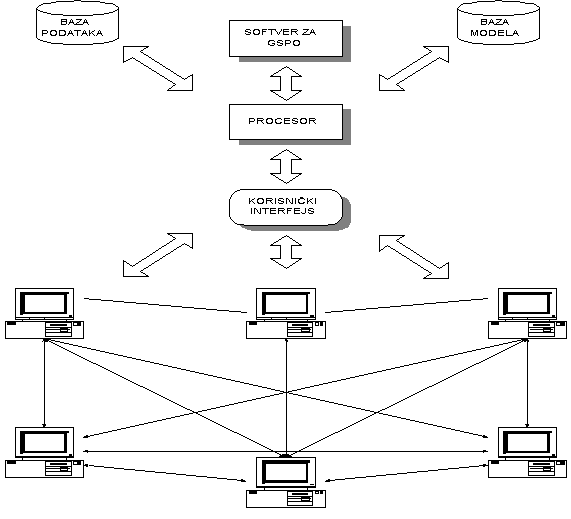
\includegraphics[width=0.85\linewidth]{slike/01/01-18.png}
    \caption{Основна технологија ГСПО}
    \label{fig:01-14}
\end{figure}

Према (Сукновић, 2001) технологија ГСПО подељена је у три нивоа:

\begin{itemize}
  \item 1. ниво - подршка процесу,
  \item 2. ниво - подршка одлучивању,
  \item 3. ниво - правило „реда“, односи се на контролу времена, садржаја дискусије, правила гласања, итд.
\end{itemize}
ГСПО првог нивоа обезбеђују техничке карактеристике за уклањање уобичајених комуникационих баријера, као што су велики екрани за тренутно приказивање идеја, сумирање гласова, анонимно уношење идеја и преференци, размена електронских порука између чланова групе, итд.

ГСПО другог нивоа обезбеђује моделирање одлука и техника групног одлучивања у циљу смањивања несигурности. За разлику од ГСПО првог нивоа који је само комуникациони медиј, ГСПО другог нивоа представља његово знатно проширење.

ГСПО трећег нивоа карактеришу стандардни обрасци за комуникацију у групи. Ови системи укључују и савете експерата у вези са избором и креирањем правила која ће се користити током састанка.

Што је већи ниво ГСПО, технологија мора бити савременија, али је и утицај на природан процес доношења одлука у групи све већи.

\subsection{Структура групних система за подршку одлучивању}
Сложеност процеса групног одлучивања умногоме модификује стандардну процедуру употребе индивидуалних система за подршку одлучивању. Према (Bui, 1987), та модификација варира у шест типова комуникације корисника и СПО.

\begin{figure}[h]
    \centering
    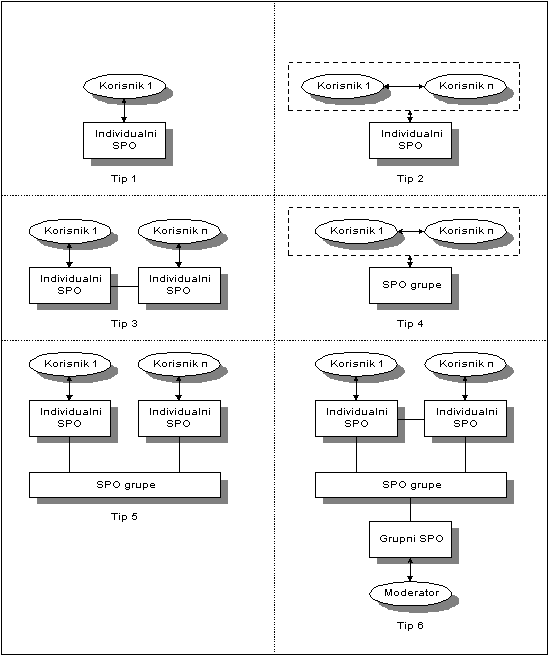
\includegraphics[width=0.85\linewidth]{slike/01/01-19.png}
    \caption{Типови комуникације корисник-СПО}
    \label{fig:01-15}
\end{figure}

Основни елементи који прате сваку развијену апликацију ГСПО су брзина реализације процеса групног одлучивања и тачност добијеног решења. Према (Сукновић, 2001), постоји пет варијанти структура одлучивања. Показало се да је структура звезда најефективнија код решавања структурираних и полуструктурираних проблема. Док структура точак највише одговара за неструктуриране и креативне ситуације одлучивања.

\begin{figure}[h]
    \centering
    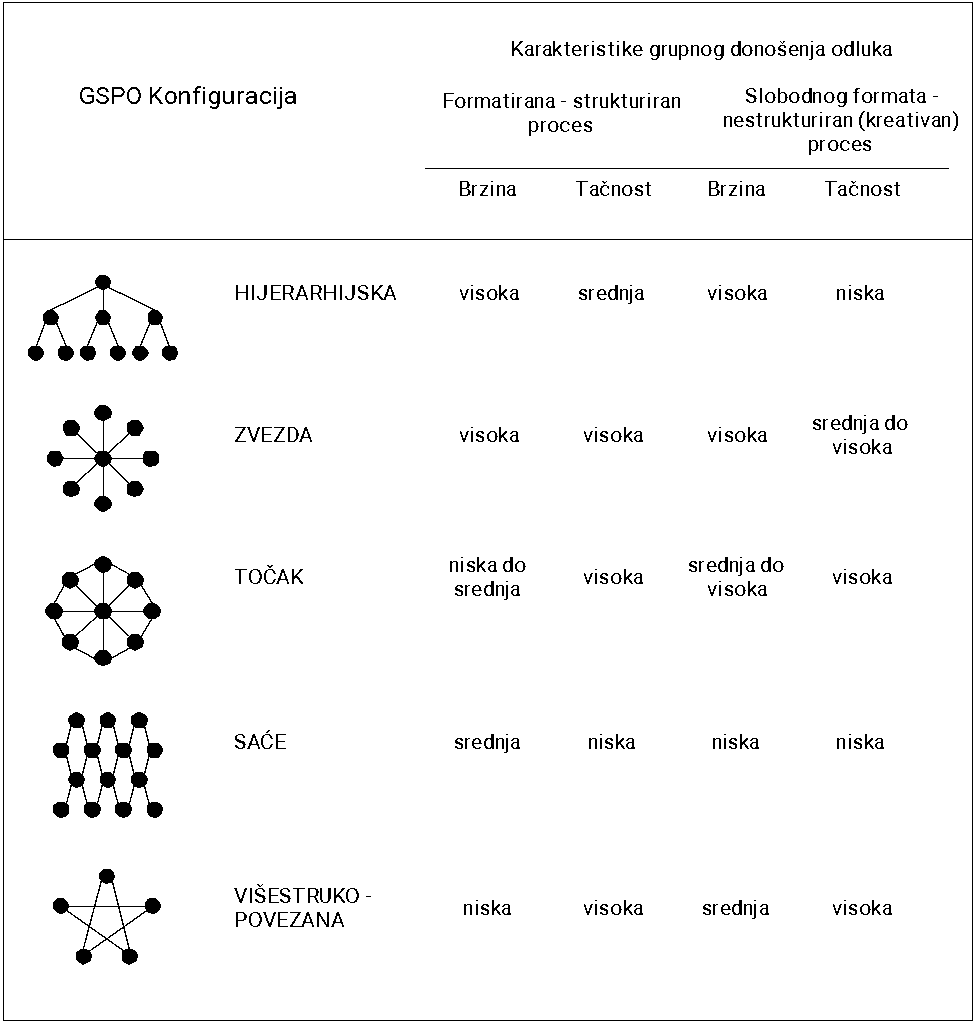
\includegraphics[width=0.85\linewidth]{slike/01/01-32.png}
    \caption{Могуће структуре одлучивања употребом ГСПО}
    \label{fig:01-16}
\end{figure}

\subsection{Пример архитектуре ГСПО и процеса одлучивања уз помоћ ГСПО}
Према (Bui, 1987), имплементација ГСПО може се базирати на моделима вишекритеријумског одлучивања. Тако ГСПО представља мрежу процесно оријентисаних индивидуалних СПО. Сваки учесник групног процеса одлучивања има сопствени СПО чија се база модела заснива методама и моделима вишекритеријумског одлучивања.

\begin{figure}[h]
    \centering
    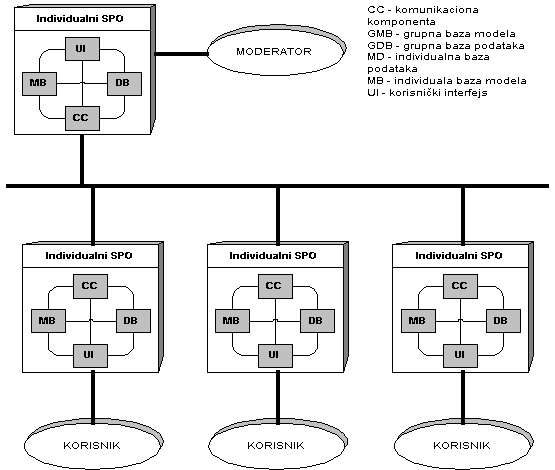
\includegraphics[width=0.85\linewidth]{slike/01/01-03.png}
    \caption{Могућа архитектура ГСПО - Тип 6 (Bui, 1987)}
    \label{fig:01-17}
\end{figure}

\begin{figure}[h]
    \centering
    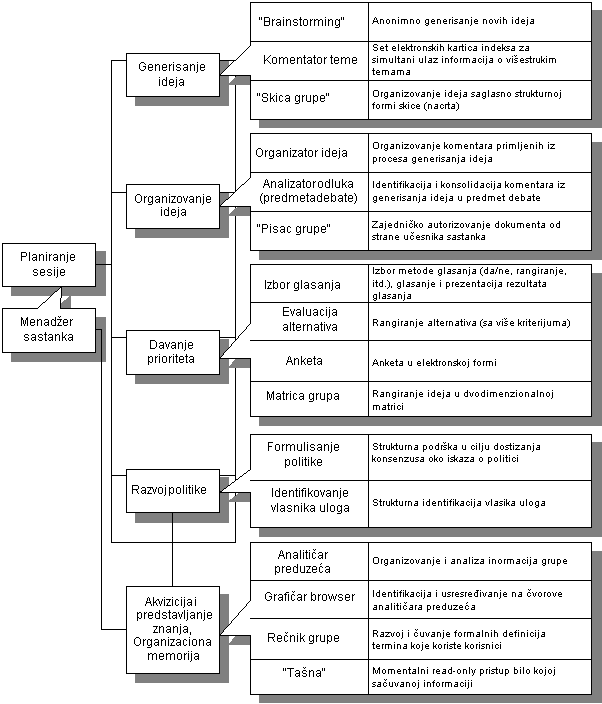
\includegraphics[width=0.85\linewidth]{slike/01/01-11.png}
    \caption{Неопходни модули рада развијене ГСПО апликације}
    \label{fig:01-18}
\end{figure}

\begin{figure}[h]
    \centering
    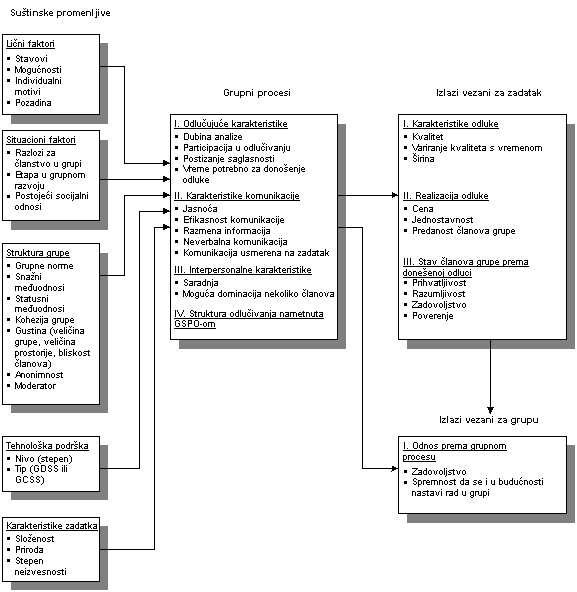
\includegraphics[width=0.85\linewidth]{slike/01/01-15.png}
    \caption{Улазне, процесне и излазне променљиве ГСПО}
    \label{fig:01-19}
\end{figure}

\subsection{Улога и задатак групе у формирању ГСПО}
Задатак са којим се сусреће група мора да буде покретачка снага за дизајнирање ГСПО. Карактеристике задатка одређују потребу за информацијама и начин комуникације у групи која доноси одлуке.

Главни циљеви групе према (Сукновић, 2001) су:

\begin{itemize}
  \item генерисање идеја и алтернатива (креативни задаци захтевају генерисање нових идеја, док плански задаци захтевају генерисање планова оријентисаних на алтернативе);
  \item избор алтернатива (решавање и примена решења подразумева избор најприхватљивије алтернативе);
  \item преговарање о алтернативама (сазнајно-конфликтни задаци подразумевају приближавање супротстављених гледишта).
\end{itemize}
Предности примене ГСПО према (Сукновић, 2001) су:

\begin{itemize}
  \item олакшавају и поједностављују унос и приказ идеја свих чланова групе,
  \item повећавају брзину процене идеја,
  \item обезбеђују техничку подршку за активности креативног мишљења,
  \item поседују могућност избора исправног решења,
  \item повећавају ефективност решења у задацима преговарања.
\end{itemize}
Са растом притиска да се одлуке доносе у групама, јавља се потреба за развојем и изучавањем система за групно доношење одлука, ослоњених на јаку подршку савремених информационо-комуникационих технологија.

У претходним потпоглављима приказани су системи који подржавају индивидуално и групно доношење одлука – СПО, ЕС и ГСПО. Сви ови системи имају заједнички циљ: да доносиоцу одлуке омогуће приступ потребном знању за доношење исправне управљачке пословне одлуке. На самом почетку овог поглавља дефинисана је пословна интелигенција као скуп технологија, организационих правила и знања удружен у генерисању знања за доношење одлуке. Такође, у потпоглављу о експертним системима, детаљно је описано како се знање чува и користи у базама знања. Међутим, до сада није прецизно дефинисано шта је заправо знање у контексту пословне интелигенције, који облици знања постоје и како се знање открива и систематизује. Управо та питања су тема наредних потпоглавља, у којима се формализује појам знања, уводе узори као носиоци знања и представља целокупан модел пословне интелигенције.

\section{Знање у пословној интелигенцији}
Често се корисницима система пословне интелигенције обећава да ће им системи пословне интелигенције (ПИ) пронаћи знање, које ће омогућити корисницима да боље доносе одлуке. Корисници, са друге стране, често нису ни свесни шта је знање, а ни аналитичари који помажу у откривању знања често не знају шта заправо траже.

У наставку се покушава да се донекле боље објасни шта је знање у пословној интелигенцији, како га препознати и презентовати да би било употребљиво и да би било коришћено у пословном процесу. Сврха система ПИ је пословно обавештавање (кроз управљачке извештаје, откривене законитости, управљачке моделе итд.) са циљем пружања ДО знања које могу довести до одлуке за решавање одређеног пословног проблема.

\section{Врсте знања}
Основа за доношење пословних одлука јесте знање. Циљ подршке одлучивању је предлагање акције (одлуке) коју ДО треба да спроведе када се јави проблем у одређеном контексту.

Око дефиниције знања не постоји општа сагласност. Дефиниција коју ћемо користити за објашњавање знања у пословној интелигенцији је по (Tiwana, 2000):

\textbf{Информација са акцијом расположива у правом формату, у право време и на правом месту за одлучивање.}

Знање је увек везано за контекст, а то значи да знање које важи у одређеном контексту, не мора да важи у другом контексту. Знање представља тројку проблема, контекста и решења. Решење представља предлог акције, који се предлаже ДО.

За знање важи да:

1. Поседовање знања је предуслов доношења исправних управљачких пословних одлука;

2. Знање у себи садржи компоненту акције (решења);

3. Знање је везано за контекст;

4. Знање може да се представи тројком: проблем, контекст и решење;

5. Знање представља прихватљиво решење одређеног проблема, које најчешће није оптимално, и

6. Свако знање тражи одређену емпиријску потврду.

У Табели~\ref{tab:01-3} приказане су неке дефиниције знања на које често може да се наиђе у литератури.

\begin{table}[h]
\centering
\begin{adjustbox}{max width=\textwidth}
\begin{tabular}{|l|l|}
\hline
\textbf{Дефиниција} & \textbf{Аутор} \\
\hline
Способност претварања информација и података у ефективну акцију & (Applehans et al., 1999) \\
\hline
Значајне везе које људи праве у својим умовима између информација и њихове примене у акцију у специфичном контексту & (Dixon, 2000) \\
\hline
Флуидни микс уоквиреног искуства, вредности, контекстуалних информација и експертског увида & (Firestone, 2003) \\
\hline
Знање је информација која је прошла процес валидације & (Firestone, 2003) \\
\hline
Идејна конструкција генерисана преко људског ума & (Housel \& Bell, 2001) \\
\hline
Организациони ресурс састављен од суме онога што се зна & (Holsapple et al., 1996) \\
\hline
Систематизоване и структуриране информације специфичне намене & (Johanessen et al., 2001) \\
\hline
Информација чија је валидност успостављена кроз тестове и доказе & (Liebeskind, 1996) \\
\hline
\end{tabular}
\end{adjustbox}
    \caption{Разне дефиниције знања}
    \label{tab:01-3}
\end{table}

Знање може да се подели на процедурално, дескриптивно, семантичко и епизодно према (Awad \& Ghaziri, 2004).

\textbf{Процедурално знање}

Објашњава процедуру решавања одређеног проблема. Карактеристика овог знања је да оно објашњава како се решава одређени проблем. Ово знање одговара на питање „Како?“, али не и на питање „Зашто?“.

\textbf{Дескриптивно знање}

Описује са више детаља одређени проблем са циљем да се боље објасне појмови везани за конкретну проблематику. Овом знању недостаје организација знања у облику проблем, контекст, решење.

\textbf{Семантичко знање}

Знање код кога су уочене везе и зависности које владају између делова проблема, контекста и решења. Представља надоградњу дескриптивног знања.

\textbf{Епизодно знање}

Састављено из низа повезаних искуствених записа, тј. случајева. Епизоде су одређена искуствена знања. Епизодно знање садржи компоненту акције и представља заправо низ епизода између којих постоји одређени редослед. Епизодно знање је најупотребљивије за доношење пословних одлука.

Циљ је да свако знање пређе пут од процедуралног и дескриптивног до епизодног, да би се на крају проблем који захтева епизодно знање, могао решавати на процедуралан начин.

Претходно описана подела знања може да се објасни на примеру рецепта за пудинг.

\textbf{Процедурално знање (рецепт за пудинг):}

Припремите 0,5 л млека. Одмерите 1 дл хладног млека, додајте садржај кесице и мешајте док маса не постане глатка. Преосталу количину млека засладите са три кашике шећера и загрејте до кључања. Склоните са ватре, умешајте припремљену масу и кувајте два минута уз непрестано мешање. Врелу масу сипајте у влажне посуде и оставите да се пудинг стегне и охлади.

\textbf{Дескриптивно знање:}

Маса је глатка када је смеса за пудинг разложена у маси млека, тј. када је растопљена и не постоје грануле. Врела маса се сипа у влажне посуде да се пудинг не би залепио за ивице посуде.

\textbf{Семантичко знање:}

Постоји веза између ефективности мешања смесе са температуром млека. Маса за пудинг се боље размућује у хладном млеку. Постоји веза између лепљења смесе пудинга за зид посуде и влажности посуде.

\textbf{Епизодно знање (четири епизоде):}

1. Раздвој у делове -> 2. Корак по корак -> 3. Направити прелаз -> 4. Расподелити равномерно

\begin{figure}[h]
    \centering
    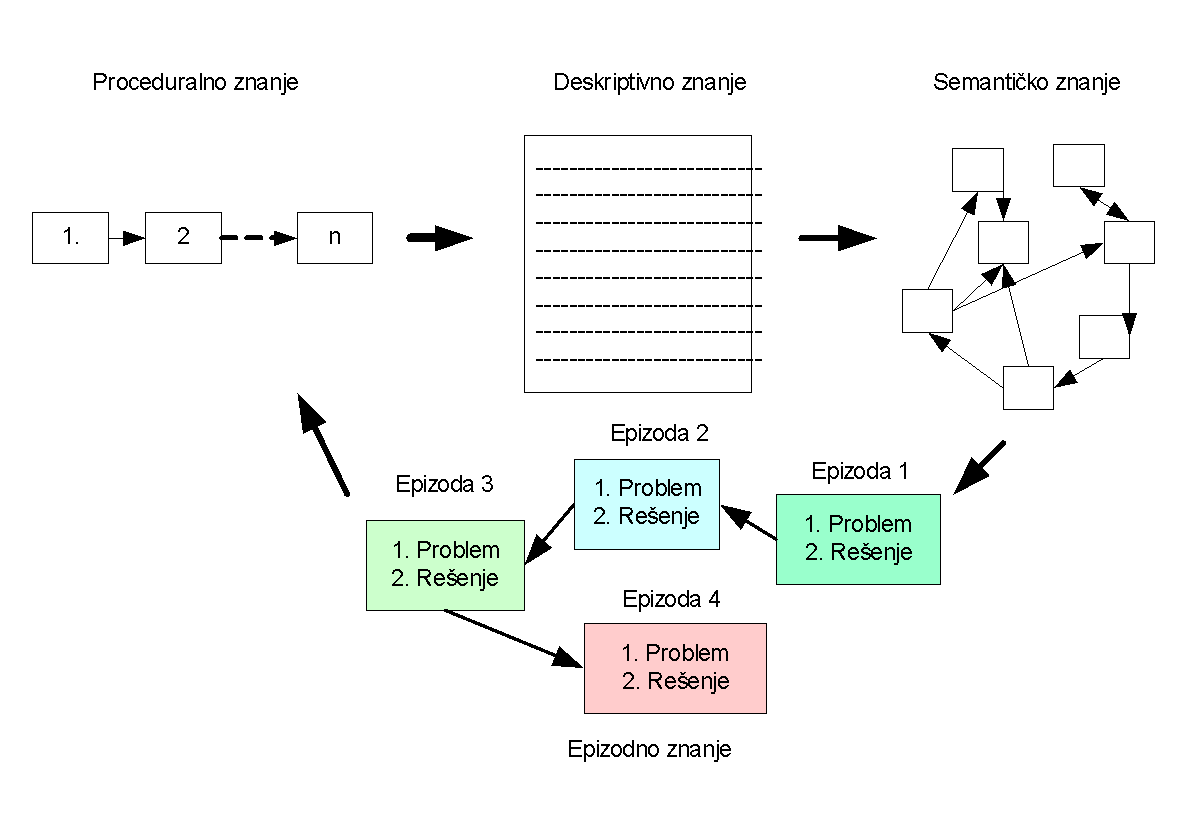
\includegraphics[width=0.85\linewidth]{slike/01/01-04.png}
    \caption{Од процедуралног до епизодног знања и назад}
    \label{fig:01-20}
\end{figure}

Једна од најпознатијих подела знања у свету менаџмента знања је подела на експлицитно и прећутно (подразумевано) знање.

\textbf{Експлицитно знање}

Знање садржано у књигама, документима, извештајима, табелама и сл. Може једноставно да се формализује, представи и сачува у електронској форми.

\textbf{Прећутно знање}

Онај део знања појединаца који се теже формализује. То је знање које је прошло искуствену проверу. Најзанимљивији део прећутног знања је експертско знање које има велику вредност.

Савремени развој вештачке интелигенције, посебно великих језичких модела, отвара нове могућности за формализацију и коришћење прећутног знања. Ови модели су обучени на огромним количинама текста и могу да асистирају у процесу екстернализације знања, генерисању извештаја и подршци одлучивању на начине који раније нису били могући.

\begin{figure}[h]
    \centering
    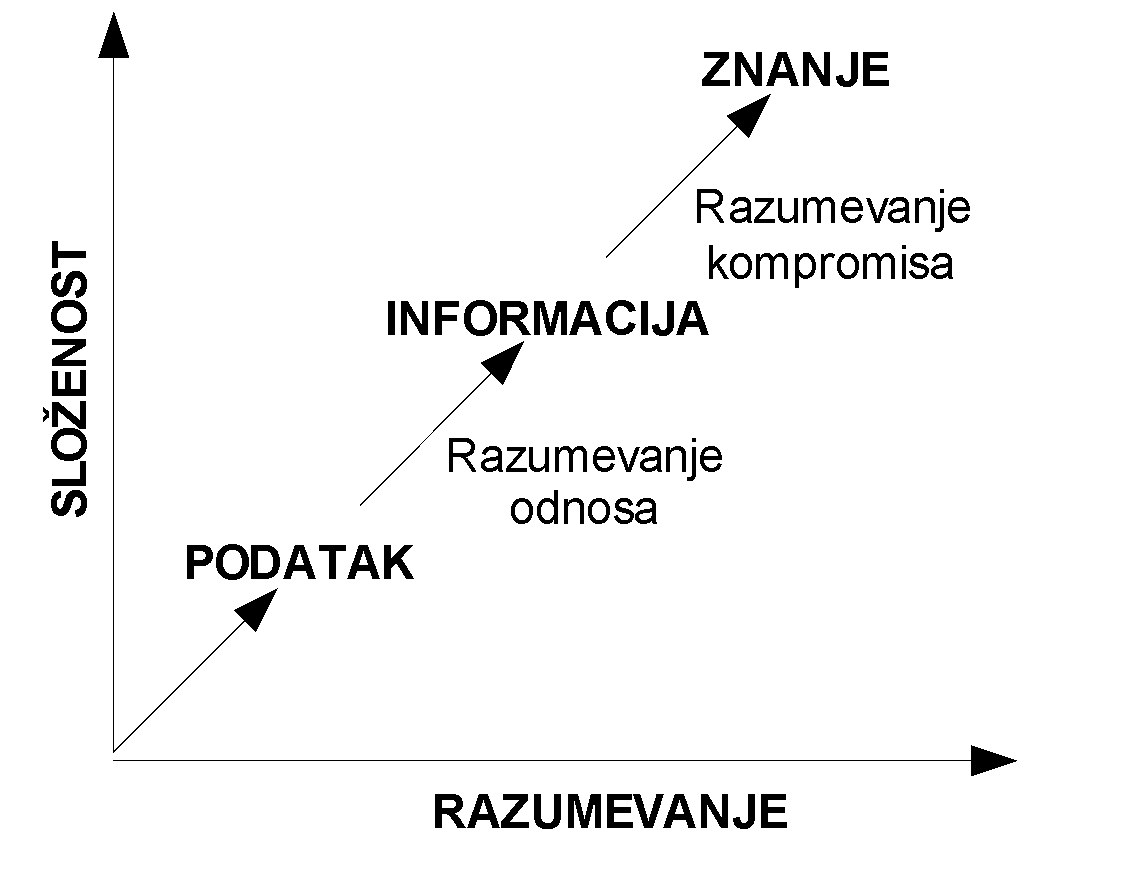
\includegraphics[width=0.85\linewidth]{slike/01/01-24.png}
    \caption{Веза између контекста и разумевања}
    \label{fig:01-21}
\end{figure}

Податак је основни градивни елемент информације и знања. Информација је структура (организован податак). Знање има сложенију структуру од информације, јер садржи и компоненту решења одређеног проблема.

\textbf{Знање садржи компоненту акције. То омогућава подршку одлучивању. Знање је, због тога, основа подршке пословном одлучивању.}

Један облик представљања знања јесте узор. Узор је носилац знања, али је и градивни елемент знања.

\begin{figure}[h]
    \centering
    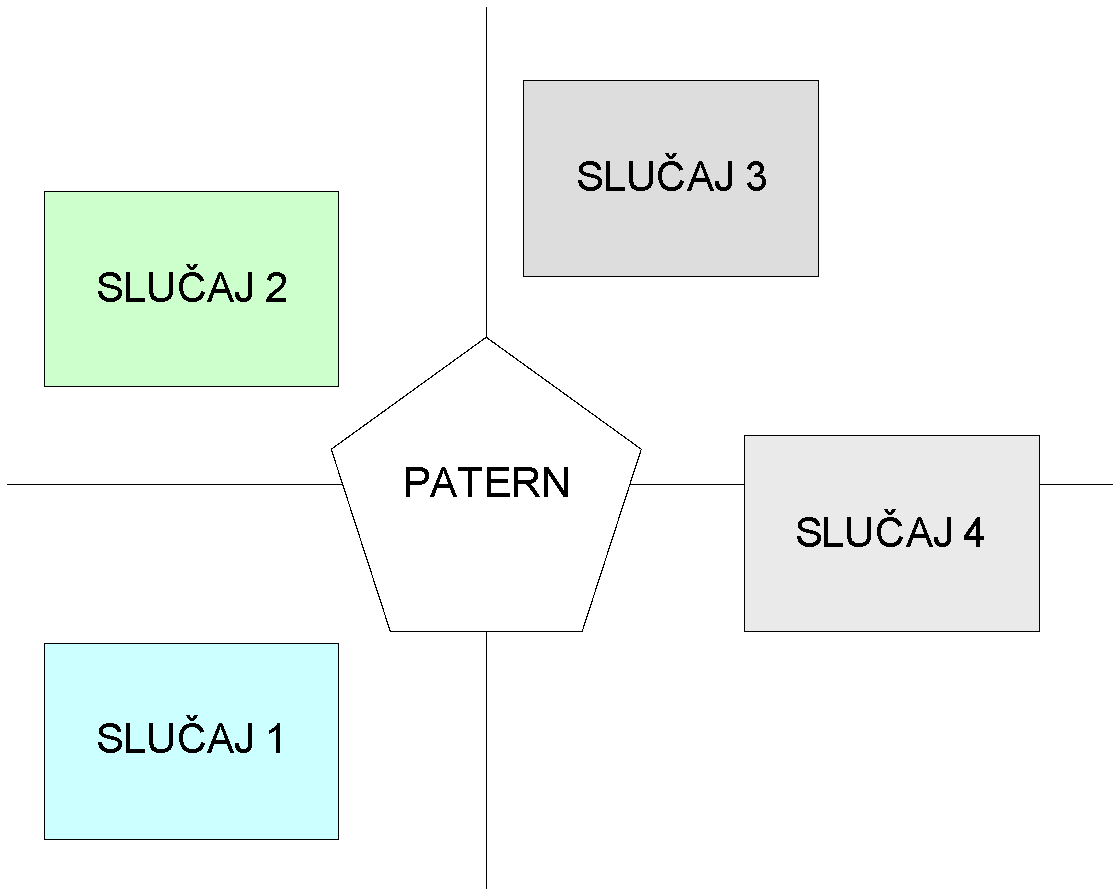
\includegraphics[width=0.85\linewidth]{slike/01/01-21.png}
    \caption{Случајеви теже узорима}
    \label{fig:01-22}
\end{figure}

\section{Узори}
По (Делибашић, 2007), узори представљају искуствено доказана решења за проблеме у одређеном контексту. Могу да се представе тројком \{проблем, контекст, решење\}. За разлику од случајева и других облика знања који имају сличну форму, узори су прошли искуствену валидацију.

Знање експерта може да се моделира преко узора. Сваки експерт је током свог процеса учења савладао одређени број узора који га чине експертом у тој области.

Данас се узори проучавају највише у софтверском инжењерству. Примећено је да се одређена искуствена проверена решења понављају у различитим софтверима, те да их је могуће уочити и делити са осталим софтверским инжењерима.

Идеја творца узор покрета Кристофера Александера (Alexander, 1964, 2002) је да нађе фундаменталне законитости по којима природа и људи стварају.

\begin{figure}[h]
    \centering
    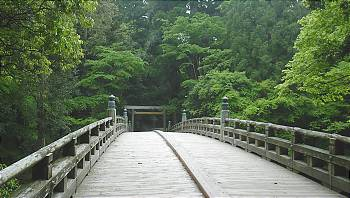
\includegraphics[width=0.85\linewidth]{slike/01/01-05.png}
    \caption{Мост храма Исе Јингу у Јапану}
    \label{fig:01-23}
\end{figure}

\begin{figure}[h]
    \centering
    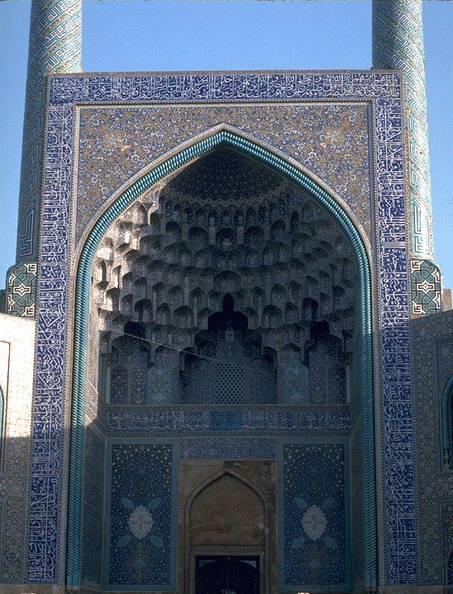
\includegraphics[width=0.85\linewidth]{slike/01/01-07.png}
    \caption{Џамија Масјид-и-Схах у Ирану}
    \label{fig:01-24}
\end{figure}

Ако се у области као што је архитектура могу утврдити законитости по којима треба градити и решавати проблеме, тада се и у свим осталим областима може урадити исто.

Два су појма кључна за схватање Александерове теорије. То су целина и узор. Александер изводи следеће закључке:

1. Узори су искуствена решења.

2. Узори се надопуњују: постојање и функционисање једног узора утиче на други узор.

3. Узори су састављени од узора и

4. Целина добија своју животност с обзиром на густину и интензитет узора који постоје унутар ње.

Скуп узора који чине једно решење једног проблема назива се узор језик. У (Winn \& Calder, 2002) су предложене неке особине које треба да има узор:

1. Треба да буде алат направљен за решавање одређеног проблема.

2. Треба да повезује различите нивое апстракције решења.

3. Садржи и функционалне и нефункционалне особине.

4. Препознатљивост у решењу.

5. Решава битне одлуке код пројектовања решења.

6. Представља део узор језика.

7. Искуствено је проверен.

8. Везан је за одређени домен.

9. Представља значајну идеју.

\section{Узори одлучивања}
Код пројектовања универзитетског насеља Ејшин код Токија пројектанти су пошли од својих корисника и анализирајући навике и потребе корисника, архитекте су смислиле начин како да изграде насеље које у саме грађевине уноси функционалности које подржавају живот класичног јапанског студента.

\begin{figure}[h]
    \centering
    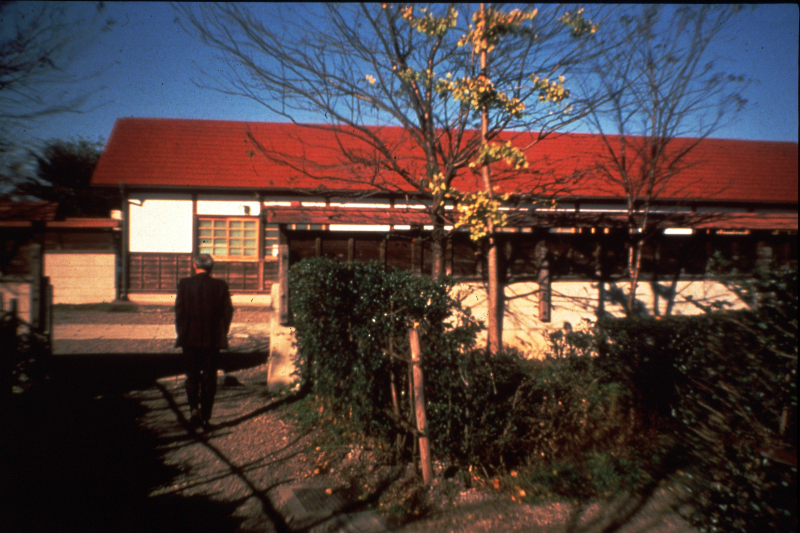
\includegraphics[width=0.85\linewidth]{slike/01/01-17.png}
    \caption{Слике универзитетског насеља (Ејшин кампус)}
    \label{fig:01-25}
\end{figure}

Ако се направи аналогија са одлучивањем, може да се каже да је већина алгоритама за подршку одлучивању направљена од стране научника који не познају већину захтева корисника.

Пример једног узора у Коплиеновој форми:

\textbf{Ко испадне из строја, остаје ван строја.}

1. Контекст: Узор се користи у редно везаним системима.

2. Проблем: Како да систем остане ефикасан када један члан кочи цео систем?

3. Силе: Снага редно везаног система је једнака снази најслабијег објекта.

4. Решење: Избацити објекат из система, вратити га на крај реда.

5. Резултујући контекст: Избацивањем објекта који успорава систем, систем функционише ефикасније.

\subsection{Четири узора одлучивања и процес откривања знања}
Четири узора која се јављају у процесу одлучивања су:

1. Divide et Impera (Подели и владај), Анализа,

2. Додели заједничку вредност,

3. Сви као један (Агрегација) и

4. Анализа.

\textbf{Divide et Impera (подели и владај) - Анализа}

Један од најраспрострањенијих узора у природи. Сваки проблем који се јавља у животу, обично је такав да треба да се растави на мање делове да би био савладив. Код подршке одлучивања и пословне интелигенције, овај узор има велику улогу у дефинисању структуре проблема која је управљива.

\begin{figure}[h]
    \centering
    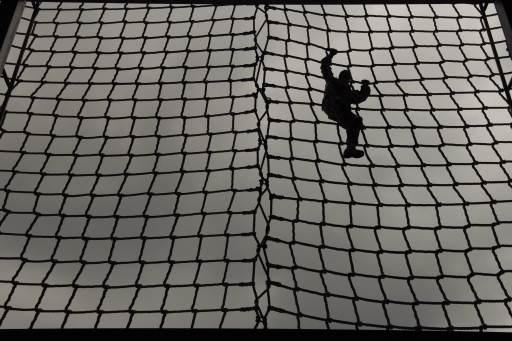
\includegraphics[width=0.85\linewidth]{slike/01/01-06.jpg}
    \caption{Зид који треба савладати}
    \label{fig:01-26}
\end{figure}

\textbf{Додели заједничку вредност - Нормализација}

Овим узором, који се често зове и нормализација, свим подацима се додељују заједничка обележја. Сви подаци који чине базу података за одлучивање добијају заједничку меру преко којих сви подаци могу да се изразе. Ово је потребно ради остваривања могућности да се упоређују подаци.

\begin{figure}[h]
    \centering
    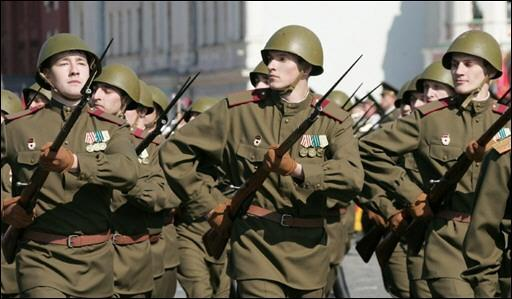
\includegraphics[width=0.85\linewidth]{slike/01/01-10.jpg}
    \caption{Униформисани војници}
    \label{fig:01-27}
\end{figure}

\textbf{Сви као један (Агрегација) - Синтеза}

Узор који представља функцију која из података извлачи агрегације, тј. решење на основу којих може да се доноси одлука. Ово је синтетичка фаза добијања знања, док је „Дивиде ет импера“ аналитичка фаза, а „Додели заједничку вредност“ повезује аналитичку и синтетичку фазу процеса откривања знања.

\begin{figure}[h]
    \centering
    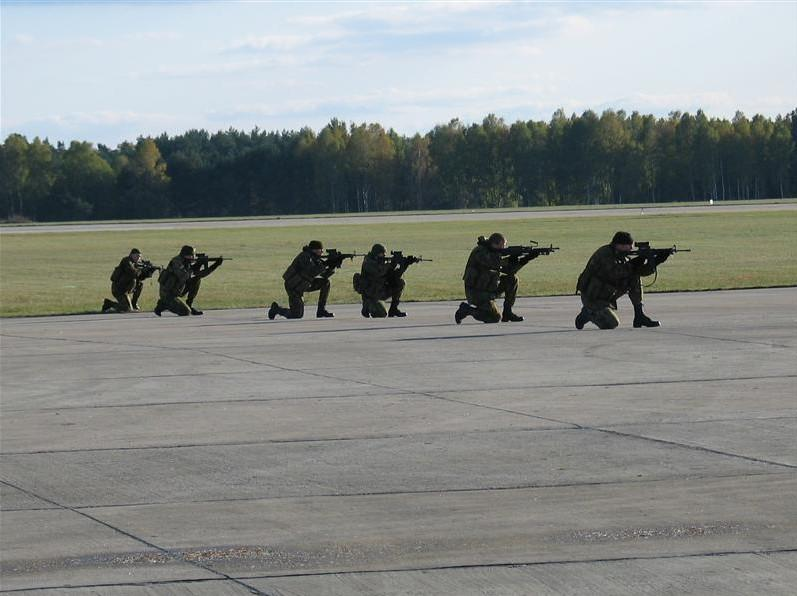
\includegraphics[width=0.85\linewidth]{slike/01/01-08.jpg}
    \caption{Војници у положају за гађање}
    \label{fig:01-28}
\end{figure}

\textbf{Евалуација}

Последњи, али можда и најважнији узор одлучивања. Представља узор који унапређује систем одлучивања. Један је од кључних узора у одлучивању јер показује колико је откривено решење добро или не.

\begin{figure}[h]
    \centering
    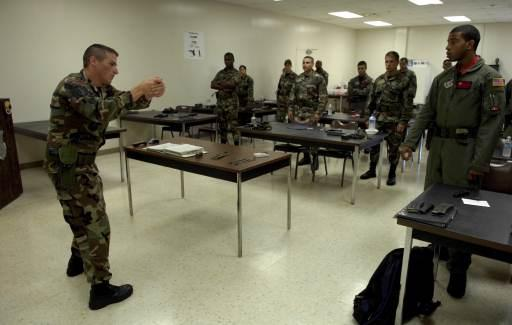
\includegraphics[width=0.85\linewidth]{slike/01/01-14.jpg}
    \caption{Евалуација и припрема за нове задатке}
    \label{fig:01-29}
\end{figure}

\begin{figure}[h]
    \centering
    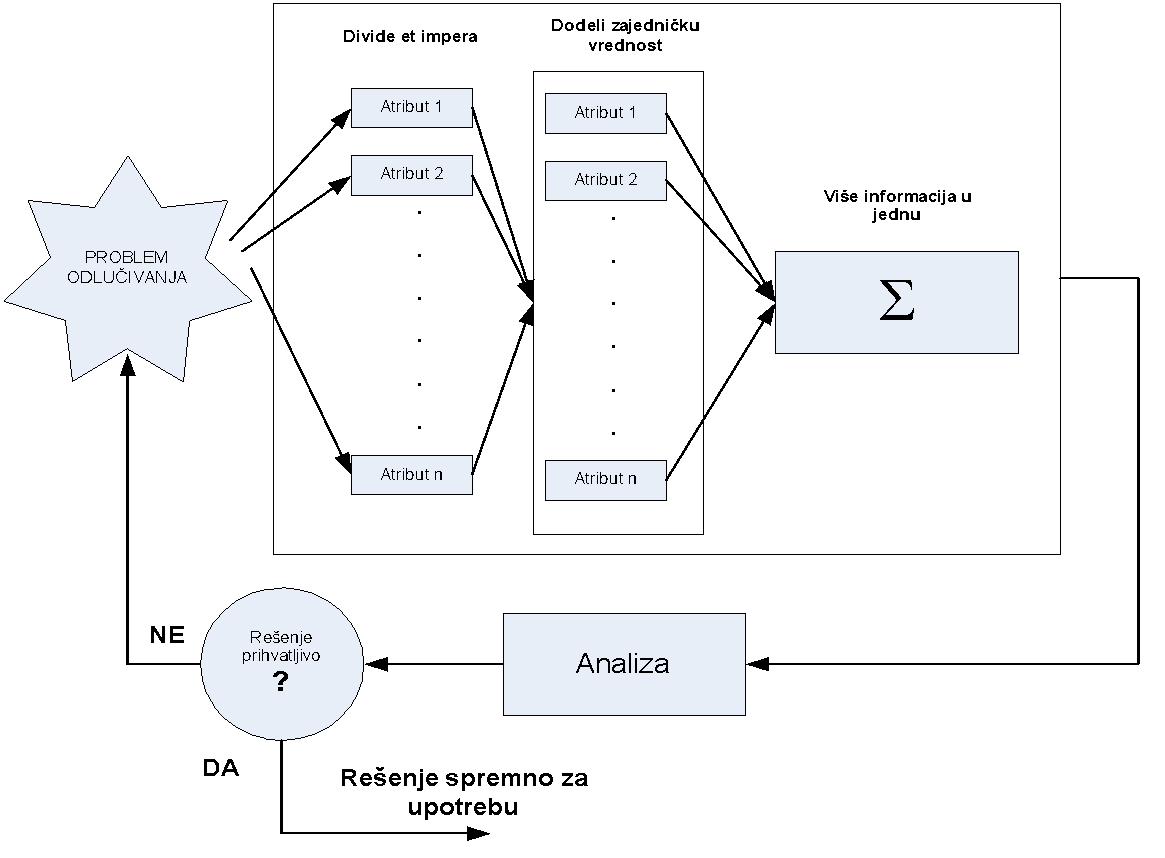
\includegraphics[width=0.85\linewidth]{slike/01/01-01.png}
    \caption{Процес одлучивања преко узора}
    \label{fig:01-30}
\end{figure}

Када постоји проблем, прво се покреће узор „Divide et Impera“. Потом се ради „Додели заједничку вредност“ и „Сви као један“. На крају се узором „Евалуација“ проверава колико је добијено решење добро. Уколико је решење (откривено знање) прихватљиво, процес се зауставља, а уколико не улази се у нову итерацију.

\section{Закључак: Модел пословне интелигенције}
У овом поглављу су представљени системи за подршку одлучивању (СПО и ЕС), системи за подршку групном одлучивању (ГСПО), као и појам знања у пословној интелигенцији. Сви ови концепти конвергирају у моделу пословне интелигенције који следи.

Са циљем да се ДО омогући да доноси исправне управљачке пословне одлуке, могу да се искористе све дисциплине описане у овој књизи.

\begin{figure}[h]
    \centering
    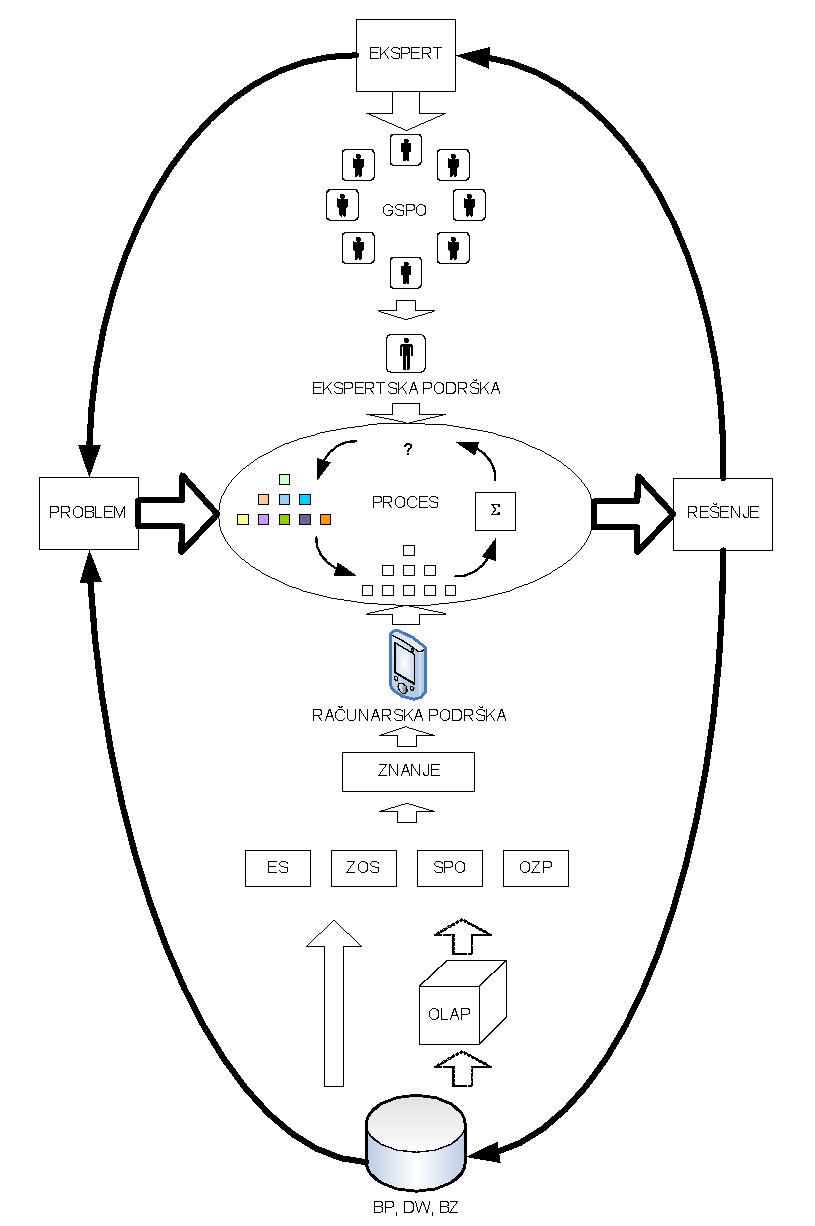
\includegraphics[width=0.85\linewidth]{slike/01/01-02.png}
    \caption{Модел пословне интелигенције}
    \label{fig:01-31}
\end{figure}

Основни циљ ДО је да одређени проблем који се јавља у пословном процесу организације реши у што краћем времену на што бољи начин. То може да уради уколико поседује знање за доношење одлуке.

Централни део слике представља процес откривања знања који је описан преко четири фундаментална узора одлучивања и то „Divide et Impera“, „Додели заједничку вредност“, „Сви као један“ и „Евалуација“.

Модел ПИ пружа ДО подршку у процесу доласка до знања користећи експертску и рачунарску помоћ. Са експертске стране, ДО стоји на располагању или подршка групе или експертска подршка. Сваки пут када група или експерт реше одређени проблем они тиме знање које поседују унапређују.

Са друге стране, рачунарска подршка се заснива на подацима који се прикупљају у базама и складиштима која садрже најзанимљивије податке за анализу и базама знања (БЗ) које чувају ускладиштено знање експерата у одређеној области.

Над складиштем података је могуће изградити ОЛАП коцку. Над ОЛАП коцком је могуће спроводити ОЗП, изградити систем ЗОС. Над базом података и складиштем података је могуће развити систем ЗОС или спроводити ОЗП. Над базом знања је могуће развити експертни систем. СПО је могуће развити над неким моделима које је открио ЗОС или неким другим искуствено провереним моделима које је могуће користити у организацији.

Пословна интелигенција би требало да буде интегрални део сваког информационог система организације. Из тог разлога би све одлуке које се спроводе требало чувати у одговарајућим базама. Ово би омогућило да се знање ефикасно користи и да организација користи пун потенцијал својих кадрова и својих података.

У данашње време, овај модел се проширује новим компонентама. Поред класичних база података и складишта података, организације користе и језера података (Data Lake) за чување неструктурираних података. Алгоритми машинског учења и дубоко учење (Deep Learning) допуњују или замењују класичне ОЗП алгоритме. Системи вештачке интелигенције, укључујући велике језичке моделе, омогућавају конверзацијски приступ подацима где корисник може постављати питања на природном језику и добијати одговоре засноване на анализи података организације. Самоуслужни БИ алати демократизују приступ аналитици, чинећи је доступном ширем кругу запослених у организацији.

Пословна интелигенција је област која се константно развија. Кључни савремени трендови у ПИ укључују:

1. Самоуслужна пословна интелигенција (Self-Service BI): Алати попут Power BI, Tableau и Looker омогућавају крајњим корисницима да сами креирају извештаје и визуализације без помоћи ИТ одељења.

2. Аналитика у облаку (Cloud Analytics): Све више организација мигрира своје БИ системе у облак (AWS, Azure, Google Cloud), чиме се смањују трошкови инфраструктуре и повећава скалабилност.

3. Вештачка интелигенција и машинско учење: Алгоритми машинског учења, укључујући дубоко учење (Deep Learning) и велике језичке моделе (Large Language Models - LLM), аутоматизују откривање законитости у подацима и пружају предиктивну аналитику.

4. Аналитика у реалном времену: Системи за обраду токова података (енг. Stream Processing) омогућавају доношење одлука на основу података који пристижу у реалном времену.

5. Демократизација података: Тренд да сви запослени у организацији имају приступ релевантним подацима и алатима за њихову анализу, а не само специјализовани аналитичари.

\section{Литература}
[1] Делибашић Б (2007) Формализација процеса пословног одлучивања преко патерна, докторска дисертација, ФОН, Београд.

[2] Делибашић Б, Сукновић М, Јовановић М (2009) Алгоритми машинског учења за откривање законитости у подацима, ФОН, Београд.

[3] Сукновић М, Делибашић Б (2010) Пословна интелигенција и системи за подршку одлучивању, Факултет организационих наука, ISBN 978-86-7680-206-7.

[4] Сукновић М, Делибашић Б, Јовановић М, Вукићевић М, Радовановић С (2021) Одлучивање, ФОН, ISBN 978-86-7680-370-5.

[5] Сукновић М (2001) Развој методологије подршке групном одлучивању, докторска дисертација, ФОН, Београд.

[6] Alexander C (1964) Notes on the Synthesis of Form, Harvard University Press.

[7] Alexander C (2002) The Nature of Order Book 1: The Phenomenon of Life, The Center for Environmental Structure, Berkeley California.

[8] Awad E, Ghaziri H (2004) Knowledge Management, Prentice Hall.

[9] Azvine B, Cui Z, Nauck DD, Majeed B (2006) Real time business intelligence for the adaptive enterprise, International Conference on Enterprise Computing.

[10] Bennett J (1983) Building decision support systems, Addison-Wesley, Massachusetts.

[11] Bui TX (1987) Cooperative Co-oP group decision support systems for multiple criteria group decision making, Springer-Verlag, Berlin Heidelberg.

[12] DeSanctis G, Gallupe B (1987) A Foundation For The Study of Group Decision Support Systems, Management Science Vol. 33 No. 5.

[13] Dixon N (2000) Common Knowledge, Harvard Business School Press.

[14] Firestone J (2003) Enterprise Information Portals and Knowledge Management, Butterworth-Heinemann.

[15] Holsapple C, Whinston W, Andrew B (1996) Decision Support Systems - A Knowledge-Based Approach, West Publishing Company.

[16] Housel T, Bell AA (2001) Measuring and Managing Knowledge, McGraw-Hill.

[17] Johannessen J, Olaisen J, Olsen B (2001) Mismanagement of Tacit Knowledge, International Journal of Information Management, Vol. 21, No. 1.

[18] Lawton G (2006) Making business intelligence more useful.

[19] Leigh WE, Doherty ME (1986) Decision Support and Expert Systems, South-Western Publishing Company, Cincinnati, Ohio.

[20] Liebeskind J (1996) Knowledge, Strategy and the Theory of the Firm, Strategic Management Journal.

[21] Meader CL, Guyote MJ, Keen PGW (1984) Setting Priorities for DSS Development, MIS Quarterly 8, str. 117-131.

[22] Simon HA (1945) Administrative Behavior, Free Press, New York.

[23] Sprague RH, Carlson ED (1982) Building Effective Decision Support Systems, Prentice Hall, Englewood Cliffs.

[24] Roland RJ (1982) A model of organizational variables for DSS, Data Base 12, str. 63-72.

[25] Theireuf RJ (1989) Group decision support systems for effective decision making, Quorum Book.

[26] Tiwana A (2000) The Knowledge Management Toolkit, Prentice Hall.

[27] Turban E, Carlson JG (1989) Interactive Visual Decision-Making, U knjizi: Decision Support Systems, Prentice Hall, New Jersey.

[28] Turban E, Aronson JE, Liang TP, Sharda R (2006) Decision Support and Business Intelligence Systems, Prentice Hall.

[29] Winn T, Calder P (2002) Is this a pattern?, IEEE Software.

[30] Zelenny M (1982) Multiple Criteria Decision Making, McGraw-Hill, New York.

% Аутоматски генерисано из Visualization and Data Warehousing.sr.docx

\chapter{Системи извештавања и Складишта података}
\label{ch:skladista}
Савремене организације свакодневно генеришу велике количине трансакционих, оперативних и спољашњих података. Сама количина података, међутим, не доноси аутоматски и боље одлуке: руководиоци, аналитичари и оперативно особље суочавају се са проблемом како из тих података брзо извући информацију која је релевантна за конкретну одлуку коју треба донети. Управо овај раскорак — између расположивих података и употребљиве информације — представља основни мотив за интегрисани приступ извештавању који комбинује визуелизације, контролне табле и складишта података (Few, 2012; Kimball \& Ross, 2013).

Визуелизације служе да се сложени односи међу подацима преведу у облик који људски визуелни систем може брзо да обради. Тренд, одступање, груписање или изузетак који се у табели од хиљаду редова не би лако уочили, на одговарајуће изабраном графикону постају видљиви на први поглед. Контролне табле тај принцип подижу на ниво пословног процеса: уместо једног графикона, оне обједињују скуп међусобно повезаних показатеља на једном екрану и омогућавају доносиоцу одлуке да у реалном времену прати стање посла и реагује на одступања. Складишта података чине овакво извештавање одрживим на нивоу целе организације — обједињавањем података из различитих оперативних система у конзистентан, аналитички организован модел, она обезбеђују да сви извештаји говоре о истим бројевима и да упити над великим обимом историјских података буду брзи.

Размотримо једноставан пример. Менаџер продаје велике малопродајне мреже жели да одговори на питање: „Који производи у којим регионима су у последњем кварталу подбацили план продаје и какав је тренд у претходних шест месеци?” Без интегрисане инфраструктуре, тај одговор подразумева ручно прикупљање извештаја из неколико оперативних система, спајање у табеларном калкулатору и израду графикона за сваки регион појединачно — поступак који траје данима и при сваком новом питању се понавља. Са складиштем података које обједињује продају, планове и димензије производа и региона, исти упит се извршава за неколико секунди; контролна табла приказује одступање од плана по регионима бојом и величином, а низ малих графикона уз сваки регион показује кретање у шест месеци. Менаџер у једном погледу види где је проблем и може одмах да пређе на питање зашто, уместо да троши време на питање колико.

Ово поглавље прати ову логику. У одељку 2.1 разматра се корисничка страна — визуелизације, њихово кодирање, интерактивни прикази и контролне табле — односно средства којима подаци постају информација. У одељку 2.2 представљена је инфраструктурна страна — складишта података, OLAP коцке и методологије изградње — без које ефикасно извештавање на нивоу предузећа није могуће. Циљ поглавља је да покаже да су ове две перспективе нераздвојиве: добра визуелизација над лошим подацима обмањује, а добро складиште без употребљивих визуелизација остаје неискоришћен ресурс.

\section{Извештавање и визуелизације}
Извештавање је основна форма употребе пословних података: његов задатак је да доносиоцу одлуке у тренутку када му је потребна пренесе тачну, сажету и разумљиву слику стања посла. У овом одељку извештавање се посматра из угла корисника — од основа визуелне перцепције и типова података, преко избора графикона и визуелног кодирања, до сложенијих облика приказа какви су вишедимензионални прикази, приповедање подацима, интерактивне визуелизације, пивот табеле и контролне табле. Циљ је да се изложе принципи који доброј визуелизацији дају информациону вредност и да се представе технике и алати помоћу којих се од сирових података долази до извештаја који заиста подржава одлучивање (Few, 2012; Munzner, 2014).

\subsection{Основе визуелизације}
Визуелизација података је начин да податке видимо, лакше разумемо и брже протумачимо. Уместо да аналитичар или доносилац одлуке пролази кроз дуге табеле и низове бројева, графикон, карта или контролна табла могу му одмах показати тренд, разлику, одступање или проблем. Зато визуелизација није само „улепшан” приказ резултата, већ практичан део анализе који помаже да се из података дође до смисленог закључка (Few, 2012; Munzner, 2014).

Разлог је једноставан: људи брже уочавају образац на слици него у табели. Када су подаци приказани положајем, дужином, бојом или обликом, лакше примећујемо раст, пад, груписање и изузетке него када исте информације читамо ред по ред. Због тога добра визуелизација смањује напор потребан за разумевање података и оставља више простора за само расуђивање (Ware, 2013; Card, Mackinlay, \& Shneiderman, 1999).

Зато се може рећи да визуелизација има четири једноставне улоге: 

\begin{itemize}
  \item \textbf{\textit{помаже бржем уочавању образаца, }}
  \item смањује оптерећење при читању података, 
  \item \textbf{\textit{подстиче нова аналитичка питања и }}
  \item служи као радни простор за размишљање, а не само као приказ коначног резултата.
\end{itemize}
Визуализације омогућавају аналитичару да постепено поставља све боља питања. Док посматра графикон, он може да примети нешто неочекивано, да издвоји сумњив (или екстреман) случај, да упореди групе или да се врати на податке са новим питањем. У том смислу, визуелизација није само завршни корак анализе, већ и средство помоћу којег анализа напредује.

\textbf{\textit{Пример: }}аналитичар продаје посматра линијски графикон укупног месечног прихода и примећује нагли пад у марту. То га наводи на следеће питање — да ли је пад равномеран по регионима или је концентрисан на једном тржишту. Прелазак на групирани стубичасти графикон по регионима открива да је пад готово у целости везан за један регион, док остали бележе благи раст. Ново питање које се природно намеће јесте да ли је реч о свим производним категоријама или само о некима — топлотна мапа категорија по недељама у том региону показује да је пад скоро у потпуности последица једне категорије у две конкретне недеље. Аналитичар тада зна где даље да тражи узрок (нпр. застој у снабдевању или промена цене код конкурента), иако први график није ни наговестио тако специфичан узрок. Свака следећа визуелизација била је одговор на питање које претходна није могла да постави, што илуструје како визуелизација води анализу, а не само закључује.

Експоненцијални раст података у погледу обима, брзине и разноврсности — често описан као „велики подаци” (енг. \textbf{\textit{big data}}) — значајно је повећао сложеност аналитичких задатака. Савремене организације прикупљају податке из трансакционих система, сензора, платформи друштвених мрежа и дигиталних услуга, што резултира скуповима података који су превелики и превише сложени да би се разумели само традиционалним табеларним прегледом (Chen, Chiang, \& Storey, 2012).

\begin{figure}[h]
    \centering
    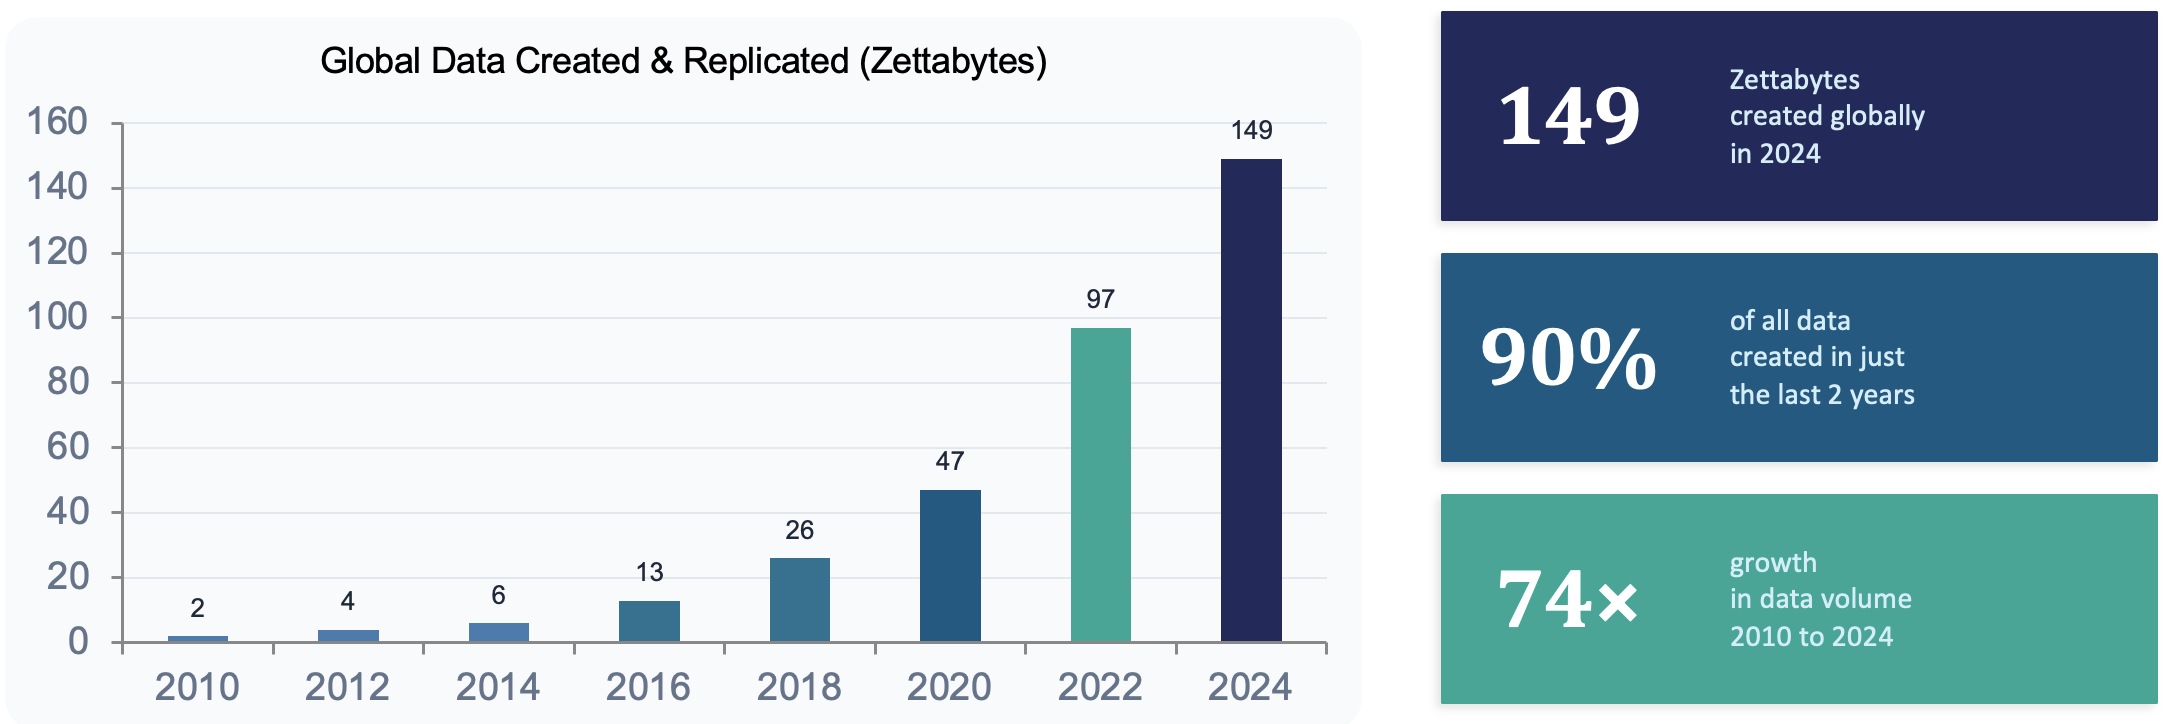
\includegraphics[width=0.85\linewidth]{slike/02/02-01.png}
    \caption{Визуелизација као аналитички механизам за управљање размером и сложеношћу окружења великих података (енг. big data)}
    \label{fig:02-1}
\end{figure}

У овом окружењу визуелизација постаје незаменљива за управљање размером и сложеношћу. Приступи визуелне аналитике комбинују технике аутоматизоване обраде података са интерактивним визуелним интерфејсима, омогућавајући корисницима да се крећу кроз велике скупове података уз очување свести о контексту (Keim et al., 2008). Ефективни визуелни прикази омогућавају аналитичарима да идентификују структуре високог нивоа пре него што се спусте на детаље, подржавајући принципе прегледа и детаља на захтев. Сходно томе, визуелизација није само слој презентације већ неопходан аналитички механизам за суочавање са савременим екосистемима података.

\subsubsection{Ланац вредности информација}
Визуелизација игра критичну улогу дуж читавог ланца вредности информација, који се може концептуализовати као кретање од података ка информацији, увиду и, коначно, одлуци. Сирови подаци састоје се од необрађених опажања која немају инхерентно значење без тумачења. Кроз аналитичку обраду и визуелизацију, подаци се трансформишу у информацију откривањем структуре, контекста и односа (Davenport \& Harris, 2007).

Увиди настају када доносиоци одлука тумаче визуелизовану информацију у оквиру специфичног доменског контекста, комбинујући аналитичке налазе са претходним знањем и искуством. Визуелизација олакшава овај процес тако што експлицитно приказује узрочне односе, трендове и аномалије, чиме подржава осмишљавање и расуђивање. Коначно, информисане одлуке доносе се када су увиди усклађени са организационим циљевима и ограничењима. Лоше осмишљене визуелизације могу искривити перцепцију и довести до погрешних закључака, док добро осмишљене визуелизације повећавају транспарентност, поверење и квалитет одлучивања (Knaflic, 2015).

Овај низ је лакше разумети ако се прати један исти пословни случај кроз све фазе. 

\textbf{\textit{Пример:}} Размотримо малопродајни ланац који бележи сваку продају по продавници, артиклу и датуму. На нивоу података, систем садржи велики број појединачних редова: 12. март, продавница 17, јогурт, 24 комада, цена 89 динара. Тај ред је чињеница, али још увек не и нешто што директно подржава управљачко расуђивање. Када се такви редови агрегирају по недељи, продавници и категорији производа, појављује се информација: продаја млечних производа у градским продавницама северног региона опала је 12\% у односу на исти период прошле године.

Увид настаје тек када се тој информацији дода контекст. Ако временска серија покаже да пад почиње тачно у недељи у којој је промењен распоред снабдевања, а поређење по продавницама открије да је проблем најјачи у објектима са најређим испорукама, онда је могуће формулисати смислено тумачење: пад продаје вероватно није последица слабије тражње, већ лошије расположивости робе на полици. Одлука је последњи корак: менаџер може да повећа учесталост испорука за критичне продавнице, привремено појача праћење залиха и после две недеље процени да ли је интервенција дала резултат. Тако се види да вредност не настаје у тренутку прикупљања података, већ у прелазу од евиденције ка тумачењу и од тумачења ка деловању.

\subsubsection{Експлораторна и експланаторна визуелизација}
Кључна разлика у пракси визуелизације јесте она између експлораторне и експланаторне визуелизације. 

\textbf{\textit{Експлораторна визуелизација}} се првенствено користи у раним фазама анализе података, када је циљ разумети податке, генерисати хипотезе и идентификовати обрасце без унапред дефинисаних очекивања. Ове визуелизације су често интерактивне, флексибилне и усмерене на аналитичара, с нагласком на брзину, итерацију и откривање (Tukey, 1977; Munzner, 2014).

Насупрот томе, \textbf{\textit{експланаторна визуелизација}} је осмишљена да комуницира специфичне налазе или поруке публици, често као део извештаја, контролних табли или презентација. Примарни циљ је јасноћа и уверљивост, а не откривање. Експланаторне визуелизације обично користе пажљиво одабрана кодирања, анотације и наративну структуру како би усмериле тумачење и смањиле двосмисленост (Few, 2012; Knaflic, 2015).

За ефективно доношење одлука, оба облика су неопходна и комплементарна. Експлораторна визуелизација подржава аналитичку ригорозност и генерисање увида, док експланаторна визуелизација обезбеђује да се увиди тачно и уверљиво комуницирају заинтересованим странама. Зрела аналитичка пракса интегрише оба приступа у оквиру кохерентног оквира анализе података и подршке одлучивању.

Најједноставније речено, експлораторна визуелизација служи да аналитичар открије шта се у подацима дешава. Он испробава различите приказе, филтере и поређења, тражи образац и тек онда прецизније формулише закључак. Експланаторна визуелизација долази после тога: њен циљ није откривање, већ јасно саопштавање већ уоченог налаза. На пример, аналитичар може најпре интерактивно истраживати продају по ценама и регионима, а затим направити један једноставан графикон који менаџеру јасно показује где је дошло до пада прихода. Зато је практично правило једноставно: експлораторна визуелизација помаже да нешто откријемо, а експланаторна да то што смо открили јасно објаснимо.

\subsection{Типови података}
Типови података диктирају начин њихове анализе и приказа. Типови података могу се широко класификовати према мерним скалама (категорички, ординални, интервални, размерни) и структурним карактеристикама (временски, просторни, хијерархијски и мрежни подаци). Ове класификације су комплементарне и често коегзистирају у сложеним скуповима података из стварног света (Knaflic, 2020).

\subsubsection{Мерне скале}
Најутицајнији оквир за класификацију мерних скала јесте Stevens-ова (1946) подела на четири скале: номиналну, ординалну, интервалну и размерну. 

\textbf{\textit{Категорички (номинални)}} подаци представљају квалитативне атрибуте чије вредности одговарају различитим, неуређеним категоријама. Операције над категоричким подацима ограничене су на поређења једнакости и неједнакости, а смислене нумеричке операције као што су сабирање или израчунавање просека нису дефинисане (Stevens, 1946).

Примери укључују: 

\begin{itemize}
  \item Пол, државу пребивалишта, категорију производа или тип дефекта у производњи. 
  \item \textbf{\textit{Крвну групу}} (\texttt{A}, \texttt{B}, \texttt{AB}, \texttt{0}) — категоричка је јер свака вредност означава различиту класу, али међу њима не постоји природан редослед.
  \item \textbf{\textit{Боју аутомобила}} (\texttt{црвена}, \texttt{плава}, \texttt{сива}, \texttt{црна}) — категоричка је јер су вредности само ознаке група, а не количине које се могу смислено поредити аритметички.
  \item \textbf{\textit{Студијске програме}} (\texttt{информациони системи и технологије}, \texttt{менаџмент и организација}) — категорички зато што означава припадност једној од више дискретних група, без имплицитног ранга међу њима.
  \item \textbf{\textit{Типове плаћања}} (\texttt{готовина}, \texttt{картица}, \texttt{мобилно плаћање}) — категорички јер описује начин извршења трансакције, а не мерљиву величину.
  \item \textbf{\textit{Оперативне системе}} (\texttt{Windows}, \texttt{Linux}, \texttt{macOS}) — категорички јер вредности представљају различите класе софтверских платформи, а не нивое исте нумеричке особине.
\end{itemize}
Заједничко свим овим примерима јесте да вредност променљиве одговара одговору на питање „којој категорији нешто припада?”, а не „колико нечега има?” или „које је место у поретку?”. Управо зато су дозвољена поређења типа „исто/различито”, док операције као што су сабирање, одузимање или просек немају интерпретативни смисао.

У напредној аналитици, категоричке променљиве се обично трансформишу техникама кодирања као што су јединично кодирање (енг. \textit{one-hot encoding}), циљно кодирање (енг. \textit{target encoding}) или угнежђене репрезентације (енг. \textit{embeddings}), у зависности од контекста моделовања. Неправилно третирање категоричких података — као што је наметање вештачког редоследа — може довести до пристрасних модела и обмањујућих тумачења (James et al., 2021).

\textbf{\textit{Ординални подаци}} поседују природан поредак међу категоријама, али растојања између категорија нису експлицитно дефинисана. То значи да ординални подаци омогућавају операције рангирања, али уз јаку претпоставку да су разлике између категорија једнаке. Типичан пример ординалног податка је успех у школи: Одличан, Врло добар, Добар, Довољан, Недовољан. Поредак ових категорија је јасан: Одличан > Врло добар > Добар > Довољан > Недовољан, међутим не постоји квантитативна информација о величини разлика између категорија (Одличан је једнако бољи од Врло доброг, као што је и Добар бољи од Довољног). Додатно, коришћењем ординалних података уместо нумеричких губи се део информација које иначе могу бити доступне. Узмимо за пример два ученика која су имала просечну оцену у средњој школи 4,51 и 5,00 респективно. Ако се ови ученици посматрају кроз ординалну скалу, оба ученика имају \textbf{\textit{Одличан }}успех и међу њима нема разлике по успеху у средњој школи. Међутим, ако их посматрамо кроз континуалну скалу вредности, други ученик је бољи од првог. 

Упркос ограничености ординалних променљивих оне се често третирају као нумеричке (континуалне), нарочито у регресионим моделима. Овакав третман номиналних података је често оправдан, нарочито у ситуацијама када није могуће прикупити (измерити) прецизне податке (нпр. доступан је само номинални успех у школи или описни квалитет производа). У неким ситуацијама је чак и пожељно користити номиналне податке зато што занемарују мање разлике које доносиоцима одлука нису битне (нпр. просек 4.82 и 4.85). Ипак при коришћењу ординалних уместо нумеричких података, претпоставке морају бити експлицитно оправдане или замењене моделима специфичним за ординалне податке, као што је ординална логистичка регресија (Agresti, 2010).

Типични примери ординалних података укључују: 

\begin{itemize}
  \item Одговоре у анкетама са Ликертовом скалом (нпр. од „уопште се не слажем” до „у потпуности се слажем”), нивое задовољства купаца или кредитне рејтинге.
  \item \textbf{\textit{Ниво образовања}} (\texttt{основно}, \texttt{средње}, \texttt{високо}, \texttt{мастер}, \texttt{докторске студије}) — јер постоји јасан редослед нивоа, али разлике између њих нису једнаке у квантитативном смислу.
  \item \textbf{\textit{Приоритет захтева}} (\texttt{низак}, \texttt{средњи}, \texttt{висок}, \texttt{критичан}) — јер категорије могу да се рангирају по важности, али се не може рећи да је, на пример, \texttt{критичан} приоритет нумерички „два пута већи” од \texttt{средњег}.
\end{itemize}
\textbf{\textit{Интервални подаци}} су нумерички подаци са једнаким размацима између вредности, али без стварне нулте тачке. Примери укључују:

\begin{itemize}
  \item \textbf{\textit{Температуру}} мерену у Целзијусовим или Фаренхајтовим степенима. Разлике између вредности су смислене, али размери нису (нпр. 20°C није „два пута топлије” од 10°C).
  \item \textbf{\textit{Календарску годину}} (\texttt{1990}, \texttt{2000}, \texttt{2025}), јер је разлика између година смислена и једнака, али не постоји апсолутна нулта година која би омогућила тумачење размера. Зато нема смисла рећи да је 2000. година „два пута већа” од 1000. године.
  \item \textbf{\textit{Време на сату у току дана}} (нпр. \texttt{08:00}, \texttt{12:00}, \texttt{16:00}), јер су временски размаци једнаки и могу се смислено поредити као разлике, али почетна тачка је конвенционална, а не природна нула. Због тога није исправно тврдити да је 16:00 „два пута више” од 08:00.
\end{itemize}

У статистичком моделовању, интервални подаци подржавају широк опсег операција, укључујући линеарне трансформације и параметарску инференцију, под условом да су дистрибутивне претпоставке испуњене. Међутим, тумачење коефицијената модела мора уважавати одсуство апсолутне нуле (Stevens, 1946).

\textbf{\textit{Размерни (рацио) подаци}} проширују интервалне податке укључивањем нулте тачке, што омогућава тумачење и разлика и размера. Заједничка особина свих размерних података јесте постојање стварне нуле, која не представља произвољан почетак скале већ одсуство мерене појаве. Управо зато су код ове скале дозвољене и аритметичке операције над разликама и тумачења односа типа „два пута више” или „упола мање”, што код интервалних података није случај. Примери укључују:

\begin{itemize}
  \item Тежину, приход, обим продаје, трајање времена, растојање.
  \item \textbf{\textit{Број продатих производа}} (\texttt{0}, \texttt{5}, \texttt{10}, \texttt{20}) — јер нула значи потпуно одсуство продаје, а однос вредности има смисла, па се може рећи да је 20 продатих производа два пута више од 10.
  \item Старост особе (мерена у годинама), јер постоји природна нулта тачка на рођењу, а и разлике и размере имају интерпретативни смисао. На пример, разлика између 20 и 30 година је 10 година, а 30 година јесте један и по пут више од 20 година.
  \item Потрошња електричне енергије у киловат-часовима, јер вредност \textbf{\textit{\texttt{0}}} означава да потрошње нема, а вредности се могу смислено поредити и по разлици и по односу.
\end{itemize}
Променљиве размерне скале су најфлексибилније у аналитичким контекстима и уобичајено се користе у оптимизацији, регресији, кластеровању и предиктивном моделовању. Многи алгоритми машинског учења имплицитно претпостављају улазне податке на размерној скали, посебно када користе метрике засноване на растојању (Hastie et al., 2009).

\subsubsection{Структурни типови података}
Поред мерних скала из §2.1.2.1, подаци се могу разликовати и према својој структури, односно према начину на који су опажања међусобно организована и повезана. Мерна скала описује једну променљиву, док структурни тип података описује односе међу опажањима (мерењима): да ли су распоређена кроз време, везана за простор, угнежђена у нивое или повезана мрежом односа. Управо ти односи утичу на избор аналитичких метода и начина визуелизације.

У литератури се најчешће издвајају четири структурна типа података: \textbf{\textit{временски}}, \textbf{\textit{просторни}}, \textbf{\textit{хијерархијски}} и \textbf{\textit{мрежни}}. Заједничка карактеристика ових типова података јесте да опажања нису потпуно независна једна од других. Због тога класичне методе које полазе од претпоставке независности често нису довољне, па је неопходно користити приступе који експлицитно узимају у обзир временску, просторну, хијерархијску или мрежну повезаност.

\textbf{\textit{Временски подаци}}. Временски подаци обухватају опажања индексирана временом и централни су у областима као што су финансије, економија, аналитика сензора и управљање операцијама. Примери укључују временске серије цена акција, серверске логове или физиолошка мерења.

Временски подаци уводе изазове као што су аутокорелација, сезоналност, померај концепта и нестационарност и захтевају посебне методе за визуализацију и напредну аналитику.

Практичан пример је дневна продаја супермаркета током године. Овде је природна визуелизација линијски графикон, јер јасно показује тренд, сезонске осцилације и нагле прекиде, као што су празнични нагли успони или падови изазвани несташицом робе. Ако је циљ поређење више серија, на пример продаје по категоријама производа, линијски графикон и мали умножени прикази (енг. \textbf{\textit{small multiples}}) често су читљивији од једне претрпане табеле.

Напредна анализа захтева специјализоване методе, укључујући декомпозицију временских серија и рекурентне неуронске мреже (Box, Jenkins, Reinsel, \& Ljung, 2015). Игнорисање временске структуре често доводи до нетачних предвиђања и претерано оптимистичне процене квалитета модела.

\textbf{\textit{Просторни подаци}}. Просторни подаци описују опажања повезана са физичким локацијама у дводимензионалном или тродимензионалном простору. Примери укључују географске координате, сателитске снимке, податке о урбаној инфраструктури и мерења животне средине. У пракси се они често чувају као геометријски објекти које софтвер уме да прочита и прикаже на карти, на пример као тачке, линије и полигоне. Полигон може представљати границу општине, катастарске парцеле, продајне зоне или државе, док се у форматима као што су \textit{GeoJSON}, \textit{Shapefile} или \textit{WKT} ти облици записују тако да их алати за визуелизацију, GIS системи и BI платформе могу директно учитати и исцртати.

Просторни подаци често имају једноставну особину: оно што је близу у простору често је сличније него оно што је далеко. Зато се просторни подаци не могу увек тумачити као скуп потпуно независних тачака. У напреднијим анализама постоје посебне методе за рад са таквим зависностима, али је за уводно разумевање довољно запамтити да простор сам по себи носи део значења података (Cressie, 1993).

Практичан пример је анализа стопе незапослености по општинама. Ако је циљ да се уочи географска концентрација проблема, хороплет карта је прикладна визуелизација, јер омогућава да се стопе упореде у просторном контексту. Ако је, међутим, циљ прецизно рангирање општина, карту је пожељно допунити стубичастим графиконом, јер сама карта није најбољи алат за тачно поређење вредности.

\textbf{\textit{Хијерархијски подаци}}. Хијерархијски (вишенивоски) подаци настају када су опажања угнежђена у јединице вишег нивоа, као што су студенти унутар одељења, запослени унутар сектора или поновљена мерења унутар појединаца.

Код оваквих података важно је да не посматрамо свако опажање као потпуно изоловано. Студенти из исте групе, на пример, често су сличнији једни другима него студентима из друге групе. Зато анализа мора да узме у обзир и појединца и ниво изнад њега. У напреднијим курсевима то се решава посебним моделима, али је овде најважнија сама интуиција да структура група мења начин тумачења података (Gelman \& Hill, 2007).

Практичан пример је образовни систем у коме су студенти угнежђени у групе, групе у студијске програме, а програми у факултете. Ако анализирамо пролазност на испиту, резултат једног студента није одређен само његовим индивидуалним карактеристикама, већ и квалитетом наставе у групи, структуром програма и факултетским окружењем. Зато је корисно користити визуелизације које приказују и структуру и величину, на пример treemap за приказ удела студената по факултету, програму и години студија, или дендрограм када је важније показати чист однос надређености и подређености. Избор визуелизације зависи од питања: да ли желимо да разумемо само структуру гранања или и расподелу величина унутар сваког нивоа.

\textbf{\textit{Мрежни подаци}}. Мрежни подаци представљају ентитете (чворове) и њихове односе (ивице), као што су друштвене мреже, цитатне мреже, комуникациони графови или ланци снабдевања.

За разлику од обичних табела, овде није најважније само шта је сваки чвор појединачно, већ како је повезан са другим чворовима. Зато се код мрежних података често гледа ко је у средишту мреже, где постоје групе повезаних чворова и где настају уска грла. Постоје и веома напредне методе за анализу таквих мрежа, али је за основни ниво најважније разумети да је сама структура веза главни носилац информације (Newman, 2018).

Пословни пример је ланац снабдевања у коме су добављачи, дистрибутивни центри и продавнице повезани токовима робе. Ако један добављач касни, последице се не шире кроз фиксну хијерархију, већ кроз мрежу зависности: један центар може снабдевати више продавница, а више добављача може делити исто транспортно чвориште. Зато је природна визуелизација мрежни дијаграм, у коме величина чвора може приказивати обим испорука, а дебљина везе интензитет тока. Када је мрежа превише густа, матрица повезаности је често прегледнија, јер смањује визуелно преклапање и јасније открива кластере, централне чворове и уска грла.

\subsection{Аналитички задаци}
Поред типова података за потребе креирања информативних визуализација потребно је разумевање аналитичких задатака које визуализације могу да решавају, тј. од питања на које је потребно добити одговор. У пракси се већина графикона користи за мали број понављајућих задатака, а избор графикона не треба да почиње питањем „шта лепо изгледа”, већ питањем „шта желимо да видимо у подацима”. У наредном тексту су описани типични аналитички проблеми које је могуће решавати различитим техникама визуелизације.

\textbf{\textit{Поређење међу групама}} одговара на једноставно питање: која је група већа, мања или успешнија од друге. То може бити поређење производа, региона, сегмената купаца или одељења. Ово је један од најчешћих задатака у пословној аналитици, јер велики број питања на крају гласи: „ко има више, мање или највише?”.

\textbf{\textit{Анализа тренда}} током времена одговара на питање како се нека вредност мења из дана у дан, из месеца у месец или из године у годину. Ту нас обично занима да ли нешто расте, опада, понавља се сезонски или нагло мења правац. Овај задатак је важан за праћење перформанси и за процену да ли је нека пословна одлука донела очекивани резултат.

\textbf{\textit{Корелација између променљивих}} бави се питањем да ли две величине иду заједно и како. На пример, да ли већа цена прати мању продају, да ли више сати учења прати бољи резултат или да ли се веза мења у различитим групама. Овај задатак је важан јер често представља први корак ка дубљем објашњењу појаве.

\textbf{\textit{Расподела једне променљиве}} показује како су вредности распоређене, а не само колики је просек. Ту нас занима да ли су вредности збијене или распршене, да ли има много ниских или високих случајева и да ли постоје издвојене вредности. Ово је важно јер исти просек може сакрити веома различите ситуације у позадини.

\textbf{\textit{Анализа односа дела и целине}} испитује како се укупна количина разлаже на своје саставне компоненте и како се релативни удели тих компоненти међусобно пореде или мењају током времена. Основни проблем је проблем композиције, а не величине: не колико је сваки део велик у апсолутном смислу, већ који део целине представља и да ли се тај удео мења. Овај задатак се јавља кад год се разматрају буџети, тржишни удели, алокације портфолија или структура прихода, и захтева да компоненте буду и међусобно искључиве и заједно исцрпне да би анализа имала смисла.

\textbf{\textit{Географски обрасци}} односе се на варијације међу просторним јединицама — државама, регионима, поштанским бројевима или произвољним захватним подручјима. Аналитички проблем превазилази једноставно приказивање локација и обухвата питања просторне аутокорелације, ефеката суседства и зависности исхода од географског контекста. Просторна анализа је суштинска свуда где су одлуке ограничене физичком удаљеношћу, регулаторним границама или дистрибутивним мрежама, и мора се третирати пажљиво јер избор јединице агрегације може значајно променити донете закључке.

\textbf{\textit{Матрична или унакрсно-табеларна анализа}} представља природан задатак када се укрштају две категоријалне димензије и квантитативна мера се пријављује за сваку комбинацију. Проблем је открити ћелије неуобичајене концентрације, идентификовати редове или колоне које се систематски разликују од осталих и очитати ефекте интеракције између две класификујуће променљиве. Овај задатак лежи у основи cohort анализа, анализа профитабилности по каналима и производима и студија сегментације, и елегантно се скалира и на ординалне и на номиналне класификације, под условом да кардиналност сваке димензије остане визуелно прегледна.

Ових седам задатака ретко се јавља у изолацији. Типична аналитичка истрага повезује неколико њих заједно — пореди категорије унутар временског тренда, испитује расподелу мере по географским јединицама или разлаже структуру дела и целине кроз унакрсно-табеларне сегменте. Јасно навођење који задатак или комбинацију задатака визуелизација треба да подржи представља предуслов за пресликавање аналитичке намере у визуелну форму, чему је посвећен следећи одељак.

\subsection{Типови и избор техника визуализације}
Квалитет визуелизације се не одређује њеном упадљивошћу, већ усклађеношћу са подацима и постављеним питањем (задатком). Графикон се сматра добрим ако је њиме јасно приказано оно што треба да буде анализирано. Избор визуелне форме стога није ствар естетике, већ усклађивања расположивих података, циља анализе и приказа којим се то најјасније преноси.

Основни принцип је једноставан: бирају се прикази који се лако читају. Положај и дужина се, на пример, прецизније пореде него боја или површина. У наредном тексту ће бити описани основни типови графикона и њихова веза са типовима података и задацима које решавају.

\subsubsection{Поређење група и стубичасти графикони}
Када је примарни задатак поређење величина међу дискретним категоријама, користи се стубичасти графикон као перцептивно ефикасно решење. За креирање основног стубичастог графикона, неопходно је коришћење једне категоричке и једне квантитативне променљиве (која је најчешће агрегирана збиром, средњом вредношћу или бројем). Свака категорија се пресликава на посебан положај дуж осе, а квантитативна вредност се кодира дужином стубца.

\textbf{\textit{Пример:}} размотримо универзитетског администратора који пореди просечне резултате испита по испитима (Слика~\ref{fig:02-2}). Називи испита представљају категоричку променљиву, док је просечан резултат квантитативан. Стубичасти графикон омогућава непосредно поређење, јер се разлике у дужини стубаца лако уочавају. Емпиријске студије графичке перцепције потврђују да кодирања заснована на дужини подржавају тачнија поређења него алтернативе засноване на површини или углу (Cleveland \& McGill, 1984).

\begin{figure}[h]
    \centering
    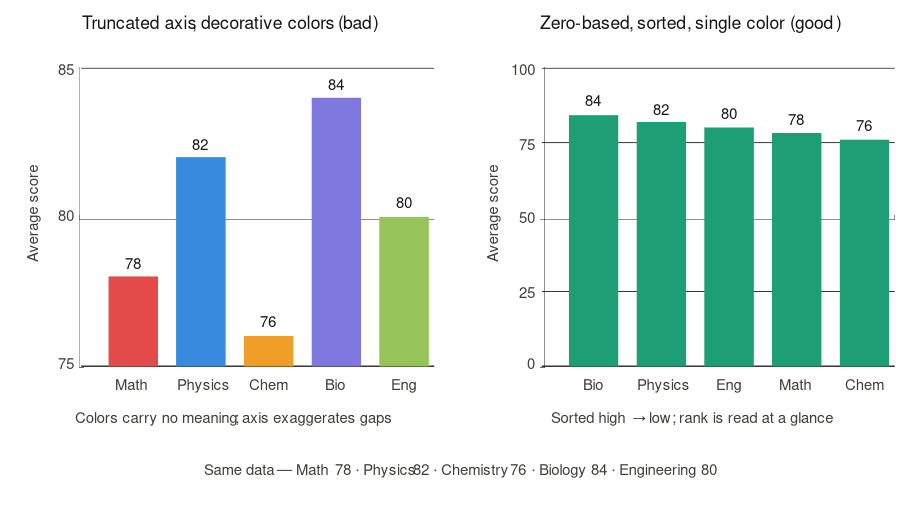
\includegraphics[width=0.85\linewidth]{slike/02/02-05.png}
    \caption{Стубичасти графикон просечних резултата испита по одељењима}
    \label{fig:02-2}
\end{figure}

Упркос својој једноставности, стубичасти графикони се често погрешно користе. Уобичајене грешке укључују скраћивање вертикалне осе, што преувеличава разлике, или примену стубичастих графикона на континуалне променљиве где би другачије визуелизације биле прикладније.

На Слици 2 се може видети пример лоше (лево) и добро (десно) дефинисаног стубичастог графа. На левом графикону је оса скраћена, чиме су разлике међу одељењима преувеличане, а ступци су поређани абецедно. Додатно, коришћене су различите боје (за сваки стубац) које не енкодирају никакве вредности (коришћене су само због естетике а не приказују податке). Због оваквог дизајна графа, читаоцу је потребно доста времена да добије одговоре на нека питања нпр: 

\begin{itemize}
  \item Који предмет има најбољу, а који најлошију просечну оцену?
  \item Која је разлика у поенима између најбољег и најлошије оцене на предметима?
\end{itemize}
На десном графикону оса почиње од нуле, а ступци су поређани по вредности, а боја свих стубаца је иста. На овај начин је поређење између предмета веродостојно приказано и омогућава једноставну и брзу анализу.

Ефективност стубичастог графикона зависи од малог броја дизајнерских одлука чија логика директно следи из перцептивне основе кодирања. Пошто дужина стубца носи квантитативно значење, сваки поступак који скреће пажњу са опажене дужине — скраћена основа, 3D аспеката (енг. \textbf{\textit{facet}}), почетак различит од нуле — искривљује и поређење које се од читаоца тражи. Додатно, редослед приказа значајно утиче на једноставност разумевања визуелизације: алфабетски редослед је прикладан само када сами називи носе аналитичку релевантност, док рангирање по вредности у први план ставља поређење које графикон и треба да подржи. Правила која следе консолидују ова разматрања у радну контролну листу:

\begin{itemize}
  \item Оса се започиње од нуле (величина се кодира дужином).
  \item Ступци се ређају по вредности (не абецедно), осим ако је редослед значајан.
  \item Хоризонтални ступци се користе за дугачке ознаке категорија.
  \item 3D приказ се избегава — њиме се искривљује перцепција дужине.
  \item Боја се користи само за кодирање друге променљиве, а не ради декорације.
\end{itemize}

\subsubsection{Анализа односа дела и целине}
Када аналитички задатак налаже приказ укупне вредности која разлаже на своје саставне компоненте, подаци се састоје од једне категоријалне променљиве чији нивои деле целину и квантитативне мере — типично збира или удела. Кружни графикон је најпознатији визуелни облик за овај задатак, кодирајући сваку компоненту као угаони исечак круга чија укупна површина представља целину. У пракси се овај графикон често назива и питичасти графикон, по узору на енглески термин \textbf{\textit{pie chart}}, који дословно значи „графикон у облику пите”. Графикон се интуитивно чита као композиција, а не као скуп независних величина, што представља његову главну аналитичку предност када су удели променљива од интереса.

\textbf{\textit{Пример:}} руководилац који прегледа структуру укупног прихода по линијама производа може користити кружни графикон да на први поглед прикаже које линије доминирају структуром, а које су маргиналне. Визуелни нагласак пада на релативне уделе, а не на апсолутне вредности, што је прикладно када се аналитичко питање односи на пропорционалност. Емпиријске студије графичке перцепције су ипак показале да су процене угла и површине знатно мање тачне од процена дужине дуж заједничке скале (Cleveland \& McGill, 1984), те је кружне графиконе најбоље резервисати за случајеве у којима је категорија мало, разлике између удела велике, а аналитичка порука квалитативна, а не квантитативна.

Када је потребно прецизно поређење удела, или када је број компоненти велики, пожељнији су алтернативни визуелни облици. Наслагани стубичасти графикони чувају тумачење дела и целине, а истовремено омогућавају тачније поређење засновано на дужини, и нарочито су ефективни када више целина треба поредити једну поред друге, као у структури прихода по регионима или кварталима.

\begin{figure}[h]
    \centering
    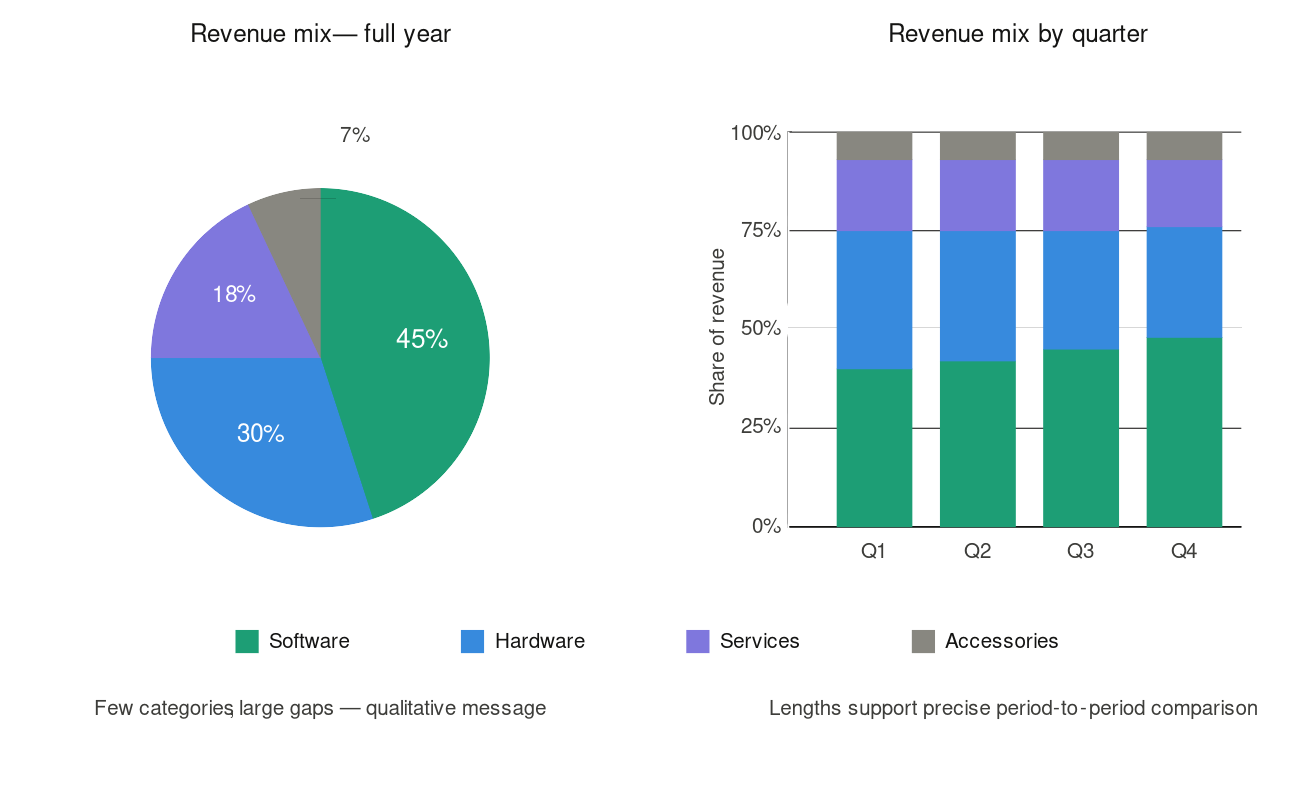
\includegraphics[width=0.85\linewidth]{slike/02/02-15.png}
    \caption{Кружни графикон и наслагани стубичасти графикон структуре прихода на нивоу целе године}
    \label{fig:02-3}
\end{figure}

Кружни графикон приказује поделу годишњег прихода — \textit{Software} доминира са 45\%, \textit{Accessories} је маргиналан са 7\% — што је типичан случај „мало категорија, велике разлике” у коме се кружни графикон тренутно чита (Слика~\ref{fig:02-3} лево). Наслагани стубичасти графикон десно узима исте четири линије производа и приказује њихов састав кроз Q1–Q4, тако да постепени раст \textit{Software}-а (40\% → 48\%) и компензациони пад \textit{Hardware}-а (35\% → 28\%) постају прецизно читљиви као разлике у дужини дуж заједничке основе (Слика~\ref{fig:02-3} десно).

\textbf{\textit{Мапе стабла}} (енг. \textit{treemap}) проширују исту логику на хијерархијске композиције, кодирајући угнежђене компоненте површином и омогућавајући смештај десетина категорија које би преоптеретиле кружни графикон. Уобичајене замке у свим приказима дела и целине укључују употребу тродимензионалних ефеката који искривљују перцепцију удела, укључивање категорија које заједно не исцрпљују целину и примену ових облика на податке који по својој природи нису истински композициони.

\begin{figure}[h]
    \centering
    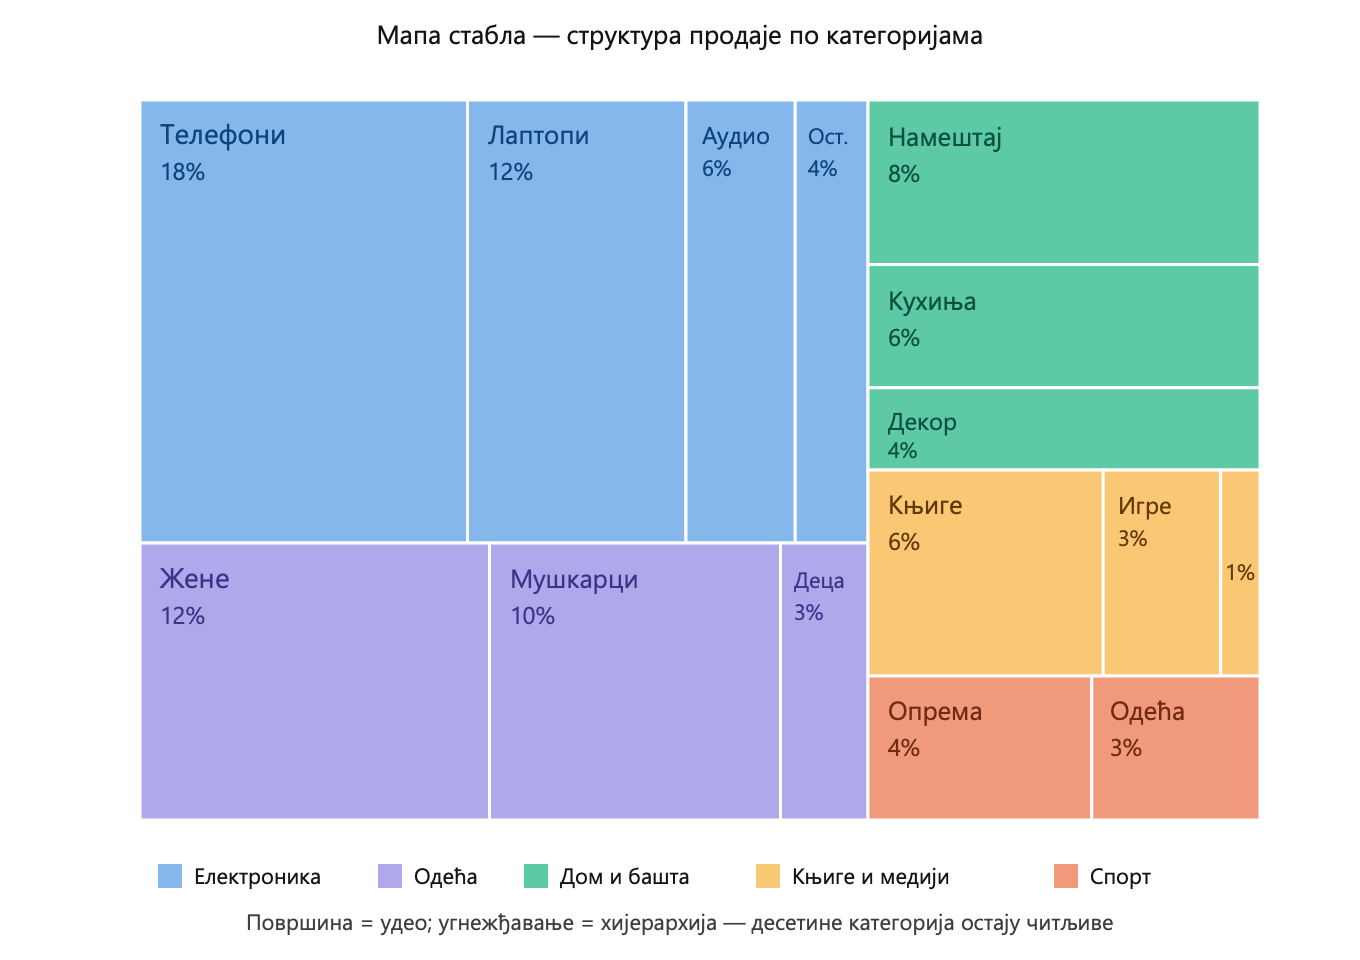
\includegraphics[width=0.85\linewidth]{slike/02/02-07.png}
    \caption{Мапа стабла}
    \label{fig:02-4}
\end{figure}

Мапа стабла приказује четрнаест подкатегорија продаје груписаних у пет главних категорија, при чему је површина сваког правоугаоника пропорционална уделу у укупној продаји. Електроника доминира са 40\% (Телефони сами носе 18\%), док мање категорије попут Музике (1\%) и даље остају видљиве — нешто што би на кружном графикону постало нечитљиво. Боја кодира главну категорију, а угнежђено распоређивање показује двослојну хијерархију без додатних осовина.

\subsubsection{Линијски и површински графикони}
Када су подаци индексирани временом, а аналитички циљ је идентификовати трендове, обрасце или временску промену, линијски графикони (енг. \textbf{\textit{Line charts}}) су најприкладнији визуелни облик. У овом случају, подаци се састоје од временске променљиве и квантитативне променљиве, при чему је време пресликано на хоризонтални положај (X-осу), а величина на вертикални положај (Y-осу).

Као илустративан пример, енергетски снабдевач који прати месечну потрошњу електричне енергије током више година може користити линијски графикон да открије сезонске флуктуације и дугорочни раст. Континуална природа линије појачава уређену структуру времена и омогућава посматрачима да уоче промене нагиба, које људи ефикасно тумаче као растуће или опадајуће трендове (Few, 2012). Линијски графикони постају проблематични када се примењују на неуређене категорије или када се истовремено прикаже превише линија, што доводи до визуелног нереда и интерпретативне двосмислености.

Близак сродник линијског графикона је површински графикон (енг. \textbf{\textit{Area chart}}), у коме је област између линије и хоризонталне осе попуњена како би се нагласила кумулативна величина, а не тренутна вредност. Површински графикони су погодни за комуницирање обима активности током времена — укупна продаја, укупна потрошња енергије, укупан улазни саобраћај — јер се попуњена површина чита као интеграл основне величине. Овај облик се природно проширује на наслагане површинске графиконе, који разлажу временски укупни износ на његове компонентне серије и комбинују тумачење дела и целине са временским, омогућавајући аналитичару да прати и еволуцију укупне величине и променљив састав њених делова. Површински графикони су ипак склони специфичним замкама: наслагане варијанте отежавају читање путање било које серије осим доње, јер свака горња серија лежи на флуктуирајућој основи, а преклапајући ненаслагани површински графикони заклањају појединачне серије услед оклузије. Зато су најделотворнији када је аналитички нагласак на агрегатној величини, а не на прецизном поређењу између компонентних серија.

\begin{figure}[h]
    \centering
    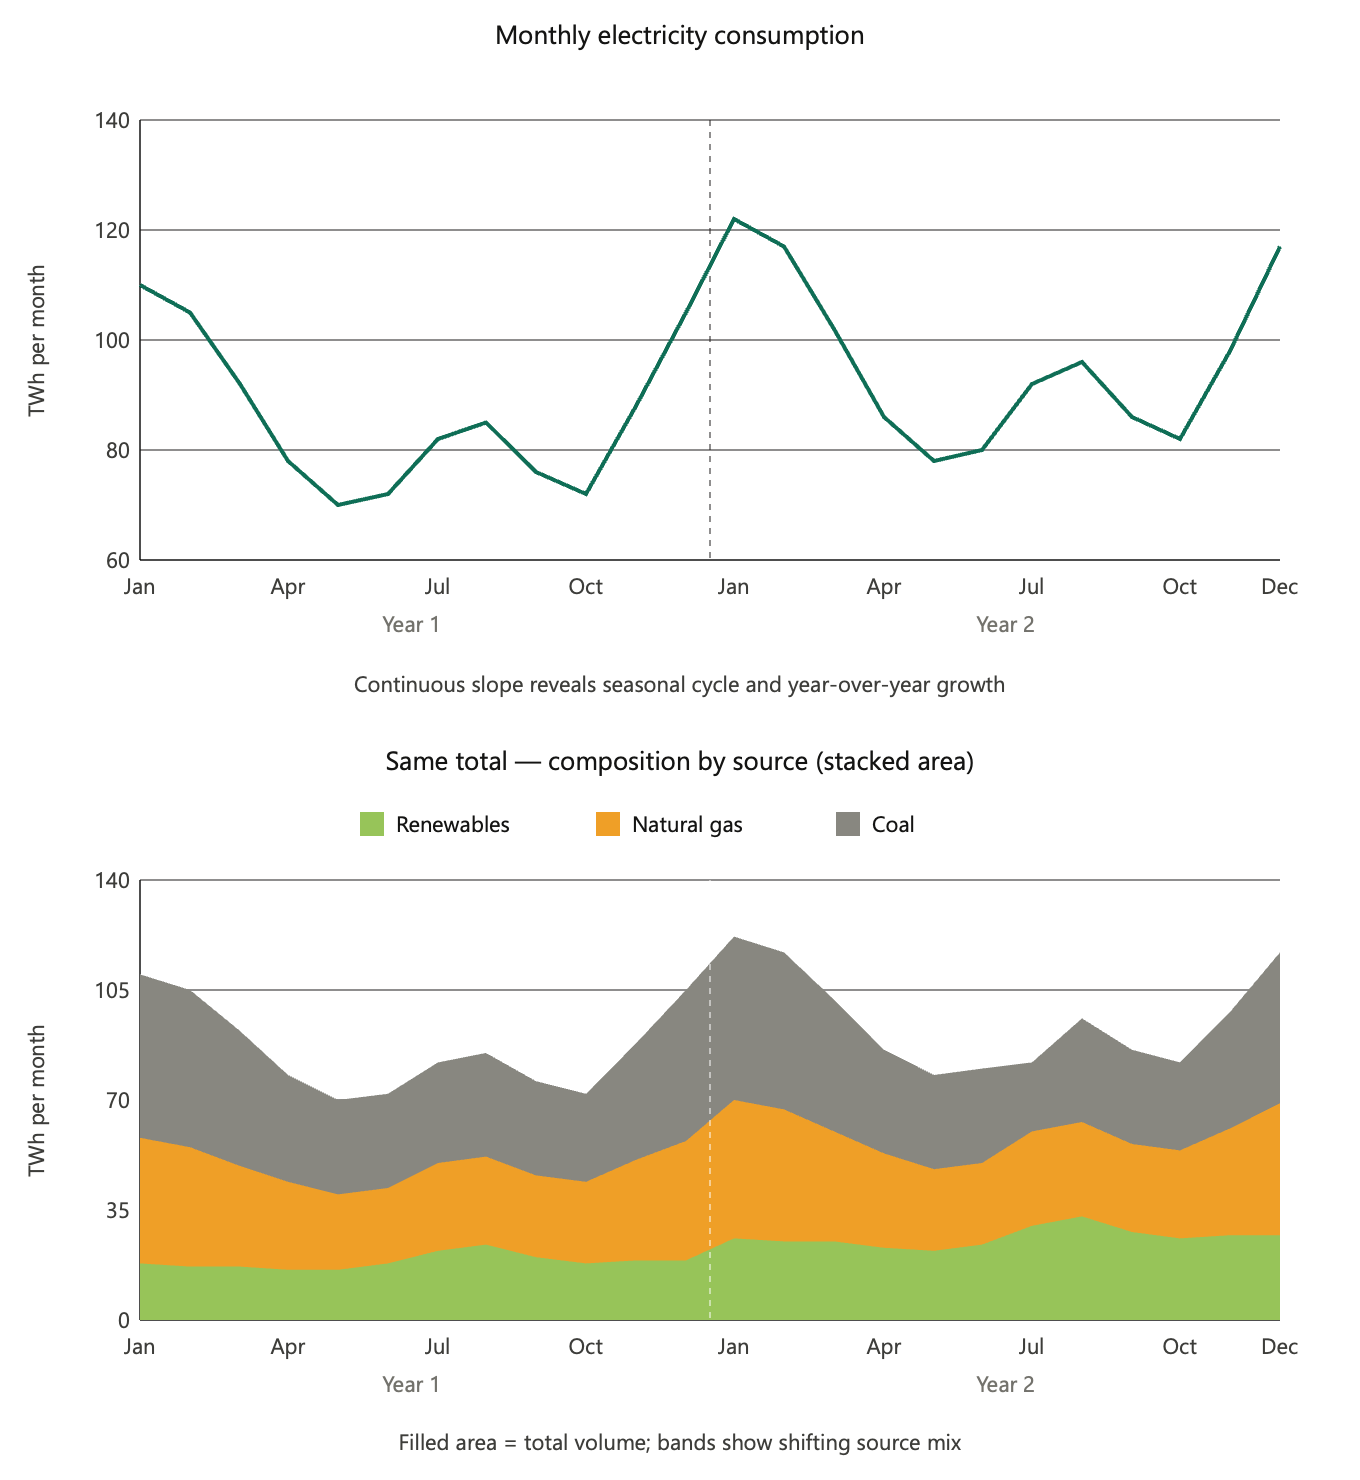
\includegraphics[width=0.85\linewidth]{slike/02/02-13.png}
    \caption{Линијски и површински графикон}
    \label{fig:02-5}
\end{figure}

Линијски графикон на врху приказује кретање укупне месечне потрошње електричне енергије кроз 24 месеца — кодирање нагибом чини сезонски циклус (зимски врхови у јануару, летњи падови у мају и јуну) и међугодишњи раст из прве у другу годину одмах читљивим као промене у смеру линије.

Површински графикон са слагањем испод приказује исте укупне вредности, али их разлаже на обновљиве изворе, природни гас и угаљ. Сада попуњене области преносе кумулативни обим — висина целог стека је укупна потрошња — док релативне дебљине трака показују да су обновљиви извори порасли (са око 18 на 30 TWh у зимским врховима), а да је учешће угља у истом периоду опало. То је двоструко читање које текст описује: временски тренд укупне вредности и промена у структури њених делова у једном кадру.

\subsubsection{Односи између променљивих}
Истраживање односа између нумеричких променљивих представља централни задатак у експлораторној анализи података, а „раштркани” дијаграми (енг. \textbf{\textit{Scatter plots}}) су посебно осмишљени за ту сврху. Раштркани дијаграм конструише се од две квантитативне променљиве, од којих је свака пресликана на једну од оса, док је свако опажање представљено као тачка у дводимензионалном простору.

Раштркани дијаграми могу бити обогаћени додатним кодирањима као што су боја или облик ради представљања категоричких груписања, али прекомерно украшавање може прикрити основну структуру података.

Читање раштрканог дијаграма почиње општим обликом „раштрканих” тачака. Ако се тачке у просеку подижу слева надесно, постоји позитивна корелација; ако се спуштају, корелација је негативна. Јачина везе не процењује се само по постојању нагиба, већ и по томе колико су тачке збијене око замишљеног тренда. Збијен и издужен облик указује на јаку повезаност (корелацију), док разливен облак указује на слабу. Овде је важно нагласити да раштркани дијаграм не служи само да покаже „има ли корелације”, већ и како је та повезаност обликована. Коначно, и када је образац јасан, мора се задржати основна методолошка опрезност: корелација није каузалност. Визуелизација открива да две променљиве иду заједно; она сама не доказује да једна узрокује другу.

Посебно је важно уочити нелинеарност. Многи односи у стварним подацима нису праволинијски: могу имати U-облик, праг након кога се промена убрзава, или ефекат засићења у коме даљи раст једне променљиве све мање прати раст друге. На пример, број сати учења и резултат на испиту могу бити позитивно повезани само до одређене тачке, после које додатно учење доноси све мањи добитак. Овакви закључци обично воде до додатних анализа и укључивања додатних променљивих (нпр. шта још утиче на коначну оцену: посета предавањима и вежбама, интеракција са наставним материјалима, концентрација приликом учења итд.). Управо зато визуелни преглед често открива нешто што једна једина корелациона мера не може да прикаже.

Раштркани дијаграм омогућава и уочавање кластера (група сличних података) и издвојених вредности. Кластери су важни јер могу указивати на постојање различитих подгрупа унутар истог скупа података, рецимо студената који редовно похађају наставу и оних који уче само пред испит. Издвојене вредности су подједнако значајне: оне могу бити грешке у уносу, али и случајеви од посебног аналитичког интереса. 

Раштркани дијаграм се често користи и за идентификацију екстремних вредности (енг. outliers) — тачака које значајно одступају од општег обрасца. Такве вредности се препознају као мали број изолованих тачака које су удаљене од главне масе података и подлежу додатној провери, јер могу указивати на грешку у мерењу, али и на ретке догађаје који носе важан аналитички сигнал.

\textbf{\textit{Пример:}} истраживач који испитује однос између времена проведеног у учењу и резултата на испиту може користити раштркани дијаграм да идентификује корелације, кластере сличног понашања или екстремне вредности (аутлајере). За разлику од агрегираних визуелизација, раштркани дијаграми чувају појединачна опажања, подржавајући генерисање хипотеза, а не њихову потврду (Tukey, 1977).

\begin{figure}[h]
    \centering
    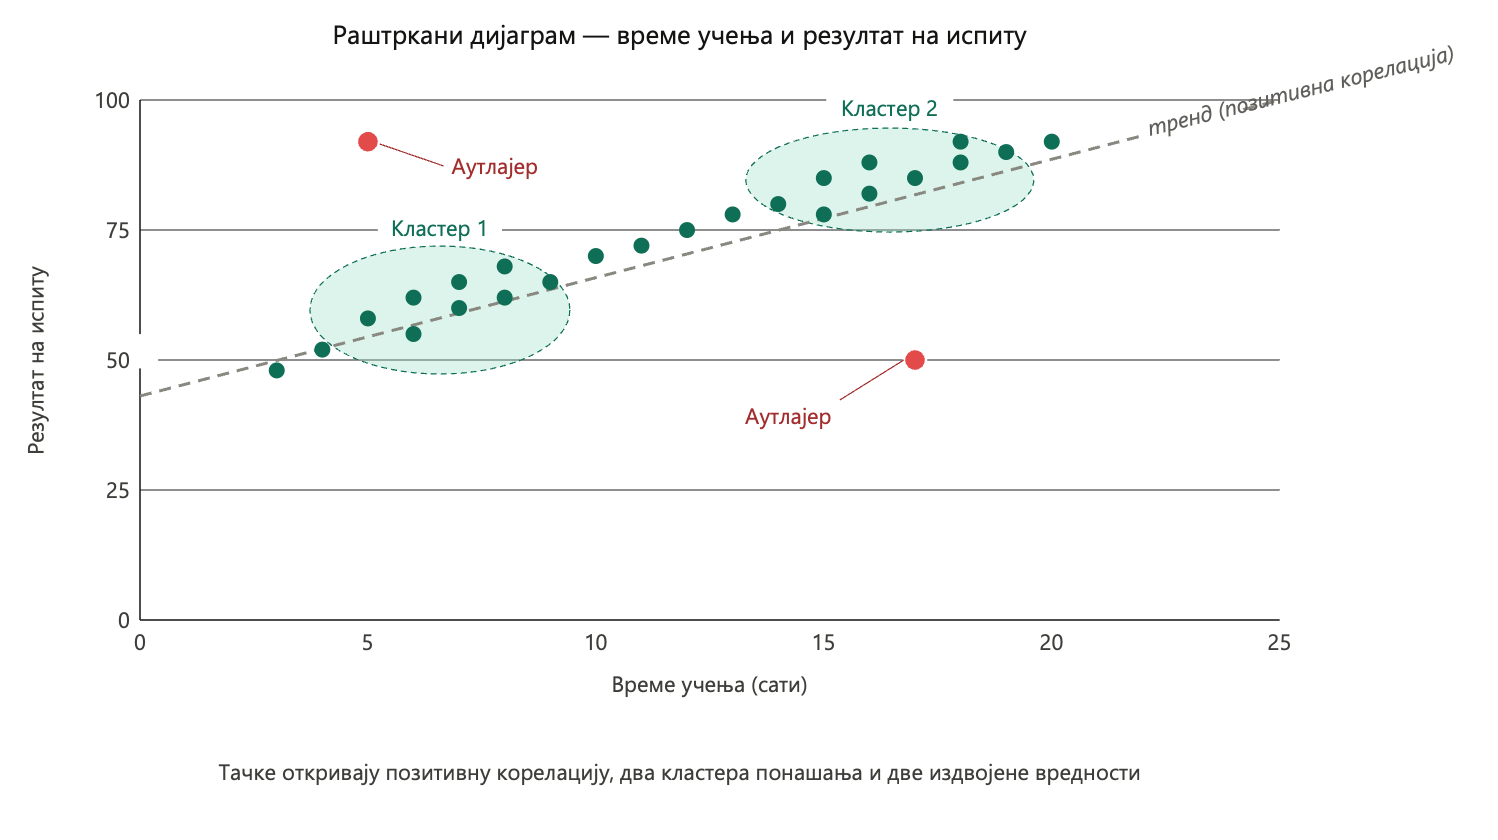
\includegraphics[width=0.85\linewidth]{slike/02/02-02.png}
    \caption{Раштркани дијаграм}
    \label{fig:02-6}
\end{figure}

Раштркани дијаграм истовремено показује сва три обрасца које текст наводи. Испрекидана сива линија тренда се пење с лева на десно — то је позитивна корелација између времена учења и резултата на испиту. Два светло осенчена овала истичу кластере сличног понашања: студенти са умереним учењем и умереним резултатима у доњем левом делу, и студенти са дуготрајним учењем и високим резултатима у горњем десном. Две црвене тачке означене као „Аутлајер“ одударају од општег обрасца — једна је ученик који је уложио мало времена али постигао одличан резултат, друга је ученик који је много учио али се ипак слабо снашао.

\subsubsection{Разумевање расподела}
Када се аналитички задатак помери са поређења или истраживања односа ка разумевању расподеле једне квантитативне променљиве, дистрибутивне визуелизације постају суштинске. Хистограми се конструишу дељењем квантитативне променљиве на интервале, односно делове (енг. \textbf{\textit{bins}}), и пребројавањем броја опажања у сваком од делова. Та структура омогућава аналитичарима да открију асиметрију, модалност и распон.

На пример, менаџер логистике који испитује времена испоруке може користити хистограм да утврди да ли су кашњења симетрична, десно искошена или обележена са више врхова. Такви увиди су кључни за избор одговарајућих статистичких модела и прагова перформанси (Wilkinson, 2005).

\textbf{\textit{Кутијасти дијаграми}} (енг. \textit{box plot}) нуде комплементаран приступ, посебно када се пореде расподеле међу категоријама. Они комбинују категоријалну променљиву са квантитативном променљивом, сумирајући сваку групу са пет канонских статистика: медијаном (централна линија у кутији, која означава 50. перцентил), првим и трећим квартилом (доња и горња ивица кутије, које означавају 25. и 75. перцентил), и „брковима”, који се по конвенцији протежу до најекстремнијих опажања унутар 1,5 пута интерквартилног распона (IQR = Q3 − Q1) од ивица кутије; опажања изван бркова приказују се појединачно као издвојене вредности. Сама кутија, дакле, визуелизује централних 50\% података (IQR), положај медијане унутар кутије открива асиметрију (медијана померена од центра сигнализира асиметричну расподелу), а издвојене вредности означавају опажања која заслужују појединачну пажњу уместо да буду утопљена у сумарну статистику. Поређење расподела плата по одељењима, на пример, постаје ефикасно и компактно коришћењем кутијастих дијаграма, нарочито када је укључено много категорија.

\begin{figure}[h]
    \centering
    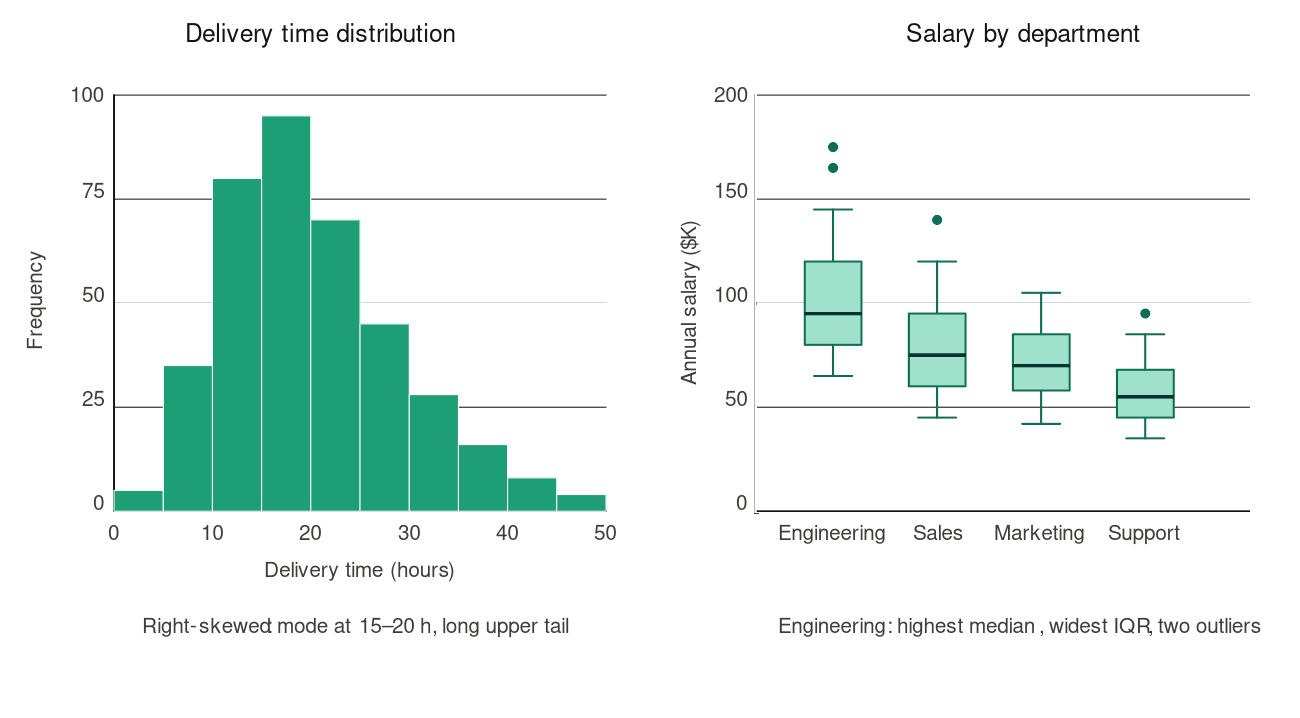
\includegraphics[width=0.85\linewidth]{slike/02/02-17.png}
    \caption{Хистограм времена испоруке и кутијасти дијаграм расподела плата по одељењима}
    \label{fig:02-7}
\end{figure}

Хистограм лево групише времена испоруке у интервале од 5 сати од 0 до 50 сати и приказује класичан десно искошен облик — већина испорука групише се око мода од 15–20 сати, са дугим репом спорих испорука које би менаџер логистике желео да испита. Кутијасти дијаграм десно сумира расподеле плата у четири одељења: свака кутија обухвата Q1 до Q3, тамна линија означава медијану, бркови се пружају до минимума и максимума унутар опсега, а тачке означавају издвојене вредности. Одељење Engineering има највишу медијану (\textasciitilde{}\$95K), најшири интерквартилни распон и две високе издвојене вредности, док је Support најниже и најуже — управо она врста међукатегоријалног поређења коју би било тешко читати из четири одвојена хистограма.

\subsubsection{Матрични подаци и топлотне мапе}
Одређени скупови података природно формирају матричну структуру, где су вредности индексиране двема категоричким или ординалним димензијама. У таквим случајевима, топлотне мапе пружају компактну и ефективну визуелизацију кодирајући вредности интензитетом боје. Конструкција укључује две дискретне променљиве пресликане на положај и једну квантитативну променљиву пресликану на боју.

Типичан пример је анализа саобраћаја на веб-сајту по сату у дану и дану у недељи. Топлотна мапа (енг. \textbf{\textit{Heatmap}}) може одмах открити периоде вршног коришћења кроз тамније области боје. Њена главна предност је у томе што брзо открива образац. Њено ограничење је што боја није добар начин за прецизно читање бројева. Зато је топлотна мапа одлична када желимо да уочимо где је нешто израженије, а мање погодна када желимо да тачно упоредимо мале разлике између вредности.

\begin{figure}[h]
    \centering
    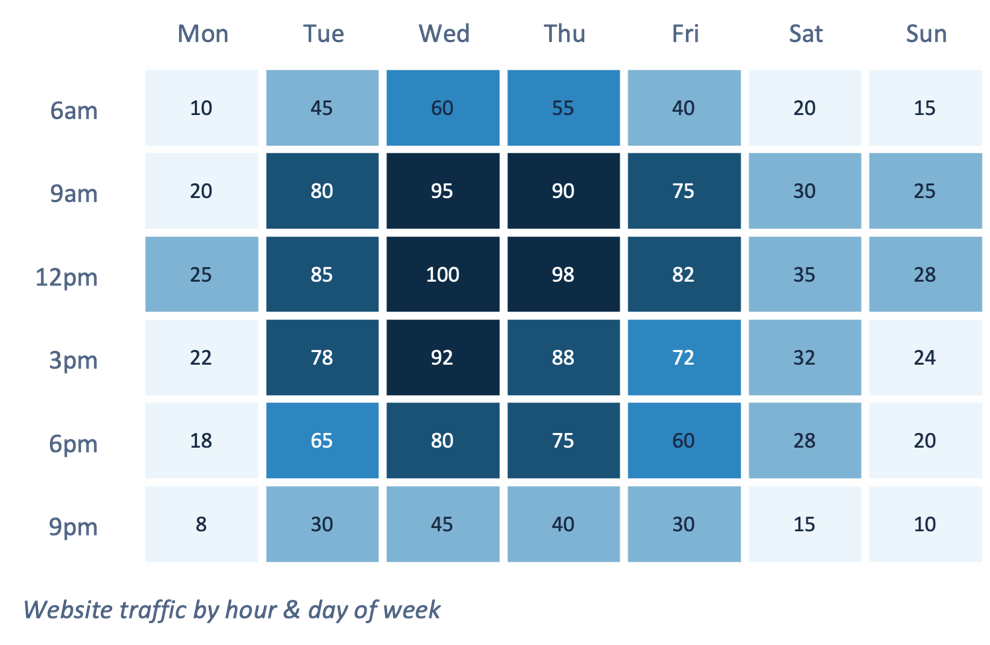
\includegraphics[width=0.85\linewidth]{slike/02/02-30.png}
    \caption{Топлотна мапа саобраћаја на веб-сајту по сату у дану и дану у недељи, која кроз интензитет боје открива периоде вршног коришћења}
    \label{fig:02-8}
\end{figure}

Топлотна мапа наслеђује и предности и ограничења утврђена у ранијим одељцима. Попут стубичастих и линијских графикона из §2.1.4, кодирање је принципијелно, а не декоративно — боја носи квантитативно значење, и сваки поступак који искривљује опажену боју искривљује и поређење. Али тамо где кодирања заснована на дужини припадају перцептивно најпоузданијем врху хијерархије графичке перцепције (Cleveland \& McGill, 1984) (§2.1.5), засићеност боје налази се знатно ниже на тој лествици: посматрачи могу рангирати интензитете боје, али из њих не могу очитати прецизне вредности. Топлотна мапа је, дакле, алат за откривање образаца — кластера, периодичности, асиметрије по матрици — а не за подршку фином квантитативном поређењу. Дизајнерска правила која следе практичне су последице овог перцептивног ограничења: избори који чувају рангирање вредности, а да притом не подстичу читаоца да доноси прецизне квантитативне судове које само кодирање не може поуздано да подржи.

Правила дизајна топлотне мапе:

\begin{itemize}
  \item Користите перцептивно уједначене скале боја (нпр. viridis)
  \item Избегавајте rainbow колор-мапе — искривљују величину
  \item \textbf{\textit{Нормализујте вредности пре поређења}}
\end{itemize}

\subsubsection{Просторни контекст и географске карте}
Када су подаци географски, просторне визуелизације као што су карте постају незаменљиве. Карте кодирају просторне променљиве кроз положај и често представљају квантитативне атрибуте помоћу боје или величине. Аналитичар јавног здравља који мапира стопе инфекције по регионима може брзо идентификовати просторне неједнакости употребом хороплет карте (енг. \textbf{\textit{choropleth map}}), под условом да су вредности адекватно нормализоване.

\begin{figure}[h]
    \centering
    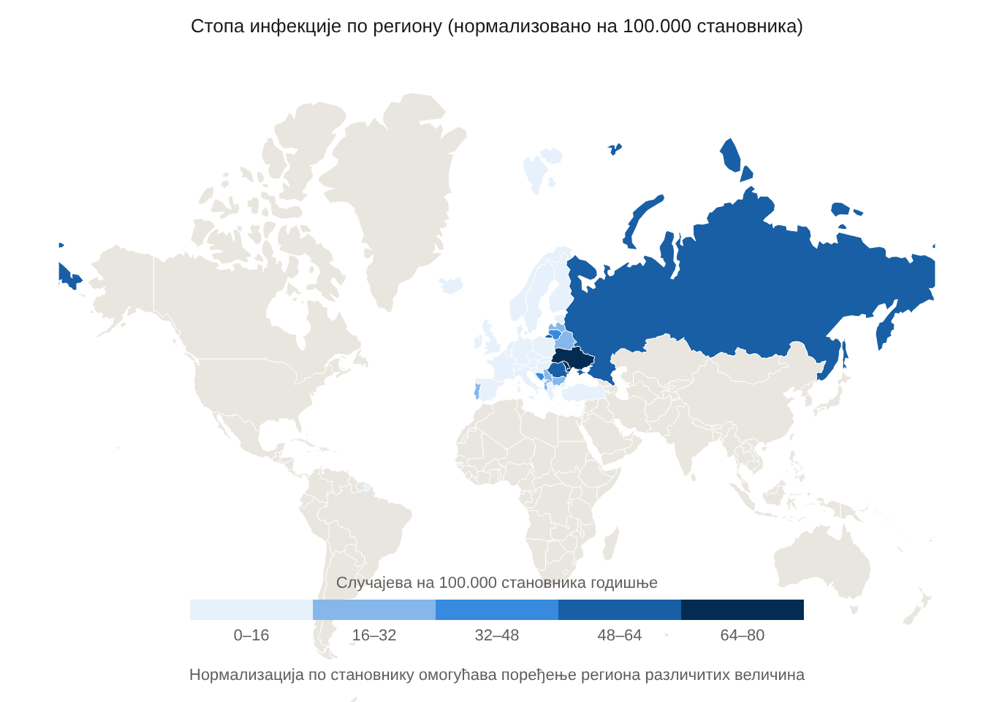
\includegraphics[width=0.85\linewidth]{slike/02/02-18.png}
    \caption{Хороплет карта стопе инфекције по регионима (случајеви на 100.000 становника), где нијанса боје кодира интензитет појаве и омогућава просторно поређење региона}
    \label{fig:02-9}
\end{figure}

Карте треба користити само када су просторни односи аналитички значајни. Коришћење карте за приказ непросторних поређења уводи непотребну сложеност и носи ризик од обмањујућег тумачења (Slocum et al., 2009).

Другим речима, карта има смисла онда када је питање по природи географско: где је проблем концентрисан, да ли постоји просторни кластер, да ли се појава шири дуж коридора, границе или урбане осе. Ако менаџера интересује само поређење укупне продаје по регионима, а географски положај региона није важан за тумачење, стубичасти графикон је обично бољи избор, јер омогућава прецизније поређење дужина него што карта омогућава поређење нијанси и површина. Карта је супериорна тек онда када позиција сама носи део значења.

Нормализација је кључна код хороплет карата. Ако се региони обоје по апсолутном броју становника, случајева болести или продаја, већи и насељенији региони ће скоро увек изгледати „важније”, чак и када је њихова стопа по становнику умерена. Зато се често приказују стопе по 1.000 или 100.000 становника, приход по купцу или број инцидената по квадратном километру. Таква нормализација омогућава фер поређење јединица различите величине. Без ње карта меша два различита питања: колико нечега има укупно и колико је појава интензивна у односу на величину популације или подручја.

Проблем постаје још израженији зато што површина региона визуелно може да завара. Велики, ретко насељени региони заузимају много простора на карти и природно привлаче пажњу посматрача, док мали, густо насељени урбани региони могу остати у другом плану иако су аналитички значајнији. Зато је добра пракса да карта буде допуњена стубичастим графиконом или табелом ранга: карта даје просторни контекст, а графикон омогућава прецизно поређење.

\subsubsection{Визуелизација неизвесности и варијабилности}
У многим аналитичким контекстима, централна тенденција података је мање информативна од њихове варијабилности и неизвесности. Игнорисање неизвесности може довести до претерано самоуверених закључака и погрешног доношења одлука, нарочито у областима као што су прогнозирање, процена ризика и анализа политика.

Неизвесност може настати услед варијабилности узорковања, грешке мерења или претпоставки модела. Визуелизација игра кључну улогу у транспарентном саопштавању ових аспеката. Традиционалне тачкасте процене, када се приказују без контекста, имплицирају лажан осећај прецизности.

На пример, ако је потребно приказати прогнозу потражње за наредни квартал, једна линија није довољна. Корисно је показати и распон у коме се стварни исход може кретати, јер тако читалац не види само очекивани тренд, већ и колико је прогноза сигурна.

Овде је важно јасно раздвојити варијабилност података од неизвесности процене. Варијабилност података означава да се сама појава природно мења од случаја до случаја: потрошња купаца, време испоруке или температура заиста варирају и када не постоји никаква грешка мерења. Неизвесност процене означава нешто друго: колико смо сигурни у неку сумарну величину или параметар који процењујемо на основу ограниченог броја опажања, на пример у просечну потражњу или у нагиб тренда. То су, дакле, два различита извора „распршености” и не смеју се тумачити као исто.

\textbf{\textit{Пример}}. Ако се посматра потрошња 100 домаћинстава, распон њихових појединачних вредности показује колико се домаћинства заиста разликују. Ако се израчуна просек и око њега се прикаже интервал поверења, тај интервал говори колико је процена просека сигурна. Ако се прикаже предиктивни интервал, онда је потребно показати у ком распону може пасти неко будуће појединачно опажање. Зато визуелизација неизвесности мора јасно да каже шта тачно приказује: варијабилност самих података, неизвесност процене или неизвесност прогнозе.

\begin{figure}[h]
    \centering
    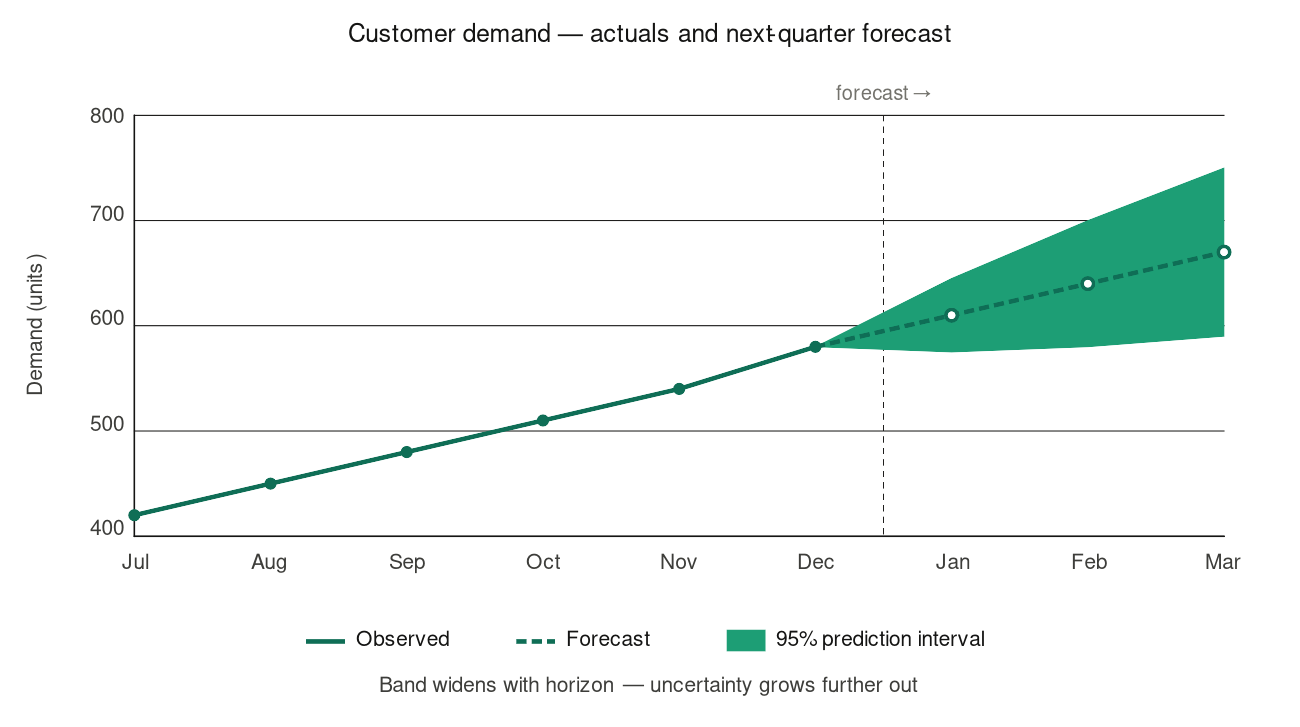
\includegraphics[width=0.85\linewidth]{slike/02/02-22.png}
    \caption{Линијски графикон са појасевима неизвесности око прогнозног тренда}
    \label{fig:02-10}
\end{figure}

Графикон приказује шест месеци посматране потражње купаца као пуну линију која расте од 420 до 580 јединица, а затим на испрекиданом вертикалном маркеру прелази у тромесечну прогнозу (610, 640, 670 јединица) исцртану испрекиданом линијом са шупљим маркерима. Засенчени тиркизни појас око прогнозе представља 95\% предиктивни интервал — узак на месту прелаза са посматраних података и све шири са хоризонтом, тако да посматрач не види само очекивану путању већ и колико је та путања поуздана у свакој тачки.

Кутијасти дијаграми нуде још један ефективан механизам за представљање варијабилности, нарочито при поређењу расподела међу групама. Када се пореде времена испоруке по логистичким провајдерима, кутијасти дијаграм открива не само просечне перформансе већ и доследност и издвојене вредности — факторе који су често релевантнији за оперативне одлуке.

\begin{figure}[h]
    \centering
    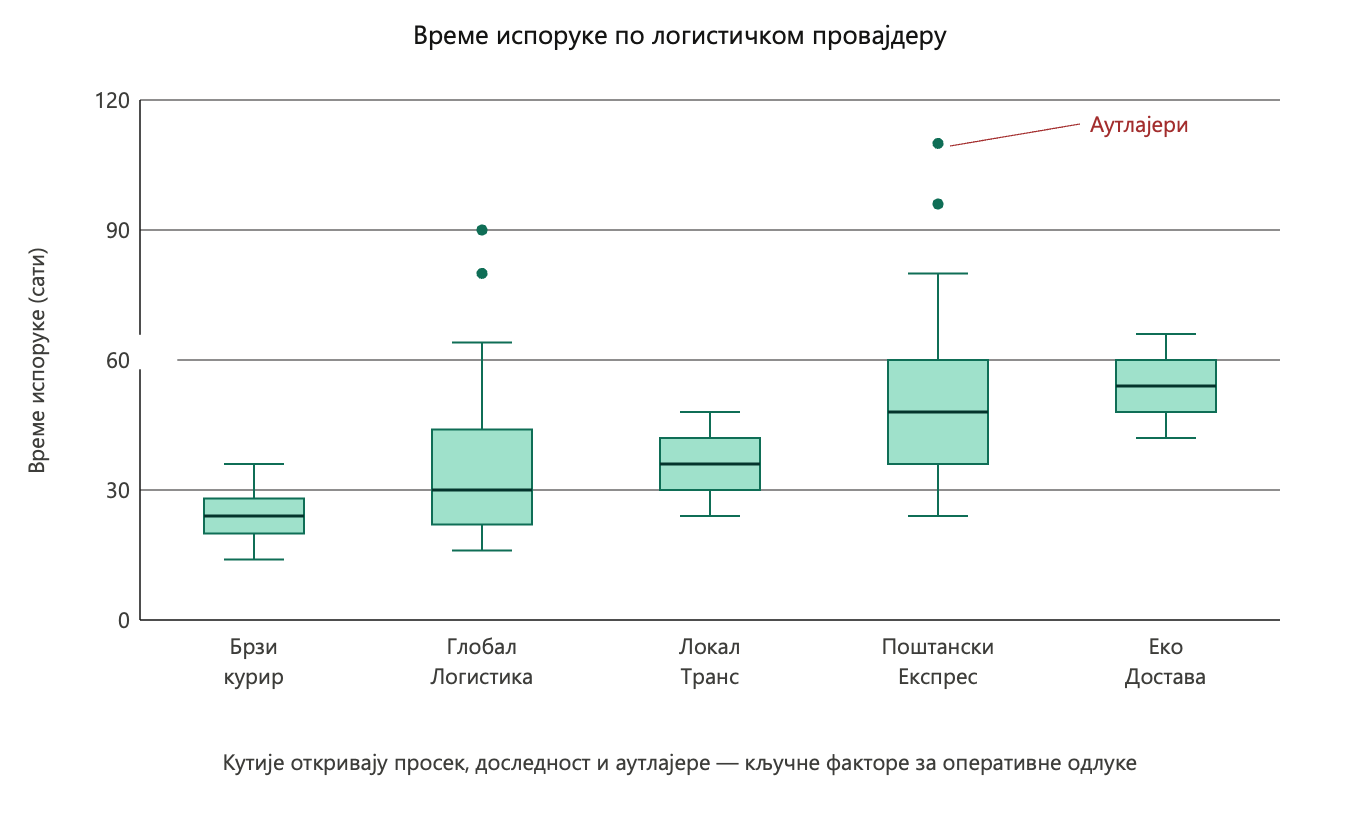
\includegraphics[width=0.85\linewidth]{slike/02/02-20.png}
    \caption{Кутијасти дијаграм времена испоруке по логистичким провајдерима — медијана, интерквартилни распон и издвојене вредности омогућавају истовремено поређење просечних перформанси, доследности и екстремних случајева међу групама}
    \label{fig:02-11}
\end{figure}

Уобичајене грешке у визуелизацији неизвесности укључују коришћење линија грешке (енг. \textbf{\textit{error bar}}) без објашњења, примену симетричних интервала на искошене расподеле или потпуно изостављање неизвесности. Такве праксе крше принцип да визуелизација треба да подржи поштену инференцију, а не само уверљиву презентацију (Tufte, 2001).

\subsection{Визуелно кодирање}
Еволуција праксе визуелизације снажно је обликована теоријским истраживањима о томе како људи опажају и тумаче визуелне информације. Кључан допринос у овој области дали су (Cleveland \& McGill, 1984), који су обезбедили емпиријску основу за графичку перцепцију. Њихов експериментални рад показао је да се различита визуелна кодирања значајно разликују по тачности када се користе за квантитативне процене (Cleveland \& McGill, 1984).

\begin{figure}[h]
    \centering
    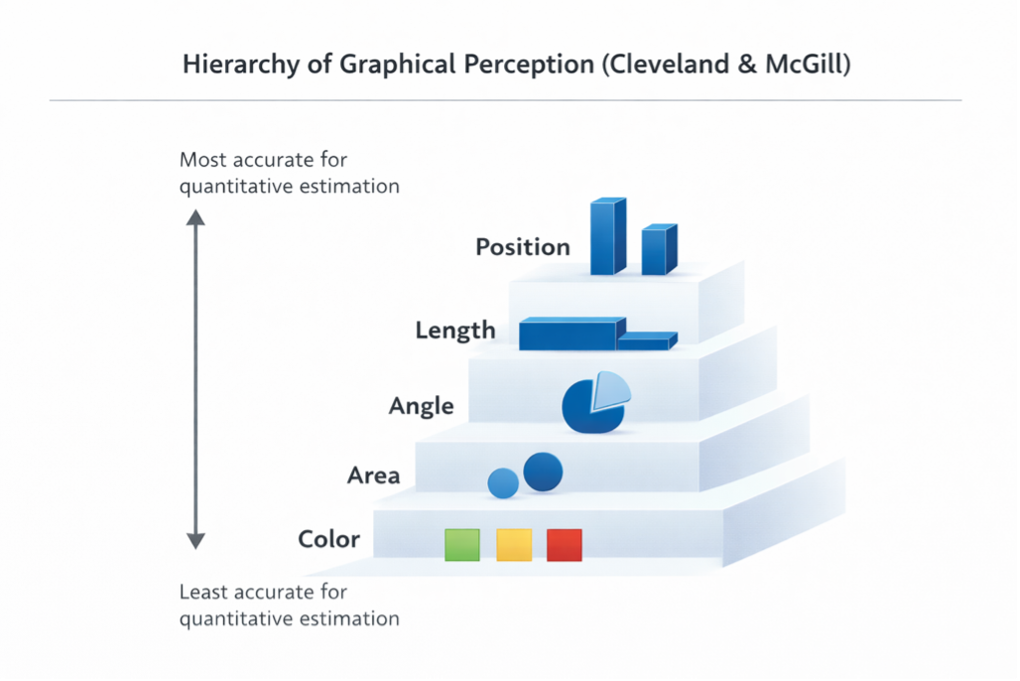
\includegraphics[width=0.85\linewidth]{slike/02/02-24.png}
    \caption{Хијерархија графичке перцепције (Cleveland \& McGill, 1984)}
    \label{fig:02-12}
\end{figure}

Истраживања показују да су прикази засновани на положају дуж исте скале тачнији за читање од приказа заснованих на дужини, углу, површини или боји. Зато су, на пример, дијаграми расејања и стубичасти графикони по правилу погоднији од кружних графикона када желимо прецизно поређење вредности.

Едвард Туфте је овај поглед допунио једноставним правилом: графикон треба да носи што више информације, а што мање сувишне декорације. Његов познати концепт односа мастила и података (енг. \textbf{\textit{data-ink ratio}}) управо то наглашава: треба смањити елементе који лепо изгледају, али не помажу разумевању (Tufte, 2001).

\begin{figure}[h]
    \centering
    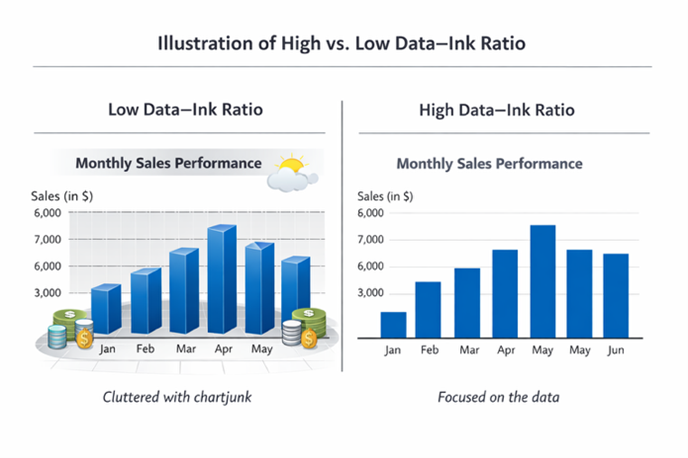
\includegraphics[width=0.85\linewidth]{slike/02/02-27.png}
    \caption{Поређење високог и ниског data–ink односа у дизајну графикона}
    \label{fig:02-13}
\end{figure}

Практичари додатно упозоравају на проблем визуелног нереда. Када графикон има превише боја, сувишних облика, анотација и декоративних линија, корисник теже уочава оно што је заиста важно. Пажња се распршује, читање постаје напорно, а образац који је потребно приказати остаје у другом плану. Зато добра визуелизација јасно истиче најважније елементе и не затрпава приказ непотребним детаљима (Few, 2012).

Ова три принципа се лако виде у пракси. Ако менаџер пореди квартални приход по пословним јединицама, стубичасти графикон ће му омогућити да разлике одмах уочи. Ако исте податке прикажемо кружним графиконом, корисник мора да процењује углове, што је мање поуздано. Ако томе додамо 3D ефекте, сенке и непотребну легенду, читање постаје још теже. У таквим случајевима графикон изгледа сложеније, а говори мање (Tufte, 2001). Зато једноставан, јасно организован графикон најчешће пружа најбољи увид.

\subsection{Вишедимензионални прикази}
Проблеми из стварног света ретко се своде на једну променљиву. Најчешће је потребно посматрати више атрибута истовремено: време, регион, производ, категорију купца, цену, количину и слично. Зато је задатак визуелизације вишедимензионалних података да помогне кориснику да у таквој сложености ипак уочи поређења, трендове и важне обрасце.

За разлику од једноставнијих приказа, овде циљ није да све променљиве „стану” у један графикон. Много је важније да се подаци паметно поделе на више повезаних приказа који омогућавају јасно поређење и постепено разумевање (Cleveland, 1993; Few, 2012).

\subsubsection{Мали вишеструки прикази}
\textbf{\textit{Мали вишеструки прикази}} (енг. \textit{small multiples}) су једна од најпрактичнијих техника за рад са вишедимензионалним подацима. Уместо једног претрпаног графикона, прави се низ сличних графикона, при чему сваки приказује један подскуп података, али са истим скалама и истим начином приказивања (Tufte, 1990).

Суштина је једноставна: ако су сви панели нацртани на исти начин, корисник ће разлике које види тумачити као разлике у подацима, а не као разлике у дизајну. Тако се поређење убрзава и читање постаје лакше.

Размотримо приход од продаје мерен током времена за више географских региона. Уместо да се сви региони прикажу у једном вишелинијском графикону — где се линије могу преклапати и постати тешко разлучиве — сваки регион може бити приказан у засебном линијском графикону распоређеном у мрежу. Време је представљено на x-оси, а приход на y-оси у сваком панелу.

\begin{figure}[h]
    \centering
    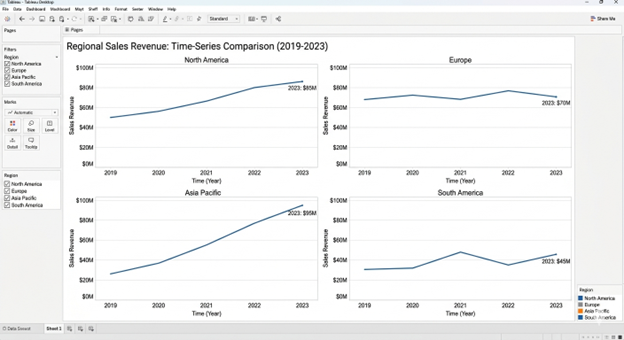
\includegraphics[width=0.85\linewidth]{slike/02/02-23.png}
    \caption{Мали вишеструки прикази (енг. small multiples) временских линијских графикона који приказују приход од продаје по регионима, уз доследне осе и скале}
    \label{fig:02-14}
\end{figure}

Ова техника најчешће укључује:

\begin{itemize}
  \item једну континуалну или временску променљиву (x-оса),
  \item \textbf{\textit{једну квантитативну меру (y-оса),}}
  \item једну категоријалну димензију која се користи за поделу података.
\end{itemize}
Мали вишеструки прикази су посебно корисни када желимо да видимо трендове, сезонске обрасце и одступања по категоријама, а да при томе не дође до преклапања елемената у једном графикону (енг. \textbf{\textit{overplotting}}). Зато се користе и када истражујемо податке и када желимо да резултат јасно објаснимо другима (Tufte, 1990; Wilke, 2019).

\subsubsection{Решеткасти прикази података}
\textbf{\textit{Фацетирање}} (енг. \textit{faceting}), односно решеткасти прикази (енг. \textit{trellis plots, lattice graphics}), проширује идеју малих вишеструких приказа тако што податке дели по једној или више категоричких димензија. Свака комбинација вредности добија свој панел, а у сваком панелу остаје исти тип графикона.

Ову технику је у статистичкој графици формализовао Cleveland (1993), а нарочито је корисна када је потребно видети како се односи у подацима мењају кроз више категорија.

Претпоставимо да се резултати задовољства купаца анализирају по категоријама производа и сегментима купаца током времена. Фацетирани распоред може поставити категорије производа у редове, а сегменте купаца у колоне, при чему сваки панел приказује временску серију оцена задовољства.

\begin{figure}[h]
    \centering
    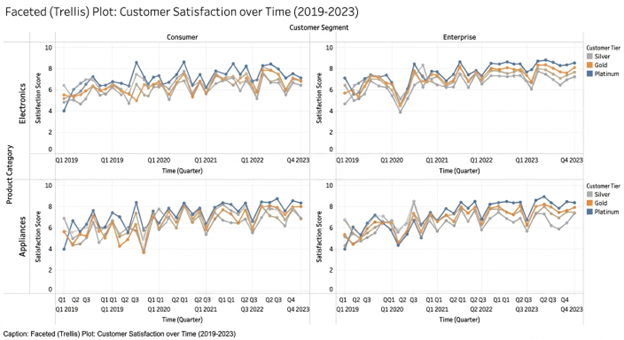
\includegraphics[width=0.85\linewidth]{slike/02/02-31.png}
    \caption{Фацетирани (енг. trellis) графикон задовољства купаца током времена, распоређен по категорији производа (редови) и сегменту купаца (колоне)}
    \label{fig:02-15}
\end{figure}

Фацетирање најчешће укључује:

\begin{itemize}
  \item једну или две категоријалне променљиве које се користе за распоред панела,
  \item једну или више квантитативних променљивих приказаних унутар панела,
  \item фиксно графичко кодирање које се понавља кроз све панеле.
\end{itemize}
Савремени алати као што су Tableau и ggplot2 третирају фацетирање као основну технику, јер омогућава да се сложени подаци прикажу прегледно и без губитка јасноће (Few, 2012; Munzner, 2014).

\subsubsection{Изазови визуелизације високодимензионалних података}
Ипак, ни мали вишеструки прикази ни фацетирање не решавају све проблеме. Када број димензија превише порасте, расте и ризик да приказ постане претрпан или да корисник погрешно протумачи оно што види.

Основно ограничење је у томе што људи могу поуздано да прочитају само ограничен број визуелних канала, а положај и дужина су и даље много прецизнији од боје или облика (Cleveland \& McGill, 1984).

Изазови визуелизације високодимензионалних података најчешће укључују:

\begin{itemize}
  \item \textbf{\textit{преклапање исцртаних елемената}} (енг. \textit{overplotting}),
  \item смањену интерпретабилност сложених кодирања,
  \item тешкоћу очувања смислених односа растојања.
\end{itemize}
Зато се у пракси често користе:

\begin{itemize}
  \item технике смањења димензионалности (нпр. Анализа главних компонената) пре визуелизације,
  \item интерактивне механизме као што су филтрирање, означавање избора (енг. \textit{brushing}) и увећавање приказа (енг. \textit{zooming}),
  \item повезане приказе, где више координисаних графикона заједно представља различите пројекције истих података.
\end{itemize}
У контролним таблама овакви подаци најбоље функционишу када се сложеност открива постепено, кроз интеракцију. Корисник прво види општу слику, а затим по потреби улази дубље. Зато су интеракција и координисани прикази важан део савремене визуелне аналитике (Few, 2013; Munzner, 2014). Технике интеракције и израде контролних табли биће описане у §§2.1.8 и 2.1.9 и Одељку 6.

\subsection{Приповедање}
\textbf{\textit{Приповедање помоћу података}} (енг. \textit{storytelling with data}) подразумева представљање резултата анализе података тако да публика разуме шта је важно и зашто је то важно. За разлику од експлораторне визуелизације, где корисник слободно истражује податке, овде је нагласак на јасној комуникацији и вођењу публике ка одређеном увиду, тумачењу или препоруци (Segel \& Heer, 2010; Knaflic, 2015).

Основа доброг приповедања помоћу података је јасна наративна структура. Она публици помаже да прати ток приче, разуме податке и запамти главни закључак. У пракси, већина оваквих прича прати једноставан редослед: контекст, развој проблема, кључни увид и последица или препорука (Kosara \& Mackinlay, 2013).

Често прихваћен оквир укључује следеће компоненте:

\begin{itemize}
  \item \textbf{\textit{Контекст и мотивација}}: Увођење домена проблема, аналитичког питања и релевантности података.
  \item \textbf{\textit{Аналитичка тензија}}: Представљање кључних поређења, трендова или аномалија који отварају питања или откривају неизвесност.
  \item \textbf{\textit{Разрешење и увид}}: Истицање централних аналитичких налаза изведених из података.
  \item \textbf{\textit{Импликације и акција}}: Повезивање увида са одлукама, препорукама или стратешким поступцима.
\end{itemize}
Суштина је да визуелизација не треба само да покаже податке, већ и да помогне публици да дође до исправног закључка (Tufte, 2001). У пословној интелигенцији и контролним таблама (које ће бити објашњене у каснијем тексту) то се често постиже пажљивим редоследом приказа, постепеним откривањем детаља и јасним повезивањем са кључним показатељима перформанси (енг. \textbf{\textit{key performance indicators}}, KPI) (Few, 2013). Важно је напоменути да приповедање на основу података није обавезно везано за контролне табле већ и за појединачне визуелизације. 

Основне технике које се користе у приповедању на основу података су: \textbf{\textit{анотација}} и \textbf{\textit{контекстуализација}}. Анотација и контекстуализација помажу да се значење угради директно у графикон. И када је приказ добро дизајниран, кратак текстуални сигнал често помаже кориснику да одмах разуме шта треба да примети и зашто је то важно (Knaflic, 2015).

Анотације могу укључивати:

\begin{itemize}
  \item Дескриптивне ознаке које идентификују критичне вредности или догађаје.
  \item Објашњавајуће напомене које разјашњавају трендове, аномалије или прекиде у обрасцима.
  \item Контекстуалне маркере који повезују тачке података са спољним догађајима, променама политика или пословним одлукама.
\end{itemize}

\begin{figure}[h]
    \centering
    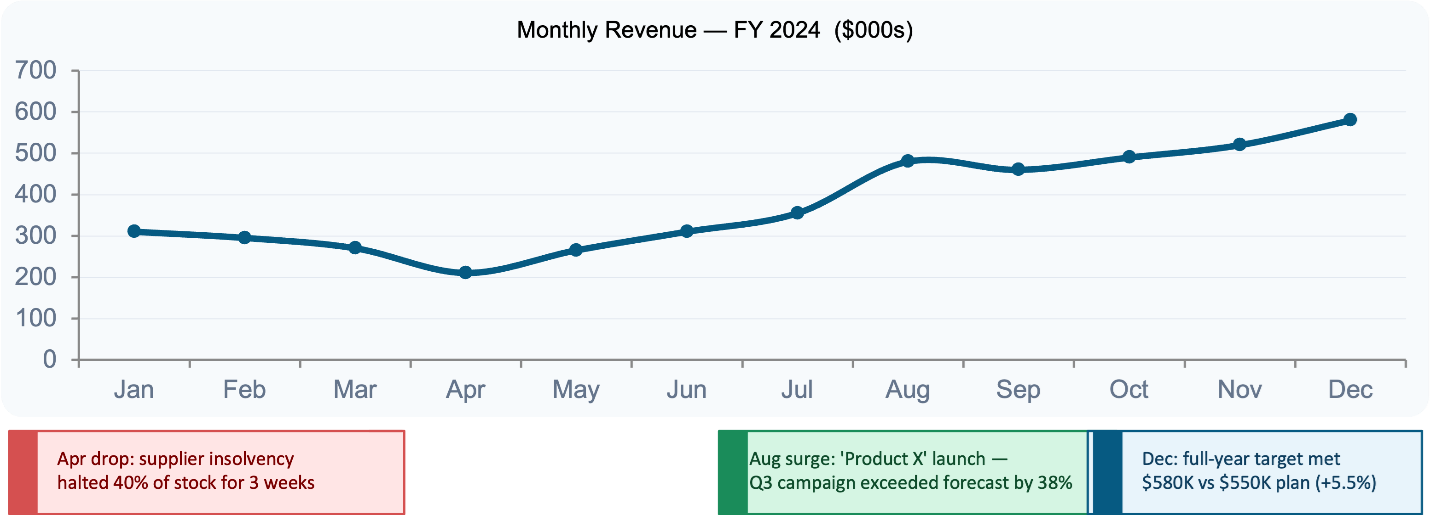
\includegraphics[width=0.85\linewidth]{slike/02/02-21.png}
    \caption{Анотирани графикон који повезује уочене обрасце са пословним догађајима}
    \label{fig:02-16}
\end{figure}

На слици су анотацијама истакнути кључни тренутни догађаји који објашњавају скокове и падове у временској серији. Текстуалне ознаке су повезане са одговарајућим тачкама на графикону, чиме је читаоцу омогућено да уочене обрасце директно повеже са пословним контекстом, без посебне референце на додатну табелу или текст.

Истраживања графичке перцепције показују да људи не изводе сами увек исти закључак само на основу обрасца који виде (Cleveland \& McGill, 1984). Зато анотације имају важну улогу: оне усмеравају пажњу и помажу да се визуелни образац повеже са правилним тумачењем. То је посебно важно када се на основу графикона доносе озбиљне пословне одлуке.

\subsection{Интеракција над визуелизацијама}
Технике интеракције су кључни део савремених система за визуелизацију и визуелну аналитику. За разлику од статичких приказа, интерактивна визуелизација омогућава кориснику да мења поглед на податке, пореди различите перспективе и постепено проверава своје претпоставке. Тако визуелизација постаје радни простор за размишљање, а не само средство приказивања резултата (Card, Mackinlay, \& Shneiderman, 1999; Keim et al., 2008).

Интеракција у пракси помаже кориснику да мање памти, а више проверава хипотезе директно на приказу (Ware, 2013). У алатима као што су \textit{Tableau}, \textit{Power BI} и веб-засноване контролне табле, филтрирање, означавање избора (енг. \textit{brushing}), увећавање приказа (енг. \textit{zooming}), продубљивање увида (енг. \textit{drill-down}), истицање и динамичка агрегација помажу да се сложени подаци читају корак по корак.

\subsubsection{Филтрирање}
\textbf{\textit{Филтрирање}} (енг. \textit{filtering}) значи да се на приказу задржи само онај део података који је тренутно важан. Тако се смањује визуелни неред и пажња усмерава на релевантан подскуп. Филтери могу бити категоријални, на пример избор региона или групе производа, или нумерички, као што је ограничење на одређени опсег вредности.

У експлораторној анализи филтрирање омогућава брзо поређење различитих подскупова података и тако подстиче стварање и проверу хипотеза (Tukey, 1977). На пример, аналитичар може филтрирати продају по периоду, сегменту купаца или региону да би видео да ли се проблем јавља свуда или само у појединим деловима пословања. На контролним таблама филтери су најчешће реализовани као падајући менији, клизачи или поља за избор.

Посматрано из угла корисничког искуства, филтрирање прати принцип фокус уз контекст (енг. \textbf{\textit{focus plus context}}): корисник се усмерава на важан део података, али и даље задржава свест о широј слици (Shneiderman, 1996).

\subsubsection{Означавање и повезивање}
\textbf{\textit{Означавање избора}} (енг. \textit{brushing}) значи да корисник интерактивно означи неки део приказа, на пример групу тачака или један опсег стубаца, а систем их визуелно истакне. Када је то повезано са више приказа (енг. \textit{linking}), исти избор се одмах види и у другим графиконима.

Ова техника је посебно корисна у мултиваријантној анализи, где један графикон често није довољан. На пример, ако се у раштрканом дијаграму означи група издвојених вредности, може се одмах видети како се ти исти елементи понашају у паралелним координатама (енг. \textit{parallel coordinates}), кутијастом дијаграму (енг. \textit{box plot}) или на карти (Becker \& Cleveland, 1987).

Означавање и повезивање приказа помажу кориснику да провери да ли се исти образац појављује у више различитих графикона (Heer \& Shneiderman, 2012). Зато су они основа система координисаних вишеструких приказа (енг. \textit{coordinated multiple views}, CMV).

\subsubsection{Увећавање и померање}
\textbf{\textit{Увећавање приказа}} (енг. \textit{zooming}) омогућава кориснику да пређе са опште слике на детаље, док померање приказа (енг. \textit{panning}) омогућава кретање кроз различите делове простора приказа. Ове технике су посебно важне код великих скупова података, карата и временских серија.

У временској анализи ово омогућава прелаз са дугорочних трендова на краткорочне промене, па корисник лакше уочава сезонске ефекте, прекиде у кретању или локалне аномалије. Код карата су увећавање и померање основни облици интеракције.

Shneiderman-ова мантра тражења информација — „прво преглед, затим увећање и филтрирање, па тек онда детаљи на захтев” (енг. overview first, zoom and filter, then details on demand) — истиче увећавање приказа као кључни корак у аналитичком току рада (Shneiderman, 1996).

\subsubsection{Продубљивање и агрегирање}
\textbf{\textit{Продубљивање увида}} (енг. \textit{drill-down}) значи да корисник са општег нивоа може да пређе на све детаљније нивое података, на пример са године на квартал, па на месец. Супротно томе, сажимање на виши ниво (енг. \textit{roll-up}) враћа приказ на општији ниво.

Ове технике су повезане са \textbf{\textit{OLAP}}-ом, односно аналитичком обрадом на мрежи (енг. \textit{online analytical processing}), и веома су честе у ПИ контролним таблама (Kimball \& Ross, 2013). Ови концепти ће бити објашњени у каснијем тексту. Продубљивање и агрегирање омогућавају да корисник прати образац са високог нивоа до његовог конкретног узрока, на пример да види који производи или региони највише доприносе паду прихода.

Да би ови механизми били корисни, хијерархије (нивои агрегирања) морају бити интуитивне и у складу са начином на који корисник размишља о домену.

\subsubsection{Технике истицања и фокусирања}
Истицање наглашава изабране елементе бојом, величином или анотацијом, док остали елементи остају у другом плану. За разлику од филтрирања, овде цео скуп података остаје видљив, па корисник не губи контекст.

Ова техника је посебно корисна у објашњавању и приповедању, када желимо да пажњу усмеримо на један важан образац, а да ипак задржимо ширу слику (Few, 2012; Segel \& Heer, 2010). На пример, могуће је истаћи једну линију тренда, а остале оставити блеђе у позадини.

Истицање је важно и за анализу, јер помаже корисницима да брже уоче важне елементе у сложеним приказима.

\subsubsection{Динамичка агрегација}
Динамичка агрегација омогућава кориснику да интерактивно мења ниво сажимања података, тако да систем одмах поново израчуна укупне износе, просеке или расподеле на основу тренутних избора. За разлику од унапред припремљених агрегата, овде се резултат мења заједно са интеракцијом корисника.

Ово је веома важно у истраживачкој аналитици, јер корисник може да провери како се исти подаци понашају када се групишу на различите начине (Keim et al., 2008). На пример, купце је могуће груписати по региону, старосној групи или учесталости куповине и видети да ли се образац мења.

У савременим системима то се најчешће реализује кроз параметре и контроле које кориснику дозвољавају да сам бира начин груписања и функцију агрегације. Тако анализа постаје постепен и интерактиван процес.

\subsection{Пивот табеле}
\textbf{\textit{Пивот табела}} (енг. \textit{pivot table}) је алат за визуализацију података који омогућава интерактивну манипулацију података. Пивот табела се може описати као образац за креирање табеларног извештаја. Основни елементи пивот табеле су:

Подаци се групишу по једном или више атрибута у редовима и колонама, док се квантитативне вредности агрегирају збиром, средњом вредношћу, бројем, минимумом, максимумом или другим функцијама. Преуређивањем атрибута се добијају нови погледи без поновног упита над изворним подацима.

Концептуално, пивот табела имплементира операције: ротирање димензија (енг. \textit{pivot}), сужавање нивоа агрегације (енг. \textit{roll-up}) и његово продубљивање (енг. \textit{drill-down}), као и фокусирање на подскуп података (енг. \textit{slice and dice}). За разлику од класичних извештаја, којима је структура унапред фиксирана, пивот табела се користи као алат за истраживачку анализу јер кориснику дозвољава да аналитичка питања постави и преформулише у току рада (Few, 2013; Sharda et al., 2020).

Типичан пример је анализа продаје: трансакциони запис се своди на квантитативну меру (приход) и неколико категоричких димензија (регион, категорија производа, канал продаје, месец). Постављањем региона у редове и категорије у колоне се добија матрица прихода која се у наредном кораку реструктурира — нпр. заменом региона каналом продаје или прелазом са месечне на кварталну агрегацију — без писања новог упита и без напуштања приказа.

Ефективност пивот табеле зависи од квалитета изворних података и од начина на који су димензије моделиране. Препоручује се да изворни подаци буду у дугачком (нормализованом) формату, где је сваки ред једно опажање, а сваки атрибут засебна колона (Wickham, 2014). Хијерархије димензија (нпр. држава → регион → град или година → квартал → месец) треба да буду конзистентно дефинисане, јер се на њима ослањају операције roll-up и drill-down. Када су димензије хетерогене или непотпуне, агрегати постају нетачни, а поређења између група обмањујућа.

Савремене ПИ платформе (\textit{Excel}, \textit{Power BI}, \textit{Tableau}, \textit{Looker}) и програмски алати (\textit{pandas}, \textit{dplyr}) подржавају пивот функционалност као основни механизам сажимања података. У контексту контролних табли, пивот табела се често користи као сирови приказ испод визуелизације — корисник прелази са графикона на нумеричке вредности ради верификације и даљег испитивања (Knaflic, 2020). У ширем оквиру подршке одлучивању, пивот табеле представљају мост између дескриптивне аналитике и интерактивне визуелне аналитике, јер исту операцију агрегације чине доступном и техничким и не-техничким корисницима.

\subsection{Контролне табле}
Контролна табла је визуелни интерфејс који на једном месту окупља кључне информације потребне за праћење рада, анализу и доношење одлука. Основна сврха контролне табле је да помогне кориснику да од података дође до увида који води ка конкретној акцији. Контролне табле је могуће дефинисати и као скуп визуализација које могу бити контролисане применом техника интеракције. За разлику од општих приказа података, добра контролна табла треба да омогући кориснику да на први поглед разуме тренутно стање, уочи проблем и види где треба да усмери пажњу (Few, 2013; Eckerson, 2010).

У ширем оквиру система за подршку одлучивању (DSS), контролне табле су интерфејси који повезују инфраструктуру података са људским расуђивањем. Оне не замењују знање корисника нити саму анализу, већ помажу да важне информације буду брже видљиве и смислено организоване (Shneiderman, 1996; Ware, 2013).

Зато се контролне табле не оцењују само по томе да ли лепо изгледају или да ли технички раде брзо, већ и по томе да ли заиста помажу кориснику да постави приоритете и предузме праву акцију у стварном организационом окружењу.

Из угла визуелне аналитике, контролна табла помаже да сложени односи у подацима постану прегледни и лакши за тумачење. Њена вредност не зависи само од тога да ли су подаци тачни, већ и од тога да ли су добро организовани, јасно приказани и прилагођени задатку корисника (Ware, 2013).

Већина савремених дефиниција наглашава неколико основних карактеристика контролних табли:

\begin{itemize}
  \item Интеграцију више индикатора унутар једног екрана или ограниченог броја приказа
  \item Употребу визуелних кодирања оптимизованих за брзу перцепцију
  \item Усклађеност са конкретним аналитичким или оперативним циљевима
  \item Подршку праћењу, истраживању или и једном и другом
\end{itemize}
У свим овим категоријама контролна табла треба да уравнотежи једноставност и дубину: да одмах да одговор на основна питања, али и да омогући кориснику да, ако је потребно, истражи детаље кроз интеракцију, филтере и продубљивање увида (енг. \textit{drill-down}) (Keim et al., 2010).

Иако се о контролним таблама и извештајима често говори заједно, они се суштински разликују по сврси, структури и начину употребе. Извештаји су обично статички или полустатички документи који доносе унапред припремљене табеле, сажетке и графиконе. Најчешће се праве периодично и намењени су ретроспективној анализи, формалној комуникацији или евиденцији (Few, 2013). Зато су усмерени више на потпуност и документацију него на брзо визуелно читање. Контролне табле су, насупрот томе, намењене континуираној употреби и наглашавају брзину читања, избор најважнијих показатеља и визуелну јасноћу. 

Кључне разлике укључују:

\begin{itemize}
  \item Временску оријентацију: контролне табле наглашавају текуће стање и трендове, док извештаји наглашавају историјске сажетке
  \item Интеракцију: контролне табле обично подржавају филтрирање, унакрсно истицање и продубљивање увида (енг. \textit{drill-down}), док су извештаји углавном статички
  \item Когнитивни циљ: контролне табле подржавају праћење и разумевање ситуације, док извештаји подржавају објашњење и вођење евиденције
\end{itemize}
Аналитичке апликације иду корак даље од контролних табли, јер визуелизацију повезују са ширим окружењем напредне аналитике, машинског учења, статистичких модела и правила специфичних за домен. Док контролна табла пре свега приказује индикаторе и сажетке, аналитичка апликација подржава сложеније задатке као што су тестирање хипотеза, анализа сценарија, предвиђање и оптимизација.

Из угла архитектуре, контролне табле су најчешће део презентационог слоја, док аналитичке апликације у истом окружењу повезују приказ, аналитичке моделе и пословна правила (Keim et al., 2010). На пример, продајна контролна табла може приказивати трендове прихода и резултате по регионима, док аналитичка апликација може омогућити симулацију цена, процену узрока и покретање предиктивних модела.

Разлика се може сажети на следећи начин:

\begin{itemize}
  \item Контролне табле одговарају на питања „Шта се дешава?” и „Где треба да погледам?”
  \item Аналитичке апликације баве се питањима „Зашто се то дешава?” и „Шта ће се догодити ако…?”
\end{itemize}
Упркос овим разликама, савремене ПИ платформе све више замагљују границу између контролних табли и аналитичких апликација уграђивањем напредне аналитике, излаза машинског учења и вођене анализе директно у интерфејсе контролних табли (Davenport \& Harris, 2007; Knaflic, 2020).

Контролне табле се најчешће деле према сврси, временском хоризонту и нивоу одлучивања који подржавају. Иако све имају заједнички циљ да помогну кориснику да брже разуме податке, њихов дизајн, ниво детаља, интеракција и захтеви у погледу перформанси разликују се у зависности од тога да ли служе оперативним, тактичким или стратешким одлукама (Few, 2013; Eckerson, 2011; Sharda et al., 2020).

\textbf{\textit{Оперативне контролне табле}} служе свакодневном праћењу процеса и брзом реаговању. Њихов циљ је да покажу шта се дешава управо сада, где постоји проблем и где је потребна непосредна интервенција. Најчешће их користе супервизори, оперативни менаџери и запослени који су блиско повезани са самим процесом.

Оне се ослањају на податке у реалном или скоро реалном времену, који се освежавају у кратким интервалима. Приказани подаци су детаљни и тесно везани за конкретне активности, као што су испоруке, доступност система, ток производње или време одзива услуге (Eckerson, 2011).

Кључне карактеристике оперативних контролних табли укључују:

\begin{itemize}
  \item Високу учесталост освежавања података (секунде до минуте)
  \item Нагласак на индикаторима статуса и упозорењима
  \item \textbf{\textit{Ограничен историјски контекст}}
  \item Снажно ослањање на унапред дефинисане прагове и правила
\end{itemize}
Уобичајени визуелни елементи укључују мераче, статусна светла, мини линијске графиконе (енг. \textbf{\textit{sparklines}}), стубичасте графиконе и табеле са условним форматирањем. Боја се често користи да скрене пажњу на изузетке, на пример кодирањем црвено-жуто-зелено, иако претерана употреба таквих шема може смањити јасноћу ако нису пажљиво дизајниране (Few, 2013).

Оперативне контролне табле су тесно усклађене са дескриптивном аналитиком, одговарајући на питања као што су „Шта се дешава управо сада?” и „Где је потребна непосредна акција?” (Sharda et al., 2020). Интеракција је типично ограничена на филтрирање или продубљивање увида (енг. \textbf{\textit{drill-down}}), јер се брзини и јасноћи даје приоритет у односу на истраживачку анализу.

\begin{figure}[h]
    \centering
    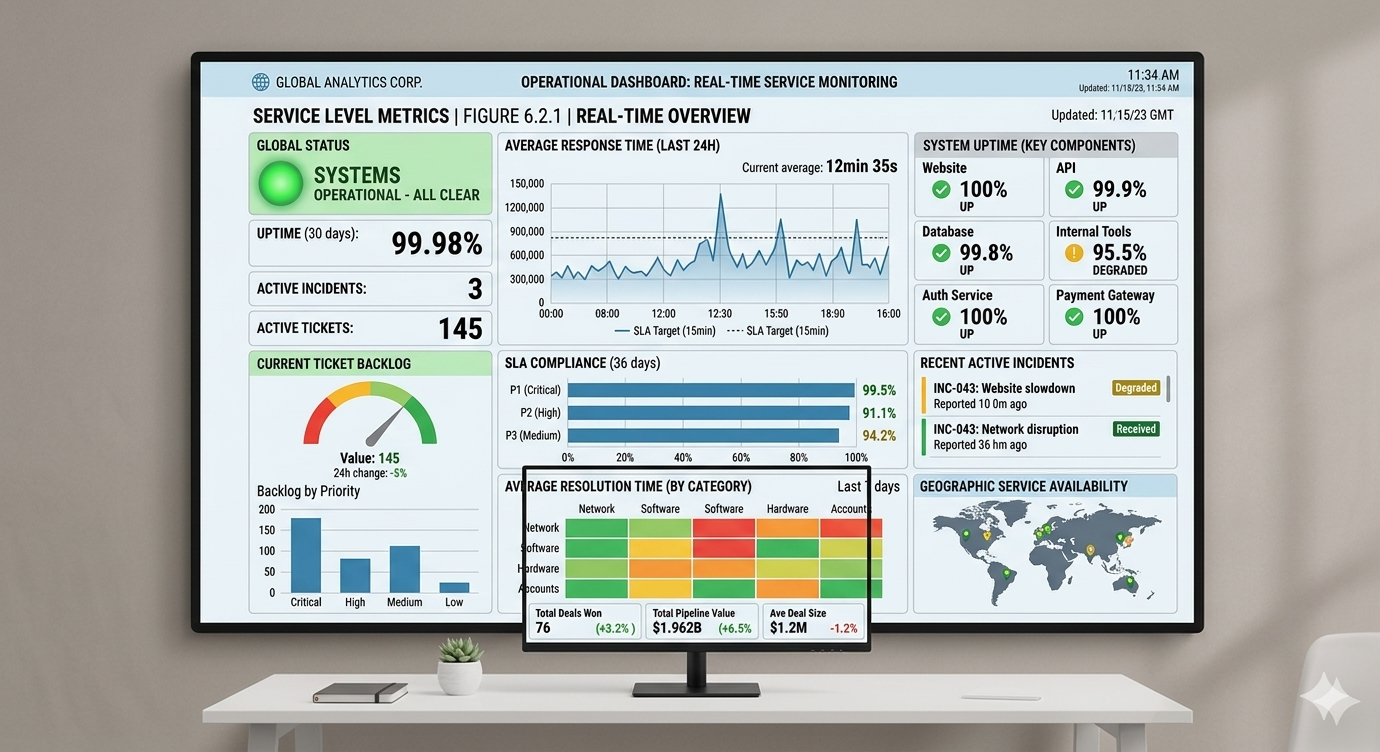
\includegraphics[width=0.85\linewidth]{slike/02/02-32.png}
    \caption{Пример оперативне контролне табле за праћење метрика нивоа услуге у реалном времену}
    \label{fig:02-17}
\end{figure}

\textbf{\textit{Тактичке контролне табле}} подржавају краткорочно и средњорочно одлучивање, типично на нивоу одељењског или функционалног менаџмента. Њихова примарна сврха је да процене трендове перформанси, упореде исходе са циљевима и ефикасније расподеле ресурсе.

За разлику од оперативних контролних табли, тактичке контролне табле ослањају се на агрегиране и сажете податке, често у распону од више недеља или месеци. Оне комбинују историјски контекст са недавним перформансама, омогућавајући корисницима да идентификују обрасце, неефикасности и настајуће ризике (Eckerson, 2011).

Кључне карактеристике тактичких контролних табли укључују:

\begin{itemize}
  \item Периодична ажурирања података (дневно, недељно)
  \item Нагласак на трендовима, поређењима и упоредним показатељима (енг. \textit{benchmark indicators})
  \item \textbf{\textit{Умерен ниво интерактивности}}
  \item Интеграцију више међусобно повезаних метрика
\end{itemize}
Типични аналитички задаци које подржавају тактичке контролне табле укључују поређење по категоријама (нпр. региони, тимови), анализу трендова током времена и анализу одступања у односу на унапред дефинисане циљеве или кључне показатеље перформанси (енг. \textbf{\textit{key performance indicators}}, KPI). Визуелизације као што су линијски графикони, груписани стубичасти графикони, топлотне мапе и мали вишеструки прикази (енг. \textbf{\textit{small multiples}}) уобичајено се користе за подршку овим задацима (Few, 2013).

\textbf{\textit{Тактичке контролне табле}} заузимају централну позицију између дескриптивне и дијагностичке аналитике, бавећи се питањима као што су „Зашто остварујемо боље или лошије резултате од очекиваних?” и „Које области захтевају корективну акцију?” (Sharda et al., 2020). Технике интеракције као што су унакрсно филтрирање и продубљивање увида (енг. \textbf{\textit{drill-down}}) посебно су важне, јер омогућавају менаџерима да пређу са сажетака високог нивоа на детаљније приказе.

\begin{figure}[h]
    \centering
    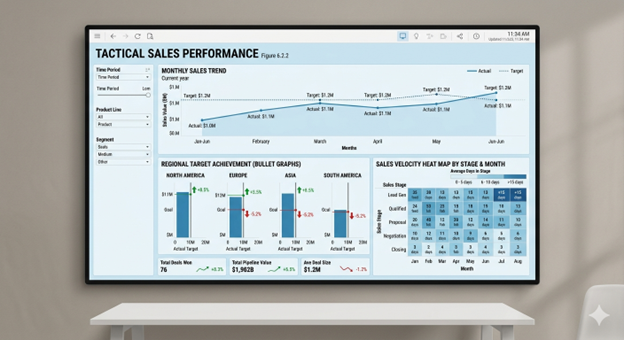
\includegraphics[width=0.85\linewidth]{slike/02/02-26.png}
    \caption{Тактичка контролна табла која приказује месечне продајне перформансе по регионима}
    \label{fig:02-18}
\end{figure}

Стратешке контролне табле намењене су подршци дугорочном одлучивању високог нивоа од стране виших руководилаца и топ менаџмента. Њихова примарна улога је да пруже интегрисан приказ организационих перформанси усклађен са стратешким циљевима.

Стратешке контролне табле типично се фокусирају на мали број критичних метрика, често изведених из оквира као што је Уравнотежени систем показатеља (енг. \textit{Balanced Scorecard}). Нагласак је на јасноћи, усклађености са циљевима и комуникацији, а не на детаљној анализи (Kaplan \& Norton, 1996; Few, 2013).

Кључне карактеристике стратешких контролних табли укључују:

\begin{itemize}
  \item Ниску учесталост освежавања података (месечно, квартално)
  \item \textbf{\textit{Висок ниво агрегације}}
  \item Снажну повезаност са стратешким циљевима и иницијативама
  \item Минималну, али пажљиво дизајнирану интерактивност
\end{itemize}
Визуелни дизајн у стратешким контролним таблама даје приоритет једноставности и доследности. Прекомерна количина детаља или сложена визуелна кодирања могу замаглити укупну поруку и смањити поверење руководилаца у контролну таблу као алат за подршку одлучивању (Few, 2013). Уобичајени визуелни облици укључују сажете KPI плочице, линије тренда и графиконе поређења високог нивоа.

\textbf{\textit{Стратешке контролне табле}} превасходно су повезане са експланаторном и прескриптивном аналитиком, бавећи се питањима као што су „Да ли смо на путу да остваримо наше стратешке циљеве?” и „Којим стратешким иницијативама треба дати приоритет?” (Sharda et al., 2020). Иако је интеракција ограничена, руководиоци могу селективно користити продубљивање увида (енг. \textbf{\textit{drill-down}}) да би проверили претпоставке или истражили узроке великих одступања.

\begin{figure}[h]
    \centering
    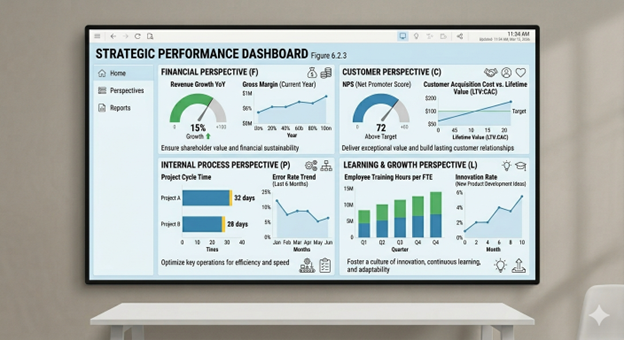
\includegraphics[width=0.85\linewidth]{slike/02/02-29.png}
    \caption{Стратешка контролна табла усклађена са оквиром Balanced Scorecard}
    \label{fig:02-19}
\end{figure}

Иако се оперативне, тактичке и стратешке контролне табле разликују по сврси и дизајну, не треба их посматрати као изоловане артефакте. У зрелим аналитичким окружењима, контролне табле на различитим нивоима логички су повезане, омогућавајући кохерентан ток од стратешких циљева ка тактичким иницијативама и оперативном извршењу (Eckerson, 2011).

\begin{table}[h]
\centering
    \caption{Поређење оперативних, тактичких и стратешких контролних табли}
    \label{tab:02-1}
\begin{adjustbox}{max width=\textwidth}
\begin{tabular}{|l|l|l|l|}
\hline
\textbf{\textit{Атрибут}} & \textbf{\textit{Оперативне}} & \textbf{\textit{Тактичке}} & \textbf{\textit{Стратешке}} \\
\hline
\textbf{\textit{Ниво одлучивања}} & Свакодневно праћење процеса; супервизори и оперативни менаџери & Краткорочно и средњорочно; одељењски/функционални менаџмент & Дугорочно; виши руководиоци и топ менаџмент \\
\hline
\textbf{\textit{Грануларност података}} & Детаљни подаци везани за конкретне активности & Агрегирани и сажети подаци (недеље/месеци) & Високо агрегиране метрике на нивоу организације \\
\hline
\textbf{\textit{Учесталост ажурирања}} & Реално или скоро реално време (секунде до минуте) & Периодично (дневно, недељно) & Ниска учесталост (месечно, квартално) \\
\hline
\textbf{\textit{Аналитички фокус}} & Дескриптивна аналитика — „Шта се дешава сада?” & Дескриптивна и дијагностичка — „Зашто резултати одступају?” & Експланаторна и прескриптивна — „Да ли смо на путу ка стратешким циљевима?” \\
\hline
\end{tabular}
\end{adjustbox}
\end{table}
Архитектура контролне табле дефинише техничку и логичку структуру која омогућава контролним таблама да поуздано трансформишу сирове податке у увиде који омогућавају деловање. Архитектура контролне табле треба се разумети не само као слој визуелизације, већ као интегрисана компонента ширег аналитичког екосистема, која обухвата изворе података, логику трансформације, семантичку апстракцију, технологије складиштења и механизме извршавања упита. Добро пројектоване архитектуре контролних табли уравнотежују перформансе, скалабилност, управљање подацима и аналитичку флексибилност, уз обезбеђивање доследности метрика и тумачења међу организационим корисницима (Chaudhuri, Dayal, \& Narasayya, 2011; Few, 2013). 

\subsection{Алати за креирање контролних табли и интерактивних извештаја}
Алати за визуелизацију и израду контролних табли се обично деле у три групе: платформе пословне интелигенције (ПИ), алате засноване на програмирању и веб-базиране оквире. Свака група има различиту намену, профил корисника и техничке могућности, па се избор доноси у односу на аналитичке захтеве, профил тима и шири аналитички екосистем.

ПИ платформе (\textit{Tableau}, \textit{Power BI}, \textit{Qlik Sense}, \textit{Looker}) покривају цео ток рада — повезивање са подацима, моделирање, израду контролних табли и дељење. Њихова основна предност је самостална аналитика: корисник без техничког предзнања истражује податке кроз „превуци и пусти” интерфејсе, док семантички слојеви и израчуната поља сакривају техничку сложеност (Few, 2013; Kimball \& Ross, 2013). Платформе су тесно повезане са складиштима података и OLAP системима, и подржавају и аналитику у меморији и непосредне упите (Inmon, 2005). Ограничења се јављају код напредног моделирања и потпуно прилагођеног дизајна (Sarikaya et al., 2019), па се ПИ платформе препоручују када су захтеви стабилни, а управљање и скалабилност важнији од потпуне флексибилности.

Алати засновани на програмирању (Matplotlib, Seaborn, ggplot2, Plotly) се користе у програмским окружењима (нпр. \textit{Python} и \textit{R}) и пружају већу слободу, репродуцибилност и аналитичку контролу. Засновани су на формалним граматикама визуелизације (Wilkinson, 2005), што омогућава прецизну контролу над сложеним вишеслојним приказима. Посебно су погодни за истраживачку анализу података и интеграцију са машинским учењем (Tukey, 1977; Wickham \& Grolemund, 2017), али захтевају програмерску стручност и разумевање перцептивних принципа (Cleveland \& McGill, 1984), због чега се претежно срећу у академским тимовима и data science улогама.

Веб-базирани оквири (D3.js, Vega-Lite, Chart.js, ECharts) проширују визуелизацију на интерактивна окружења у прегледачу. За разлику од BI платформи, они не намећу унапред дефинисане шаблоне, већ омогућавају нисконивојску контролу над графичким елементима и догађајима (Bostock et al., 2011), што их чини погодним за јавне контролне табле, уграђену аналитику и приповедање вођено подацима. Декларативни приступи као што је Vega-Lite балансирају флексибилност и апстракцију кроз JSON спецификације (Satyanarayan et al., 2017). Главно ограничење је развојна сложеност и потреба за стручношћу и у дизајну и у веб инжењерингу (Munzner, 2014).

Три групе се посматрају као комплементарне: BI платформе се користе за стандардизовано извештавање, програмски алати за напредну анализу, а веб-базирани оквири за прилагођена интерактивна решења. На постдипломском нивоу се очекује не само познавање појединачних алата, већ и разумевање како се они комбинују у ширим архитектурама подршке одлучивању.

Избор алата најчешће зависи од следећих критеријума: 

\begin{itemize}
  \item Скалабилност (података, корисника и еволуције ка архитектурама у облаку (енг. \textbf{\textit{cloud}}) и хибридним архитектурама (Knaflic, 2020).
  \item Интерактивности (Ware, 2013; Keim et al., 2008), 
  \item \textbf{\textit{Управљање и безбедност (Marr, 2016) и }}
  \item Стандардизације кроз семантичке слојеве. 
\end{itemize}
Ова четири критеријума се третирају као једнако важна и разматрају се пре, а не после, распоређивања.

\section{Складишта података}
У претходној секцији је описан кориснички слој пословне интелигенције: визуелизација, израда контролних табли, приповедање уз помоћ података и пивот табеле као свакодневни инструмент аналитичара за анализу агрегираних вредности по пословним димензијама. Све ове технике деле једну неизречену претпоставку: да је доступан чист, интегрисан, за упите оптимизован извор података и да ће захтев за годином консолидоване продаје по региону и категорији производа вратити одговор за неколико секунди, а не минута. 

\subsection{Увод у складишта података}
Складиште података је архитектонски одговор на неусклађеност радних оптерећења оперативних и аналитичких оптерећења (захтева). Оперативни системи, као што су системи за планирање ресурса предузећа (ERP), системи за управљање односима са клијентима (CRM), системи на продајном месту (енг. \textit{point-of-sale}), електронско банкарство (енг. \textit{online banking}) и слични, дизајнирани су за кратке, атомске трансакције уписа над нормализованом шемом, уз строге гаранције конзистентности (Chaudhuri \& Dayal, 1997). Аналитичка радна оптерећења имају супротан облик: дуготрајни упити само за читање, који агрегирају милионе редова кроз велики број табела и временских периода. Покретање оба оптерећења над истом базом података деградира и једно и друго: извештаји су спори, а оперативни систем трпи аналитичка скенирања током радног времена. Инмон (Inmon, 2005) је ову разлику формулисао као темељни разлог за постојање засебног, наменски изграђеног аналитичког складишта, а каснија литература, најутицајније Кимбал и Рос (Kimball \& Ross, 2013), разрадила је дизајнерске принципе који ову идеју претварају у систем који се може изградити.

\subsection{OLTP и извештавање}
Пре него што се засебно аналитичко складиште може оправдати, неопходно је прецизно утврдити шта оперативни системи раде добро и где подбацују када се поново користе за извештавање. Овај одељак разматра трансакциону базу података као дизајнерски објекат, њену нормализацију, гаранције конкурентности, обрасце приступа, а затим показује зашто свака од ових предности постаје слабост када менаџер затражи консолидован, историјски приказ са могућношћу продубљивања увида (енг. \textit{drill-down}).

\subsubsection{Трансакциони системи}
\textbf{\textit{Трансакциони системи}} (енг. \textit{online transaction processing — OLTP}) представљају оперативну основу сваке организације. Системи за планирање ресурса предузећа, системи за управљање односима са клијентима, системи на продајном месту (енг. \textit{point-of-sale}), електронско банкарство (енг. \textit{online banking}), веб-продавнице (енг. \textit{web-shop}) и апликације за људске ресурсе деле заједнички образац дизајна базе података: релациону шему у трећој нормалној форми (3NF), којој се приступа кроз кратке, атомске трансакције уписа које поштују ACID својства (Codd, 1970; Härder \& Reuter, 1983):

\begin{itemize}
  \item \textbf{\textit{Атомичност}} (енг. \textit{Atomicity}) — обезбеђује да се трансакција изврши у целости или да не остави никакав траг; делимични уписи се не дозвољавају.
  \item \textbf{\textit{Конзистентност}} (енг. \textit{Consistency}) — гарантује да се база, након успешно изведене трансакције, налази у стању које поштује све дефинисане интегритетне условности (примарни и страни кључеви, ограничења домена, окидаче).
  \item \textbf{\textit{Изолованост}} (енг. \textit{Isolation}) — значи да се истовремене трансакције извршавају као да теку секвенцијално, без међусобног утицаја на међурезултате, чиме се спречавају аномалије као што су читање непотврђених података или изгубљена ажурирања.
  \item \textbf{\textit{Трајност}} (енг. \textit{Durability}) — гарантује да резултат потврђене трансакције остаје сачуван и након отказа система, обично применом write-ahead дневника и поузданог уписа на трајни медиј (Härder \& Reuter, 1983).
\end{itemize}
ACID гаранције обезбеђују да два благајника не могу истовремено продати последњу јединицу залиха, да делимична трансакција не може оставити базу података у стању у којем је новац задужен са једног рачуна а није одобрен другом и да потврђена трансакција преживи нестанак струје. Радним оптерећењем доминирају кратке трансакције које захватају мали број редова, идентификованих примарним кључем, са захтевима за временом одзива мереним у милисекундама (Chaudhuri \& Dayal, 1997).

Да би се обезбедиле ACID особине, \textbf{\textit{нормализација података је кључни процес}} код развоја трансакционих база података.

Нормализација је поступак организације релационе шеме којим се подаци разлажу у више међусобно повезаних табела како би се елиминисала редундантност и спречиле аномалије при упису, ажурирању и брисању (Codd, 1970). Кроз сукцесивне нормалне форме (1NF, 2NF, 3NF, BCNF) се обезбеђује да сваки атрибут зависи искључиво од примарног кључа своје табеле, чиме се одржавање интегритета података своди на једно место у бази. Трећа нормална форма (3NF) се у трансакционим системима сматра практичним балансом између строге логичке доследности и прихватљивих перформанси упита, и представља уобичајени циљни ниво пројектовања OLTP шеме.

Овакав дизајн је прави одговор на проблем који оперативни систем заиста решава. Нормализација елиминише аномалије ажурирања: адреса купца се чува једном, па је њена промена ажурирање једног реда.  

Дакле нормализација података обезбеђује поштовање ACID особина, брзину уписа података као и минималну заузетост складишног простора.

\subsubsection{Цена нормализације}
Исти дизајнерски избори који OLTP системе чине одличним за бележење трансакција чине их лошим за аналитичко извештавање. Размотримо рутинско менаџерско питање: укупан приход у претходном кварталу, рашчлањен по региону и категорији производа.

Још јаснији пример је питање које менаџери заиста често постављају: „Прикажи продају по региону за последњих пет година, по кварталима, са могућношћу да се из укупног резултата спустим до категорије производа и појединачне продавнице.” У оперативном систему то питање није један природан поглед над подацима, већ скуп скупих операција над табелама чија је првобитна намена била обрада појединачних поруџбина, а не дугорочно аналитичко сажимање. Треба повезати ставке поруџбина са поруџбинама, продавницама, адресама, регионима, производима, категоријама и календаром; затим филтрирати историјски период, агрегирати на више нивоа и све то извести довољно брзо да корисник може интерактивно да настави анализу. Управо на таквим питањима постаје видљив јаз између OLTP базе и аналитичког складишта.

У нормализованој шеми, \textbf{\textit{трошак спајања табела}} (потребна меморија и време израчунавања) је висок. Одговор на претходно питање захтева спајање fact-bearing табеле ставки поруџбине са табелом купаца, табелом адреса купаца, табелом региона, табелом производа, табелом категорија производа и табелом датума. Типична оперативна шема захтева пет до десет спајања како би се саставиле колоне које су потребне једном извештају (Kimball \& Ross, 2013). Свако спајање представља додатни трошак који оптимизатор упита мора да апсорбује, а обим скенираних редова расте са кардиналношћу спајања. Извештај који враћа неколико десетина агрегираних редова може интерно пролазити кроз десетине милиона међурезултата спајања.

\textbf{\textit{Други трошак је конкуренција за ресурсе}}. Аналитички упит је само за читање, али дуготрајан; оперативно оптерећење захтева читања и уписе у исте табеле за мање од милисекунде. Покретање оба над једном базом података приморава систем на тежак компромис: закључавање на нивоу реда и одржавање индекса ради трансакционог протока, наспрам скенирања целих табела и бафера за агрегацију ради аналитичког упита, при чему свако оптерећење успорава друго. У пракси, организације које покушају да извештавају директно из OLTP система или ограничавају извештавање на пакетне прозоре ван радног времена, што искључује интерактивне контролне табле уведене у §2.1.9, или прихватају мерљиву деградацију оперативног система током радног времена.

\textbf{\textit{Трећи трошак је разумљивост}}. Нормализована шема са неколико десетина међусобно повезаних табела је непрозирна пословном кориснику. BI алати за самосталну аналитику, као што су Power BI, Tableau и Metabase, аутоматски генеришу SQL на основу корисниковог избора димензија и филтера, али је квалитет тог SQL-а онолико добар колико је добар модел кроз који се корисник креће. Када је тај модел сирова 3NF шема, корисник је приморан или да разуме путање спајања или да се ослони на мали број извештаја које је курирао IT, а ниједан од та два приступа не скалира на разноврсност ad hoc питања која уопште мотивишу програм пословне интелигенције (Kimball \& Ross, 2013). То доводи до спорог извршавања и често погрешних резултата.

\subsubsection{Шта OLTP не може}
Поред трошкова перформанси и разумљивости, постоје четири захтева која менаџери рутински постављају пред систем за извештавање, а која су структурно изван онога што OLTP база података може да понуди.

Први је \textbf{\textit{консолидовани приказ преко више система}}. Једно пословно питање, „ко су наши највреднији купци?”, типично захтева податке из ERP система (поруџбине), CRM система (интеракције), система веб-аналитике (ангажовање) и могуће спољног извора (кредитни рејтинзи). Сваки од ових система има сопствену шему, сопствене идентификаторе и сопствене дефиниције наизглед заједничких атрибута. Консолидација није проблем упита; то је проблем интеграције, којим се бави §2.2.3.3.

Други је \textbf{\textit{историјска дубина}}. OLTP систем чува текуће стање пословања: данашњу адресу купца, данашњу цену производа, данашње стање на рачуну. Када се адреса купца промени, ред се преписује и претходна адреса нестаје. Менаџер који пита како су се приходи из одређеног града развијали током три године, уопштено говорећи, не може уопште да поврати ту историју из оперативног система. Складиште података на ово одговара задржавањем сваког стања кроз које је пословање прошло, организованог по времену, што Инмон назива временском варијантношћу (Inmon, 2005), разрађеном у §2.2.3.5.

Трећи је \textbf{\textit{латенција одзива}} компатибилна са интерактивном анализом. Корисник контролне табле који чека тридесет секунди на сваку промену филтера напушта контролну таблу. Циљна латенција за аналитичке упите на савременом BI корисничком слоју (енг. \textit{front end}) је мања од секунде за кеширане агрегације и неколико секунди за ad hoc продубљивање увида (енг. \textit{drill-down}) (Chaudhuri \& Dayal, 1997). Постизање овога над нормализованом шемом са милијардама fact редова захтева архитектонске изборе, денормализацију, пре-агрегацију, колонарно складиштење, димензионо моделирање, који су некомпатибилни са OLTP дизајном.

Четврти је \textbf{\textit{продубљивање увида}} (енг. \textit{drill-down}). Корисник почиње са бројем високог нивоа, укупан приход ове године, и постепено се спушта кроз хијерархије (година → квартал → месец → дан; држава → регион → град; категорија → поткатегорија → производ) све док не стигне до нивоа детаља који објашњава варијансу. Продубљивање увида захтева да хијерархије буду експлицитно моделоване и да агрегације на сваком нивоу буду или унапред израчунате или израчунљиве у неколико секунди. OLAP коцка разматрана у §2.2.3.7 је структура података која то обезбеђује; димензионе шеме из §2.2.3.6 су оно што храни коцку.

\subsubsection{Раздвајање оперативног и аналитичког система}
Ова запажања воде ка јединственом закључку који представља консензус у овој области већ више од тридесет година: оперативна и аналитичка радна оптерећења суштински су различита и морају бити опслуживана различитим системима (Inmon, 2005; Chaudhuri \& Dayal, 1997; Kimball \& Ross, 2013). Оперативни систем задржава своју 3NF шему, ACID гаранције и перформансе уписа мерене испод милисекунде. Уз њега се гради засебан аналитички систем, складиште података, који се редовно пуни из оперативног система путем интеграционог процеса и оптимизује за радно оптерећење у којем доминирају читања, агрегације и историјска дубина. Ова два система остају лабаво повезана: складиште зависи од оперативног система као извора, али оперативни систем нема зависност од складишта, тако да аналитички упити не могу утицати на трансакциони проток.

\subsection{Складиште података}
Канонска дефиниција складишта података потиче од Вилијама Х. Инмона (William H. Inmon), који се често назива оцем складишта података: „a subject-oriented, integrated, nonvolatile, and time-variant collection of data in support of management’s decisions” (Inmon, 2005, p. 29). Сваки од ова четири придева идентификује својство које складиште мора да задовољи, а свако је негација једног својства оперативних система описаних у §2.2.2. Предметна оријентација је негација апликационе оријентације; интеграција је негација фрагментације изворних система; непромењивост је негација ажурирања на лицу места; временска варијантност је негација складиштења само текућег стања.

Из дефиниције следе три запажања. Прво, складиште података дефинисано је тиме чему служи, подршци управљачким одлукама, а не одређеном технологијом. Иста архитектонска својства могу бити имплементирана на релационој бази података, вишедимензионој бази података, колонарном механизму (енг. \textbf{\textit{engine}}) или у изворно облачном језерском складишту (енг. \textbf{\textit{cloud-native lakehouse}}). Друго, четири својства замишљена су заједно: систем који је интегрисан али волатилан, или предметно оријентисан али везан само за текуће стање, не испуњава оно што дефиниција обећава. Треће, ова својства међусобно се појачавају: непромењивост омогућава временску варијантност, а временска варијантност даје интегрисаним предметно оријентисаним подацима њихову аналитичку дубину (Inmon, 2005). §2.2.3.5 детаљно разрађује ланац зависности међу последња три својства.

Два кључна појма у складиштењу података су: 

\begin{itemize}
  \item \textbf{\textit{димензије}} (енг. \textit{dimensions}) и
  \item \textbf{\textit{мере}} (енг. \textit{measures}).
\end{itemize}
Најједноставнији начин да се они замисле јесте табеларни извештај: димензије су заглавља редова и колона, као што су регион, категорија производа и квартал, а мере су бројеви који попуњавају тело табеле, као што су приход, број продатих јединица и маржа. Димензије су описне осе дуж којих се пословање анализира и одговарају на питање „по чему” (по купцу, по производу, по датуму, по географији); мере су величине које се бележе и агрегирају дуж тих оса и одговарају на питање „колико” (број продатих јединица, приход, број запослених). Свако аналитичко питање које менаџер поставља има исти облик: једна мера, исечена по једној или више димензија и, по потреби, филтрирана.

Ови појмови се рутински мешају са табелама у којима се складиште, па је битно направити разлику између ових појмова. Табела димензије садржи описне атрибуте једне димензије, један ред по купцу у DIM\_CUSTOMER, један ред по производу у DIM\_PRODUCT, и типично је широка, денормализована и споро променљива. Табела чињеница (енг. \textit{fact table}) садржи мере које генерише један пословни процес, један ред по продајној трансакцији у FACT\_SALES, један ред по снимку стања залиха у FACT\_INVENTORY, заједно са страним кључевима ка табелама димензија које сваком мерењу дају контекст. Табеле чињеница су типично уске, дубоке и дописујуће (енг. \textit{append-only}). §2.2.3.6 разрађује обрасце шема у које се ове табеле слажу; термини се овде уводе како би дискусија о предметној оријентацији, непромењивости и временској варијантности у наредним одељцима могла слободно да их користи.

\subsubsection{Предметна оријентација}
Оперативни систем је организован око апликације која га производи. ERP систем чува фактуре и налоге за набавку, CRM систем чува контакте и кампање, систем веб-аналитике чува сесије и кликове, HR систем чува запослене и обрачун зарада. Сваки од ових система има свој модел података, своје примарне кључеве и своје конвенције; заједно они чине оно што Инмон назива пејзажом апликационих силоса (Inmon, 2005), у којем се било који појединачни пословни субјект, на пример купац, појављује као фрагментирана пројекција кроз многе системе.

Складиште података преокреће овај организациони принцип. Његове табеле су организоване око пословних субјеката о којима менаџери заиста расуђују, купаца, производа, продаје, финансија, запослених, а не око апликација које су ухватиле податке (Inmon, 2005; Kimball \& Ross, 2013). Сви подаци о купцу прикупљени су у јединствену, кохерентну репрезентацију, ослоњену на сваки изворни систем који доприноси профилу купца. Исто важи и за производе, продајни процес и сваки други субјект који је организација одлучила да третира као аналитички примаран.

Предметна оријентација има структурне последице по шему. Табеле димензија из §2.2.3.6, DIM\_CUSTOMER, DIM\_PRODUCT, DIM\_DATE, DIM\_GEOGRAPHY, предметно су оријентисане по самој конструкцији: свака је консолидован запис једног пословног субјекта, денормализован тако да су сви атрибути по којима корисник може филтрирати или груписати доступни без спајања додатних табела. Табеле чињеница које их повезују, FACT\_SALES, FACT\_INVENTORY, FACT\_PAYROLL, организоване су око пословних процеса, при чему свака табела чињеница представља мерења која произилазе из једног процеса. Ова организација чини ширу класу пословних питања непосредно одговоривом из малог скупа табела и, сходно томе, чини шему читљивом пословном кориснику који се кроз њу креће уз помоћ BI алата.

\textbf{\textit{Предметна оријентација плаћа се ценом:}} шема је денормализована, што уводи контролисану редундантност и повећава заузеће простора. У овом случају редундантност је контролисана зато што се редундантност уводи само код димензионих табела. У великој већини случајева ове табеле имају неколико редова величине мањи број случајева у односу на табелу чињеница (у којој се чувају мере тј. вредности трансакција). На пример, трговински ланац може да оствари више милиона продаја у једном дану. Са друге стране број производа може да буде мерен у стотинама (евентуално хиљадама). Имајући у виду цену данашњих складишних капацитета (нпр. хард дискова на којима се чувају подаци) релативно мали број редова са редундансом у подацима минимално подиже цену складиштења. Са друге стране остварују се велике уштеде (у времену процесирања, оптерећењу система, потребном РАМ меморијом) при аналитичком извештавању.

Унапред израчунате агрегације уводе додатни компромис: повећавају простор за складиштење и смањују грануларност у замену за брзину упита (§2.2.3.6.2). Ови компромиси се прихватају намерно зато што радно оптерећење складишта, претежно читање, претежно агрегација, латенција испод секунде, вреднује перформансе упита и читљивост шеме више од економичности складиштења. §2.2.3.6 разрађује обрасце шема кроз које се овим компромисом управља.

\subsubsection{Интеграција}
Интеграција значи да се подаци из више различитих система доведу у један усклађен облик. У пракси је проблем једноставан за опис, иако није лак за извођење: једна иста пословна ствар, на пример купац, у различитим системима често изгледа различито. Негде је записан као \texttt{customer}, негде као \texttt{client}, негде је име у једном пољу, негде у два, негде је датум у једном формату, негде у другом. Посао интеграције је да се све те разлике разреше тако да у складишту добијемо један доследан приказ.

Ове разлике се могу свести на три једноставна типа. Први су разлике у запису: исти датум може бити уписан на више начина, а иста логичка вредност као \texttt{1/0}, \texttt{Да/Не} или \texttt{True/False}. Други су разлике у структури: један систем чува пуно име у једном пољу, други у два, трећи у посебном објекту. Трећи су разлике у значењу: исти израз у два система не мора значити исто, или две различите ознаке могу означавати исту ствар. Зато интеграција није само техничко спајање табела, већ и договор шта који податак заиста значи. Најкраће речено, подаци истог значења треба да изгледају исто, а подаци различитог значења не смеју да се помешају.

Интеграција је, дакле, и процес и резултат. Процес је оно што ради ETL или ELT: преузима податке из извора, усклађује их и учитава у складиште. Резултат је оно што корисник види на крају: један усклађен приказ купаца, производа, продаје и других пословних појава. Због тога се понекад каже да складиште даје „једну верзију истине”: то не значи да је све у пословању једноставно, већ да два извештаја који користе исто складиште не би смела да дају различите бројеве за исту ствар.

\subsubsection{Непромењивост}
OLTP база података подржава четири основне операције над својим табелама: INSERT, UPDATE, DELETE, SELECT. Прве три мењају стање; последња га чита. Складиште података, насупрот томе, у нормалном раду подржава само INSERT и SELECT. Када се ред једном учита у складиште, он се не ажурира и не брише; остаје као трајни запис о томе какви су подаци били у тренутку када су забележени (Inmon, 2005). Ово својство се назива непромењивост и има две комплементарне последице.

Прва је да складиште акумулира историју. OLTP систем чува текуће стање пословања; када купац промени град, ред се преписује и претходни град се губи. То може довести до погрешних резултата упита, а последично и одлука.

Складиште, насупрот томе, задржава претходни ред и додаје нови ред који одражава промену, чија је механика предмет §2.2.3.5 о временској варијантности и §2.2.3.5.2 о споро мењајућим димензијама (енг. \textbf{\textit{slowly changing dimensions}}). Током година, ова акумулација производи историјску дубину коју аналитичка радна оптерећења захтевају. Walmart-ово складиште података, које се често наводи као пример, наводно садржи више од тридесет петабајта кроз више од две стотине милијарди редова, бележећи оперативну историју компаније на финој грануларности током животног века складишта.

Друга последица је да је складиште подложно ревизији. Пошто се ниједан ред никада не преписује и ниједан ред се никада не брише, одговор на било који историјски упит је репродуцибилан. Извештај покренут данас над подацима закључно са прошлим кварталом вратиће исте бројеве као исти тај извештај покренут прошлог квартала, зато што се основни редови нису променили. Оваква репродуцибилност структурно је немогућа у OLTP систему који преписује податке на лицу места и представља темељ на којем је изграђена улога складишта у регулаторном извештавању, финансијском затварању и подршци у парничним поступцима (Inmon et al., 2008).

Непромењивост се спроводи архитектонски, а не само као конвенција. ETL процеси који пуне складиште пишу се тако да издају само INSERT наредбе; UPDATE и DELETE над табелама чињеница складишта резервисани су за изузетне административне акције, исправљање грешке учитавања, усклађивање са законским захтевом за брисање података, и типично подлежу формалној контроли промена. Дописујући образац учитавања (енг. \textbf{\textit{append-only}}) који произилази из овог ограничења јесте оно што чини ланац зависности у §2.2.3.5 кохерентним: непромењивост омогућава временску варијантност, која се затим имплементира кроз споро мењајуће димензије (енг. \textit{slowly changing dimensions}).

\subsubsection{Временска варијантност и споро мењајуће димензије}
Временска варијантност је четврто од Инмонових својстава и оно које складишту података даје његов аналитички домет. Тамо где OLTP систем бележи како пословање изгледа сада, складиште бележи како је пословање изгледало у свакој тачки своје историје. Сваки ред у складишту је имплицитно или експлицитно означен периодом током којег је био важећи, а упити над складиштем могу питати не само „који је данас регион купца?” већ и „који је регион купца био у Q3 прошле године?”, и добити другачији, тачан одговор за сваки случај.

Временска варијантност је последица непромењивости, а не независно својство. Пошто складиште никада не преписује ред, свако стање кроз које је пословање прошло остаје у табели; оно што временска варијантност додаје јесте дисциплина означавања сваког реда његовом временском ваљаношћу тако да се историјска стања могу упитивати на принципијелан начин. Ланац, непромењивост омогућава временску варијантност, која се операционализује кроз димензиони третман промене, представља образац дизајна наредног потодељка.

Однос међу последња три Инмонова својства је узрочан. Непромењивост је архитектонско ограничење: складиште дописује уместо да ажурира. Временска варијантност је последица: пошто се ништа не преписује, табела акумулира временски запис сваке промене. Споро мењајуће димензије (енг. \textit{slowly changing dimensions}, SCDs) јесу имплементација: скуп стратегија помоћу којих складиште одлучује како, тачно, да забележи промену у атрибуту димензије (Kimball \& Ross, 2013).

Ознака “slowly changing” одражава емпиријско запажање да се атрибути ентитета димензија, адреса купца, категорија производа, одељење запосленог, мењају ретко у поређењу са брзином којом се додају fact редови. Они се, ипак, мењају, а складиште мора одлучити шта да ради када до промене дође. Та одлука је значајна зато што се иста димензија референцира из историјских fact редова, а избор стратегије одређује да ли ће се ти историјски редови читати у односу на текуће стање димензије или у односу на стање димензије у тренутку када се fact догодио.

Кимбал и Рос (Kimball \& Ross, 2013) каталогизују четири канонске стратегије за руковање променом димензије, нумерисане од 0 до 3. Свака представља различит избор о томе шта се чува, а шта губи, и прави избор за било који атрибут зависи од аналитичких питања која складиште треба да подржи.

\begin{figure}[h]
    \centering
    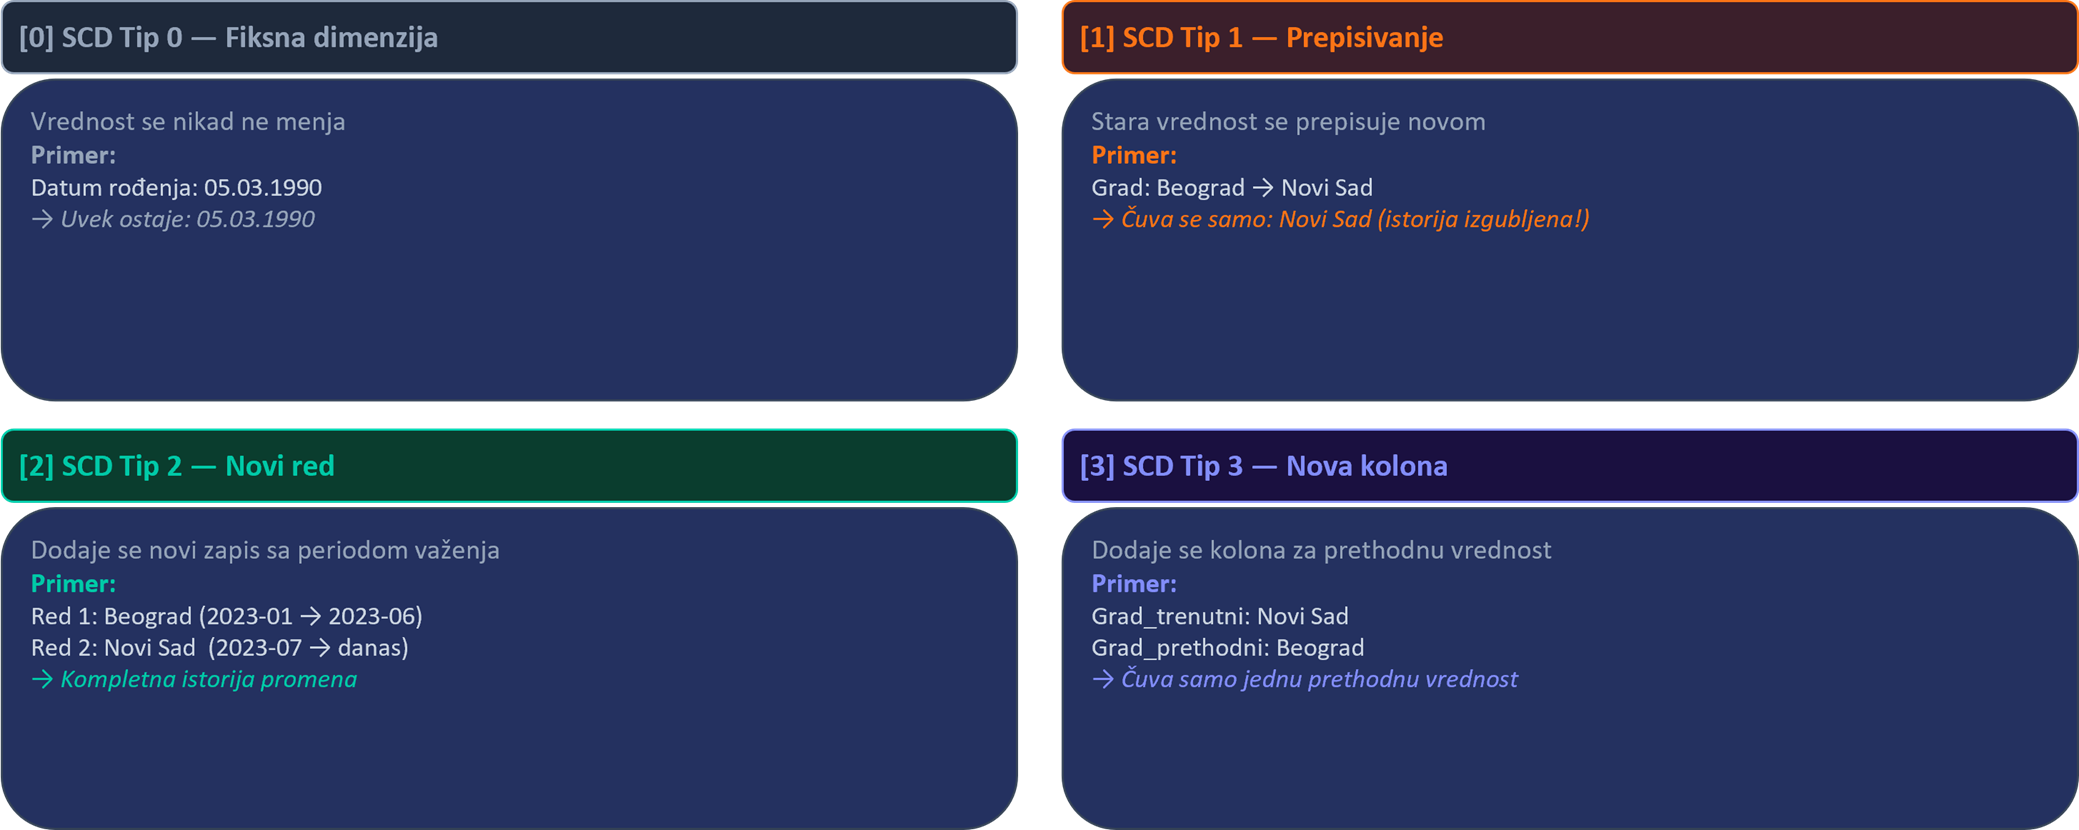
\includegraphics[width=0.85\linewidth]{slike/02/02-25.png}
    \caption{Споро мењајуће димензије (енг. slowly changing dimensions): типови 0–3, четири стратегије за руковање променом у атрибуту димензије}
    \label{fig:02-20}
\end{figure}

\textbf{\textit{SCD Type 0 — фиксна димензија.}} Атрибут се третира као непроменљив: када се једном забележи, више се никада не мења. Type 0 је прави избор за атрибуте који се заиста не могу мењати, датум рођења купца, датум прве производње производа, а погрешан избор за све остало, јер његова примена на променљив атрибут једноставно значи да складиште тихо губи кореспонденцију са стварношћу.

\textbf{\textit{SCD Type 1 — преписивање.}} Када дође до промене, постојећи ред се ажурира на лицу места; претходна вредност се губи. Type 1 је исправан само када историја није важна и када је најновија вредност једина вредност која ће складишту икада бити потребна. То је најједноставнија стратегија за имплементацију и најопаснија за примену као подразумевана, она унутар самог складишта поново уводи управо ону волатилност коју архитектура постоји да спречи. Радни пример у наставку овог одељка показује како примена Type 1 на атрибут који се користи за груписање тихо корумпира сваки историјски извештај.

\textbf{\textit{SCD Type 2 — нови ред.}} Када дође до промене, постојећи ред се затвара постављањем крајњег датума, а убацује се нови ред са новом вредношћу атрибута, отвореним крајњим датумом и новим сурогат кључем. Type 2 чува потпуну историју димензије: сваки ред носи период важења (datum\_od, datum\_do), и сваки историјски fact спојен са својом верзијом димензије преузима вредност атрибута онакву каква је била када је fact забележен. Type 2 је доминантна стратегија у пракси и стандардни избор за сваки атрибут димензије који се користи у историјској анализи (Kimball \& Ross, 2013).

\textbf{\textit{SCD Type 3 — нова колона.}} Када дође до промене, постојећи ред се ажурира на лицу места, али нова колона бележи претходну вредност. Type 3 чува тачно једно историјско стање, најновију промену, и прикладан је за атрибуте код којих корисници желе да упореде „тренутно” са „претходним”, али им није потребна пуна историја, на пример реорганизација продајне територије, где колона previous-territory подржава year-over-year извештаје током транзиције.

SCD Type 2 захтева структуру кључева која разликује верзије истог пословног ентитета, и управо ту сурогат кључ зарађује своје централно место у димензионом моделирању (Kimball \& Ross, 2013). Природни кључ је идентификатор који користе пословање и изворни системи, ID купца, SKU производа, национални идентификациони број. Природни кључ идентификује ентитет, али не разликује његове верзије: купац 1001 има један природни кључ без обзира на то да ли складиште садржи њен ред за Београд из 2021. или ред за Нови Сад из 2024.

Сурогат кључ је вештачки цео број који генерише само складиште, типично помоћу IDENTITY колоне или механизма секвенце (енг. \textit{sequence}), и који јединствено идентификује један ред у табели димензије. Свака верзија ентитета добија сопствени сурогат кључ: ред купца 1001 за Београд из 2021. може имати сурогат кључ 501, а ред за Нови Сад из 2024. сурогат кључ 502. Табеле чињеница складишта затим референцирају димензије преко сурогатног кључа, никада преко природног кључа. Резултат је да ред табеле чињеница забележен 2022. носи сурогатни кључ 501 у колони customer\_sk и спаја се са верзијом купца 1001 за Београд, што је било стварно стање купца у то време. Ред табеле чињеница забележен 2024. носи сурогатни кључ 502 и спаја се са верзијом за Нови Сад. Сваки такав ред чува се у односу на стање димензије под којим се заиста догодио.

Сурогат кључеви су независни од кључева изворних система и преживљавају њихове промене; омогућавају чланове “unknown” или “not applicable”, типично са резервисаним кључевима као што су 0 или -1, без загађивања простора природних кључева; и уједначено су целобројног типа кроз све димензије, што поједностављује спајања и индексирање. Ове секундарне предности су разлог што се сурогат кључеви препоручују чак и за димензије које нису подложне Type 2 верзионисању (Kimball \& Ross, 2013).

Претпоставимо да складиште примењује SCD Type 1 на атрибут град. Када дође до промене у јануару 2024, поље city у реду купца бива преписано са “Beograd” на “Novi Sad”; претходна вредност нестаје. Извештај о приходу по граду, написан као спајање из FACT\_SALES кроз DIM\_CUSTOMER по природном кључу и груписан по граду, сада приписује свих 580.000 RSD купчевих животних куповина Новом Саду, укључујући и 500.000 RSD који су заправо купљени док је купац живео у Београду. Ред за Београд у извештају показује нулу. Број је погрешан, и што је још горе, сам извештај је структурно неспособан да буде исправан: подаци потребни да би се историјска продаја доделила исправном граду су преписани и више нису у складишту.

\begin{figure}[h]
    \centering
    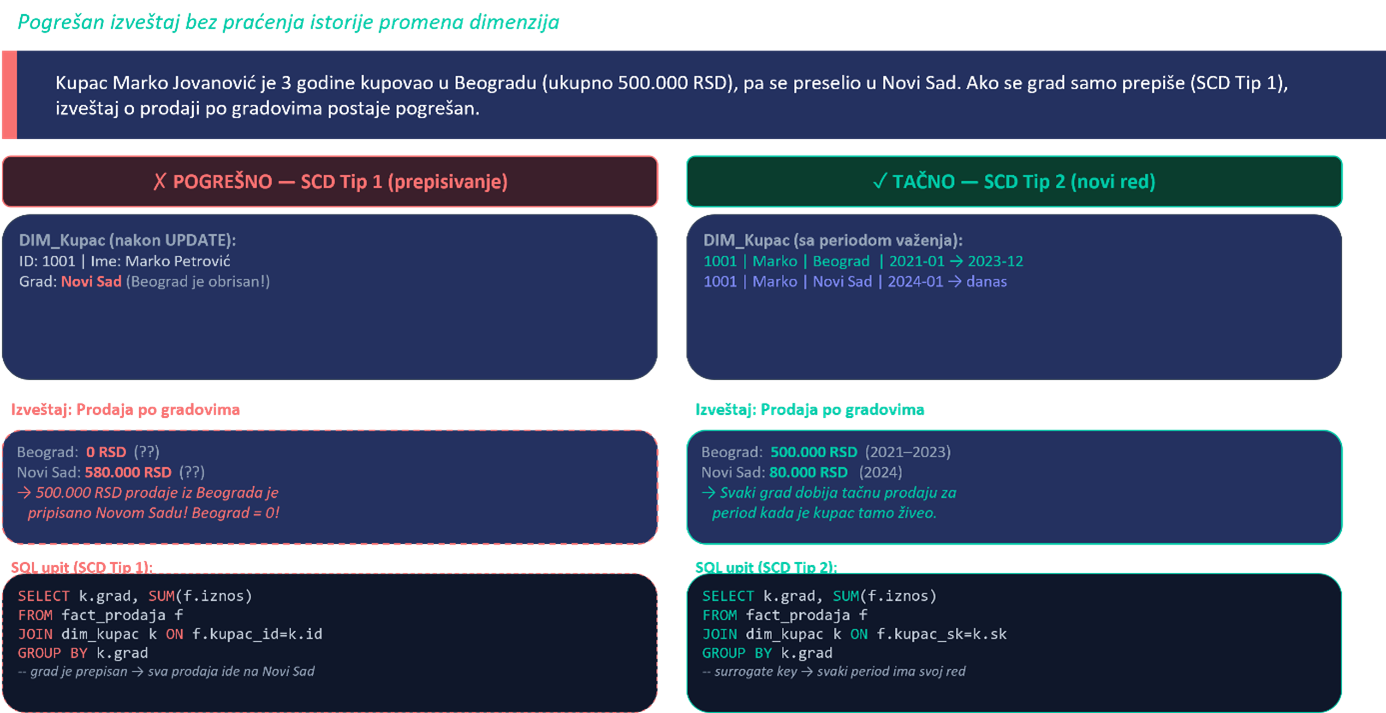
\includegraphics[width=0.85\linewidth]{slike/02/02-06.png}
    \caption{Промена града купца: Type 1 (лево) погрешно приписује историјски приход из Београда Новом Саду; Type 2 (десно) чува период важења и враћа исправан приход по граду}
    \label{fig:02-21}
\end{figure}

Претпоставимо да складиште примењује SCD Type 2. Постојећи ред димензије купца затвара се крајњим датумом 31. децембар 2023. и сурогат кључем 501; убацује се нови ред са сурогат кључем 502, новим градом Нови Сад, почетним датумом 1. јануар 2024. и отвореним крајњим датумом. Fact редови забележени између 2021. и 2023. носе customer\_sk = 501 и спајају се са верзијом за Београд; fact редови забележени од 2024. па надаље носе customer\_sk = 502 и спајају се са верзијом за Нови Сад. Исти упит прихода по граду, сада написан као спајање по сурогат кључу, враћа 500.000 RSD за Београд и 80.000 RSD за Нови Сад. Сваки град добија приход који је заиста остварен док је купац тамо живео.

Пример је мали, али поука коју даје је општа: примена SCD Type 1 на атрибут који се користи за груписање тихо корумпира сваки историјски извештај који по њему групише, а корупција се не може открити из самог извештаја, бројеви се сабирају у исправан укупан збир, само су погрешно распоређени по групама. Избор SCD стратегије стога није технички детаљ већ суштинска одлука моделирања и мора бити донет намерно за сваки атрибут сваке димензије коју складиште излаже за груписање.

\subsubsection{Димензионо моделовање}
Четири својства из §§2.2.3.1–2.2.3.5 одређују шта складиште података мора бити; она не одређују како су његове табеле распоређене. Зато, ова секција следи препоруке Кимбала и Роса (Kimball \& Ross, 2013) и усваја димензионо моделирање као радни дизајн шеме. Димензионо моделирање организује складиште у две врсте табела, табеле чињеница и табеле димензија, и прописује мали број канонских образаца шема који их комбинују. Ова секција уводи те две врсте табела, разрађује четири канонска обрасца, једнотабеларни, звездасти, пахуљасти и галаксијски, и третира грануларност као дизајнерску одлуку од које зависи остатак шеме.

\paragraph{Чињенице и димензије}
Табела чињеница бележи мерења која произилазе из пословног процеса: продату количину и остварени приход за сваку ставку сваке поруџбине, ниво залиха за сваки производ у сваком складишту сваког дана, исплаћену зараду сваком запосленом у сваком платном периоду и оцену студента на испиту. Редови табеле чињеница су догађаји или стања; колоне су нумеричке мере повезане са сваким од њих (Kimball \& Ross, 2013). 

Мере у табелама чињеница типично су \textbf{\textit{адитивне}}: количине и износи природно се сабирају преко било које комбинације димензија. Неке мере су \textbf{\textit{полуадитивне}}, ниво залиха не може се сабирати преко дана али може преко складишта, а неке су \textbf{\textit{неадитивне}}, као што су јединична цена или просечан однос. У већини случајева мерења морају бити представљена као нумеричке вредности. Међутим, постоје случајеви када се мерења могу израчунати на основу категоријалних вредности. На пример: број, или различит број, купаца. Овде се могу користити категоријалне вредности, нпр. CustomerID, али је агрегатна функција count, односно count distinct. И други примери су уобичајени: број различитих производа купљених по поруџбини, број продавница које су имале артикал на стању у одређеној недељи, број јединствених посетилаца веб-странице или број запослених који су завршили курс обуке. Агрегатне функције које се примењују над табелама чињеница стога су разноврсне. 

Нумеричке мере се најчешће сабирају (SUM) или усредњавају (AVG); полуадитивне мере се типично сабирају преко неких димензија, а усредњавају или узимају у одређеном тренутку преко других, ниво залиха сабран преко складишта али усредњен преко дана, или прочитан на крају месеца. Поред SUM, AVG, COUNT и COUNT DISTINCT, уобичајене функције укључују MIN и MAX, највећи износ фактуре у кварталу, најранији датум поруџбине за купца, MEDIAN и процентилне агрегате (енг. \textbf{\textit{percentile aggregates}}), медијалну вредност поруџбине, 95. перцентил времена испоруке, STDDEV и VAR, волатилност дневне продаје, и односне мере (енг. \textbf{\textit{ratio measures}}) изведене из два основна збира, као што су бруто маржа, приход минус трошак подељен приходом, и стопа конверзије, број поруџбина подељен бројем сесија. Избор агрегатне функције је својство саме мере, а не упита, и мора бити декларисан у семантичком слоју тако да BI алати доследно агрегирају кроз извештаје.

Табела димензије бележи контексте, односно димензије у односу на које се табеле чињеница анализирају: купца који је извршио поруџбину, производ који је продат, датум када је продаја извршена и географију у којој купац живи. Редови табеле димензије су ентитети или чланови; колоне су атрибути тих ентитета по којима корисник жели да филтрира, групише или врши продубљивање увида (енг. \textit{drill-down}). Димензије су типично широке, имају много атрибута и плитке су, односно садрже релативно мало редова у поређењу са табелама чињеница, а денормализоване су тако да се регион, држава и континент појављују као колоне у DIM\_GEOGRAPHY, а не као засебне нормализоване табеле. Тако је упиту потребно само једно спајање са табелом чињеница да би преузео било који атрибут контекста.

Табеле чињеница и табеле димензија повезане су страним кључевима на сурогат кључеве: сваки ред у FACT\_SALES носи customer\_sk, product\_sk, date\_sk и geography\_sk, а сваки од њих спаја се са одговарајућом табелом димензије по њеном сурогат кључу. Дисциплина ограничавања страних кључева табеле чињеница на сурогат кључеве и денормализације сваке димензије у једну широку табелу јесте оно што димензионим шемама даје њихове аналитичке перформансе и читљивост за BI алате.

\paragraph{Грануларност}
Пре него што се дефинишу димензије и табеле чињеница, дизајнер мора да одговори на питање: шта представља један ред табеле чињеница? Одговор на ово питање дефинише грануларност (енг. \textit{grain}), односно ниво детаља података, а Кимбал и Рос (Kimball \& Ross, 2013) стављају је у средиште процеса дизајна: најпре се декларише грануларност, затим се идентификују димензије које су с њом конзистентне, па тек онда мере које су на том нивоу грануларности адитивне.

Грануларност исказана у једној реченици, „један ред по ставци сваке фактуре”, „један ред по пакету скенираном на сваком кораку сваке пошиљке”, „један ред по минуту сваког позива”, дисциплинује сваки наредни дизајнерски избор.

Избор грануларности је компромис. Најфинија (највиши ниво) могућа грануларност, један ред по атомском пословном догађају, чува сваки детаљ, али производи највеће табеле чињеница и најспорије упите. Грубља (нижи ниво) грануларност, дневни сажеци уместо појединачних трансакција, месечни сажеци уместо дневних, смањује број редова и убрзава упите по цену детаља. Пример на наредној слици репродукује пример детаљних записа о позивима (енг. \textbf{\textit{call-detail records}}) из изворне презентације: телекомуникациони оператор може чувати појединачне записе о позивима (Слика~\ref{fig:02-22}) (200 редова, 4.000 бајтова по кориснику месечно) на једној крајности и један месечни сажет ред (један ред, 200 бајтова по кориснику месечно) на другој. Сажетак је двадесет пута ефикаснији у простору и бржи за упите, али не може одговорити на питања о појединачним позивима.

\begin{figure}[h]
    \centering
    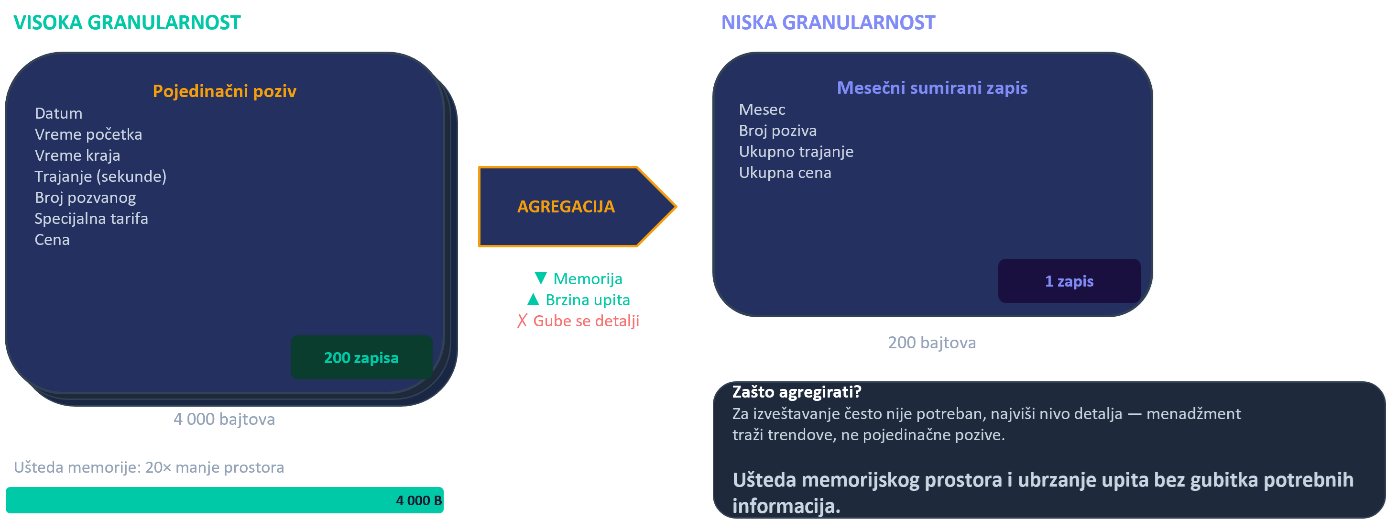
\includegraphics[width=0.85\linewidth]{slike/02/02-12.png}
    \caption{Компромис грануларности: атомски записи детаља позива (енг. call-detail records) насупрот месечним сажетим редовима}
    \label{fig:02-22}
\end{figure}

У пракси, складишта чувају најфинији доступан ниво грануларности и ослањају се на агрегацију како би по потреби произвела грубље приказе (Kimball \& Ross, 2013). Унапред израчунате агрегатне табеле, дневни сажетак изведен из табеле чињеница на нивоу трансакције, месечни сажетак изведен из дневног, убрзавају најчешће упите, док атомска табела чињеница остаје доступна за непредвиђена питања. OLAP коцка из §2.2.3.7 представља генерализацију ове идеје: она унапред израчунава агрегације преко сваке релевантне комбинације нивоа димензија.

\paragraph{Схеме складишта података}
Четири схеме складишта података димензионим моделирањем. Они се разликују по томе како мењају редундантност за перформансе упита и колико пословних процеса могу да обухвате.

\textbf{\textit{Једнотабеларна шема}} (енг. \textit{flat schema}). Сви атрибути, чињенице и свака контекстуална колона чувају се у једној денормализованој табели. Упити не захтевају спајања и враћају веома брзе резултате, али је табела веома редундантна, регион купца се понавља у сваком продајном реду, трошак складиштења је висок, а свако ажурирање контекстуалног атрибута захтева дотицање сваког реда чињенице. Једнотабеларна шема погодна је за мале, једноставне скупове података и за неке имплементације колонарних складишта где се редундантност добро компресује; она не скалира на складишта на нивоу предузећа.

\begin{figure}[h]
    \centering
    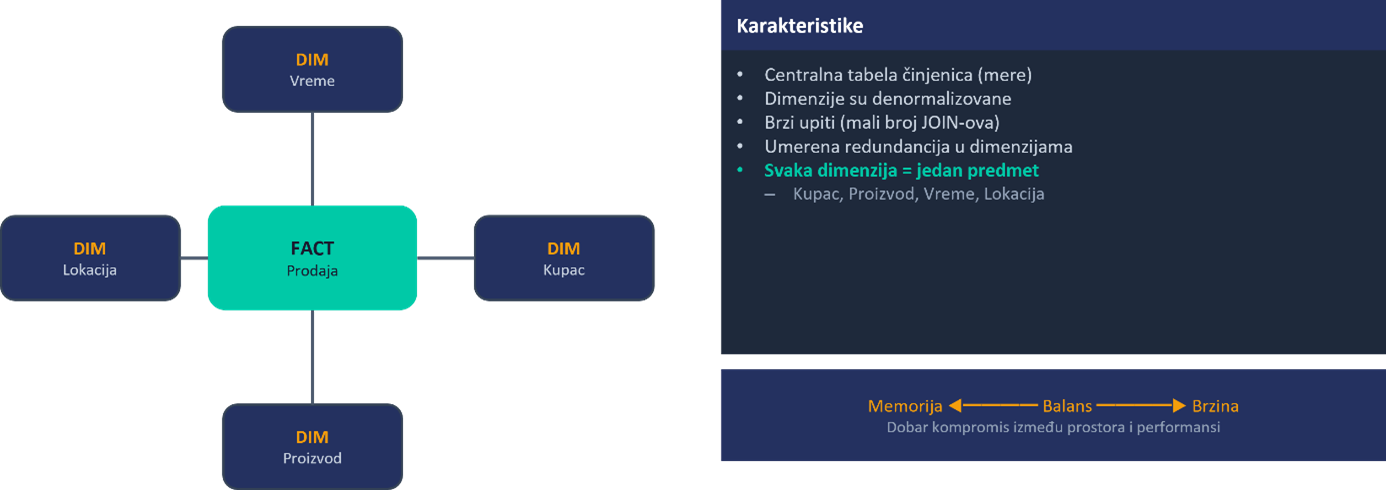
\includegraphics[width=0.85\linewidth]{slike/02/02-10.png}
    \caption{Звездаста шема (енг. star schema): централна fact табела окружена денормализованим димензијама}
    \label{fig:02-23}
\end{figure}

Звездаста шема (енг. star schema). Табела чињеница је повезана са денормализованим димензионим табелама на једном нивоу спајања, при чему свака димензија има један примарни кључ који се као страни кључ налази у табели чињеница. Иако су димензионе табеле денормализоване, шема заузима драстично мање складишног простора него једнотабеларна — контекстуални атрибути се не понављају у сваком реду чињенице, већ се спајају по потреби. Извештавање је нешто спорије од једнотабеларне шеме због неопходних спајања, али је и даље брзо: модел остаје једноставан за разумевање и оптимизацију, па је звездаста шема најчешћи избор у складиштима података на нивоу предузећа (Kimball \& Ross, 2013).

\begin{figure}[h]
    \centering
    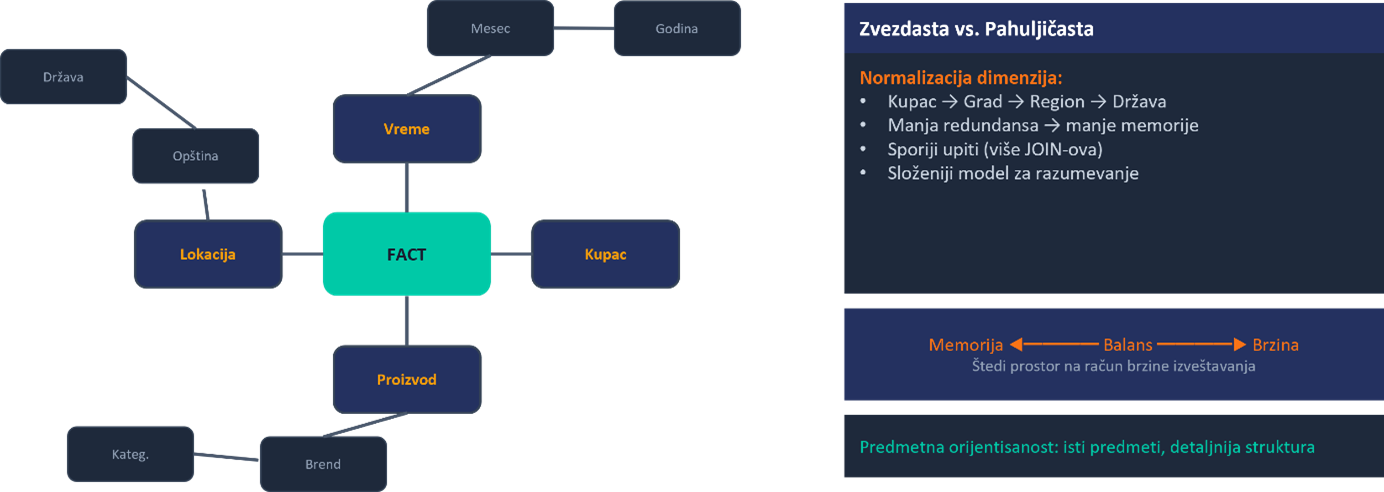
\includegraphics[width=0.85\linewidth]{slike/02/02-14.png}
    \caption{Пахуљаста шема (енг. snowflake schema): димензије нормализоване у поддимензије, чиме се смањује редундантност по цену додатних спајања}
    \label{fig:02-24}
\end{figure}

Пахуљаста шема (енг. snowflake schema). Димензионе табеле (једна или више њих) су нормализоване, обично до 3NF, тако да се хијерархијски атрибути (нпр. град → регион → држава, производ → подкатегорија → категорија) разлажу у засебне поддимензионе табеле повезане преко страних кључева. Редундантност се додатно смањује и описни атрибути се одржавају на једном месту, али упити захтевају више спајања, па је извештавање спорије од звездасте шеме. Пахуљаста шема се користи када су димензионе хијерархије стабилне, када је заузеће складишног простора критично или када се захтева строг интегритет описних атрибута.

\begin{figure}[h]
    \centering
    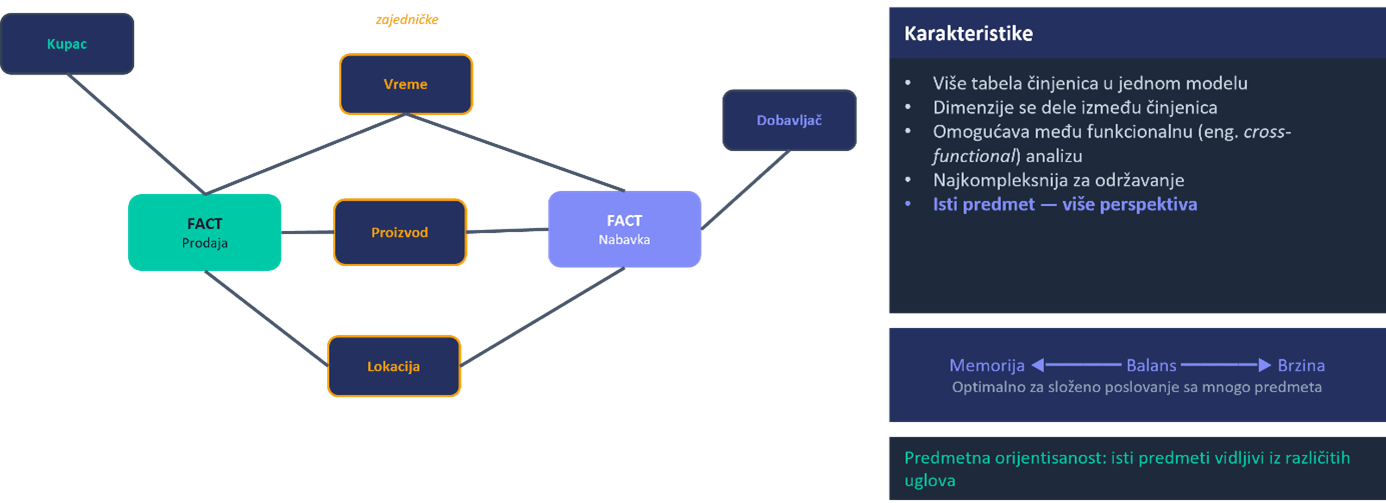
\includegraphics[width=0.85\linewidth]{slike/02/02-19.png}
    \caption{Галаксијска шема (енг. galaxy schema, fact constellation): више fact табела које деле заједнички скуп усаглашених димензија (енг. conformed dimensions)}
    \label{fig:02-25}
\end{figure}

Галаксијска шема (енг. galaxy schema, fact constellation). Више табела чињеница из различитих пословних процеса дели заједнички скуп усаглашених димензија (енг. conformed dimensions), па се иста димензиона табела (нпр. време, купац, производ) користи за више независних мерења. Шема омогућава унакрсну анализу процеса — на пример, поређење продаје и рекламација по истим димензијама — али је сложенија за пројектовање и одржавање јер захтева доследну дефиницију усаглашених димензија на нивоу целог складишта. Користи се у зрелим складиштима података на нивоу предузећа која покривају више међусобно повезаних пословних процеса (Kimball \& Ross, 2013).

\subsubsection{OLAP коцке и пивот табеле}
Димензионе шеме чине аналитичке упите брзим; OLAP коцке их чине тренутним. Ова секција уводи вишедимензиону структуру која је постала стандардни аналитички слој складишта података, разликује три архитектуре складиштења путем којих се она имплементира и затвара круг са пивот табелом, формално, клијентом коцке, која проширује интерактивне аналитичке технике разрађене у §2.1.8. 

\paragraph{OLAP коцка}
Термин аналитичка обрада на мрежи (енг. \textit{online analytical processing}, OLAP) увели су Код, Код и Сали (Codd, Codd, \& Salley, 1993) како би разликовали аналитичко радно оптерећење, вишедимензионо, агрегирајуће и истраживачко, од трансакционог радног оптерећења (OLTP) оперативних система. OLAP коцка је структура података која подржава ово радно оптерећење (Слика~\ref{fig:02-26}): вишедимензиони низ у којем свака димензија одговара једној аналитичкој оси (време, производ, географија, купац), а свака ћелија на пресеку чланова димензија садржи агрегирану меру (збир прихода, број поруџбина, просечну маржу). Код, Код и Сали (Codd, Codd, \& Salley, 1993) и Чаудхури и Дајал (Chaudhuri \& Dayal, 1997) пружају темељне описе; Кимбал и Рос (Kimball \& Ross, 2013) третирају коцку као природну, за читање оптимизовану пројекцију звездасте или галаксијске шеме.

Коцка се гради из табеле чињеница унапред израчунавањем сваке агрегације која би могла бити од интереса дуж димензија коцке: укупан приход по години, по кварталу, по месецу и по дану; по држави, по региону и по граду; и по свакој комбинацији ових. Агрегације се чувају у индексираној структури која подржава проналажење по координатама димензија. Упит који тражи приход по граду за 2024. не скенира табелу чињеница и не израчунава SUM и GROUP BY у реалном времену; он врши индексирано проналажење унапред израчунате ћелије на координати (Time = 2024, Geography = сваки град) и одмах враћа одговор. Тамо где би SQL упит над табелом чињеница од милиона редова могао трајати од пет до тридесет секунди, коцка враћа резултат за мање од секунде (Chaudhuri \& Dayal, 1997).

Најједноставнији начин да се коцка интуитивно разуме јесте пример са три димензије: време × производ × регион. Замислимо да једна ћелија коцке садржи укупан приход за комбинацију „Q1 2025, млечни производи, Београд”. Ако аналитичар фиксира време на 2025. годину и посматра само производе и регионе, извео је пресек коцке (енг. \textbf{\textit{slice}}). Ако затим ограничи и време на први квартал и регион на Србију север, добија ужи подскуп (енг. \textbf{\textit{dice}}). Ако из приказа „2025” пређе на „Q1, Q2, Q3, Q4”, изводи продубљивање увида (енг. \textbf{\textit{drill-down}}) дуж временске хијерархије; ако се из месеци врати на године, ради сажимање на виши ниво (енг. \textbf{\textit{roll-up}}). Управо ове операције стоје иза утиска да се пивот табела или контролна табла „одмах” преобликује када корисник промени ниво посматрања.

\begin{figure}[h]
    \centering
    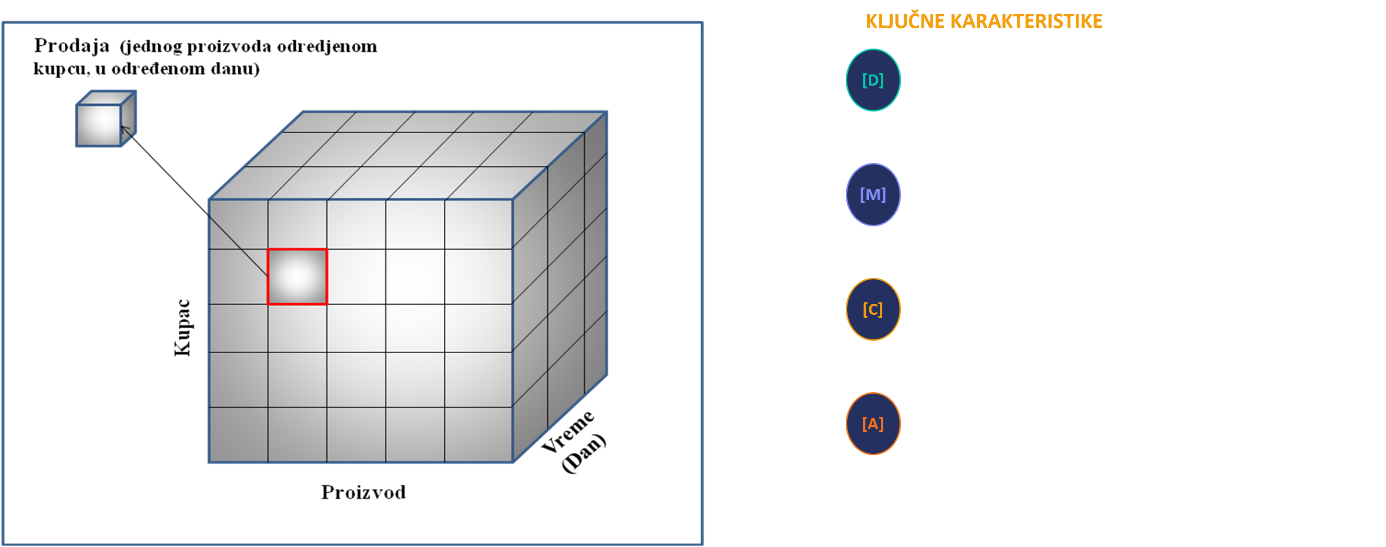
\includegraphics[width=0.85\linewidth]{slike/02/02-08.png}
    \caption{OLAP коцка: вишедимензиона структура у којој свака ћелија садржи унапред израчунату агрегирану меру}
    \label{fig:02-26}
\end{figure}

Стандардне аналитичке операције над коцком су:

\begin{itemize}
  \item \textbf{\textit{пресек}} (енг. \textit{slice}; фиксирање једне димензије на вредност, нпр. Time = 2024),
  \item \textbf{\textit{подскуп}} (енг. \textit{dice}; фиксирање више димензија, нпр. Time = 2024 и Region = Vojvodina),
  \item \textbf{\textit{продубљивање увида}} (енг. \textit{drill-down}; спуштање низ хијерархију, нпр. са године на квартал па на месец),
  \item \textbf{\textit{сажимање на виши ниво}} (енг. \textit{roll-up}; пењање уз хијерархију), и
  \item \textbf{\textit{ротација}} (енг. \textit{pivot}; излагање различитог пара димензија у унакрсној табелацији).
\end{itemize}
Свака од ових операција директно одговара радњи коју корисник предузима на контролној табли или пивот табели, због чега се коцка и пивот табела тако природно уклапају.

\paragraph{Пивот табела као OLAP клијент}
Пивот табела, аналитичарев инструмент за унакрсно табелирање мера кроз две или више димензија, допуњује интерактивне технике из §2.1.8. Када је коцка успостављена, пивот табела добија своју формалну улогу: она је клијент OLAP коцке. Корисников избор редова, колона, филтера и мера спецификује упит у координатном простору коцке, коцка враћа претходно агрегиране ћелије које одговарају том упиту, а пивот табела их приказује као унакрсну табелацију. Када корисник превуче нову димензију у област редова, пивот табела издаје нови упит коцки на новом нивоу грануларности; када корисник прошири хијерархију, пивот табела издаје упит за продубљивање увида (енг. \textbf{\textit{drill-down}}). Интеракција коју аналитичар доживљава као тренутну, испод површине је низ индексираних претрага коцке.

Овај однос има практичне последице. Пивот табела која ради директно над радним листом изворних података ограничена је лимитима радног листа — Excel-ово ограничење редова је приближно милион по листу — и меморијским агрегирајућим механизмом табеларног калкулатора. Насупрот томе, пивот табела повезана са OLAP коцком ради над претходно агрегираним ћелијама које се чувају на серверу и ограничена је величином коцке, а не величином табеларног листа. Excel пивот табеле могу бити подешене да користе Analysis Services коцке као извор података; кориснички интерфејс је познати табеларни калкулатор, али су упити MDX (Multidimensional Expressions, стандардни језик упита за OLAP коцке), а не SQL, и обим података се протеже до милијарди редова чињеница.

Читалац стога може задржати интуицију да је пивот табела алат за сечење, груписање и филтрирање, тесно повезан са интерактивним техникама из §2.1.8, и томе додати архитектонску слику коју је овај одељак развио. Пивот табела припада корисничком слоју (енг. \textbf{\textit{front end}}); OLAP коцка је аналитички слој оптимизован за читање који стоји иза ње; коцка се гради из звездасте или галаксијске шеме (енг. \textit{star} или \textit{galaxy schema}); шема се пуни из изворних система ETL процесом; и целокупан овај распоред постоји зато што OLTP системи описани у §2.2.2 не могу, сами по себи, да одговоре на питања која менаџери постављају својим подацима.

\paragraph{MOLAP, ROLAP и HOLAP}
Три имплементационе архитектуре доминирају, а разликују се по томе где се подаци коцке чувају и како им се приступа (Chaudhuri \& Dayal, 1997).

Multidimensional OLAP (MOLAP) смешта коцку у наменски изграђену вишедимензионалну базу података која материјализује агрегације у компресованој, индексираној структури. Упити су изузетно брзи зато што се одговори читају директно из индексираних ћелија; цена су велики иницијални захтеви за складиштењем и дуготрајан процес изградње коцке када се основне чињенице промене. Microsoft Analysis Services и Oracle Essbase су репрезентативни MOLAP механизми.

Relational OLAP (ROLAP) чува коцку као скуп табела у релационој бази података — типично у истом складишту које садржи основне чињенице — и одговара на упите над коцком тако што их преводи у SQL са одговарајућим агрегацијама. Складиштење је ефикасније јер агрегације нису у потпуности унапред материјализоване, а архитектура се природно скалира на веома велике табеле чињеница; цена су спорији појединачни упити зато што SQL агрегација мора да се изврши у тренутку упита, чак и када јој помажу aggregate tables и column-store индекси. SAP BW и MicroStrategy су репрезентативне ROLAP платформе.

Hybrid OLAP (HOLAP) комбинује ова два приступа: агрегиране вредности се чувају у вишедимензионалној структури ради брзих упита сажимања на виши ниво (енг. \textbf{\textit{roll-up}}), док основни детаљни редови остају у релационом складишту ради продубљивања увида (енг. \textbf{\textit{drill-down}}) до атомског нивоа грануларности. HOLAP је подразумевани режим већине савремених OLAP механизама јер обухвата већину MOLAP перформанси упита уз већину ROLAP економичности складиштења. Компромиси између ове три архитектуре могу се сажети овако: брзина упита иде редом MOLAP > HOLAP > ROLAP, док и трошак складиштења следи исти редослед. Избор зависи од величине табела чињеница, захтева за кашњењем BI корисничког слоја (енг. \textit{front end}) и расположивог буџета за рачунарске ресурсе и складиштење.

\begin{figure}[h]
    \centering
    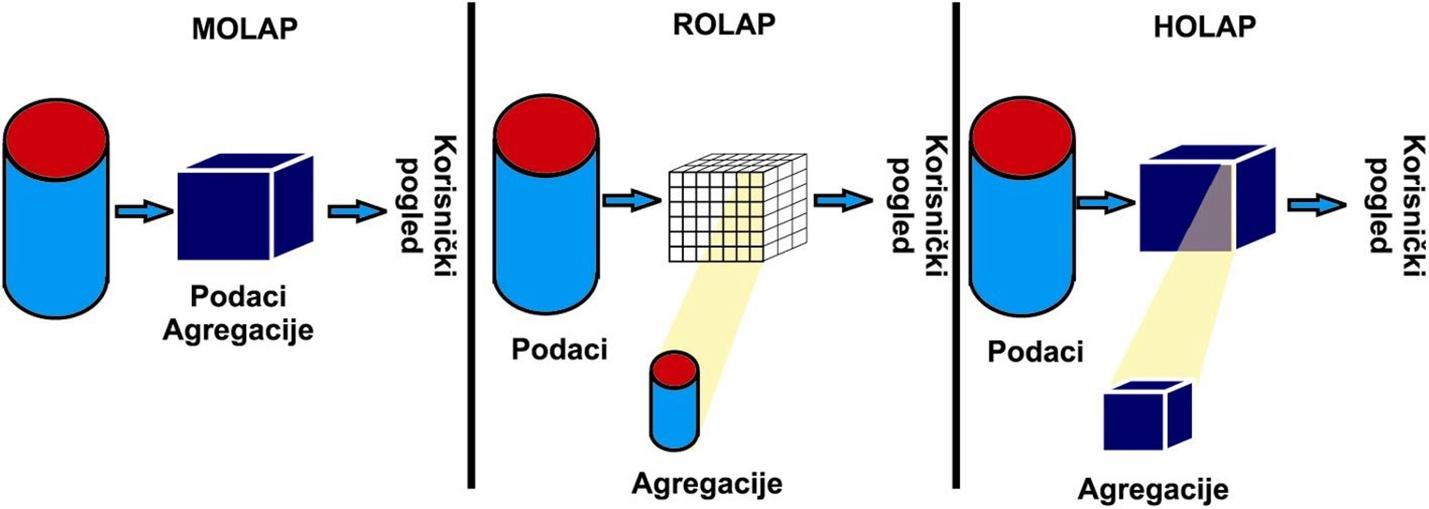
\includegraphics[width=0.85\linewidth]{slike/02/02-04.jpg}
    \caption{Типови OLAP коцки: MOLAP, HOLAP и ROLAP}
    \label{fig:02-27}
\end{figure}

\subsection{Изградња складишта података}
У овој секцији ће бити разматран развој складишта података. Две методологије — повезане са Вилијамом Инмоном (William Inmon) и Ралфом Кимбалом (Ralph Kimball) — доминирају овом облашћу већ три деценије. Иако наизглед супротстављене, ове методологије заправо имају исте циљеве, али их остварују на различите начине у зависности од контекста потреба за аналитичким захтевима.

\subsubsection{EDW и центри података}
\textbf{\textit{Enterprise data warehouse}} (EDW) је централизовано аналитичко складиште које интегрише структуриране податке из више изворних система широм организације и подржава извештавање и аналитику за предузеће у целини. Оно задовољава све четири Инмонове особине (§2.2.3.1) и служи, језиком који се понекад користи у пракси, као „single source of truth for management decisions”: један консолидован скуп података над којим се свако одељенско или међуфункционално питање може доследно решити (Inmon, 2005).

\textbf{\textit{Центар података}} (енг. \textit{data mart}) је тематски подскуп складишта, усмерен на једну пословну функцију — продају, финансије, људске ресурсе, маркетинг, CEO, CTO итд. — и оптимизован за упите које корисници те функције заиста извршавају (Kimball \& Ross, 2013). Продајни центар података садржи димензије и чињенице релевантне за анализу продаје (FACT\_SALES, DIM\_DATE, DIM\_PRODUCT, DIM\_CUSTOMER, DIM\_GEOGRAPHY) и подржава извештаје као што су приход по региону, најпродаванији производи и учинак продајних представника. Финансијски центар података садржи FACT\_GENERAL\_LEDGER и FACT\_BUDGET уз DIM\_ACCOUNT, DIM\_COST\_CENTER, DIM\_DATE и DIM\_LEGAL\_ENTITY, и подржава извештаје као што су поређење буџета и остварења по центру трошка, месечни P\&L и трендови обртног капитала. Производни центар података садржи FACT\_PRODUCTION\_OUTPUT и FACT\_DOWNTIME уз DIM\_PLANT, DIM\_PRODUCTION\_LINE, DIM\_PRODUCT, DIM\_SHIFT и DIM\_DATE, и подржава извештаје као што су број произведених јединица по смени, стопа шкарта по линији и узроци застоја по погону. Сваки центар података обликован је питањима која његови корисници заиста постављају.

Мартови постоје из четири разлога:

\begin{itemize}
  \item Прво, они нуде брже перформансе упита за своју циљну тематску област јер садрже само релевантне податке и могу бити уско подешени.
  \item Друго, они дају одељењу контролу над сопственим моделом података — дефиницијама мера, грануларношћу, SCD политикама — без потребе за сагласношћу читаве организације.
  \item Треће, лакши су за одржавање од једног монолитног складишта, јер се промене у једном марту не преносе ван његовог опсега.
  \item Четврто, поједностављују безбедност и контролу приступа: сваки март је ограничен на једну пословну функцију, па се привилегије засноване на улогама могу додељивати на нивоу марта — корисници финансија приступају финансијском марту, HR корисници HR марту — без излагања података ван њиховог домена.
\end{itemize}
Ово покреће основно питање: како су EDW и мартови међусобно повезани? Могућа су два одговора. По Инмоновом схватању, EDW се гради прво као јединствено интегрисано складиште, а мартови се из њега изводе као тематски усмерени подскупови. По Кимбаловом схватању, мартови се граде прво, један пословни процес у датом тренутку, и заједно чине складиште — повезани заједничким (conformed) димензијама. Ова два виђења воде ка две различите методологије, два различита артефакта планирања и два различита низа корака рада, који се развијају у наредна два пододељка.

\subsubsection{Инмонов приступ}
Инмонов приступ полази од идеје да се најпре изгради једно централно складиште за целу организацију, а да се тек после из њега изводе ужи центри података за поједина одељења (Inmon, 2005; Inmon, Strauss, \& Neushloss, 2008). Једноставно речено: прво се прави велика, заједничка основа, па се из ње праве специјализовани прикази за продају, финансије, људске ресурсе и друге функције.

Суштина овог приступа је у томе што се интеграција ради рано и централизовано. Предност је јасна: ако сви каснији мартови настају из истог централног модела, онда је лакше одржати доследност између њих. Мана је такође јасна: потребно је више времена и договора пре него што корисници виде прве конкретне резултате.

Предности овог приступа следе непосредно. Доследност између мартова загарантована је конструкцијом, а не дисциплином. Интеграциони слој у 3NF-у прихвата промене шеме и нове изворне системе без потребе за редизајном мартова, јер су мартови пројекције, а не примарна складишта. Могућност ревизије је снажна, јер интеграциони слој при сваком учитавању бележи пуно интегрисано стање пословања. Слабости су подједнако непосредне. Време до прве испоруке је дуго, јер се пословању ништа не испоручује док се модел на нивоу предузећа не изгради и из њега не изведе бар један март. Методологија је осетљива на почетни трошак моделовања: лоше процењен модел скупо је ревидирати. Уз то, овај приступ је слабо прилагођен организацијама чији се пословни процеси мењају брже од циклуса изградње складишта (Kimball \& Ross, 2013, ch. 1).

\begin{figure}[h]
    \centering
    
\includegraphics[width=0.85\linewidth]{slike/02/02-16.png}
    \caption{Инмонова архитектура одозго надоле (енг. top-down): изворни системи напајају ETL процес који учитава нормализовано 3NF складиште на нивоу предузећа (енг. enterprise data warehouse)}
    \label{fig:02-28}
\end{figure}

\subsubsection{Кимбалов приступ}
Кимбалов приступ иде обрнутим редом: најпре се граде појединачни центри података, један по један, а они заједно временом чине шире складиште (Kimball \& Ross, 2013; Kimball, Ross, Thornthwaite, Mundy, \& Becker, 2008). Уместо једног великог централизованог модела на самом почетку, нагласак је на томе да се брже испоруче конкретна решења за поједине пословне потребе. Да би такви центри ипак могли да раде заједно, деле исте кључне димензије, на пример датум, производ или купца.

\begin{figure}[h]
    \centering
    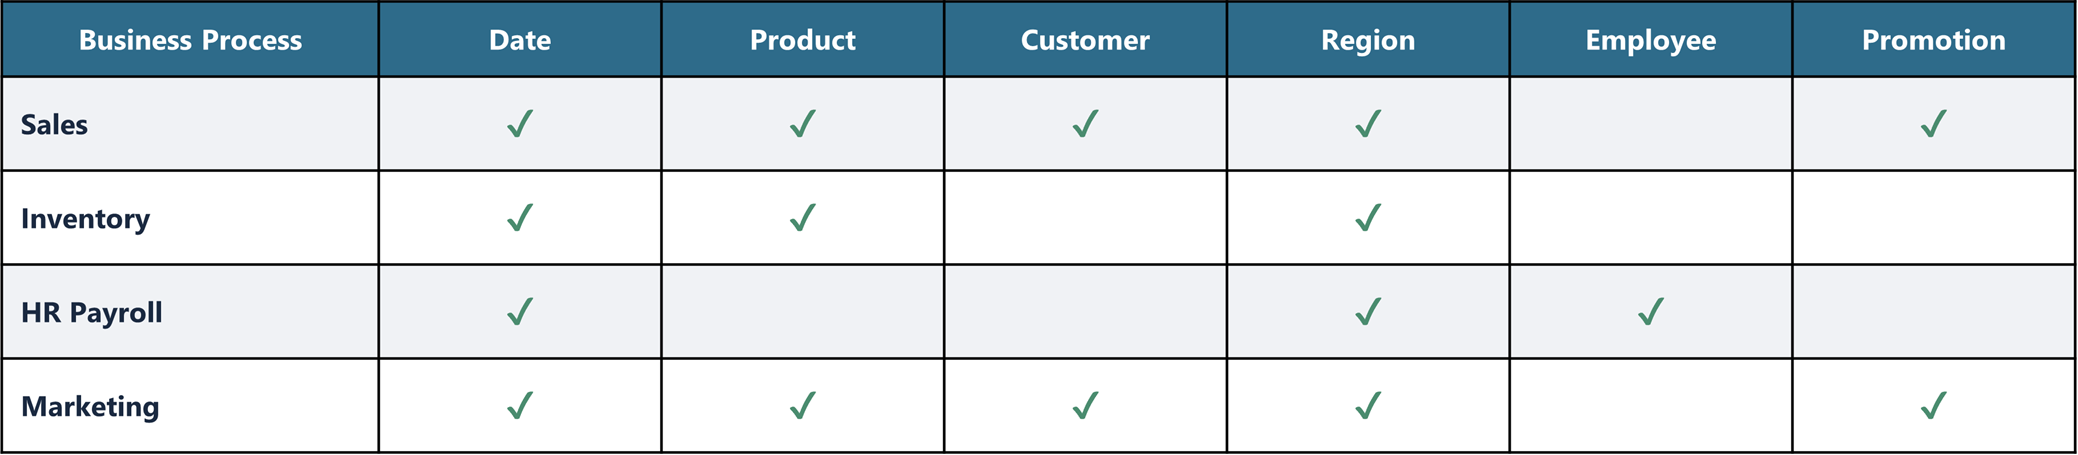
\includegraphics[width=0.85\linewidth]{slike/02/02-03.png}
    \caption{Кимбалова сабирничка матрица (енг. bus matrix): редови су пословни процеси, колоне су усаглашене димензије (енг. conformed dimensions)}
    \label{fig:02-29}
\end{figure}

Практичан алат за планирање у овом приступу јесте сабирничка матрица. Њена идеја је једноставна: у једној табели се бележи који пословни процеси користе које заједничке димензије. Тако тим лакше види шта може да се гради прво и које делове модела више мартова морају делити ако желимо да бројеви касније остану упоредиви.

Архитектура која из тога настаје назива се Кимбалова сабирница (енг. \textit{Kimball bus}): скуп димензионих мартова повезаних кичмом усаглашених димензија (енг. \textit{conformed dimensions}). Сабирница није засебна физичка структура већ дизајнерска дисциплина — мартови су физички одвојене табеле чињеница које се једноставно референцирају на идентично дефинисане димензионе табеле. План увођења мартова илустрован у изворној презентацији је типичан: Фаза 1 гради продајни март, са DIM\_DATE, DIM\_PRODUCT, DIM\_CUSTOMER и DIM\_GEOGRAPHY као усаглашеним димензијама; Фаза 2 гради финансијски март, поново користећи DIM\_DATE, DIM\_CUSTOMER и DIM\_GEOGRAPHY и додајући DIM\_ACCOUNT и DIM\_COST\_CENTER; Фаза 3 гради март људских ресурса, поново користећи DIM\_DATE и DIM\_GEOGRAPHY и додајући DIM\_EMPLOYEE и DIM\_DEPARTMENT. Редослед је вођен пословним приоритетом и зависношћу мартова од већ изграђених усаглашених димензија.

Мини-пример показује зашто су усаглашене димензије суштинске. Замислимо два марта: продајни март, чија табела чињеница бележи приход, количину и број трансакција, и маркетиншки март, чија табела чињеница бележи трошак кампање, број приказа и број кликова. Ако оба марта деле исте DIM\_DATE и DIM\_CUSTOMER табеле, аналитичар може да постави питање: колики је приход по сегменту купаца у месецима у којима је маркетиншка потрошња расла? Одговор је могућ само ако „месец” и „сегмент купца” значе исто у оба марта. Ако продаја користи сопствену верзију датума и сопствену поделу купаца, а маркетинг неку другу, поређење престаје да буде поуздано. Зато Кимбалова архитектура не тврди само да мартови треба да постоје, већ да морају бити повезани кроз исте димензије ако желимо интегрисано аналитичко окружење.

Предности овог приступа су обрнуте Инмоновим слабостима. Време до прве испоруке је кратко, јер се сваки март гради и уводи независно, а први март је у рукама корисника за неколико месеци, а не година. Итеративни ритам је боље прилагођен организацијама чији се приоритети мењају. Димензиона шема је читљива пословним корисницима и BI алатима, што и смањује терет обуке корисника и убрзава изградњу контролних табли и извештаја.

Слабости су обрнуте Инмоновим предностима. Доследност између мартова постиже се дисциплином, а не конструкцијом: ако је управљање усаглашеним димензијама слабо, два марта могу се разићи, а складиште губи своју интегративну улогу. Упити кроз процесе који обухватају више мартова зависе од тога да кључеви усаглашених димензија буду идентични у свима њима, што захтева трајну организациону посвећеност сабирничкој дисциплини (енг. \textit{bus discipline}) (Inmon, 2005).

\subsubsection{Поређење приступа}
Ни један ни други приступ није „једини исправан”. Корисније је питати у којој ситуацији је који приступ погоднији (Inmon et al., 2008; Kimball \& Ross, 2013). Оба имају исти циљ — поуздано аналитичко складиште — али до њега долазе различитим редоследом корака. Избор зато зависи од тога да ли је организацији важнија брза прва испорука или јача централна контрола модела од самог почетка.

Инмонов приступ је боље прилагођен организацијама које су велике, регулисане и стабилне: мултинационална банка, национална здравствена служба, велико комунално предузеће. Улагање у enterprise 3NF модел оправдано је ценом недоследности, регулаторним нагласком на могућност ревизије и дугим хоризонтом током којег ће складиште бити у употреби.

Кимбалов приступ је боље прилагођен организацијама које морају брзо да испоруче вредност, чији се процеси мењају у ритму месеци, а не година, и чија организација управљања може да одржи дисциплину усаглашених димензија: трговац, компанија која послује као услуга (енг. \textbf{\textit{software as a service}}), медијско предузеће. Већина предузећа налази се негде између ових полова, због чега је хибридни образац из §2.2.4.6 постао практични подразумевани избор.

Још два запажања су важна за избор. Прво, методологије се најоштрије разилазе око интеграционог слоја (3NF код Inmon-а, димензионо кроз усаглашене димензије код Kimball-а), а најмање око онога што корисник на крају упитује: у оба случаја, кориснички слој је димензиони. Друго, ниједна методологија, како је првобитно дефинисана, не обрађује изворно облачне, ELT-вођене архитектуре језерског складишта (енг. \textit{cloud-native}, \textit{ELT-driven}, \textit{lakehouse style}) које су се појавиле током последње деценије; њима се бави §2.2.4.8. Методологије остају корисне као концептуални оквири чак и тамо где је имплементациона технологија одмакла, јер су архитектонска питања која постављају — где интегрисати, како управљати заједничким димензијама, како управљати временски варијантном променом — иста питања на која свака аналитичка платформа мора да одговори.

\subsubsection{Референтна архитектура}
Без обзира на то да ли се складиште гради одозго надоле или одоздо нагоре, иста трослојна референтна архитектура организује ток података од извора до корисника (Слика~\ref{fig:02-30}). Сваки слој има посебну улогу, посебне гаранције квалитета и посебан скуп корисника; границе између слојева су места на којима се примењују трансформације и на којима се спроводи могућност ревизије складишта (Kimball \& Ross, 2013; Inmon et al., 2008).

\begin{figure}[h]
    \centering
    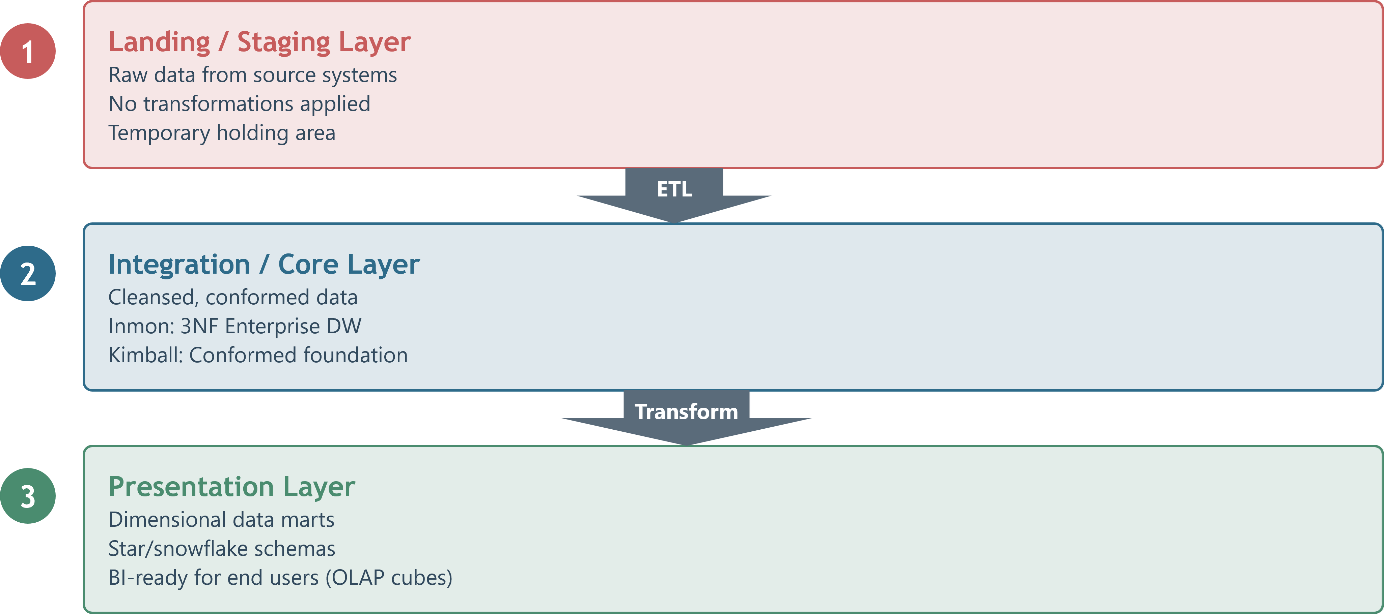
\includegraphics[width=0.85\linewidth]{slike/02/02-09.png}
    \caption{Трослојна референтна архитектура: прихватни слој (енг. staging), интеграциони слој (енг. integration) и презентациони слој (енг. presentation)}
    \label{fig:02-30}
\end{figure}

\textbf{\textit{Прихватни слој}} (енг. \textit{staging}) садржи сирове податке издвојене из изворних система. Подаци се учитавају суштински онако како су стигли — у изворним форматима, са изворним називима атрибута, са свим проблемима квалитета који су постојали на извору — и чувају се само онолико дуго колико захтева следећи циклус учитавања. Тај слој има две сврхе. Прво, изолује процес учитавања у складиште од изворних система: издвајање се може завршити у уском оперативном прозору, а спорије трансформације могу се независно извршавати над прихватном копијом без даљег оптерећења извора. Друго, обезбеђује контролну тачку за поновно покретање и опоравак: ако корак трансформације не успе, ETL процес се може наставити из прихватног слоја без поновног издвајања са извора.

\textbf{\textit{Интеграциони (или језгарни, енг. core)}} слој је место где се успоставља идентитет складишта. Подаци из прихватног слоја (енг. \textit{staging}) се чисте, стандардизују, усклађују са канонским форматима и помирују између извора; додељују се сурогатни кључеви (енг. \textit{surrogate keys}); примењује се SCD логика; спроводи се референтни интегритет (енг. \textit{referential integrity}). У Инмоновој методологији овај слој је enterprise 3NF складиште, јединствени извор истине из којег се изводе мартови. У Кимбаловој методологији овај слој је од почетка димензиони, са усаглашеним димензијама (енг. \textit{conformed dimensions}) и fact табелама изграђеним директно. У оба случаја, интеграциони слој је ниво на којем складиште задовољава Инмонове четири особине: тематски је оријентисано у својој организацији, интегрисано кроз изворе, неиспарљиво и временски варијантно.

\textbf{\textit{Презентациони слој}} (енг. \textit{presentation layer}) је оно што BI алати и крајњи корисници заправо упитују. Његове табеле су димензионе — звездасте или галаксијске шеме (енг. \textit{star} или \textit{galaxy schema}) — и подешене су за перформансе читања: агрегатне табеле (енг. \textit{aggregate tables}), материјализовани погледи (енг. \textit{materialized views}), колонарни индекси (енг. \textit{columnar indexes}) и, где се користе, OLAP коцке изграђене директно над димензионом шемом. Презентациони слој може бити засебна физичка структура (скуп мартова изведених из интеграционог слоја) или логички слој погледа над интеграционим слојем; избор је једна од дизајнерских одлука које разматра §2.2.4.6. Из перспективе корисника, презентациони слој јесте складиште: то је извор на који се контролна табла повезује и структура коју пивот табела чита.

Кроз сва три слоја протежу се две архитектонске дисциплине. Прва су метаподаци: свака табела, свака колона и свака трансформација документовани су у репозиторијуму метаподатака, тако да се порекло података (енг. \textbf{\textit{lineage}}) од извора преко прихватног, интеграционог и презентационог слоја може пратити. Порекло података је оно што складиште чини одбрањивим пред ревизорима, подложним отклањању грешака када је неки број погрешан и одрживим када се изворни системи мењају. Друга је праћење квалитета података: граница између прихватног и интеграционог слоја је природно место за примену правила квалитета (потпуност, јединственост, провере домена вредности), преусмеравање спорних редова у карантинску табелу (енг. \textbf{\textit{quarantine table}}) и упозоравање оперативног тима на систематске проблеме. §2.2.4.7.7 развија праксе квалитета података и профилисања кроз које се ове дисциплине операционализују.

\subsubsection{Хибридна пракса}
Већина организација значајне величине не спроводи ниједну методологију у чистом облику. Практични подразумевани образац најбоље је разумети као слојевиту референтну архитектуру из §2.2.4.5, у којој је сваком слоју додељена најприкладнија методологија. Тај образац комбинује предности оба приступа (Inmon et al., 2008; Kimball \& Ross, 2013). Интеграциони слој гради се у Инмоновом стилу: као нормализовани 3NF модел који обухвата интегрисано стање пословања, подржава могућност ревизије и отпоран је на промене у димензионим пројекцијама изграђеним изнад њега. Презентациони слој гради се у Кимбаловом стилу: као скуп димензионих мартова са усаглашеним димензијама, оптимизованих за употребу BI алата и за упите које корисник заиста извршава.

Хибридни образац разрешава централну напетост између ове две методологије. 3NF интеграциони слој гарантује доследност конструкцијом — сваки март је изведен из истог интегрисаног модела, па се дисциплина усаглашених димензија спроводи архитектонски, а не организационо. Истовремено, димензиони презентациони слој испоручује перформансе упита, читљивост шеме и компатибилност са BI алатима до којих је кориснику стало. Цена овог обрасца је то што се подаци материјализују два пута — једном у интеграционом слоју, једном у презентационом слоју — и ETL цевовод (енг. \textbf{\textit{ETL pipeline}}) мора да трансформише из 3NF у димензиони облик. У савременим изворно облачним складиштима тај трошак је подношљив, јер је складиштење јефтино, а димензиона пројекција може се имплементирати као погледи или као материјализације на захтев, а не као потпуно дуплиране табеле.

Хибридни образац такође прихвата даља архитектонска проширења која су ушла у праксу откако су канонске методологије успостављене. Data Vault 2.0 (Linstedt \& Olschimke, 2015), разматран у §2.2.4.8.1, природно стоји као алтернатива 3NF-у у интеграционом слоју: чува својства могућности ревизије која Инмонов приступ цени, уз боље прилагођавање честим променама шеме и паралелном учитавању него што то омогућава 3NF модел. Изворно облачна складишта (Snowflake, BigQuery, Redshift, Azure Synapse), разматрана у §2.2.4.8.3, мењају имплементациону технологију сваког слоја без промене саме слојевите структуре: складиштење и рачунарски ресурси су раздвојени, скалирање је еластично, а ELT образац из §2.2.4.7.6 помера тежак трансформациони рад са засебног ETL механизма на сопствени SQL механизам складишта. Архитектура језерског складишта (енг. \textit{lakehouse}) (Armbrust, Ghodsi, Xin, \& Zaharia, 2021), разматрана у §2.2.4.8.2, раствара границу између прихватног и интеграционог слоја тако што омогућава да сирови и курирани подаци коегзистирају у истом слоју складиштења са ACID семантиком. Ниједно од ових проширења не поништава слојевиту референтну архитектуру; свако мења физички изглед једног или више слојева, задржавајући њихову логичку улогу.

Општа поука је да методологија служи архитектонској потреби, а не обрнуто (Inmon et al., 2008). Студенту основних студија више користи разумевање слојевите архитектуре, методологија које се могу доделити сваком слоју и компромиса које свака таква додела подразумева, него третирање било Инмона (Inmon) било Кимбала (Kimball) као потпуног и самодовољног рецепта. Следећи пододељак прелази на интеграциони механизам који повезује слојеве — ETL или ELT цевовод — и разрађује га у дубини коју његов оперативни значај оправдава.

\subsubsection{ETL и ELT}
Екстракција, трансформација и учитавање (енг. \textit{extract-transform-load}, ETL) јесте процес којим се подаци крећу из изворних система преко прихватног слоја (енг. \textit{staging}) у интеграциони и презентациони слој складишта. То је истовремено оперативно најзначајнија и најпотцењенија компонента програма изградње складишта података: студије напора при имплементацији складишта редовно сврставају развој ETL-а на шездесет до осамдесет процената укупне цене пројекта (Kimball, Caserta, \& Mundy, 2008), а поузданост сваког извештаја и контролне табле које складиште служи зависи од исправности ETL цевовода (енг. \textit{ETL pipeline}) који је учитао основне табеле. Овај пододељак разматра сваку од три фазе редом, а затим испитује оркестрацију, разлику ETL/ELT и дисциплину квалитета података која се протеже кроз све фазе.

\textbf{\textit{Екстракција}} (енг. \textit{extraction}) јесте повезивање процеса учитавања у складиште са изворним системима. Извори су хетерогени: релационе базе података (SQL Server, Oracle, PostgreSQL), равне датотеке (енг. \textbf{\textit{flat files}}; CSV, fixed-width, Excel), пакетиране пословне апликације са сопственим интерфејсима за извоз, REST API-ји који враћају JSON, токови порука (енг. \textbf{\textit{message streams}}) и — у старијим организацијама — mainframe скупови података којима се приступа преко наменских конектора. Компонента издвајања у ETL цевоводу мора да прихвати сваки од ових типова извора и изолује остатак цевовода од њихових особености (Kimball et al., 2008).

Две стратегије екстракције су у уобичајеној употреби:

\begin{itemize}
  \item \textbf{\textit{Потпуно издвајање}} (енг. \textit{full extraction}) копира читав изворни скуп података при сваком покретању; једноставно је за имплементацију и отпорно на промене шеме изворног система, али се слабо скалира када су изворне табеле велике, а стопа промене мала.
  \item \textbf{\textit{Инкрементално издвајање}} (енг. \textit{incremental extraction}) копира само редове који су се променили од претходног покретања; то је доминантна стратегија у производним складиштима и оперативно место на коме заправо живи највећи део ETL сложености (Kimball et al., 2008).
\end{itemize}
Унутар инкременталног издвајања користе се три механизма за идентификацију промењених редова. Први су временски жигови као водене линије: изворна табела носи временски жиг последње измене, а свако издвајање тражи редове измењене након ознаке највише достигнуте вредности (енг. \textbf{\textit{high-water mark}}) из претходног покретања. Други је хватање промена у подацима (енг. \textbf{\textit{change-data capture}}, CDC): сам механизам изворне базе података бележи промене на нивоу реда (у PostgreSQL-у кроз логичку репликацију, у SQL Server-у кроз CDC функцију, у Oracle-у кроз GoldenGate), а процес издвајања конзумира тај лог. Трећи су заставице промене: апликација експлицитно означава редове као нове или измењене, а процес издвајања чисти заставицу након конзумирања.

CDC је пожељан за OLTP изворе великог обима јер бележи сваку промену на нивоу базе без измене апликације или ослањања на тачност временских жигова; водене линије су довољне за једноставније изворе где је обим умерен, а шема под контролом тима за складиште. Избор механизма није академски — он одређује шта ће складиште видети, а шта неће. Водена линија заснована на временском жигу пропушта брисања (обрисани ред нема преживели временски жиг по коме би се филтрирао); CDC их хвата. Заставица промене зависи од дисциплине апликације која временом може ослабити. Extraction дизајн мора бити усклађен са стварним понашањем изворног система, а усклађеност се мора поново преиспитати кад год се извор промени.

Четири оперативна ограничења обликују фазу издвајања. Прво, прозори доступности изворног система: производни OLTP системи не смеју бити успоравани издвајањем током радног времена, а издвајање мора бити завршено у дефинисаном ноћном или сатном прозору. Друго, права приступа и безбедност: није свака колона у извору одобрена за издвајање, а лично препознатљиви или регулисани подаци могу захтевати редакцију или псеудонимизацију на граници. Треће, неусаглашеност формата међу изворима: исти логички атрибут може стићи са различитим типовима, кодирањима, раздвајачима или представама null вредности из сваког извора, а компонента за издвајање мора сваки од њих да ухвати у облику који фаза трансформације може да обради. Четврто, мрежна латенција код удаљених и облачних извора: издвајање преко мреже ограничено је расположивом пропусношћу и толеранцијом на латенцију процеса који конзумира, што обоје ограничава колико агресивно инкрементално издвајање може бити постављено.

\textbf{\textit{Трансформација}} (енг. \textit{transformation}) је фаза у којој се издвојени подаци преобликују у канонски облик који складиште користи. Рад трансформације распада се на низ операција, од којих свака решава једну класу разлике између извора и одредишта (Kimball et al., 2008). Стандардни низ је прихватни слој (енг. \textit{staging}) → чишћење (енг. \textit{cleansing}) → стандардизација (енг. \textit{standardization}) → примена пословних правила (енг. \textit{application of business rules}) → генерисање кључева (енг. \textit{key generation}) → уклањање дупликата (енг. \textit{deduplication}) → припрема за интеграциони слој (енг. \textit{preparation for the integration layer}).

\textbf{\textit{Чишћење}} (енг. \textit{cleansing}) решава недостатке у изворним подацима. Null вредности морају бити обрађене — замењене подразумеваном вредношћу (нула, “непознато”, пословно дефинисано резервно решење), преусмерене у табелу одбијених редова (енг. \textbf{\textit{reject table}}) ради људског прегледа или учитане са колоном ознаке квалитета (енг. \textbf{\textit{quality flag}}) коју накнадни извештаји могу филтрирати. Неисправне вредности морају бити откривене и или исправљене према референтној листи или изоловане. Дупликатни редови морају бити идентификовани, било тачним поклапањем на кандидатском кључу или приближним поклапањем на атрибутима као што су имена и адресе тамо где се идентификатори изворних система не поклапају.

\textbf{\textit{Стандардизација}} (енг. \textit{standardization}) доводи сваку вредност у канонски облик. Датуми се претварају у ISO 8601 (“01/15/24”, “2024-01-15” и “Jan 15, 2024” сви постају 2024-01-15). Кодови држава се претварају у ISO 3166 (“US”, “USA” и “United States” сви постају US). Јединице мере се претварају у метрички систем (“kg”, “lbs” и “kilograms” сви постају kilograms у једној јединственој репрезентацији). Стандардизација је место где се интеграционо својство складишта — једнако значење подразумева једнаку репрезентацију, принцип наведен у §2.2.3.3 — оперативно спроводи.

\textbf{\textit{Примена пословних правила}} (енг. \textit{application of business rules}) је место на коме складиште спроводи логику организације за изведене мере и класификације. Израчунаване колоне — приход је количина пута цена, маржа је приход минус трошак, кашњење у данима је датум испоруке минус датум поруџбине — израчунавају се и чувају. Правила класификације — клијент високе вредности ако кумулативни приход прелази праг, касна испорука ако кашњење у данима прелази толеранцију — примењују се. Правила валидације — датум испоруке мора бити већи од датума поруџбине, клијент мора имати најмање осамнаест година — спроводе се, а редови који их крше преусмеравају се у карантинску табелу (енг. \textit{quarantine table}).

\textbf{\textit{Генерисање кључева}} (енг. \textit{key generation}) управља дисциплином сурогатног кључа (енг. \textit{surrogate key}) из §2.2.3.5.3. Природни кључеви (енг. \textit{natural keys}) из изворних система никада се не користе као примарни кључеви у складишту; уместо тога, сваки ред уметнут у димензиону табелу добија сурогатни кључ генерисан IDENTITY колоном или секвенцом, а сваки ред чињеница (енг. \textit{fact row}) повезује се са својим димензијама преко тих сурогатних кључева. Пресликавање кључева (енг. \textit{lookup}) које природни кључ из изворног система повезује са одговарајућим сурогатним кључем складишта јесте оперативно језгро учитавања димензија и место на коме се примењује SCD логика. Стандардни образац, извршен за сваки долазни изворни ред, гласи: пронађи природни кључ у димензионој табели; ако је ред нов, генериши нови сурогатни кључ и уметни; ако је ред непромењен, узми постојећи сурогатни кључ; ако је ред промењен, примени SCD стратегију декларисану за тај атрибут (затвори постојећи ред и уметни нови за тип 2, енг. \textit{Type 2}; препиши за тип 1, енг. \textit{Type 1}; ажурирај додатну колону за тип 3, енг. \textit{Type 3}); врати сурогатни кључ позиваоцу ради употребе у учитавању табеле чињеница (енг. \textit{fact-table loading}).

\textbf{\textit{Учитавање}} (енг. \textit{loading}) је уписивање трансформисаних података у складиште. Ова фаза има три тачке дисциплине: редослед учитавања, стратегију учитавања и обраду грешака.

Редослед учитавања ограничен је референтним интегритетом (енг. \textbf{\textit{referential integrity}}). Димензије морају бити учитане пре табела чињеница (енг. \textbf{\textit{fact tables}}) које их референцирају, јер су сурогатни кључеви додељени током учитавања димензија потребни учитавању табела чињеница ради попуњавања страних кључева. Стандардни редослед је прво табеле прихватног слоја (енг. \textbf{\textit{staging tables}}), затим димензионе табеле (са примењеном SCD логиком), па табеле чињеница (са пресликавањем сурогатних кључева, енг. \textbf{\textit{surrogate-key lookups}}, према управо учитаним димензијама). Обртање редоследа — учитавање чињеница пре димензија — производи редове чињеница чији страни кључеви још не постоје у димензионим табелама, нарушавајући референтни интегритет и кварећи сваки упит који спаја табелу чињеница и димензију. Ово ограничење је чврсто, а не саветодавно (Kimball et al., 2008).

Стратегија учитавања бира између потпуног поновног учитавања (енг. \textbf{\textit{full reload}}) и инкременталног дописивања и ажурирања (енг. \textbf{\textit{incremental upsert}}). Потпуно поновно учитавање празни циљну табелу и поново убацује сваки ред из прихватног слоја; једноставно је, отпорно на грешке у инкременталној логици и изводљиво за мале димензије, али брзо постаје неизводљиво за табеле чињеница са стотинама милиона редова. Инкрементално дописивање и ажурирање примењује MERGE операцију која убацује нове редове и ажурира промењене редове по примарном кључу; скалира се на веома велике табеле чињеница, али захтева дисциплину инкременталног издвајања описану на почетку овог одељка и осетљивије је на логичке грешке. У пракси се димензије типично потпуно поново учитавају (број њихових редова је довољно мали), а табеле чињеница се учитавају инкрементално.

Обрада грешака је место на коме се успоставља оперативна поузданост складишта. Одбачене датотеке (енг. \textbf{\textit{reject files}}) хватају редове који не прођу валидацију; карантинске табеле држе редове који пролазе валидацију али изазивају сумње у квалитет података; систем упозоравања (енг. \textbf{\textit{alerting}}) обавештава оперативни тим када стопе грешака пређу праг; стратегије враћања (енг. \textbf{\textit{rollback}}) омогућавају да се делимична учитавања врате када неки низводни корак не успе. Учитавање које откаже на пола пута може оставити складиште у недоследном стању — чињенице учитане уз делимично ажуриране димензије, или агрегате недоследне са основним детаљима — а опоравак из таквих стања скупљи је него њихово спречавање. Дисциплинован ETL цевовод третира свако учитавање као трансакциону целину: или се у потпуности заврши и потврди, или се враћа на претходно доследно стање.

\paragraph{Оркестрација и алати}
ETL цевовод није један програм већ граф зависних задатака: издвајање из сваког извора, кораци трансформације у низу, учитавања димензија, учитавања чињеница, освежавања агрегата и накнадна обавештења. Оркестрација је дисциплина заказивања ових задатака, спровођења њихових зависности, праћења њиховог извршења и опоравка од неуспеха. Четири појма оркестрације су стандардна (Kimball et al., 2008). Распоређивање (енг. \textbf{\textit{scheduling}}) одређује када се цевоводи извршавају — ноћно, сваки сат, на догађајне окидаче или као непрекидни токови. Управљање зависностима осигурава да се низводни задатак покрене тек након што сваки узводни задатак од кога зависи успешно заврши; ако било који узводни задатак не успе, зависни задаци се задржавају док се неуспех не разреши. Праћење (енг. \textbf{\textit{monitoring}}) бележи логове извршења, бројеве редова у свакој фази, трајања и стопе грешака, и излаже их и за оперативно упозоравање и за дугорочно планирање капацитета. Опоравак (енг. \textbf{\textit{recovery}}) дефинише логику поновног покретања: цевовод који откаже на пола пута мора бити могуће поново покренути из контролне тачке, а не од почетка, и оркестратор (енг. \textbf{\textit{orchestrator}}) мора да спроведе идемпотентност (енг. \textbf{\textit{idempotency}}) тако да поново покренути задатак не дуплира рад свог ранијег покушаја.

Четири породице алата доминирају оркестрационим пејзажом. SQL Server Integration Services (SSIS) је Microsoft-ова традиционална ETL платформа, тесно интегрисана са SQL Server екосистемом и широко примењена у организацијама стандардизованим на Microsoft технологији. Apache Airflow је оркестратор отвореног кода (енг. \textbf{\textit{open-source orchestrator}}) најшире усвојен у новим пројектима: цевоводи се дефинишу као Python усмерени ациклични графови (енг. \textbf{\textit{directed acyclic graphs}}, DAGs), инфраструктура за заказивање и праћење је зрела, а екосистем изворних конектора је велик. Talend нуди интеграциону платформу за велике организације, са графичким дизајнером цевовода и широком библиотеком конектора. Tableau Prep пружа уже фокусиран алат оријентисан ка припреми података коју воде аналитичари, а не ка ETL-у на нивоу предузећа. Избор између њих мање је вођен поређењем функционалности, а више постојећим технолошким стеком организације и профилом вештина тима који ће управљати цевоводом.

\paragraph{Пример од почетка до краја}
Дисциплина претходних пододељака постаје опипљива када се прати један продајни запис од извора до табеле чињеница. Пример испод репродукује разрађени цевовод из изворне презентације и репрезентативан је за оно што ETL цевовод мора да уради за један ред FACT\_SALES (Слика~\ref{fig:02-31}).

\begin{figure}[h]
    \centering
    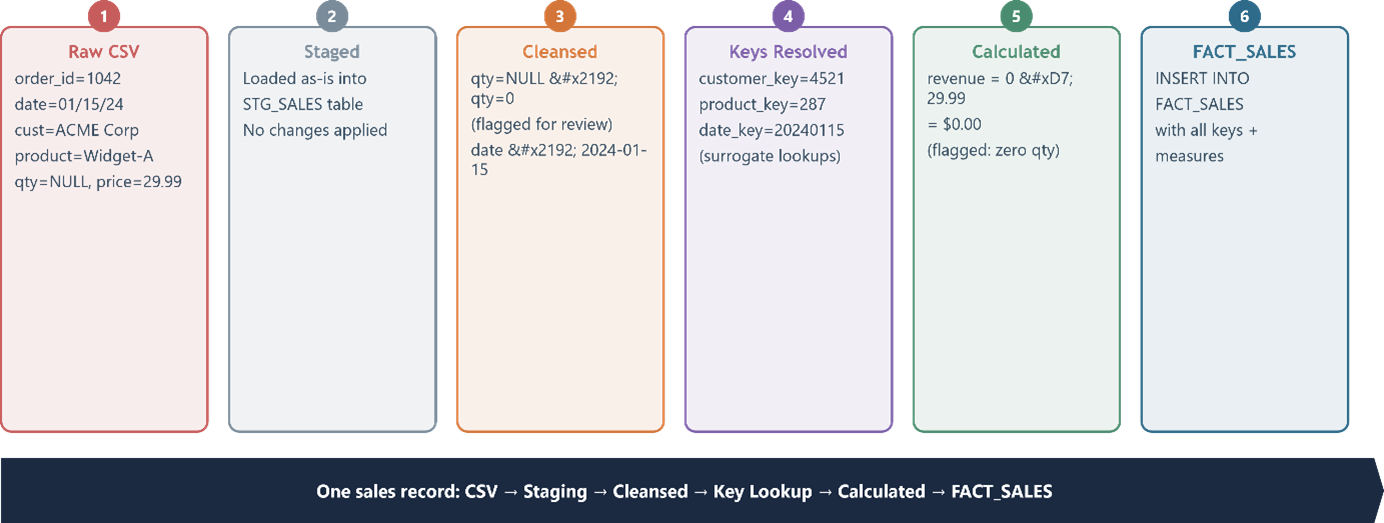
\includegraphics[width=0.85\linewidth]{slike/02/02-11.png}
    \caption{ETL цевовод (енг. ETL pipeline) од почетка до краја: један продајни запис праћен од сировог CSV-а до FACT\_SALES}
    \label{fig:02-31}
\end{figure}

CSV фајл из система за управљање поруџбинама стиже у прихватну област (енг. \textit{staging area}) са редом који садржи \texttt{order\_id = 1042}, \texttt{date = „01/15/24”}, \texttt{cust = „ACME Corp”}, \texttt{product = „Widget-A”}, \texttt{qty = NULL}, \texttt{price = 29,99}. Ред се учитава у прихватну табелу \texttt{STG\_SALES} тачно онако како је примљен, без примењене трансформације. У том тренутку складиште држи ред у изворном облику: сваки недостатак у изворној вредности очуван је дословно како би накнадно чишћење (енг. \textbf{\textit{cleansing}}) имало све доказе потребне за деловање.

Чишћење претвара поље датума из US формата “01/15/24” у канонски ISO 8601 облик 2024-01-15. Недостајућа количина (\texttt{NULL}) се замењује нулом и ред се означава за преглед у колони квалитета података; алтернатива — потпуно одбацивање реда — резервисана је за случајеве у којима је \texttt{NULL} структурно неважећи, а не поправљив недостатак. Даље промене се не примењују: називи купца и производа остају у облику природног кључа (енг. \textit{natural key}), чекајући пресликавање сурогатног кључа (енг. \textit{surrogate-key lookup}) у следећем кораку.

Разрешење сурогатног кључа тражи сваки природни кључ у одговарајућој димензионој табели. Купац “ACME Corp” налази се у \texttt{DIM\_CUSTOMER} и враћа \texttt{customer\_sk = 4521} (његову текућу верзију типа 2, енг. \textit{Type 2}). Производ “Widget-A” налази се у \texttt{DIM\_PRODUCT} и враћа \texttt{product\_sk = 287}. Очишћени датум 2024-01-15 налази се у \texttt{DIM\_DATE} и враћа \texttt{date\_sk = 20240115}. Да се неки од природних кључева није поклопио, ред би био преусмерен у карантинску табелу; у овом примеру сва три се уредно разреше.

\textbf{\textit{Примена пословних правила}} (енг. \textit{application of business rules}) израчунава изведене мере које табела чињеница захтева. Приход се израчунава као количина пута цена: у овом случају, нула пута 29,99 једнако је 0,00 RSD. Ред се означава у посебној колони да покаже да вредност нултог прихода потиче од недостатка у пољу количине, а не од стварне трансакције са нултим приходом. Ова разлика је важна за накнадно извештавање: контролна табла која агрегира приход треба да укључи ред као нулу (како би се укупни износи усагласили), али треба и да прикаже број ознака недостатака како би проблеми квалитета података били видљиви.

Завршни корак убацује ред у FACT\_SALES који носи три сурогатна кључа (енг. \textit{surrogate keys}), очишћене и израчунате мере (qty = 0, price = 29,99, revenue = 0,00) и ознаке квалитета података. Ред је сада део интегрисаног, временски обележеног записника продајног процеса заснованог на сурогатним кључевима. Упит контролне табле који агрегира приход по купцу и месецу дохватиће овај ред преко његових date\_sk и customer\_sk и комбиновати га са сваком другом продајом тог периода; ред ће се моћи ускладити са својим изворним CSV-ом преко order\_id, који је очуван као дегенерисана димензија на fact табели.

\paragraph{ETL насупрот ELT}
До отприлике 2015. године стандардни образац је недвосмислено био ETL: подаци су се издвајали из извора, трансформисали засебним механизмом (SSIS, Informatica, Talend) и учитавали у складиште већ у свом коначном облику. Механизам трансформације био је засебан део инфраструктуре са сопственим рачунарским ресурсима и сопственим карактеристикама скалирања. Овај образац је добро одговарао локално постављеним складиштима (енг. \textbf{\textit{on-premises}} warehouses) са ограниченим рачунарским капацитетом, где је резервисање ресурса складишта за радно оптерећење упита и измештање трансформације у засебан механизам било архитектонска нужност.

Пораст изворно облачних складишта — Snowflake, BigQuery, Redshift, Azure Synapse — променио је ограничење. Облачна складишта раздвајају складиштење од рачунарских ресурса и нуде еластичне ресурсе који се наплаћују по упиту (енг. \textbf{\textit{pay-per-query}}) и који се на захтев скалирају на огромна оптерећења. У овом режиму трансформација се може изводити унутар самог складишта употребом његовог сопственог SQL механизма, при чему се сирови подаци прво учитавају у складиште, а трансформације примењују као SQL искази над учитаним табелама. Тај образац назива се ELT — издвоји, учитај, трансформиши (енг. \textit{extract, load, transform}). Подаци се учитавају у складиште у сировом или скоро сировом облику; трансформациони рад се изражава као SQL, често слојевито преко алата као што је dbt који додаје управљање верзијама (енг. \textit{version control}), тестирање (енг. \textit{testing}) и управљање зависностима (енг. \textit{dependency management}); еластични рачунарски ресурси складишта скалирају се и на трансформационо и на упитно оптерећење. Помак ка ELT-у био је једна од најзначајнијих архитектонских промена последње деценије и у великој мери је демократизовао изградњу складишта, уклањањем потребе за посебним ETL механизмом и специјализованим вештинама потребним за његово одржавање.

Избор између ETL-а и ELT-а сада је питање усклађености, а не могућности. ELT је природан избор за изворно облачна складишта са еластичним рачунарским ресурсима, за организације које преферирају SQL-засновану трансформациону логику уместо цевовода графичких алата и за пројекте где је време до прве вредности важније од изолације инфраструктуре. ETL остаје прави избор за осетљиве податке који морају бити очишћени пре него што буду трајно уписани у складиште, јер сами сирови, неочишћени подаци могу бити регулаторни или безбедносни проблем, за локално постављена складишта где су рачунарски ресурси ограничени и за организације чије је постојеће улагање у ETL алате велико. dbt — SQL-first оквир за трансформацију који је сада фактички стандард (енг. \textbf{\textit{de facto standard}}) за ELT цевоводе на облачним складиштима — био је главни убрзивач усвајања ELT-а отприлике од 2018. године.

\paragraph{Квалитет података и профилисање}
Квалитет података је дисциплина која осигурава да складиште испоручује тачне, потпуне, доследне и благовремене податке својим корисницима; она се спроводи кроз профилисање, правила квалитета и континуирано праћење (Kimball et al., 2008). Профилисање је систематско испитивање изворних података пре него што буду моделовани или учитани: потпуност колона (удео null вредности), расподела вредности (табеле фреквенција за категоријалне атрибуте, сумарне статистике за нумеричке атрибуте), откривање образаца (усаглашеност са регуларним изразима за поља као што су email и поштански број), анализа јединствености (да ли су кандидатски кључеви заиста јединствени) и провере доследности између извора (да ли исти купац у два система носи атрибуте који се могу помирити). Аргумент за профилисање, изречен без увијања од стране практичара који су га развили, јесте да складиште не може бити исправно моделовано док се не разуме стварни облик његових изворних података — а стварни облик ретко је оно што тврди изворна документација.

Правила квалитета, примењена током фаза чишћења и валидације у трансформацији, кодирају очекивања организације о њеним подацима. Правила се крећу од једноставних (старост купца мора бити позитивна, код државе мора постојати у ISO 3166) до сложених (уплата мора да се помири са отвореним рачуном у оквиру толеранције). Свако правило има дефинисан одговор када је прекршено: одбаци ред, преусмери га у карантин, учитај га са ознаком квалитета (енг. \textbf{\textit{quality flag}}) или упозори оператера. Избор одговора сам по себи је одлука квалитета података и бележи се у метаподацима складишта.

\textbf{\textit{Праћење}} (енг. \textit{monitoring}) затвара петљу. Правила квалитета која пролазе у време моделовања могу почети да отказују како се изворни системи развијају; профилисање које је било тачно пре годину дана можда више не одражава податке које извор данас производи. Зрела пракса управљања складиштем непрекидно извршава правила квалитета, прати стопе пролаза кроз време и упозорава оперативни тим када стопе падну испод прага или када новоуведена правила открију раније немоделоване недостатке. Ово је оперативна манифестација принципа да квалитет није својство једног учитавања, већ својство складишта као непрекидно еволуирајућег система.

\subsubsection{Савремени правци}
Методологије Инмона и Кимбала успостављене су између касних 1980-их и раних 2000-их, када су складишта била локално постављена (енг. \textbf{\textit{on-premises}}), рачунарски ресурси и складиштење били тесно повезани, а изворни системи бројали десетине. Архитектонски пејзаж се од тада значајно променио. Три развоја ушла су у праксу током последње деценије и сада су стандардни делови сваке савремене расправе: Data Vault 2.0 као алтернативни образац моделовања интеграционог слоја, језерско складиште (енг. \textbf{\textit{lakehouse}}) као архитектонска фузија језера података (енг. \textbf{\textit{data lake}}) и складишта, и изворно облачна складишта (енг. \textbf{\textit{cloud-native warehouses}}) као доминантна платформа за распоређивање. Овај пододељак разматра сваки од њих у сажетом облику, уз кратак преглед даљих трендова — интеграције AI/ML-а, data mesh-а и аналитике токова података — који обликују пејзаж складишта крајем 2020-их.

\paragraph{Data Vault 2.0}
Data Vault 2.0, који је увео Ден Линстед (Dan Linstedt) почетком 2000-их и кодификован у раду Линстеда и Олшимајкеа (Linstedt \& Olschimke, 2015), алтернативни је образац моделовања интеграционог слоја складишта. Док Инмонов 3NF модел хвата пословна правила у шеми, а Кимбалов димензиони модел их хвата у усаглашеним димензијама, Data Vault у потпуности раздваја структурне и дескриптивне бриге шеме. Модел чине три типа табела: чворишта (енг. \textit{hubs}) држе јединствене пословне кључеве за сваки субјект (купац, производ, поруџбина); везе (енг. \textit{links}) држе односе између чворишта; а сателити (енг. \textit{satellites}) држе описне атрибуте који описују чвориште или везу, при чему је сваки сателит означен временом учитавања тако да се историја акумулира додавањем редова, а не ажурирањем постојећих.

Посебна својства овог обрасца следе из тог раздвајања. Могућност ревизије је структурна: сваки ред носи изворни систем и време учитавања, а свако историјско стање сваког ентитета може се реконструисати избором satellite табела за одређени тренутак у времену. Еволуција шеме је локална: додавање атрибута субјекту значи додавање satellite табеле, а не модификацију постојеће табеле; додавање новог извора значи додавање satellite табеле која бележи виђење тог извора, без нарушавања постојећих satellite табела. Паралелно учитавање је подржано јер се hubs, links и satellites могу учитавати независно — не постоје зависности страних кључева које би на интеграционом слоју наметале секвенцијални редослед учитавања (Linstedt \& Olschimke, 2015). Цена је у томе што Data Vault није модел окренут кориснику: BI алати га не могу директно упитивати уз употребљиве перформансе, и димензиони презентациони слој мора бити изграђен изнад њега, типично као погледи или материјализоване пројекције. Тај образац је стога допуна димензионом моделу, а не његова замена, и природно стоји као интеграциони слој у слојевитој архитектури из §2.2.4.5, са мартовима у Кимбаловом стилу као презентационим слојем.

Data Vault најбоље одговара организацијама које интегришу много извора, суочавају се са честим променама шеме и послују у регулаторним режимима који захтевају снажну могућност ревизије — финансијске услуге, здравство, регулисана комунална предузећа. Претерано је спецификован за организације са стабилним шемама и мало извора, где његов оперативни трошак превазилази његове користи.

\paragraph{Језерско складиште}
\textbf{\textit{Језерско складиште}} (енг. \textit{lakehouse}), које су увели Армбраст, Годси, Син и Захарија (Armbrust, Ghodsi, Xin, \& Zaharia, 2021), представља архитектонску фузију два ранија обрасца (Слика~\ref{fig:02-32}): језера података (енг. \textbf{\textit{data lake}}), односно јефтиног складиштења сирових, неструктурираних и полуструктурираних података по принципу schema-on-read, и складишта података (енг. \textbf{\textit{data warehouse}}), односно курираног аналитичког складишта које примењује schema-on-write и ACID гаранције. Језерско складиште држи сирове, полуструктуриране и структуриране податке у једном слоју складиштења — типично у облачном објектном складишту (енг. \textbf{\textit{cloud object storage}}) као што су Amazon S3 или Azure Data Lake Storage — и надграђује их отвореним форматом табеле (Delta Lake, Apache Iceberg или Apache Hudi) који обезбеђује ACID трансакције, спровођење шеме и путовање кроз време (енг. \textbf{\textit{time travel}}) над основним складиштем објеката (енг. \textbf{\textit{object store}}). Резултат је јединствена платформа која подржава SQL аналитику, машинско учење и анализу токова података (енг. \textbf{\textit{streaming}}) над истим физичким подацима, елиминишући засебан ETL цевовод који је традиционално премештао куриране податке из језера у складиште.

\begin{figure}[h]
    \centering
    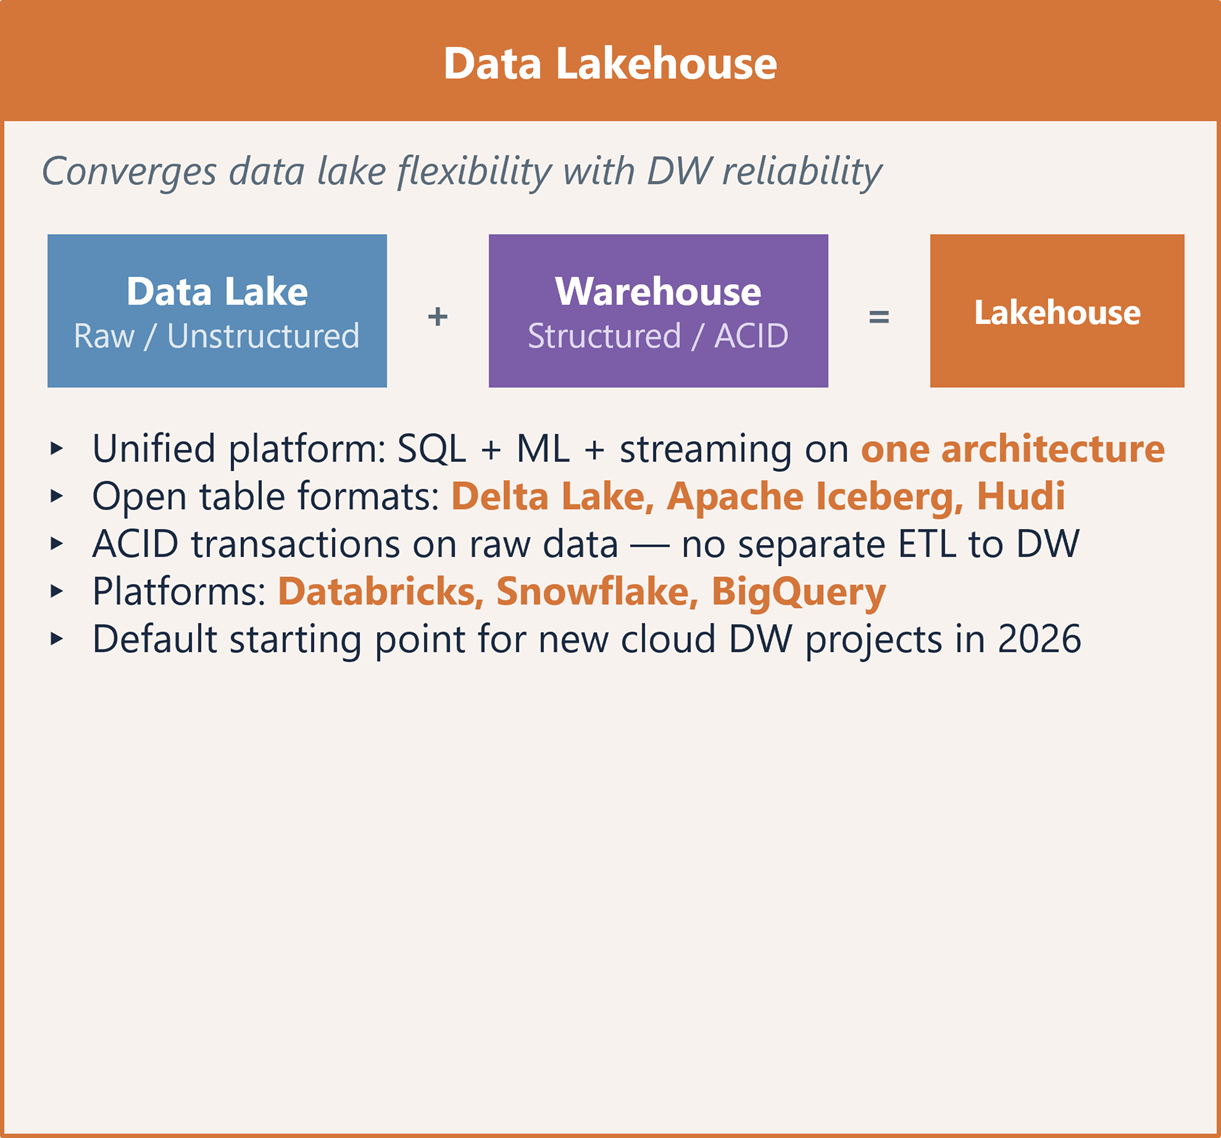
\includegraphics[width=0.85\linewidth]{slike/02/02-28.png}
    \caption{Архитектура језерског складишта (енг. lakehouse): флексибилност језера података (енг. data lake) комбинована са ACID гаранцијама складишта кроз отворене формате табела}
    \label{fig:02-32}
\end{figure}

Две последице ове архитектуре посебно су релевантне за ово потпоглавље. Прво, граница између прихватног (енг. \textbf{\textit{staging}}) и интеграционог слоја из §2.2.4.5 се раствара: сирови и курирани подаци коегзистирају у истом слоју складиштења, разликовани трансакционим гаранцијама формата табеле, а не физичким раздвајањем. Друго, платформа подржава аналитичка оптерећења (SQL упити, BI алати) и оптерећења машинског учења (обука модела, обликовање карактеристика, енг. \textbf{\textit{feature engineering}}) без потребе да се подаци премештају између система, што поједностављује управљање и смањује кашњење између доласка података и њихове накнадне употребе. Databricks је платформа која се најтешње повезује са lakehouse обрасцем, али Snowflake, BigQuery и друга облачна складишта усвојила су lakehouse могућности као део своје основне понуде, и овај образац је ефективно постао подразумевана полазна тачка за нове изворно облачне пројекте складишта (Armbrust et al., 2021).

\paragraph{Изворно облачна складишта}
Cloud-native складишта — Snowflake, Google BigQuery, Amazon Redshift и Microsoft Azure Synapse Analytics — деле архитектонски принцип који их разликује од on-premises складишта: складиштење и рачунарски ресурси су раздвојени, скалирају се независно и наплаћују независно. Складиштење се држи у cloud object storage-у, рачунарски ресурси се по потреби обезбеђују као скуп еластичних virtual warehouses, а упит коме треба више ресурса добија их током трајања упита и ослобађа по завршетку. Овај образац омогућава serverless и pay-per-query оперативне моделе у којима је складиште, из перспективе корисника, једноставно доступно уместо унапред обезбеђено.

Архитектонско раздвајање складиштења од рачунарских ресурса преобликовало је економику складиштења. Цена чувања историјских података пала је на ниво на коме је неиспарљивост — особина коју складиште и постоји да спроведе — постала практично бесплатна, уклањајући један од историјских притисака ка агресивној агрегацији и архивирању података. Еластичност рачунарских ресурса померила је архитектонски баланс ка ELT-у (§2.2.4.7.6), јер сопствени SQL механизам складишта може да апсорбује трансформациона оптерећења која би раније захтевала засебну ETL платформу. Аналитичари индустрије извештавају да је тржиште cloud-native складишта порасло са приближно тридесет осам милијарди америчких долара у 2025. на пројектованих седамдесет милијарди до 2029, што одражава прелазак складишта из специјализоване инфраструктурне компоненте у подразумевану cloud услугу.

\paragraph{Даљи трендови}
Три даља развоја обликују пејзаж складишта крајем 2020-их и заслужују кратак осврт. AI/ML интеграција помера складиште од пасивне платформе за извештавање ка активном аналитичком окружењу у коме се модели обучавају, упити оптимизују, а аномалије детектују компонентама машинског учења уграђеним у само складиште. Интерфејси природног језика, у којима корисници постављају питања на енглеском, а систем генерише SQL, прешли су пут од истраживачких прототипова до комерцијалних производа. Gartner је пројектовао да ће до 2026. већина аналитичких оптерећења у неком облику зависити од AI/ML компоненти.

Data mesh, који је увела Dehghani (2022), образац је управљања и власништва, а не технологија. Он предлаже да одговорност за аналитичке производе података (енг. \textbf{\textit{data products}}) буде децентрализована на пословне домене који податке производе — продаја поседује свој производ података, финансије поседују свој — уз федеративни оквир управљања који обезбеђује интероперабилност. Овај образац је одговор на ограничења скалирања централних тимова за складишта у великим организацијама и није замена за архитектонске обрасце овог потпоглавља; он је питање ко поседује и управља складиштем, а не шта складиште јесте.

\textbf{\textit{Аналитика токова података}} (енг. \textit{streaming analytics}), подржана платформама као што су Apache Kafka и њиховим облачним еквивалентима (Amazon Kinesis, Google Pub/Sub), смањује кашњење између доласка података и аналитичке доступности са сати или дана, колико траје типичан пакетни прозор традиционалног складишта, на секунде. Овај образац је важан за случајеве употребе као што су детекција превара, оперативно праћење и персонализација у реалном времену, у којима вредност одговора брзо опада с временом. Архитектонска интеграција токова података са складиштем остаје активно поље пројектовања, са обрасцима као што су lambda и kappa архитектуре, материјализовани погледи над токовима (енг. \textbf{\textit{materialized streaming views}}) и инкрементална материјализација (енг. \textbf{\textit{incremental materialization}}) преко алата као што је dbt, који нуде различите компромисе између латенције и доследности.

Ови развоји не поништавају архитектонске темеље постављене у §§2.2.3 и 2.2.4. Складиште остаје тематски оријентисано, интегрисано, неиспарљиво и временски варијантно; димензионо моделовање остаје доминантан образац за слој окренут кориснику; ETL или ELT остаје интеграциони механизам. Оно што се променило јесу имплементациона технологија, модел распоређивања и границе између складишта и суседних платформи — а оно што је остало јесте архитектонско расуђивање које стоји у основи улоге складишта као подршке управљачким одлукама.

\subsection{Подршка извештавању}
Одељци 2.1.1–2.1.10 увели су четири технике корисничког слоја (енг. \textbf{\textit{front end}}) — визуализацију (§§2.1.1–2.1.6), израду контролних табли (§2.1.9), приповедање помоћу података (§2.1.7) и пивот табелу — без прецизирања на чему су оне засноване. Ово потпоглавље је обезбедило недостајући позадински слој (енг. \textbf{\textit{back end}}). Завршни одељак прати свако архитектонско својство складишта до одговарајуће способности корисничког слоја, чини те зависности експлицитним и припрема читаоца да у сваком наредном BI артефакту на који наиђе препозна које својство складишта обавља тај посао.

\subsubsection{Од својстава складишта до аналитичких способности}
\textbf{\textit{Усаглашене димензије}} (енг. \textit{conformed dimensions}) омогућавају доследне контролне табле. Контролна табла која на једном екрану приказује приход од продаје, маркетиншку потрошњу и тикете корисничке подршке има смисла само ако су та три броја упоредива — рашчлањена по истим временским периодима, истим регионима и истим сегментима купаца. Усаглашене димензије, интеграциони механизам из §2.2.4.3, архитектонско су средство које ово поређење чини могућим: свака табела чињеница придружује се истој DIM\_DATE, истој DIM\_GEOGRAPHY и истој DIM\_CUSTOMER, са атрибутима дефинисаним и управљаним идентично кроз мартове. Контролна табла коју корисник гради у Power BI-ју или Tableau-у ради зато што је складиште испод ње већ обавило посао усаглашавања (енг. \textit{conformance}).

Неиспарљивост и временска варијантност омогућавају приповедање са историјском дубином. Наратив који објашњава како је пословање стигло у свој тренутни положај захтева податке о сваком претходном положају — кварталне путање прихода, поређења из године у годину, кохорте купаца какве су биле у тренутку када је свака кохорта стечена. Образац дописивања без преписивања (енг. \textbf{\textit{append-only}}) из §2.2.3.4 задржава свако стање кроз које је пословање прошло; дисциплина временске варијантности из §2.2.3.5 организује та стања тако да се могу упитивати по датуму. Способност приповедача да покаже „шта се променило” јесте неиспарљивост и временска варијантност складишта учињена видљивом.

Претходно агрегиране коцке омогућавају интерактивне пивот табеле и продубљивање увида (енг. \textbf{\textit{drill-down}}). Пивот табела је аналитичарев инструмент за сечење мера кроз димензије; §2.2.3.7 дао је формални приказ OLAP коцке као њене структуре података. Интерактивна одзивност коју корисник доживљава — превуците димензију у област редова и посматрајте како се унакрсна табела преобликује, проширите хијерархију и гледајте како се месеци отварају унутар године — јесте рад претходно агрегираних вредности и индексираних претрага (енг. \textbf{\textit{lookup}}) коцке, над унапред израчунатим ћелијама, а не над скенирањем табела чињеница.

Тематски оријентисана интеграција омогућава једну верзију истине кроз визуализације. Финансијска контролна табла која извештава о кварталном приходу и продајна контролна табла која извештава о истом приходу морају показати исти број; прича која цитира неку цифру мора се ускладити са контролним таблама које је приказују; пивот табела коју аналитичар гради за ad hoc анализу мора бити сагласна са оба. Тематска оријентација (§2.2.3.2) и интеграција (§2.2.3.3) чине ово поклапање структурним, а не случајним: сваки артефакт црпи из истог усклађеног, интегрисаног и управљаног приказа пословања, а доследност корисничког слоја (енг. \textbf{\textit{front end}}) јесте, на крају, дисциплина интеграције позадинског слоја (енг. \textbf{\textit{back end}}) учињена видљивом на корисниковом екрану.

\section{Литература}
Armbrust, M., Ghodsi, A., Xin, R., \& Zaharia, M. (2021). Lakehouse: A new generation of open platforms that unify data warehousing and advanced analytics. In Proceedings of the 11th Conference on Innovative Data Systems Research (CIDR).

Becker, R. A., \& Cleveland, W. S. (1987). Brushing scatterplots. Technometrics, 29(2), 127–142.

Bostock, M., Ogievetsky, V., \& Heer, J. (2011). D³ data-driven documents. IEEE Transactions on Visualization and Computer Graphics, 17(12), 2301–2309. https://doi.org/10.1109/TVCG.2011.185

Box, G. E. P., Jenkins, G. M., Reinsel, G. C., \& Ljung, G. M. (2015). Time series analysis: Forecasting and control (5th ed.). Wiley.

Cairo, A. (2016). The truthful art: Data, charts, and maps for communication. New Riders.

Card, S. K., Mackinlay, J. D., \& Shneiderman, B. (1999). Readings in information visualization: Using vision to think. Morgan Kaufmann.

Chaudhuri, S., \& Dayal, U. (1997). An overview of data warehousing and OLAP technology. ACM SIGMOD Record, 26(1), 65–74. https://doi.org/10.1145/248603.248616

Chen, H., Chiang, R. H. L., \& Storey, V. C. (2012). Business intelligence and analytics: From big data to big impact. MIS Quarterly, 36(4), 1165–1188.

Cleveland, W. S. (1993). Visualizing data. Hobart Press.

Cleveland, W. S., \& McGill, R. (1984). Graphical perception: Theory, experimentation, and application to the development of graphical methods. Journal of the American Statistical Association, 79(387), 531–554.

Codd, E. F. (1970). A relational model of data for large shared data banks. Communications of the ACM, 13(6), 377–387. https://doi.org/10.1145/362384.362685

Codd, E. F., Codd, S. B., \& Salley, C. T. (1993). Providing OLAP to user-analysts: An IT mandate. Codd \& Associates.

Cressie, N. (1993). Statistics for spatial data. Wiley.

Davenport, T. H., \& Harris, J. G. (2007). Competing on analytics: The new science of winning. Harvard Business School Press.

Dehghani, Z. (2022). Data mesh: Delivering data-driven value at scale. O’Reilly Media.

Eckerson, W. W. (2010). Performance dashboards: Measuring, monitoring, and managing your business (2nd ed.). Wiley.

Few, S. (2006). Information dashboard design: The effective visual communication of data. O’Reilly Media.

Few, S. (2009). Now you see it: Simple visualization techniques for quantitative analysis. Analytics Press.

Few, S. (2012). Show me the numbers: Designing tables and graphs to enlighten (2nd ed.). Analytics Press.

Few, S. (2013). Information dashboard design: Displaying data for at-a-glance monitoring (2nd ed.). Analytics Press.

Gelman, A., \& Hill, J. (2007). Data analysis using regression and multilevel/hierarchical models. Cambridge University Press.

Golfarelli, M., \& Rizzi, S. (2009). Data warehouse design: Modern principles and methodologies. McGraw-Hill.

Härder, T., \& Reuter, A. (1983). Principles of transaction-oriented database recovery. ACM Computing Surveys, 15(4), 287–317. https://doi.org/10.1145/289.291

Hastie, T., Tibshirani, R., \& Friedman, J. (2009). The elements of statistical learning: Data mining, inference, and prediction (2nd ed.). Springer.

Heer, J., \& Shneiderman, B. (2012). Interactive dynamics for visual analysis. Communications of the ACM, 55(4), 45–54. https://doi.org/10.1145/2133806.2133821

Inmon, W. H. (2005). Building the data warehouse (4th ed.). Wiley.

Inmon, W. H., Strauss, D., \& Neushloss, G. (2008). DW 2.0: The architecture for the next generation of data warehousing. Morgan Kaufmann.

James, G., Witten, D., Hastie, T., \& Tibshirani, R. (2021). An introduction to statistical learning (2nd ed.). Springer.

Kaplan, R. S., \& Norton, D. P. (1996). The balanced scorecard: Translating strategy into action. Harvard Business School Press.

Keim, D. A., Andrienko, G., Fekete, J.-D., Görg, C., Kohlhammer, J., \& Melançon, G. (2010). Visual analytics: Definition, process, and challenges. In A. Kerren et al. (Eds.), Information visualization (pp. 154–175). Springer.

Keim, D. A., Mansmann, F., Schneidewind, J., Thomas, J., \& Ziegler, H. (2008). Visual analytics: Scope and challenges. In Visual data mining (pp. 76–90). Springer. https://doi.org/10.1007/978-3-540-71080-6\_6

Kimball, R., Caserta, J., \& Mundy, J. (2008). The data warehouse ETL toolkit: Practical techniques for extracting, cleaning, conforming, and delivering data. Wiley.

Kimball, R., \& Ross, M. (2013). The data warehouse toolkit: The definitive guide to dimensional modeling (3rd ed.). Wiley.

Kimball, R., Ross, M., Thornthwaite, W., Mundy, J., \& Becker, B. (2008). The data warehouse lifecycle toolkit (2nd ed.). Wiley.

Knaflic, C. N. (2015). Storytelling with data: A data visualization guide for business professionals. Wiley.

Knaflic, C. N. (2020). Storytelling with data: Let’s practice! Wiley.

Kosara, R., \& Mackinlay, J. (2013). Storytelling: The next step for visualization. Computer, 46(5), 44–50. https://doi.org/10.1109/MC.2013.36

Linstedt, D., \& Olschimke, M. (2015). Building a scalable data warehouse with Data Vault 2.0. Morgan Kaufmann.

Marr, B. (2016). Big data in practice: How 45 successful companies used big data analytics to deliver extraordinary results. Wiley.

Munzner, T. (2014). Visualization analysis and design. CRC Press.

Newman, M. E. J. (2018). Networks (2nd ed.). Oxford University Press.

Rahm, E., \& Bernstein, P. A. (2001). A survey of approaches to automatic schema matching. The VLDB Journal, 10(4), 334–350. https://doi.org/10.1007/s007780100057

Sarikaya, A., Correll, M., Bartram, L., Tory, M., \& Fisher, D. (2019). What do we talk about when we talk about dashboards? IEEE Transactions on Visualization and Computer Graphics, 25(1), 682–692.

Satyanarayan, A., Moritz, D., Wongsuphasawat, K., \& Heer, J. (2017). Vega-Lite: A grammar of interactive graphics. IEEE Transactions on Visualization and Computer Graphics, 23(1), 341–350.

Segel, E., \& Heer, J. (2010). Narrative visualization: Telling stories with data. IEEE Transactions on Visualization and Computer Graphics, 16(6), 1139–1148. https://doi.org/10.1109/TVCG.2010.179

Sharda, R., Delen, D., \& Turban, E. (2020). Business intelligence, analytics, and data science: A managerial perspective (4th ed.). Pearson.

Sheth, A. P., \& Larson, J. A. (1990). Federated database systems for managing distributed, heterogeneous, and autonomous databases. ACM Computing Surveys, 22(3), 183–236. https://doi.org/10.1145/96602.96604

Shneiderman, B. (1996). The eyes have it: A task by data type taxonomy for information visualizations. In Proceedings of the IEEE Symposium on Visual Languages (pp. 336–343). IEEE.

Slocum, T. A., McMaster, R. B., Kessler, F. C., \& Howard, H. H. (2009). Thematic cartography and geovisualization (3rd ed.). Pearson.

Stevens, S. S. (1946). On the theory of scales of measurement. Science, 103(2684), 677–680.

Tufte, E. R. (1990). Envisioning information. Graphics Press.

Tufte, E. R. (2001). The visual display of quantitative information (2nd ed.). Graphics Press.

Tukey, J. W. (1977). Exploratory data analysis. Addison-Wesley.

Ware, C. (2013). Information visualization: Perception for design (3rd ed.). Morgan Kaufmann.

Wickham, H., \& Grolemund, G. (2017). R for data science. O’Reilly Media.

Wilke, C. O. (2019). Fundamentals of data visualization. O’Reilly Media.

Wilkinson, L. (2005). The grammar of graphics (2nd ed.). Springer.

% Аутоматски генерисано из ОЗП.docx

\chapter{Откривање законитости у подацима}
\label{ch:ozp}
\textbf{Откривање законитости у подацима (ОЗП)} представља процес у коме се откривају законитости у подацима организација са циљем унапређења и/или аутоматизације процеса одлучивања. Под подацима се подразумевају скупови података, најчешће представљени у табеларној форми (редови табеле представљају случајеве, док колоне представљају атрибуте који описују случајеве), који су добијени из база података, складишта података, али и свих других извора преко којих се прикупљају и складиште подаци (текст, логови, фото, видео и аудио записи).

ОЗП обједињује методе, алгоритме и технике из различитих дисциплина (статистика и вероватноћа, математика, машинско учење, базе података, структуре података). Може да се користи у анализи великих података у организацијама — за разлику од класичне статистичке анализе која је обично користила табеле мањих димензија, ОЗП је намењен за анализу већих количина података и уводи низ нових алгоритама који могу да раде са великим обимом података, разноврснијим типовима података, као и учесталијом фреквенцијом генерисања нових података.

\textbf{Законитости} су правила или модели који важе у специфичном контексту, али не морају нужно да важе у свим ситуацијама (нпр. понашање потрошача у Азији и Европи не мора да подлеже истим законитостима). Са друге стране, \textbf{закони} су оне појаве које имају далеко већи опсег дејства и далеко шири контекст (закон понуде и потражње, закон гравитације). Често се за реч законитост, поготово у инжењерским наукама, користи и појам \textit{патерн}, \textit{архетип}, \textit{узор}.

Откривене законитости су изузетно важне за сваку организацију јер јој омогућавају, између осталог:

\begin{itemize}
  \item боље разумевање пословног процеса,
  \item информисаније доношење одлука,
  \item потенцијално претварање законитости у нову вредност, а самим тим и
  \item могућност аутоматизације процеса одлучивања.
\end{itemize}
Информација (управљачки извештај) оставља простор доносиоцу одлука да донесе одлуку, док откривена законитост може да аутоматизује пословни процес, јер садржи, за разлику од информације, управљачку компоненту.

ОЗП не представља замену за класичну статистичку анализу, већ њену допуну. Знања која су потребна за разумевање метода и резултата статистичке анализе остају и даље неопходна. Истовремено, ма колико примамљиво откривање законитости из података звучи, треба бити опрезан, јер неки кандидати за законитости (идентификована правила или међузависности) могу пре да буду окарактерисани као случајност. Зато се сви добијени модели ОЗП обавезно евалуирају, по могућности статистичким тестовима, како би се сазнало да ли је откривена законитост заиста законитост или је производ погрешно постављеног експеримента или лоше изабраног узорка података.

ОЗП користи скуп алгоритама који захтевају одређена знања од корисника:

\begin{itemize}
  \item разумевање предуслова за рад алгоритма (захтевани тип података, дозвољену количину недостајућих података, захтевану припрему података),
  \item разумевање параметара алгоритма и делимично самог алгоритма,
  \item способност тумачења резултата добијених алгоритмом.
\end{itemize}

\subsection{CRISP-DM методологија}
Да би се ефикасно водили пројекти ОЗП постоје разне методологије. Једна од најпознатијих је \textbf{CRISP-DM} (међуиндустријски стандардни процес за откривање законитости у подацима). Састоји се из следећих фаза:

\begin{itemize}
  \item Разумевање пословног проблема,
  \item Разумевање података,
  \item Припрема података,
  \item Моделовање решења,
  \item Евалуација модела,
  \item Примена модела.
\end{itemize}
Методологија CRISP-DM је итеративног карактера са циљем да се дође до система ОЗП који је ефикасан и ефективан.

\subsubsection{Разумевање пословног проблема}
Прва фаза има за циљ да аналитичар добро разуме пословни проблем, да схвати који је циљ који треба да оствари будућим системом ОЗП. У овој фази развојни тим треба од стране доменских експерата да сазна захтеве које систем ОЗП треба да испуни. Ово је фаза у којој би требало да подстакне учење развојног тима, али и доменских експерата који често нису свесни домета које систем ОЗП може да оствари.

У овој фази се дефинишу циљеви и хипотезе истраживања, а такође се описују основни појмови из области у којој се ради анализа.

\subsubsection{Разумевање података}
Фаза у којој се аналитичар упознаје са подацима са којима треба да ради и да према томе одреди који му алгоритми, методе, архитектуре стоје на располагању. У овој фази се добијају сазнања о квалитету, формату и употребљивости података за анализу.

Аналитичар треба да обрати пажњу на:

\begin{itemize}
  \item \textbf{Тип података}:
  \begin{itemize}
    \item \textbf{Категорички} — ненумерички, без могућности успостављања поретка међу категоријама (нпр. за атрибут тип писаљке, категорије могу бити оловка, хемијска, фломастер).
    \item \textbf{Ординални} — категорички подаци у којима међу категоријама може да се успостави одређени поредак (нпр. вруће, топло, свеже, хладно).
    \item \textbf{Нумерички} — поред особина једнаког растојања међу бројевима имају и особину смислене нулте вредности.
  \end{itemize}
  \item \textbf{Смер података}:
  \begin{itemize}
    \item \textbf{Улазни} (познати и као дескриптори) — служе за прављење модела за предвиђање излазних атрибута, или се користе самостално.
    \item \textbf{Излазни} (познати као предиктори) — подаци које је потребно предвидети на основу улазних података.
  \end{itemize}
  \item \textbf{Корелација међу подацима} — мери се најчешће коефицијентом корелације, са вредностима у распону од -1 до 1, где 0 означава одсуство корелације, 1 апсолутну корелисаност, а -1 апсолутно негативну корелисаност. Корелација се испитује између парова улазних атрибута, излазних атрибута, као и улазних и излазних атрибута.
  \item \textbf{Дистрибуција (расподела) података} — колико су подаци учестали за конкретне вредности. Најчешће алгоритми претпостављају нормалну расподелу података (у којој се аритметичка средина најчешће појављује), мада постоје и многе друге могуће расподеле података (нпр. униформа у којој свака вредност може да се појављује са истом учесталошћу), а аналитичар би требало да буде упознат са овим расподелама.
  \item \textbf{Недостајуће вредности} — треба одлучити да ли редове са недостајућим подацима избацити из анализе или применити неку технику попуњавања (аритметичка средина за нумеричке, модус за категоричке).
  \item \textbf{Екстремне вредности} — аналитичар треба да донесе одлуку да ли да задржи аномаличне вредности у подацима или да их избаци и прогласи екстремима.
\end{itemize}
Аналитичар у фази разумевања података користи графике, али може да користи и алгоритме машинског учења како би стекао увиде у квалитет података и прелиминарну могућност аналитичке обраде истих.

\subsubsection{Припрема података}
Основни задатак припреме података јесте да се подаци за анализу сместе у табеларни облик (где колоне представљају атрибуте, а редови случајеве) или неки други погодан облик над којим је могуће спровести алгоритме ОЗП и открити законитости. Активност припреме података може да се схвати као функција која податке из неструктурираног облика претвара у структуриран облик за алгоритме, тј. облик неопходан за успешан рад алгоритама.

Сваки алгоритам захтева податке у одређеном формату и поседује претпоставке са каквим особинама података треба да ради. Алгоритми, осим ако то софтверски није подржано, не проверавају да ли је посао припреме података добро урађен — управо је посао аналитичара да податке доведе у исправан облик. Ова фаза, заједно са разумевањем података и пословног проблема, одузима знатан део времена у пројекту развоја система ОЗП.

Различито припремљени подаци могу да произведу различите излазе из модела, тако да треба наћи праву меру између степена припреме података (чиме се најчешће губи одређени квалитет података) и задржаног квалитета података који гарантују проналажење одређених законитости.

Технике за припрему података се грубо могу поделити у две категорије:

\begin{itemize}
  \item \textbf{Рад са редовима (случајевима)}:
  \begin{itemize}
    \item Селекција — креирање упита који извлачи одређени подскуп занимљив за анализу,
    \item Узорковање — узимање узорка из скупа података,
    \item Балансирање излазног атрибута — кад алгоритам тражи једнак или сличан број категорија по излазном атрибуту,
    \item Агрегирање — рачунање одређене сумарне статистике као што је нпр. центроид код алгоритма К-средина.
  \end{itemize}
  \item \textbf{Рад са колонама (атрибутима)}:
  \begin{itemize}
    \item Дефинисање типа и смера атрибута (могуће је исте податке посматрати или као категоричке или као ординалне или као нумеричке. Нпр. оцена на испиту може бити све три категорије, при чему различити алгоритми захтевају различити тип података),
    \item Филтрирање — избацивање нежељених атрибута,
    \item Извођење нових атрибута — на основу постојећих атрибута. Овај процес је изузетно значајан јер може да произведе атрибуте на основу којих алгоритам може да открије корисније законитости. Код дефинисања ових атрибута помоћ експерата је од пресудног значаја.
    \item Дискретизација — трансформисање нумеричких података у ординалне, тј. у распоне података или корпе. Овај процес као и извођење нових атрибута може помоћи у откривању значајнијих законитости.
  \end{itemize}
\end{itemize}

\subsubsection{Моделовање решења}
Када су схваћени пословни проблеми и подаци, и када су подаци припремљени, могуће је покренути алгоритме ОЗП. Процес моделовања решења представља централни део у изради пројекта ОЗП и најчешће се на њега мисли када се каже ОЗП. Ипак, овај део узима најмањи део времена у једном пројекту. Учешће људског фактора односи се на избор једног или више алгоритама и подешавање параметара изабраних алгоритама. У оквиру ове фазе битно је поставити и експеримент (нпр. унакрсна валидација, раздвајање података на скуп података за учење и проверу) за евалуацију модела ОЗП и развити такав модел који постиже математички одговарајућа мерила квалитета. Обично се овај процес евалуације означава као \textbf{верификација} — провера да ли машински научен модел ОЗП математички задовољава прагове квалитета.

\subsubsection{Евалуација система ОЗП}
Евалуација решења представља активност која треба да испита валидност (употребљивост, исправност) добијеног решења са стране корисника будућег система ОЗП. Математичка евалуација развијеног модела је део фазе моделовање решења. У овој фази се ради \textbf{валидација система ОЗП} — тј. да ли систем ОЗП може да унапреди у реалној пракси процес одлучивања и тиме оствари циљеве који су постављени у фази разумевања пословног проблема.

\subsubsection{Примена модела}
У процесу примене решења може да се сазна колико је систем ОЗП заиста употребљив. У овој фази се решење примењује над реалним окружењем, с тим да и даље постоји могућност да решење није у потпуности задовољавајуће, те се током рада адаптира и модификује. Током реалне примене система ОЗП константно се прате перформансе система, а систем се са времена на време унапређује, модификује или одбацује.

\subsection{Задаци ОЗП}
Задаци ОЗП представљају области примена система ОЗП. Сваки систем ОЗП може да има за циљ испуњавање једног или више задатака:

\begin{itemize}
  \item \textbf{Редукција} — свођење података на димензије које могу да се анализирају на ефикасан начин.
  \item \textbf{Регресија} — учење модела ОЗП који моделује везу између улазних атрибута и излазног атрибута који је нумеричког типа.
  \item \textbf{Класификација} — учење модела ОЗП који моделује везу између улазних атрибута и излазног атрибута који је категоричког или ординалног типа.
  \item \textbf{Кластеровање} — груписање случајева према сличности у одређени број група које нису унапред познате. Број група може да се одреди унапред, али и може да се врши претрага оптималног броја група, тј. кластера.
  \item \textbf{Асоцијативна и класификациона правила} — откривање ако-тада правила у структурама табелама и трансакцијама.
  \item \textbf{Предвиђање} — решавање свих претходних задатака у неком будућем временском периоду, нпр. за наредни дан, за наредну недељу, месец, годину.
\end{itemize}
Број задатака овим списком није исцрпљен, могући су разни хибридни задаци који комбинују наведене задатке са просторном и временском димензијом.

\subsubsection{Редукција/Оптимизација избора атрибута и случајева}
Основни циљ редукције је смањивање димензије проблема на онај облик који је повољан за анализу и који успоставља компромис између брзине решавања проблема и квалитета података за анализу. Може бити:

\begin{itemize}
  \item \textbf{Редукција атрибута} или селекција атрибута је оптимизациони проблем чији је циљ изабрати онај скуп атрибута који налази оптималан однос између жељених мера квалитета и количине неопходних атрибута. У данашње време процеси избора оптималног скупа атрибута су постали изузетно успешни и омогућавају да се простор оригиналних атрибута знатно смањи или замени новим, тзв. „скривеним“ слојем атрибута који одлично репрезентује оригиналне атрибуте.
  \item \textbf{Редукција случајева (редова)} је процес узорковања података, са циљем да се нађе узорак који веродостојно репрезентује претпостављену популацију. Овај задатак је исто изузетно сложен јер некад и не постоји довољно редова за анализу, па је потребно генерисати вештачки нове редове не би ли се дошло до одређеног броја случајева.
\end{itemize}

\subsubsection{Процена (регресија)}
Процена је задатак који има за циљ да открије модел који постоји између улазних атрибута и излазног атрибута нумеричког типа. Решава се коришћењем линеарних модела (линеарна регресија) или сложенијих алгоритама (вештачке неуронске мреже) које представљају универзалне апроксиматоре. Линеарни модели су по правилу апроксимација неког реалног нелинеарног модела, али се широко користе јер су једноставнији и разумљивији.

\subsubsection{Класификација}
Класификациони алгоритми уче моделе који праве функцију између улазних атрибута са излазним категоричким атрибутом. Излазни категорички атрибут је познат као класни атрибут. Задатак класификације је да открије законитост по којој се одређени објекат (ред у табели) сврстава у одређену класу.

Ако излазни атрибут има само две категорије (нпр. да/не) онда се ради о бинарној класификацији. У осталим случајевима ради се о вишеструкој класификацији.

Ако је потребно предвидети више излазних атрибута истовремено тада се користе алгоритми класификације за више излазних атрибута (више етикета).

\subsubsection{Кластеровање}
Док класификација служи да открије модел по коме се објекти распоређују у унапред познате класе (надгледано учење), кластеровање треба да пронађе законитост на основу које се објекти групишу у класе које нису познате на почетку процеса. Кластер је класа која није позната на почетку процеса тражења законитости, већ треба да се открије самим процесом кластеровања, да се протумачи и верификује. Због недостатка излазног атрибута, као у случају класификације, спада у класу алгоритама ненадгледаног учења. Ненадгледано учење значи да се у подацима не тражи повезаност између улазних атрибута и неког излазног атрибута, већ се у недостатку тог атрибута, заправо случајеви групишу по сличности.

Кластеровање је процес откривања група таквих да су објекти унутар кластера међусобно слични, а да су притом прилично различити од објеката других кластера. (Ово је дефиниција која је карактеристична за алгоритам К-средина, док други алгоритми кластеровања могу да претпостављају и различите дефиниције кластера.)

Кластеровање се спроводи из следећих разлога:

\begin{itemize}
  \item када нису унапред познате класе за разврставање објеката,
  \item пружа више информација о природи груписања објеката, тј. припадност кластера може даље да се користи као ново сазнање у процесу ОЗП. То чак може да се тумачи као нека „скривена“ особина.
  \item омогућава да се редукује број случајева који се анализирају тако што се уместо случајева који се налазе у кластеру узима само њихов представник. Тако је могуће заправо процес редукције случајева урадити уз помоћ алгоритама кластеровања при чему је потребно одредити број кластера који се жели имати. Представници ових кластера могу после да постану редуковани случајеви,
  \item омогућава организацијама да боље разумеју специфичности својих корисника.
\end{itemize}
Након развоја модела кластеровања, сваком случају може да се додели одређени излазни атрибут — припадност кластеру — чиме се отвара пут за коришћење техника класификације које могу да помогну да се открију законитости по којој су објекти кластеровани.

\subsubsection{Асоцијативна и класификациона правила}
Код класичне статистичке анализе аналитичар или ДО сами претпостављају правило (тј. хипотезу), док код ОЗП аналитичар задаје само параметре претраге за одређеним правилима, а алгоритам самостално открива законитости.

Асоцијативна правила су облика \textbf{АКО узрок ТАДА последица} и према томе су лако схватљива и применљива за моделовање знања. Битна су за разумевање и унапређење пословног процеса — омогућавају да се уоче неке законитости које се иначе тешко уочавају.

Класични проблеми који се решавају асоцијативним правилима су:

\begin{itemize}
  \item \textbf{Анализа потрошачке корпе} која може да одговори на питања који производи се купују заједно, или да ли куповина одређеног производа утиче на куповину другог производа.
  \item \textbf{Системи препоруке} — на основу куповине одређених производа препоручити потенцијално занимљив производ кориснику на основу сличних образаца куповине других корисника или особина које сам корисник поседује.
\end{itemize}

\subsubsection{Предвиђање}
Сваки претходно објашњени задатак истовремено може да служи и за предвиђање, поред алгоритама временских серија који природно у себи укључују и временску димензију. Постоје алгоритми за редукцију, процену, класификацију, кластеровање и откривање асоцијативних правила са подацима са временском димензијом али је могуће и инжењерингом података развити моделе за предвиђање будућих стања посматраног система.

\section{Алгоритми за откривање законитости у подацима}
У наставку ће бити представљено неколико алгоритама за откривање законитости у подацима, груписаних по следећим типовима:

\begin{itemize}
  \item \textbf{Алгоритми за компресију и откривање скривених фактора} — служе да се нађе компресована репрезентација оригиналних података таква да смањи величину улазног простора што више, а да задржи квалитет декомпресије у оригинални простор података.
  \item \textbf{Стабла одлучивања} — решавају задатак класификације и регресије, уче модел у облику дрвета одлучивања.
  \item \textbf{Асоцијативна и класификациона правила} — откривају правила облика Ако-Тада сходно постављеним праговима подршке и поверења (ови термини ће бити објашњени у наставку).
  \item \textbf{Алгоритми за кластеровање} — откривају груписања у подацима.
  \item \textbf{Регресиони алгоритми} — уче модел зависности између улазних и излазног податка нумеричког типа.
  \item \textbf{Вештачке неуронске мреже} — представљају универзални апроксиматор (може до перфекције да се научи над скупом података за учење) за решавање задатака класификације и процене.
\end{itemize}

\subsection{Редукција}
Постоји мноштво алгоритама који се користе за редукцију. Овде ћемо се концентрисати на редукцију атрибута, јер се алгоритми који се овим баве користе стандардно у процесима ОЗП.

Неки од најпознатијих алгоритама редукције који врше компресију улазних података у тзв. скривени (латентни) слој су:

\begin{itemize}
  \item \textbf{Анализа главних компоненти} — оригиналан скуп атрибута трансформише у скуп главних компоненти таквих да када се оригинални подаци пројектују на главне компоненте, међу њима не постоји зависност (корелација је једнака 0), док је варијабилитет појачан на првим компонентама. Открива се онолико компоненти колико има почетних атрибута, али се најчешће користило само 20\% компоненти да опише 80\% варијансе која се налази у подацима. У данашње време модерни алгоритми могу у неким случајевима да открију 1\% компоненти које описују 99\% варијансе која постоји у подацима.
  \item \textbf{Факторска анализа} — слично анализи главних компоненти ради екстракцију скривених фактора, али те факторе тражи над заједничком варијансом, а не укупном као код анализе главних компоненти. Ова наизглед мала разлика је суштинска, јер скривени фактори над заједничком варијансом омогућавају интерпретабилност ових фактора. У друштвеним наукама се преферира факторска анализа над анализом главних компонената чије откривене компоненте не морају нужно да имају значење у реалности.
\end{itemize}

\subsection{Асоцијативна и класификациона правила}
Асоцијативна правила представљају један од основних облика законитости какве се откривају код ОЗП — облик АКО-ТАДА. Алгоритми ОЗП откривају законитости у облику АКО (категорија, или конјункција категорија) ТАДА (категорија или конјункција категорија). Њихов циљ је да нађу скуп правила који, за задате параметре, откривају све постојеће АКО-ТАДА релације.

Асоцијативна правила представљају једну од првих техника које су се користиле код ОЗП. У наставку ће бити представљен један од најпознатијих алгоритама за откривање асоцијативних правила, Apriori.

\subsubsection{Разумевање података}
Алгоритам ради искључиво са категоричким (ненумеричким) подацима, тако да је корисно све податке припремити тако да буду ненумеричког типа. Уколико у скупу података постоје нумерички подаци, потребно је те податке претворити у категорички тип података.

\subsubsection{Трансформација података}
У случају да су атрибути нумеричког типа, потребно је дискретизовати податке, тј. нумеричке податке претворити у дискретне вредности. Неке од основних техника:

\begin{itemize}
  \item \textbf{Аритметичка средина ± n × стандардна девијација} — могуће је направити 3 интервала, 5 интервала и слично. Тако нпр. 3 интервала овом методом имаће следеће границе: (-∞, средина − девијација], (средина − девијација, средина + девијација], (средина + девијација, +∞).
  \item \textbf{Једнака фреквенција} — могуће је направити предефинисани број категорија тако да у сваком интервалу буде подједнак број елемената.
  \item \textbf{Кориснички дефинисани интервали} — границе одређује експерт на основу доменског знања.
\end{itemize}
\textbf{Пример:} атрибут потрошња минута разговора дневно за седам корисника, са вредностима: 50, 60, 65, 70, 80, 120 и 150. Циљ је дискретизација у три категорије: ниска, средња и висока.

\begin{itemize}
  \item \textbf{Метод средине и девијације:} аритметичка средина ≈ 85, стандардна девијација ≈ 35. Границе: (−∞, 50], (50, 120], (120, +∞). Вредност 50 → ниска; 60, 65, 70, 80, 120 → средња; 150 → висока.
  \item \textbf{Метод једнаке фреквенције:} сортирати растуће и поделити на три групе. Вредности 50 и 60 → ниска; 65 и 70 → средња; 80, 120 и 150 → висока.
  \item \textbf{Кориснички дефинисани интервали:} нпр. ≤ 60 ниска; (60, 100] средња; > 100 висока. Вредности 50 и 60 → ниска; 65, 70, 80 → средња; 120 и 150 → висока.
\end{itemize}

\subsubsection{Моделовање решења}
Да би алгоритам Apriori могао да почне своју претрагу потребно је дефинисати два параметра:

\begin{itemize}
  \item \textbf{Подршка} представља вероватноћу појављивања одређене категорије у подацима. Подршка може да се односи како на АКО део правила, тако на ТАДА део правила, али и на цело АКО-ТАДА правило. Говори о томе колико је правило или део правила заступљен у подацима. Обично се користи подршка АКО дела правила као почетни параметар, али у зависности од софтвера који се користи то може бити и другачије.
  \item \textbf{Поверење} представља условну вероватноћу АКО-ТАДА правила, тј. вероватноћу појављивања одређеног ТАДА дела правила у подскупу података АКО дела правила.
\end{itemize}
\textbf{Пример 1.} Анализира се 1000 трансакција куповина производа. Подршка куповине чоколаде $P(\textrm{чоколада})$ је 5\%, што значи да се у 50 куповина појављивала чоколада. Поверење куповине негазираног сока у куповинама чоколаде $P(\textrm{негазирани сок} \mid \textrm{чоколада})$ је 60\%, што значи да се у 50 куповина чоколаде негазирани сок појавио 30 пута.

Кораци алгоритма:

\begin{itemize}
  \item Претражити над свим категоријама (подскуповима) (почевши од скупова са једним елементом) инкрементално увећавајући скуп за по један елемент док год су подскупови заступљени задатом подршком. Скупови података (категорија) који задовољавају задату подршку се називају и фреквентни (учестали) скупови података.
  \item Унутар свих учесталих скупова података проверити да ли је између подскупова задовољено задато поверење. Сачувати она правила над којима је задовољено поверење.
\end{itemize}
Сам процес је рачунски врло захтеван јер се претражују све могуће комбинације подскупова података. Убрзавање поступка омогућава следеће правило:

\textit{Подршка било ког учесталог подскупа података мора имати подршку мању или једнаку учесталом скупу у коме је садржан подскуп.}

Ово омогућава да се простор претраге смањи јер нема сврхе претраживати оне подскупове чији скупови нису имали одговарајућу подршку.

\textbf{Пример 2.} Посматрамо 1000 трансакција куповина у супермаркету. Параметри: подршка = 0.3, поверење = 0.6.

\begin{itemize}
  \item У првој итерацији претражују се сви скупови са једним производом. Откривене подршке: $P(\textrm{пециво}) = 30\%$, $P(\textrm{млечни производи}) = 25\%$, $P(\textrm{сок}) = 33\%$.
  \item У следећој итерацији се претражују подскупови са два производа који имају степен подршке најмање 30\%. Види се да $P(\textrm{пециво, млечни производи}) = 18\%$, $P(\textrm{пециво, сок}) = 20\%$, $P(\textrm{млечни производи, сок}) = 15\%$ не могу да остваре жељени ниво подршке те само правило (пециво, сок) може имати тражену подршку у даљим итерацијама.
  \item Проверава се поверење: $P(\textrm{пециво} \mid \textrm{сок}) = 55\%$, $P(\textrm{сок} \mid \textrm{пециво}) = 65\%$. Откривена је законитост $P(\textrm{сок} \mid \textrm{пециво})$ која говори да се од свих куповина пецива сок купује у 65\% случајева. $P(\textrm{АКО пециво ТАДА сок}) = 65\%$.
\end{itemize}

\subsubsection{Евалуација модела}
Код асоцијативних правила је изузетно битно проверити ваљаност датог правила процесом верификације (мерама квалитета) и валидације (потврдом од стране експерата). Да би се проценио квалитет користе се три основне мере:

\textbf{Подршка} (Support) — мери колико се често правило појављује у скупу података.

\[
\textrm{подршка}(X \Rightarrow Y)=\frac{\vert \{t \in T : X \cup Y \subseteq t\}\vert }{\vert T\vert }
\]

где је T скуп свих трансакција, t једна трансакција, \(X \cup Y\) скуп ставки у правилу. Узима вредности између 0 и 1. Већа вредност значи да је правило чешће у подацима. Правила са веома малом подршком се често одбацују.

\textbf{Поверење} (Confidence) — мери колико често се ТАДА део правила Y појављује у трансакцијама које већ садрже АКО део X.

\[
\textrm{поверење}(X \Rightarrow Y)=\frac{\textrm{подршка}(X \cup Y)}{\textrm{подршка}(X)}
\]

Узима вредности између 0 и 1. Високо поверење значи да правило има добру предиктивну моћ. Међутим, високо поверење не мора нужно значити и јаку повезаност између X и Y.

\textbf{Надмашивач} (Lift) — мери колико је појава X и Y заједно већа (или мања) од очекиване вредности у случају њихове независности.

\[
\textrm{подизач}(X \Rightarrow Y)=\frac{\textrm{поверење}(X \Rightarrow Y)}{\textrm{подршка}(Y)}=\frac{\textrm{подршка}(X \cup Y)}{\textrm{подршка}(X) \cdot \textrm{подршка}(Y)}
\]

\begin{itemize}
  \item Надмашивач = 1 → не постоји веза између АКО и ТАДА дела правила.
  \item Надмашивач > 1 → постоји позитивна повезаност (АКО део повећава вероватноћу ТАДА дела).
  \item Надмашивач < 1 → АКО део правила утиче негативно на ТАДА део.
\end{itemize}
\textbf{Пример:} имамо 100 трансакција. У 30 се појављује X, у 40 се појављује Y, у 20 се заједно појављују X и Y.

\begin{itemize}
  \item Подршка = $20 / 100 = 0.20$
  \item Поверење = $20 / 30 \approx 0.67$
  \item Надмашивач = $0.67 / 0.40 \approx 1.67$
\end{itemize}
Резултати показују да се правило појављује у 20\% свих трансакција, у 67\% случајева када се појави X појављује и Y, а повезаност је позитивна и значајна (надмашивач > 1).

\subsubsection{Примена модела}
Асоцијативна правила могу да се користе у реалним ситуацијама као системи препоруке — да се корисницима јављају препоруке о евентуално занимљивим производима на основу до сада прегледаних. Користе се и за прављење база правила које се покрећу у реалном времену. Седамдесетих година прошлог века су експертски дефинисана асоцијативна правила коришћена за развој експертних система, а данас се често користе у системима извештавања у реалном времену (нпр. препоруке возачима за безбедну вожњу на аутопуту).

\subsection{Алгоритми за кластеровање}
Кластер алгоритми служе да случајеве у скупу података групишу у подскупове који су хомогенији од почетног скупа. Постоје различите фамилије алгоритама кластеровања:

\begin{itemize}
  \item \textbf{Засновани на представницима} — модел кластера се представља преко једног представника који је најчешће централни објекат кластера (нпр. аритметичка средина - центроид, или најцентралнији реални случај у кластеру - медоид). Најпознатији представник је алгоритам К-средина (k-means).
  \item \textbf{Хијерархијски} — сличности међу кластерима представљају у угњежденој хијерархијској структури тако да кластер на врху стабла садржи цео скуп података, а најнижи чворови представљају саме елементе скупа. Најпознатије врсте су агломеративни (полазе од претпоставке да су сви елементи посебан кластер и итеративно их уједињују у један кластер) и дивизиони (полазе од претпоставке да су сви елементи у истом кластеру и итеративно их деле до појединачних случајева). И код дивизионог и хијерархијског кластеровања, стабло представља процес угњеждавања/рашчлањивања објеката од целог скупа до појединих случајева или обрнуто.
  \item \textbf{Засновани на густини} — кластер се дефинише као подскуп који у одређеној околини има довољан број елемената. Алгоритам повезује све елементе скупа који имају сличну густину у један кластер.
\end{itemize}
Наведене три групе кластера имају сасвим другачији поглед на оно што јесу кластери, те се у реалној пракси често комбинују или користи она фамилија алгоритама која одговара проблему који се решава.

Сви кластер алгоритми откривају законитости груписања. Законитост код кластер алгоритма представља правило по коме се случај додељује кластеру.

Битно је напоменути да не постоји најбоље кластеровање, већ је најприхватљивији кластер модел онај који за доносиоца одлука има највише смисла и на основу кога могу да се доносе квалитетне одлуке.

\subsection{Алгоритам К-средина}

\subsubsection{Разумевање пословног проблема}
Једна од најчешћих примена кластеровања је сегментација корисника, како би се боље сазнале специфичне особине појединих група. Различите организације имају различите стратегије — неке праве један исти производ за све кориснике, а неке желе да омогуће да сваки клијент има себи својствен производ. И један и други сценарио делују прилично утопистички те се већина организација одлучује за управљање одређеног броја сегмената преко којих даље може да се боље прилагоди својим корисницима, кроз посебне пакете услуга и производа. Кластеровање може математички да помогне да се открију законитости груписања корисника.

Кластеровање је вишеатрибутивно груписање објеката (за разлику од сортирања које не може истовремено да сортира по више атрибута, већ се то ради лексикографски, тј. по одређеном редоследу).

Кластеровање је вероватно најзаступљенија фамилија алгоритама ОЗП, јер поред свог задатка ОЗП помаже и решавању других задатака ОЗП. Нпр. кластеровање се широко користи и у анализи слика (рендгенски снимци, сателитски снимци) ради идентификације занимљивих сегмената и откривање законитости таквих група.

\subsubsection{Разумевање података}
Подразумевано, алгоритам К-средина ради са нумеричким подацима. Мера сличности коју користи је еуклидско одстојање (корен збира квадратних одстојања) да би се одредило одстојање између сваког случаја и представника група. Због особине да користи еуклидско одстојање, алгоритам је добар за проналажење кластера сферног облика, тако да неће радити ефикасно са кластеровањем нпр. слика у којима треба да се препозна несферичан облик. (Ипак, различите имплементације омогућавају мерење сличности и помоћу других мера сличности, те проблем налажења несферичних облика може да се предупреди.)

Алгоритам је изузетно осетљив на:

\begin{itemize}
  \item \textbf{Атрибуте различитих величина скала} — ако је један атрибут изражен у $[10^3, 10^4]$, а други у децималним $[10^{-1}, 10^{-2}]$, тада други атрибут неће уопште утицати на мерење сличности. Због овога је неопходно користити нормализацију, скалирање атрибута пре примене самог алгоритма.
  \item \textbf{Аномаличне (екстремне) вредности} — вредности које значајно одступају од осталих елемената скупа могу значајно да утичу на перформансе алгоритма к-средина. Нпр. ако би се као почетни представник (центроид) једног од к кластера изабрао случај који је аномаличан, могла би да се деси ситуација да тај кластер не би успео да привуче ниједан други елемент, чиме би такав кластер сам по себи остао бесмислен. Овај проблем се решава или прелиминарном редукцијом скупа података уклањањем свих аномаличних случајева, или „паметним“ одабиром почетних к представника.
\end{itemize}

\subsubsection{Трансформација података}
Алгоритам захтева да су сви подаци нумеричког типа. Ако постоји атрибут ненумеричког типа, могуће је извршити трансформацију категоричког у нумерички тип. То се најчешће ради бинарним кодирањем у којем свака категорија добије један бинарни запис.

Да би се сви нумерички подаци довели у исти распон, могуће је користити методе нормализације, скалирања:

\begin{itemize}
  \item Скалирање у односу на збир вредности одређеног атрибута (збир скалираних вредности ће бити 1).
  \item Скалирање у односу на највећу вредност одређеног атрибута (једна вредност ће бити 1, остале представљају процентуални удео).
  \item Скалирање у односу на аритметичку средину и стандардну девијацију (од почетне вредности се одузима аритметичка средина, разлика се дели стандардном девијацијом). Ова метода је врло корисна и за идентификацију аномаличних вредности једног атрибута — оне најчешће одступају две или више стандардних девијација у односу на аритметичку средину.
\end{itemize}

\subsubsection{Моделовање решења}
Алгоритам поседује параметар \textit{к} (број кластера) који треба да се зада пре него што алгоритам почне са радом. Пошто најчешће није очигледно колико кластера постоји у подацима (знамо да се тај број креће од 1 до укупног броја случајева у скупу података), често се алгоритам покреће више пута са различитим вредностима \textit{к} уз активно учешће доменског експерта. Док алгоритам к-средина може математички да одреди оптималан број кластера, доменски експерт је тај који одлучује да ли је решење прихватљиво, да ли су коришћени одговарајући атрибути за кластеровање, и слично.

Кораци алгоритма:

\begin{enumerate}
  \item Из скупа података насумично изабрати \textit{к} случајева и прогласити их центроидима (представницима).
  \item Све остале елементе скупа доделити најближим представницима тако што се сви случајеви доделе представнику од кога су најмање удаљени.
  \item Прерачунати к центроида као средње вредности случајева који су додељени одговарајућим кластерима.
  \item Понављати кораке 2 и 3 до конвергенције. (Ово значи да нема више прелажења случајева међу кластерима или да константно исти случајеви остају у истим кластерима.)
\end{enumerate}
Почетна фаза случајне иницијализације центроида је осетљива, те се често алгоритам покреће више пута за дефинисано \textit{к} да би се избегла ситуација да један од представника буде аномалија.

\subsubsection{Евалуација модела}
За верификацију модела кластеровања постоје бројне мере квалитета кластера.

\textbf{Индекс силуете/сенке} (Silhouette index) је једна од најпопуларнијих мера квалитета:

\[
s_{i}=\frac{b_{i}-w_{i}}{\max(b_{i},w_{i})}
\]

где је:

\begin{itemize}
  \item $b(i)$ (between, између) — просечна удаљеност случајева посматраног кластера од случајева у најближем суседном кластеру,
  \item $w(i)$ (within, унутар) — просечна међусобна удаљеност случајева унутар припадајућег кластера.
\end{itemize}
Индекс сенке проверава да ли је одређени елемент сличнији елементима унутар свог кластера или елементима најближег суседног кластера. Узима вредности у интервалу од -1 до 1, где 1 значи апсолутну припадност припадајућем кластеру, док -1 означава неприпадност. Срачунава се за сваки случај и на крају се рачуна средња вредност свих индекса сенки и тај сумарни број означава квалитет модела кластеровања. Пожељно је да ова вредност буде што ближа јединици. Вредности 0,5 и веће означавају да сви елементи у просеку више припадају свом кластеру него најближем суседном кластеру. У реалним применама вредности изнад 0,4 су исто прихватљиве.

\textbf{Инерција} представља збир квадрата свих унутар-кластерских растојања и она представља меру компактности појединих кластера. Дефинише се као збир квадрата растојања свих објеката од представника (центроида) кластера којем припадају. Нижа вредност значи да су објекти ближи својим центрима, односно да су кластери компактнији и хомогенији.

Важно је напоменути да се вредност инерције готово увек смањује са повећањем броја кластера. Због тога се инерција не може посматрати изолована, већ се најчешће користи у комбинацији са методама за избор броја кластера.

\textbf{Лакат метода} представља интуитиван приступ за одређивање оптималног броја кластера. Заснива се на анализи промене вредности инерције у зависности од броја кластера. Алгоритам кластеровања се покреће више пута за различите вредности броја кластера (нпр. од 2 до 10), при чему се за сваку вредност израчунава инерција. У почетку, повећање броја кластера доводи до значајног смањења инерције. Након одређеног броја кластера, даљи раст доноси све мања побољшања. Тачка на графику где долази до нагле промене у брзини опадања инерције подсећа на облик лакта, по чему је метода и добила име. Број кластера који одговара тој тачки сматра се оптималним.

\textbf{Валидација} је процес у коме корисник треба да потврди да пронађени кластери одговарају траженим сегментима и да на основу њих може да ефикасније одлучује. Корисник при процесу валидације прегледа центроиде и покушава да их протумачи. Ако су центроиди разумљиви и корисни доносиоцу одлука, кластер модел може да се прогласи прихватљивим. Наравно да корисника система занима и да ли је кластер модел математички прихватљив, али то се подразумева да је тако. Тек математички исправан кластер модел се пружа ДО на разматрање. ДО затим сваком кластеру може да додели одређене стратегије, тактике, производе, услуге, и/или да спроводи управљачке акције.

\subsubsection{Примена модела}
Модел к-средина се заправо састоји од \textit{к} центроида, тј. агрегираних (упросечених) представника својих кластера. Они представљају законитости модела кластеровања, тј. законитост по којој се случајеви расподељују у групе. У фази примене то значи да центроиди одређују над подацима над којима модел није учио који случајеве додељује ком кластеру.

Алгоритам К-средина спада у један од најкоришћенијих алгоритама код ОЗП. Често је такозвани основни алгоритам кластеровања, прва алтернатива код избора алгоритма за кластеровање објеката. Уколико не може да пронађе одговарајуће кластере, прелази се на друге фамилије кластер алгоритама.

Области примене алгоритма су широке: од кластеровања корисника, пацијената, радних процеса, текста, слика, К-средина се увек показује као истакнут алгоритам.

\subsection{Дрва одлучивања}
Дрва одлучивања производе законитости у форми дрва одлучивања. Свако дрво одлучивања састоји се од чворова и грана. Највиши чвор у хијерархији стабла се означава као корен или пањ, док се најнижи чворови у хијерархији стабла називају листови.

Свако стабло одлучивања се састоји од једног или више листова. Листови могу да се посматрају као асоцијативна правила. Међутим, за разлику од асоцијативних правила, стабла одлучивања повезују асоцијативна правила кроз хијерархијску форму дрва, тј. намећу хијерархијску структуру. Овим се добија механизам закључивања који једнозначно за одређене услове правила предлаже одређене одлуке. Код асоцијативних правила је могуће да се за исте услове покрене више правила истовремено.

Дрво одлучивања представља модел хијерархијски уређених асоцијативних правила који ефикасно решава проблеме класификације и регресије:

\begin{itemize}
  \item \textbf{Класификациони модел} је функција која за скуп различитих вредности улазних атрибута нумеричког и категоричког типа предлаже категорију излазног атрибута.
  \item \textbf{Регресиони модел} је функција која за одређени скуп различитих вредности атрибута нумеричког и категоричког типа предлаже нумеричку излазну вредност.
\end{itemize}
Постоји много алгоритама за дрва одлучивања. У наставку ће бити представљен један општи оквир алгоритама дрва одлучивања који решава проблеме класификације и може да ради и са нумеричким и категоричким типовима података.

\subsubsection{Разумевање пословног проблема}
Најпознатији проблеми класификације у пословној пракси су:

\begin{itemize}
  \item \textbf{Детекција одлазећих корисника} — проблем у коме треба да се развије модел који може да предвиди клијента који ће потенцијално да напусти компанију. Свака компанија тежи задовољству својих клијената и тежи да их задржи, јер се процењује да је мања инвестиција задржати постојећег клијента него стећи новог. Са становишта класификације ово представља проблем бинарне класификације. На основу историјских података учи се модел који препознаје клијенте који потенцијално напуштају организацију (Класа 1) или остају у организацији (Класа 0). За пословне кориснике је занимљиво да поред сигнала о напуштању сазнају и разлоге који су довели до одлуке о напуштању организације, а модели дрва одлучивања погодни су за решавање и оваквих проблема због своје особине разумљивости логике одлучивања алгоритма.
  \item \textbf{Детекција преваре} треба да открије аномалично понашање код корисника и да га спречи да изврши превару или да спречи да се над одређеним корисником изврши превара.
  \item \textbf{Процена кредитног ризика} је једна од активности које банке свакодневно спроводе и то скоро потпуно аутоматски. Изградњом класификационих модела процес процене кредитног ризика се у потпуности аутоматизује и тиме се знатно смањују трошкови људског доносиоца одлука.
\end{itemize}
Дрва одлучивања се намећу као један од неизбежних алгоритама код ОЗП из најмање два разлога:

\begin{itemize}
  \item разумљивости модела,
  \item могућности интеграције постојећих правила (експертског знања) и надоградње модела на основу историјских података.
\end{itemize}

\subsubsection{Разумевање података}
Алгоритам стабла одлучивања нема проблема са аномаличним подацима, а за недостајуће вредности стабла одлучивања имају способност да науче тзв. сурогат атрибуте за одлучивање. Ово значи да када наиђе један случај коме недостају одређене вредности, дрво одлучивања може у моделу да искористи и неки други атрибут којим може да се замени атрибут који недостаје.

Код стабла одлучивања проблем знају да буду категорички атрибути са великим бројем категорија, што доводи до превеликог броја грана које излазе из једног чвора и до ефекта тзв. широких, а плитких стабала, што зна да доведе до смањивања предиктивних перформанси модела.

Пошто алгоритам рачва категоричке атрибуте по свим гранама производећи плитка и широка дрва, а нумеричке атрибуте бинарно производећи уска и дубока дрва, тј. различито ради са нумеричким и категоричким атрибутима, треба посветити пажњу припреми података пре коришћења дрва одлучивања.

Још један од великих недостатака стабла одлучивања је рад са излазним атрибутом (атрибут који садржи класе) у ситуацији када је удео класа високо небалансиран. На пример, ако је једне класе 1\%, а друге класе 99\%, алгоритам би имао проблема да исправно изврши класификацију. Ипак, овакви проблеми се решавају померањем граница одлучивања за класификацију чиме стабла поново постају употребљива.

\subsubsection{Трансформација података}
Кључне трансформације:

\begin{itemize}
  \item \textbf{Груписање категорија} једног атрибута у мањи број категорија је процес који се извршава када постоји велики број категорија (нпр. списак позивних бројева телефона) и то зна да угрози тачност модела. Категорије могу да се групишу ручно (уз помоћ експерта) или аутоматски (нпр. путем алгоритма за асоцијативна правила, или путем хи-квадрат теста или слично).
  \item \textbf{Дискретизација нумеричких атрибута} представља превођење нумеричких у категоричке податке јер алгоритам стабла одлучивања првенствено ради са категоричким подацима, а и нумерички атрибути се обично увек рачвају код модела дрва одлучивања само бинарно.
  \item \textbf{Балансирање класа} се користи у ситуацијама велике неравнотеже између категорија излазног атрибута (тзв. класног атрибута). Могу да се користе технике узорковања:
  \begin{itemize}
    \item \textbf{Повећање броја елемената мањинске класе} — редови мањинске класе се поново узоркују.
    \item \textbf{Смањење броја елемената већинске класе} — скуп већинске класе се смањи на мањи број елемената.
  \end{itemize}
\end{itemize}

\subsubsection{Моделовање решења}
Алгоритам дрва одлучивања се састоји од неколико корака:

\begin{enumerate}
  \item За свако могуће рачвање (једнако свим расположивим рачвањима свих расположивих атрибута) рачуна се мера квалитета рачвања.
  \item Атрибут са најбољом мером квалитета се проглашава чвором.
  \item Скуп података се тада дели на подскупове који одговарају гранама најбољег чвора.
  \item Кораци 1--3 се понављају на свим подскуповима независно до испуњења критеријума заустављања раста стабла.
\end{enumerate}
Критеријуми заустављања раста стабла могу бити:

\begin{itemize}
  \item долазак до чистих чворова — чворова у којима излазни атрибут припада само једној класи (природан критеријум заустављања),
  \item када стабло достигне одређену дубину, што је критеријум који дефинише корисник.
  \item када чвор не садржи више од одређеног броја случајева, што је такође критеријум који дефинише корисник.
\end{itemize}
Нумерички атрибути се такође тестирају као кандидати за рачвање. Поступак проналаска оптималне тачке рачвања нумеричког атрибута:

\begin{enumerate}
  \item Нумерички атрибут се поређа у нерастући редослед и свакој вредности елемента се придружује класа којој елемент припада.
  \item Означавају се све бројне вредности у којима долази до промене између вредности класа. Доказано је да само у тим тачкама може доћи до оптималног рачвања.
  \item Рачуна се мера квалитета за свако рачвање и оптималним рачвањем се проглашава оно у коме је постигнута оптимална мера квалитета рачвања.
\end{enumerate}

\subsubsection{Евалуација модела}
Да би се оценио квалитет модела дрва одлучивања, потребно је проверити да ли класе које предвиђа модел дрва $\hat{y}$ одговарају стварној класи случајева $y$.

Основни начин за одређивање квалитета модела је да се изброји проценат поклапања предвиђених класа $\hat{y}$ и стварних класа $y$ (тачност класификације).

Треба водити рачуна да се тачност модела не мери искључиво над подацима над којима је учено дрво јер то доводи до нереалне процене квалитета рада модела над будућим новим случајевима, над којима дрво није учено.

Постоји неколико начина да се измери тачност класификације над подацима над којима стабло није учено:

\begin{itemize}
  \item \textbf{Раздвајање скупа података на податке за учење и податке за проверу} тако да се подаци за учење користе за учење модела, а подаци за проверу се користе да би се утврдило колико је модел тачан над подацима над којима није учио. Код ОЗП битно је да мере тачности класификације представљају процењену тачност класификације над новим/невиђеним подацима.
  \item \textbf{Дељење} скупа података може да се ради случајним путем или емпиријским (нпр. модел за кредитни ризик се развија над подацима из банке од 2000. до 2010, а тестира над подацима од 2011. до 2014).
  \item \textbf{Скуп података за учење, проверу и потврђивање} — поред скупа за проверу, може се увести и скуп за потврђивање (валидацију) над којим модел може бити пуштен само једном. Овакво тестирање представља неку додатну сигурност да тачност модела што више одговара ономе што може да се очекује када се модел пусти у реалну примену.
  \item \textbf{Унакрсна валидација} је математички најисправнији начин да се тачно утврди реална тачност рада модела над новим подацима над којима модел није учен и који се очекују у примени. Код унакрсне валидације скуп података за учење се дели на $n$ делова тако да се учи $n$ модела, сваки над $n - 1$ делом скупа података, а тестира над 1 делом. Сваки од $n$ модела се проверава сваки пут над различитим подскупом података и мери тачност класификације. Провера се увек обавља над другим подскупом и сваки пут се бележи тачност класификације. На крају се усредњена вредност ових тачности $n$ модела показала као најбољи начин да проценимо квалитет модела класификације.
\end{itemize}
Битно је напоменути да тачност класификације није добра мера квалитета модела у ситуацијама када постоји високо неуравнотежена расподела категорија излазног атрибута на скупу података. Када се дешава оваква ситуација треба се присетити основних статистичких мера за мерење квалитета модела — алфа и бета грешке.

\subsubsection{Матрица конфузије}
Код бинарне класификације (две класе 1 и 0) тачност модела се обично представља у \textbf{матрици конфузије}:

\begin{table}[h]
\centering
\caption{Матрица конфузије за бинарну класификацију}
\label{tab:matrica-konfuzije}
\begin{tabular}{|l|c|c|}
\hline
 & \textbf{Предвиђено: $\hat{y} = 1$} & \textbf{Предвиђено: $\hat{y} = 0$} \\
\hline
\textbf{Стварно: $y = 1$} & $a$ (ТП) & $b$ (НН) \\
\hline
\textbf{Стварно: $y = 0$} & $c$ (НП) & $d$ (ТН) \\
\hline
\end{tabular}
\end{table}
\begin{itemize}
  \item \textbf{ТП (тачно позитивни)} — број тачно предвиђених случајева класе 1
  \item \textbf{НН (нетачно негативни)} — број нетачно предвиђених случајева класе 1
  \item \textbf{НП (нетачно позитивни)} — број нетачно предвиђених случајева класе 0
  \item \textbf{ТН (тачно негативни)} — број тачно предвиђених случајева класе 0
\end{itemize}
Циљ сваке класификације је да има што више попуњена поља $a$ и $d$, а да смањи учешће поља $b$ и $c$. Тачност класификације се рачуна као $(a + d) / (a + b + c + d)$.

Често тај циљ није могуће остварити, већ је потребно дозволити једну грешку зарад смањења друге грешке. Две најбитније грешке су:

\begin{itemize}
  \item \textbf{Алфа грешка} или лажна узбуна је ситуација када се прогласи класом 1 оно што је заправо класа 0. Рачуна се као $c / (c + d)$ и представља грешку лажне узбуне (лажно се клијент проглашава да ће напустити компанију, или да је здрав пацијент болестан).
  \item \textbf{Бета грешка} је неспособност модела да предвиди класу од интереса, тј. класу 1. Рачуна се као $b / (a + b)$ и представља грешку пропуштене прилике (модел не може да предвиди да ће неко напустити компанију или да је неко болестан).
\end{itemize}
Алфа и бета грешка су међусобно негативно корелисане — желећи да смањимо једну грешку модела, често повећавамо другу.

Поред укупне тачности, у пракси се користе и додатне мере:

\textbf{Прецизност} — мери колико су предвиђања класе 1 тачна, односно који део елемената које је модел означио као класу 1 заиста припада тој класи:

\[
\textrm{прецизност}=\frac{\textrm{ТП}}{\textrm{ТП}+\textrm{НП}}=\frac{a}{a+c}
\]

Висока прецизност значи да модел ретко прави лажне узбуне (мала алфа грешка).

\textbf{Одзив} (осетљивост) — показује колико добро модел успева да препозна све елементе класе 1:

\[
\textrm{одзив}=\frac{\textrm{ТП}}{\textrm{ТП}+\textrm{НН}}=\frac{a}{a+b}
\]

Висок одзив значи да модел ретко превиђа позитивне случајеве (мала бета грешка).

\textbf{Ф1 мера} — представља хармонијску средину прецизности и одзива:

\[
F_{1}=2 \cdot \frac{\textrm{прецизност} \cdot \textrm{одзив}}{\textrm{прецизност}+\textrm{одзив}}=\frac{2a}{2a+b+c}
\]

Ф1 мера даје уравнотежену оцену модела када је потребно истовремено минимизовати и лажне узбуне и пропуштене случајеве.

\subsubsection{Примена модела}
Стабла одлучивања представљају једну од најпопуларнијих фамилија алгоритама за ОЗП. Снага им је у једноставности и могућности да производе интерпретабилне моделе. Велику примену имају у свим областима у којима се осим тачности класификације захтевају и разумљиви модели, тј. модели које доносилац одлуке може да прочита и разуме. Широку примену имају, између осталих, у областима медицине, маркетинга и тумачења пословних процеса.

\subsubsection{График надмашивања и кумулативних добити}
У пракси се често предвиђене вероватноће припадања класи од интереса (класа 1) за сваки случај скупа података користе интензивно. Да би се знало колико веровати вероватноћама $P(\hat{y} = 1)$ праве се две врсте кривих, и то крива надмашивања и крива кумулативне добити. У оба случаја се на апсциси (x оса) приказују предвиђања модела позитивне класе ($\hat{y} = 1$) за све случајеве у скупу података. Кључно је да се $P(\hat{y} = 1)$ поређају у опадајућем редоследу, тако да су веће вероватноће ближе координатном почетку, а мање вредности вероватноће су удаљеније од координатног почетка.

На ординати (y оса) се код криве кумулативне добити приказује стопа тачно предвиђених позитивних случајева, тј. удео тачно позитивних за посматрану вредност апсцисе у односу на укупан број позитивних. Ова крива би требало да буде права линија уколико је предвиђање перфектно, међутим у пракси се пре дешава да је крива конкавна и да у делу ближе координатном почетку очекујемо веће вредности на ординати, тако да може да се деси Парето принцип, нпр. да се у првих 20\% позитивно предвиђених вероватноћа нађе 80\% свих тачно предвиђених позитивних случајева.

Крива надмашивања је компатибилна са кривом кумулативних добити, тј. на ординати се приказује надмашивање, тј. колико је кумулативна добит већа од очекиване кумулативне добити за проценат посматране ситуације. За пример Парето 80\% откривених тачно позитивних у 20\% поређане популације позитивних, надмашивање је 4, тј. 4 пута је већа вероватноћа да се сусретне тачно позитивно предвиђање у 20\% популације са највећим вероватноћама $P(\hat{y} = 1)$. Знајући ово, организације често користе само случајеве са највишим вероватноћама за своје даље активности, знајући да тиме још више повећавају вероватноћу да процес одлучивања буде ефикасан.

\subsection{Линеарна регресија}
Линеарна регресија представља један од основних алгоритама за решавање проблема регресије, тј. предвиђања нумеричке вредности једног излазног атрибута на основу скупа улазних атрибута. За разлику од класификационих модела, код линеарне регресије излазна променљива је нумеричког типа.

Основна идеја линеарне регресије јесте да се пронађе линеарна функција која најбоље описује зависност између улазних атрибута и излазне променљиве. Модел линеарне регресије претпоставља да се излазна вредност може апроксимирати линеарном комбинацијом улазних атрибута.

\subsubsection{Разумевање пословног проблема}
Најчешћи проблеми регресије у пословној пракси су предвиђање прихода или продаје, процена вредности некретнина, предвиђање потрошње корисника, процена трајања одређених процеса, предвиђање метеоролошких параметара (падавине, температуре и сл.).

\subsubsection{Модел линеарне регресије}
У најједноставнијем случају проста линеарна регресија са једним улазним атрибутом има облик:

\[
y = \beta_{0} + \beta_{1} x
\]

где је $y$ излазна променљива, $x$ улазни атрибут, $\beta_0$ слободан члан, а $\beta_1$ коефицијент правца.

У општем случају са више атрибута модел линеарне регресије има облик:

\[
y = \beta_{0} + \beta_{1} x_{1} + \beta_{2} x_{2} + \ldots + \beta_{n} x_{n}
\]

Овај модел представља хиперраван у простору атрибута и параметри тог модела се уче током процеса машинског (статистичког) учења или се одређују аналитичким путем.

\subsubsection{Разумевање података}
Линеарни модел претпоставља:

\begin{itemize}
  \item линеарну везу између улазних атрибута и излазне променљиве,
  \item да атрибути нису јако међусобно корелисани (мултиколинеарност може довести до нестабилних и тешко интерпретабилних коефицијената атрибута),
  \item да подаци не садрже велики број екстремних вредности (могу имати несразмерно велики утицај на квалитет модела).
\end{itemize}
Уколико све ове претпоставке нису задовољене, перформансе модела могу бити значајно нарушене.

\subsubsection{Моделовање решења}
Коефицијенти линеарног модела могу се одредити на два основна начина: аналитичким путем или машинским учењем нумеричким методама оптимизације.

\textbf{Аналитичко решење} — проблем минимизације средње квадратне грешке решава се директно:

\[
\beta = (X^{T} X)^{-1} X^{T} y
\]

где је $X$ матрица улазних атрибута, $y$ вектор стварних вредности. Овај приступ даје тачно решење, али може бити рачунски захтеван код великих скупова података или када матрица $X^{T} X$ није инвертибилна.

\textbf{Градијентни спуст} је итеративни нумерички метод који се користи за минимизацију функције грешке:

\[
\beta = \beta - \alpha \nabla J(\beta)
\]

где је $\alpha$ брзина учења, а $\nabla J(\beta)$ градијент функције грешке.

Интуитивно, градијентни спуст се може посматрати као процес спуштања низ брдо. Замислимо да функција грешке представља површину у простору, где свака тачка на тој површини одговара одређеним вредностима коефицијената модела, а висина те тачке представља величину грешке. Циљ је да се пронађе најнижа тачка на тој површини, односно минимум функције грешке.

Алгоритам започиње у некој почетној тачки и у свакој итерацији одређује правац највећег опадања грешке (правац најстрмијег спуштања), који је одређен градијентом. Након тога се прави мали корак у том правцу, чиме се долази до тачке са мањом грешком. Поступак се понавља све док се не дође до тачке у којој даље спуштање више не доноси значајно побољшање.

Величина корака (брзина учења) има важну улогу: ако је корак превелик, може се прескочити минимум, док премали кораци доводе до спорог конвергирања.

\subsubsection{Евалуација модела}
\textbf{Средња квадратна грешка} мери просечну квадратну разлику између стварних и предвиђених вредности. Квадрирањем се додатно наглашавају веће грешке:

\[
\mathrm{MSE} = \frac{1}{n} \sum_{i=1}^{n} (y_{i} - \hat{y}_{i})^{2}
\]

\textbf{Корен средње квадратне грешке} има исту јединицу мере као и циљна променљива, што олакшава интерпретацију:

\[
\mathrm{RMSE} = \sqrt{\mathrm{MSE}}
\]

\textbf{Средња апсолутна грешка} рачуна просечну апсолутну разлику без квадрирања, те мање кажњава екстремне грешке:

\[
\mathrm{MAE} = \frac{1}{n} \sum_{i=1}^{n} \vert y_{i} - \hat{y}_{i} \vert
\]

\textbf{Коефицијент детерминације} показује колики део варијансе излазне променљиве модел успева да објасни:

\[
R^{2} = 1 - \frac{\sum_{i=1}^{n} (y_{i} - \hat{y}_{i})^{2}}{\sum_{i=1}^{n} (y_{i} - \bar{y})^{2}}
\]

Вредност се обично креће између 0 и 1. Већа вредност значи да модел боље објашњава варијансу. Вредност близу 1 значи врло добро уклапање. Вредност близу 0 означава да модел не успева значајно боље да објасни податке у односу на једноставан модел који увек предвиђа средњу вредност. У одређеним ситуацијама вредност може бити и негативна, тј. модел је гори од тривијалног приступа заснованог на просеку.

\textbf{Пример:} стварне вредности 10, 20, 30, 40. Предвиђене вредности 8, 25, 28, 50.

\begin{itemize}
  \item Грешке: $-2, +5, -2, +10$
  \item Квадрати грешака: $4, 25, 4, 100$. Збир $= 133$. $\mathrm{MSE} = 133 / 4 = 33{,}25$.
  \item $\mathrm{RMSE} \approx 5{,}77$.
  \item Апсолутне грешке: $2, 5, 2, 10$. Збир $= 19$. $\mathrm{MAE} = 19 / 4 = 4{,}75$.
  \item Средња вредност стварних података $= 25$. Збир квадрата одступања $= 500$. $R^2 = 1 - 133/500 \approx 0{,}73$ → модел објашњава око 73\% варијансе.
\end{itemize}

\subsubsection{Примена модела}
Након што је модел обучен и евалуиран, користи се за предвиђање вредности излазне променљиве на новим подацима. У пракси то значи да се за нове инстанце израчунава процењена вредност коришћењем научених коефицијената.

Примена подразумева да се нови подаци претходно трансформишу на исти начин као и подаци коришћени за тренирање — исти поступци скалирања, обраде недостајућих вредности и евентуалних трансформација. Уколико се ове трансформације не примене доследно, добијени резултати могу бити непоуздани.

Резултат је нумеричка вредност која представља процену циљне променљиве. На пример, у случају предвиђања продаје, модел може помоћи у планирању залиха, док у случају процене вредности некретнина може служити као подршка при одређивању цене.

\subsection{Логистичка регресија}
Логистичка регресија представља један од основних алгоритама за решавање проблема класификације. Инспирација за развој логистичке регресије је потекла из линеарне регресије у којој коефицијенти добијеног модела говоре о степену утицаја које одређени улазни атрибут има на категорију излазног атрибута. За разлику од линеарне регресије, која предвиђа нумеричку вредност излазног атрибута, логистичка регресија предвиђа вероватноћу одређене категорије излазног атрибута.

\subsubsection{Разумевање пословног проблема}
Логистичка регресија се користи у ситуацијама када се испуњава задатак класификације, као што је: да ли ће клијент напустити компанију, да ли треба одобрити кредит, да ли је трансакција превара, да ли је пацијент болестан. Модели дрва одлучивања и логистичке регресије решавају исти задатак с тим да су научени модели различити. Док код дрвета одлучивања листови одређују модел класификације, дотле код логистичке регресије то чине коефицијенти атрибута модела.

\subsubsection{Модел логистичке регресије}
За разлику од линеарне регресије, логистичка регресија не моделује директно излазну променљиву, већ вероватноћу припадности класи од интереса, нпр. 1. Да би се обезбедило да излаз модела буде између 0 и 1, користи се \textbf{логистичка (сигмоидна) функција}:

\[
P(y = 1 \mid x) = \frac{1}{1 + e^{-(\beta_{0} + \beta_{1} x_{1} + \ldots + \beta_{n} x_{n})}}
\]

Линеарна комбинација атрибута трансформише се сигмоидном функцијом у вероватноћу:

\begin{itemize}
  \item Ако линеарни део модела даје вредност 0, логистичка функција враћа вероватноћу 0,5 — модел је неодлучан.
  \item Ако даје позитивну вредност 2, вероватноћа је око 0,88 — модел процењује око 88\% вероватноће да пример припада класи 1.
  \item Ако даје вредност 4, вероватноћа је око 0,98 — модел је веома сигуран да пример припада класи 1.
  \item Ако даје негативну вредност $-2$, вероватноћа је око 0,12 — пример би био класификован као класа 0.
  \item Ако даје $-4$, вероватноћа је око 0,02 — модел практично са великом сигурношћу додељује пример класи 0.
\end{itemize}
Логистичка регресија се може посматрати као проширење линеарне регресије, где се резултат линеарне функције провлачи кроз функцију која га ограничава на интервал између 0 и 1. На тај начин модел не даје произвољне нумеричке вредности, већ вероватноће које имају јасно значење у контексту класификације.

\subsubsection{Разумевање података}
Логистичка регресија претпоставља приближно линеарну везу између атрибута и логаритма шансе (количник вероватноће да ће се остварити категорија од интереса и вероватноће да се неће остварити категорија од интереса), да атрибути нису јако међусобно корелисани, да подаци не садрже велики број екстремних вредности.

\subsubsection{Трансформација података}
Пре примене модела логистичке регресије често се врши:

\begin{itemize}
  \item \textbf{Скалирање атрибута} — да се сви нумерички атрибути доведу на приближно исту скалу.
  \item \textbf{Кодирање категоричких променљивих} је неопходно јер логистичка регресија ради само са нумеричким вредностима, док дрво одлучивања ради суштински само са категоричким подацима. Један од најчешћих приступа је да се свака категорија претвара у посебну бинарну променљиву.
  \item \textbf{Попуњавање недостајућих вредности} је изузетно битно код логистичке регресије јер се модел логистичке вероватноће учи на основу расподеле улазних вредности у односу на излазни атрибут. Недостајуће вредности могу озбиљно да поремете расподеле података, те самим тим модел који се учи није довољно репрезентативан.
  \item \textbf{Уклањање или третман изузетака} је истог значаја као и рад са попуњавањем недостајућих вредности. Аномалије је потребно уклонити из података да би научени параметри модела имали смисла и цео процес учења се спровео ефикасно.
\end{itemize}

\subsubsection{Моделовање решења}
За разлику од линеарне регресије, логистичка регресија не користи средњу квадратну грешку, већ функцију вероватноће — \textbf{логаритамску функцију губитка}:

\[
J(\beta) = -\frac{1}{n} \sum_{i=1}^{n} \left( y_{i} \log p_{i} + (1 - y_{i}) \log (1 - p_{i}) \right)
\]

где је $p_i$ вероватноћа коју модел додељује класи 1. Циљ модела је да максимизује вероватноћу тачних класификација, односно да минимизује логаритамску функцију губитка. Оптимизација се најчешће врши итеративним методама као што је градијентни спуст.

\subsubsection{Ограничења модела}
\begin{itemize}
  \item Модел претпоставља линеарну зависност између улазних атрибута и логаритма односа вероватноћа, што у пракси често није у потпуности задовољено.
  \item Осетљив је на мултиколинеарност, што може довести до нестабилних процена коефицијената.
  \item Не може да моделује сложене нелинеарне односе без додатних трансформација.
  \item У поређењу са сложенијим алгоритмима (ансамбли, неуронске мреже), може имати слабије перформансе у ситуацијама када су обрасци у подацима комплексни и нелинеарни.
\end{itemize}

\subsubsection{Евалуација модела}
Користе се већ описане мере засноване на матрици конфузије — тачност, прецизност, одзив и Ф1 мера.

\subsubsection{Примена модела}
За сваки нови пример модел израчунава вероватноћу да пример припада класи 1, на основу вредности улазних атрибута и научених коефицијената. Као и код линеарне регресије, неопходно је да нови подаци прођу исте трансформације као и подаци коришћени за тренирање.

Добијена вероватноћа се користи за доношење одлуке о класи. Најчешће се користи унапред дефинисан праг (на пример 0.5), али се у пракси овај праг може прилагођавати у зависности од пословних захтева и односа између алфа и бета грешке. На пример, у проблемима детекције преваре или медицинске дијагностике често се користи нижи праг како би се смањио број пропуштених случајева.

Поред саме класификације, вероватноће које модел даје могу се користити за рангирање или приоритизацију случајева. На пример, клијенти са већом вероватноћом одласка могу бити приоритетно обухваћени акцијама задржавања.

\subsection{Закључак}
Откривене законитости у форми асоцијативних правила, кластера, стабала одлучивања, регресионих модела или вештачких неуронских мрежа омогућавају организацијама да аутоматизују пословне процесе, скрате време извршења задатака и смање трошкове. При томе се мора имати на уму да није свако откривено правило законитост, нека правила могу пре да буду случајност, па се сви добијени модели обавезно евалуирају са статистичким тестовима.

Иако је ОЗП моћан алат, не представља замену за класичну статистичку анализу нити за стручно знање доносиоца одлука, већ њихову допуну. Процес ОЗП захтева активно учешће људи кроз све фазе — од разумевања пословног проблема и података, преко припреме и моделовања, до евалуације и примене. Будућност лежи у комбинацији две генерације система — оних који су вођени експертским знањем и оних који су засновани на подацима — где се интегришу велике количине доступних података и не занемарује експертско знање које се може уградити у моделе за поспешивање процеса доношења одлука.

\section{Литература}
\begin{itemize}
  \item Чупић М, Сукновић М (2008). \textit{Одлучивање}. Факултет организационих наука, Београд.
  \item Чупић М, Новаковић Т, Свилар М (1992). \textit{Генератори и апликације система за подршку одлучивању 1}. Научна књига, Београд.
  \item Делибашић Б, Сукновић М, Јовановић М (2010). \textit{Алгоритми машинског учења за откривање законитости у подацима}. Факултет организационих наука, Београд.
  \item Ester M, Kriegel H-P, Sander J, Xu X (1996). A Density-Based Algorithm for Discovering Clusters in Large Spatial Databases with Noise. 2nd International Conference on Knowledge Discovery and Data Mining.
  \item Fayyad UM, Irani KB (1992). The attribute selection problem in decision tree generation. Proceedings of the Tenth National Conference on Artificial Intelligence.
  \item Larose D (2004). \textit{Discovering Knowledge in Data, an Introduction to Data Mining}. John Wiley \& Sons.
\end{itemize}
\chapter{Аутоматизација одлучивања}
\label{ch:automatizacija}

\section{Концепт и значај AI аутоматизације}

\subsection{Концепт и еволуција аутоматизације}

\subsubsection{Дефинисање савремене аутоматизације}

У савременој теорији менаџмента, теорије одлучивања и пракси информационих технологија, аутоматизација се више не посматра као бинарни процес замене људског рада машинским. Она представља софистицирану оркестрацију софтверских алата, података и алгоритама вештачке интелигенције (AI) са циљем оптимизације пословних процеса и прављења што бољих одлука.

Док је индустријска револуција донела аутоматизацију физичког рада (механизацију), дигитална револуција у којој се налазимо доноси аутоматизацију когнитивних процеса.

\begin{tcolorbox}[colback=gray!10!white,colframe=blue!50!black,title=Formalna definicija]
\textbf{AI Аутоматизација} (енг. \textit{Intelligent Process Automation - IPA}) дефинише се као примена напредних технологија, укључујући обраду природног језика (NLP), машинско учење (ML) и структуриране радне токове, ради извршавања задатака који су традиционално захтевали људску перцепцију и расуђивање~\cite{russell2020,goodfellow2016}.
\end{tcolorbox}

Суштинска разлика између традиционалног софтвера и AI аутоматизације лежи у \textbf{адаптибилности}. Традиционални софтвер захтева структуриране улазне податке (нпр. тачно попуњена поља у бази), док AI аутоматизација поседује способност разумевања неструктурираних података (нпр. слободан текст у емаилу, гласовна порука или слика).
На Слици~\ref{fig:04-1} приказана је визуелна разлика између индустријске аутоматизације, која се ослања на унапред програмиране и ригидне процесе, и AI аутоматизације, која уводи адаптивне системе засноване на учењу, аутономном доношењу одлука и сарадњи AI агената.

\begin{figure}[h!]
    \centering
    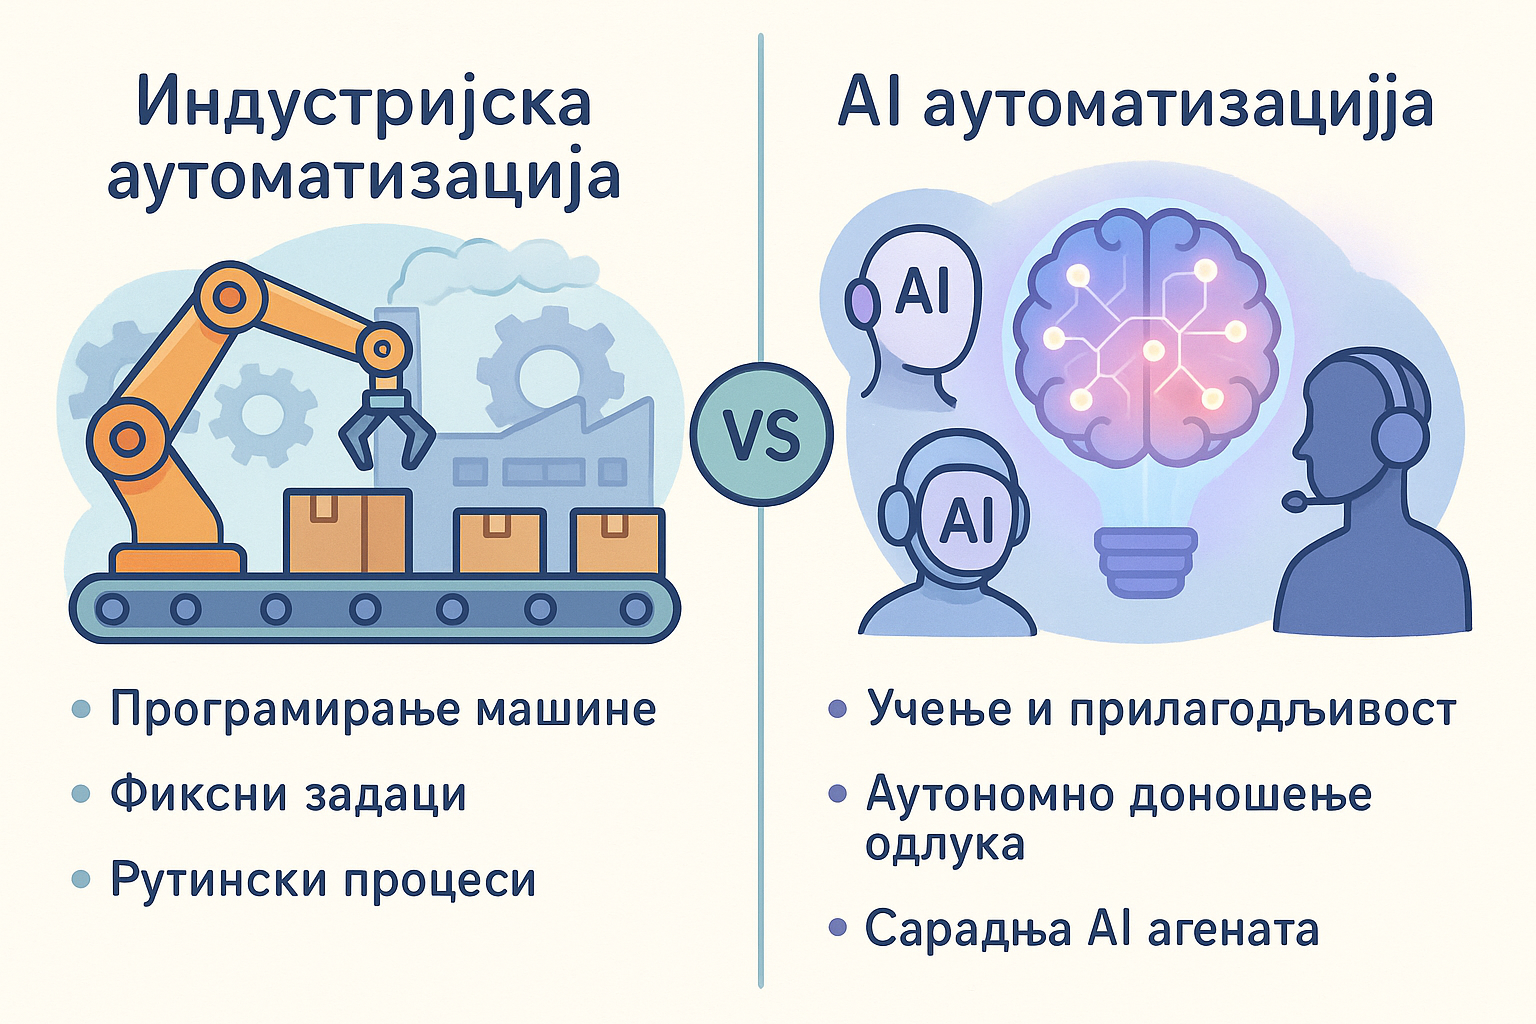
\includegraphics[width=0.95\textwidth]{slike/04/AI-Industrija.png}
    \caption{Поређење индустријске аутоматизације и AI аутоматизације}
    \label{fig:04-1}
\end{figure}

\subsubsection{Историјски развој: Од скрипти до когнитивних агената за одлучивање}

Да би се разумела тренутна парадигма, неопходно је сагледати еволутивни пут аутоматизације кроз три кључне фазе:

\begin{itemize}
    \item \textbf{Фаза 1: Скриптована аутоматизација (\textit{Scripting}).} \\
    Ово је најосновнији облик, резервисан за инжењере. Подразумева писање кода (Bash, Python, SQL) за извршавање једноставних, линеарних задатака (нпр. прављење резервне копије базе података сваке ноћи). Ови системи су ригидни; свака промена у окружењу доводи до прекида рада ("пуцања") скрипте.
    
    \item \textbf{Фаза 2: Роботска аутоматизација процеса (RPA).} \\
    RPA технологија омогућила је софтверу да имитира акције корисника на графичком интерфејсу (кликтање, куцање). Иако напреднија од скрипти, RPA и даље не разуме шта ради, већ само прати координате и правила. Ако се дугме на сајту помери за 5 пиксела, процес може стати~\cite{ivancic2019,wewerka2020rpa}.
    
    \item \textbf{Фаза 3: AI и Когнитивна аутоматизација (IPA).} \\
    Интеграцијом великих језичких модела (енг \textit{Large Language models - LLM})~\cite{brown2020,zhao2023llmsurvey}, аутоматизација добија способност "разумевања". Систем више не прати само координате, већ анализира семантичко значење. Ако се формат фактуре промени, AI агент и даље може препознати шта је нпр. датум, а шта износ, чинећи систем робусним и отпорним на промене.
\end{itemize}

Табела~\ref{tab:04-1} приказује кључне разлике између традиционалне аутоматизације засноване на правилима (RPA) и савремене AI аутоматизације. Традиционална аутоматизација функционише над строго структурираним подацима и ослања се на фиксна, унапред дефинисана правила, што је чини погодном за линеарне и понављајуће процесе са јасним улазно-излазним обрасцима. Такви системи су релативно једноставни за евалуацију, али захтевају интензивно одржавање, нарочито у случају промена пословних правила или структуре података.
Насупрот томе, AI аутоматизација је дизајнирана за рад са неструктурираним подацима, као што су текст, слике или глас, и карактерише је висока флексибилност захваљујући способности учења и прилагођавања. Ови системи уводе нелинеарне токове одлучивања и могу аутономно прилагођавати своје понашање на основу нових података и контекста. Иако такав приступ омогућава решавање знатно комплекснијих задатака, он истовремено отежава формалну евалуацију и захтева напредне методе валидације, интерпретабилности и надзора.


\begin{table}[h]
\centering
\caption{Компарација традиционалне и AI аутоматизације}
\vspace{0.3cm}
\begin{adjustbox}{max width=\textwidth}
\begin{tabular}{|p{5cm}|p{4.5cm}|p{4.5cm}|}
\hline
\textbf{Карактеристика} & \textbf{Традиционална (RPA)} & \textbf{AI Аутоматизација} \\
\hline
\textbf{Тип података} & Структурирани & Неструктурирани  \\
\hline
\textbf{Флексибилност} & Ниска (Фиксна правила) & Висока (Прилагодљива) \\
\hline
\textbf{Одржавање} & Захтевно  & Аутономно  \\
\hline
\textbf{Комплексност} & Линеарна & Нелинеарна \\
\hline
\textbf{Евалуација} & Лака & Тешка \\
\hline
\end{tabular}
\end{adjustbox}
\label{tab:04-1}
\end{table}

\subsubsection{"No-Code" револуција}

Један од најважнијих аспеката савремене аутоматизације, који се често наглашава у стручној литератури, јесте спуштање баријере уласка. До пре неколико година, изградња аутоматизованих агената захтевала је високо стручно знање из области софтверског инжењерства. Данас сведочимо успону тзв. \textbf{Citizen Developers} (Грађани-програмери). Захваљујући платформама као што су \textit{n8n}, \textit{Make} или \textit{Zapier}, процес програмирања је апстрахован кроз визуелне интерфејсе.

Уместо писања синтаксе кода, корисници креирају логику повезивањем визуелних блокова (чворова). Сваки чвор представља одређену функцију (нпр. „Прочитај email“, „Пошаљи Slack поруку“, „Питај ChatGPT“). Ово не значи да програмирање нестаје, већ да се фокус помера са \textit{sintakse} (како написати код) на \textit{logiku i arhitekturu} (шта систем треба да уради)~\cite{n8n,langchain}. Ово омогућава доменским експертима – људима из маркетинга, продаје, права или медицине – да сами граде алате који решавају њихове специфичне проблеме, без чекања на ИТ одељења.

\begin{quote}
\textit{"Аутоматизација више није алат за ИТ сектор, већ основна писменост модерног пословања у циљу прављења што бољих одлука."}
\end{quote}

Овај тренд доводи до брже итерације у пословању. Идеја се може претворити у функционалан прототип (MVP) за неколико сати, уместо за неколико недеља развоја, што радикално убрзава дигиталну трансформацију компанија. На слици~\ref{fig:04-2} задат је илустративни приказ "No-Code" револуције.

\begin{figure}[h!]
    \centering
    
\includegraphics[width=0.95\textwidth]{slike/04/nocode.png}
    \caption{"No-Code" револуција}
    \label{fig:04-2}
\end{figure}

% =================================================================================
% POGLAVLJE 1.2 - PROŠIRENA VERZIJA
% =================================================================================

\subsection{Стратешке предности имплементације аутоматизованих система}

Анализом савремених пословних процеса и студија случаја дигиталне трансформације, идентификован је низ стратешких и оперативних бенефита који произилазе из увођења AI аутоматизације. Ови бенефити превазилазе пуко смањење трошкова и дотичу се фундаменталне реорганизације начина на који се ствара вредност у компанији у циљу прављења што бољих одлука.

У наставку је дата детаљна анализа четири кључна стуба вредности аутоматизације.

\subsubsection*{1. Оперативна ефикасност и оптимизација људског капитала}

Најчешће помињан разлог за увођење аутоматизације је уштеда времена, међутим, у академском и менаџерском смислу, прецизније је говорити о \textbf{ре-алокацији когнитивних ресурса}.

У традиционалном моделу пословања, висококвалификовани запослени често троше између 30\% и 50\% свог радног времена на административне задатке ниске вредности (енг. \textit{Low-Value Tasks}), као што су:
\begin{itemize}
    \item Мануелни унос података из фактура у рачуноводствени софтвер.
    \item Копирање информација из емаилова у CRM системе.
    \item Организација састанака и усклађивање календара.
    \item Генерисање рутинских недељних извештаја.
\end{itemize}

Имплементацијом AI агената, ови процеси се делегирају машини. Ово доводи до феномена познатог као \textbf{"Когнитивно растерећење"} (\textit{Cognitive Offloading}). Када се запослени ослободи репетитивних радњи, његови капацитети се преусмеравају на послове високе вредности (енг. \textit{High-Value Work}):
\begin{itemize}
    \item Стратешко планирање: Анализа тржишних трендова и дефинисање дугорочних циљева.
    \item Креативно решавање проблема: Иновација производа и услуга.
    \item Емоционални рад: Изградња дубљих односа са кључним клијентима и управљање тимовима.
\end{itemize}

На основу наведеног може се извести једноставан закључак:
\begin{quote}
\textit{Економски посматрано, аутоматизација повећава повраћај на инвестицију (ROI) по запосленом, јер се цена радног сата човека троши на задатке које само човек може да обави, односно задатке које захтевају додатан интелектуални напор}
\end{quote}

\subsubsection*{2. Минимизација људске грешке и интегритет података}

Људски фактор је, статистички гледано, најслабија карика у процесима обраде података. Истраживања показују да при мануелном уносу података стопа грешке (типо, изостављање, погрешно поље) износи између 1\% и 4\%~\cite{vanderaalst2016}. Иако делује мало, у системима који обрађују хиљаде трансакција, ово доводи до значајних финансијских губитака и оперативних застоја.

Аутоматизовани системи уводе концепт \textbf{детерминистичког извршења}. То значи да ће софтверски агент, под истим условима, увек извршити задатак на идентичан начин.

Предности оваквог приступа су вишеструке:
\begin{itemize}
    \item \textbf{Конзистентност:} Податак који се аутоматски преноси из CRM система у ERP биће идентичан у 100\% случајева.
    \item \textbf{Усклађеност:} Аутоматизовани токови остављају дигитални траг (енг. \textit{Log files}). У индустријама попут банкарства или здравства, ово је кључно за ревизију и поштовање регулатива (као што је GDPR). Тачно се зна ко је (који агент), када и како обрадио податак.
    \item \textbf{Финансијска сигурност:} Елиминација грешака у фактурисању или обрачуну плата директно спречава одлив новца.
\end{itemize}

\subsubsection*{3. Скалабилност и еластичност пословања}

Један од највећих изазова за растуће компаније је тзв. "кочница људских ресурса". У мануелном моделу, раст обима посла линеарно прати раст трошкова радне снаге.
$$
\text{Обим посла} \uparrow \;\approx\; \text{Број запослених} \uparrow \;\approx\; \text{Трошкови} \uparrow
$$
Аутоматизација разбија ову линеарну зависност и омогућава експоненцијалну скалабилност. Софтверска инфраструктура поседује еластичност коју људска радна снага нема.

\textbf{Примери скалабилности:}
\begin{enumerate}
    \item \textbf{Управљање пиковима (Spikes):} Током периода као што је „Black Friday“, број упита корисника може порасти за 1000\%. Људски тим би био преплављен, што би довело до пада квалитета услуге. AI агенти могу тренутно скалирати своје капацитете (уз минимално повећање трошкова сервера) како би обрадили сав саобраћај без кашњења.
    \item \textbf{Микро-скалирање:} За мале бизнисе, аутоматизација омогућава да једна особа управља процесима за које би иначе био потребан тим од петоро људи (продаја, маркетинг, подршка, финансије).
\end{enumerate}

Ово омогућава компанијама да расту приходе много брже него што расту оперативни трошкови, чиме се повећава профитна маржа.

\subsubsection{Континуитет пословања (Концепт "Always-On")}

У глобалној дигиталној економији, концепт радног времена (9-до-5) постаје застарео. Потрошачи очекују инстант гратификацију и одговоре у реалном времену, без обзира на временску зону.

За разлику од биолошке радне снаге, дигитални радници (AI Агенти):
\begin{itemize}
    \item Не захтевају сан, одмор или паузе за ручак.
    \item Нису подложни паду концентрације услед замора.
    \item Не одлазе на боловања или годишње одморе.
\end{itemize}

Ово омогућава успостављање \textbf{континуитета пословања 24/7/365}.

\textbf{Практична импликација:}
Клијент из друге временске зоне (нпр. САД) може послати упит локалној фирми (нпр. у Србији) у 3 сата ујутру. Уместо да чека до 9 ујутру да запослени дође на посао, AI агент може:
\begin{enumerate}
    \item Тренутно анализирати упит.
    \item Проверити базу знања.
    \item Послати релевантан одговор или решити проблем (нпр. ресетовање лозинке).
    \item Заказати састанак у слободном термину запосленог за следећи дан.
\end{enumerate}

Резултат је драстично повећање задовољства корисника (енг. \textit{Customer Satisfaction}) и брже затварање продајних циклуса.


\subsection{Конзистентност и аналитика}

Аутоматизација намеће стандардизацију. Да би се процес аутоматизовао, он прво мора бити јасно дефинисан. Ово доводи до стварања конзистентних система који не зависе од индивидуалних навика запослених.

Додатно, аутоматизовани системи генеришу велику количину метаподатака. Уместо ручног прикупљања извештаја, менаџмент добија увид у перформансе система у реалном времену (енг. \textit{Real-time insights}), што омогућава доношење одлука заснованих на подацима (енг. \textit{Data-driven decision making}).

\subsection{Доменске области примене (\textit{Use Cases})}

Свестраност технологије AI аутоматизације омогућава њену имплементацију у готово свим порама модерног пословања. Ипак, анализа тржишта показује да се највећи повраћај на инвестицију (ROI) остварује у пет кључних пословних функција.

У наставку је дата детаљна дисекција примене аутоматизованих агената у овим вертикалама, са фокусом на трансформацију процеса из мануелних у аутономне.

\paragraph*{Продаја и управљање односима са клијентима (CRM)}
\noindent
CRM (енг. \textit{Customer Relationship Management}) системи представљају срце продајних организација, али су често неефикасни услед лошег квалитета података и неажурности продаваца. AI аутоматизација решава проблем шумовитих података и убрзава продајни циклус.

\begin{itemize}
    \item \textbf{Обогаћивање података о лидовима (Lead Enrichment):} \\
    Када корисник остави само емаил адресу на сајту, AI агент може аутоматски претражити јавне базе (LinkedIn, компанијске регистре), прикупити податке о позицији, величини фирме и индустрији, и ажурирати CRM профил пре него што продавац уопште види контакт.
    
    \item \textbf{Интелигентно бодовање лидова (AI Lead Scoring):} \\
    Уместо субјективне процене, алгоритми анализирају понашање корисника (отварање мејлова, посета страници са ценама) и аутоматски додељују приоритет~\cite{raffel2020t5,wolf2020transformers}. Агенти могу аутоматски заказати састанак само са оним клијентима који имају високу вероватноћу куповине, док остале стављају у процес едукације (nurturing).
    
    \item \textbf{Аутоматизовани Follow-up:} \\
    Статистика показује да је потребно просечно 5 до 7 контаката да би се закључила продаја. Људи често одустану након другог. AI агенти могу неуморно слати персонализоване секвенце порука (путем Емаил-а, LinkedIn-а или WhatsApp-а) све док не добију одговор, драстично повећавајући стопу конверзије.
\end{itemize}

\paragraph*{Корисничка подршка и искуство (Customer Support)}
\noindent
Ово је област где је примена AI највидљивија. Прелазак са класичних call-центара на хибридне AI системе мења парадигму подршке.

\begin{itemize}
    \item \textbf{Агенти првог нивоа (L1 Support):} \\
    AI агенти, оснажени RAG (енг. \textit{Retrieval Augmentation Generation}) архитектуром~\cite{lewis2020rag,gao2024ragsurvey}, могу решити између 60\% и 80\% рутинских упита (статус поруџбине, повраћај новца, основна техничка питања) без интервенције човека. За разлику од старих „chatbot-ова“ са фиксним менијима, ови агенти разумеју природни језик и контекст.
    
    \item \textbf{Анализа сентимента и приоритизација:} \\
    Приликом пријема тикета, AI анализира тон поруке. Ако детектује фрустрацију или бес ("Љутит клијент"), систем аутоматски ескалира тикет директно менаџеру подршке, заобилазећи стандардну процедуру чекања.
    
    \item \textbf{Omnichannel синхронизација:} \\
    Агенти прате интеракције на свим каналима. Ако се корисник жалио на Twitter-у, а затим послао емаил, систем препознаје да је то иста особа и исти проблем, омогућавајући агенту подршке увид у комплетну историју комуникације.
\end{itemize}

\paragraph{Маркетинг операције и генерисање садржаја}
\noindent
Маркетинг је еволуирао из креативне у техничко-креативну дисциплину. Аутоматизација омогућава хипер-персонализацију на скали коју људи не могу постићи.

\begin{itemize}
    \item \textbf{Генерисање и варијација садржаја:} \\
    Коришћењем генеративних модела, аутоматизација може креирати стотине варијација огласа (текст и слика) прилагођених различитим циљним групама. Агент може написати блог пост, затим га аутоматски претворити у LinkedIn објаву, Twitter низ (thread) и скрипту за TikTok видео.
    
    \item \textbf{Системи препоруке:} \\
    Уместо слања истог newsletter-а свима, систем аутоматски сегментира базу на основу понашања. Ако је корисник кликнуо на линк о „AI алатима“, аутоматски улази у секвенцу која му шаље више садржаја на ту тему.
    
    \item \textbf{Social Listening и реакција:} \\
    AI агенти могу 24/7 пратити помињање бренда на интернету. У случају негативног помињања, могу алармирати PR тим, или у случају позитивног, аутоматски лајковати и захвалити се кориснику.
\end{itemize}

\paragraph{Финансијски менаџмент и рачуноводство}
\noindent
Финансијски сектор захтева прецизност и усклађеност са прописима, што га чини идеалним кандидатом за детерминистичку аутоматизацију.

\begin{itemize}
    \item \textbf{Аутоматизација обраде фактура (Accounts Payable):} \\
    AI агенти користе OCR (енг. \textit{Optical Character Recognition}) да прочитају PDF фактуре које стижу на емаил, екстрахују податке (добављач, износ, ПИБ), провере да ли се слажу са наруџбеницом и аутоматски их унесу у рачуноводствени софтвер или припреме налог за плаћање~\cite{schwab2017}.
    
    \item \textbf{Упаривање трансакција (Reconciliation):} \\
    Упоређивање банковних извода са интерним књиговодством је мукотрпан процес. Аутоматизација може у секундама упарити хиљаде ставки и издвојити само оне које се не слажу (аномалије) за људску ревизију.
    
    \item \textbf{Управљање трошковима:} \\
    Запослени могу сликати рачун телефоном, а AI агент аутоматски категоризује трошак, проверава да ли је у складу са политиком фирме и шаље на одобрење.
\end{itemize}

\paragraph{Управљање пројектима и HR процеси}

Интерна ефикасност организације директно зависи од брзине протока информација.

\begin{itemize}
    \item \textbf{Аутоматизовани Onboarding запослених:} \\
    Када се у HR систему означи да је нови запослени примљен, агент аутоматски: креира email налог, додаје га у релевантне Slack канале, шаље уговор на потписивање, заказује уводне састанке и шаље материјале за обуку.
    
    \item \textbf{Праћење статуса пројеката:} \\
    Уместо дугих састанака за „статус update“, AI агент може на крају дана питати сваког члана тима „Шта си данас урадио?“ путем chat-а, сумирати све одговоре и послати менаџеру консолидовани извештај о напретку пројекта.
\end{itemize}


\newpage

% =================================================================================
% POGLAVLJE 2
% =================================================================================

\section{Техничка инфраструктура аутоматизације}
\label{sec:tehnicka-infrastruktura}

У претходном поглављу разматрани су концептуални и стратешки аспекти AI аутоматизације, са фокусом на пословну вредност,
доменске примене и организационе импликације. Међутим, како би аутоматизација прешла из теоријског оквира у реалну,
продукцијску примену, неопходно је детаљно разумети техничку инфраструктуру која такве системе чини могућим.

Техничка инфраструктура аутоматизације представља скуп међусобно повезаних софтверских компоненти које омогућавају:
детекцију догађаја, оркестрацију процеса, размену података између хетерогених система, доношење интелигентних одлука
и надзор над извршавањем у реалном времену~\cite{omg2014bpmn,vanderaalst2016}. За разлику од класичних информационих система, где су токови често
тврдо кодирани и монолитни, савремени аутоматизовани системи су дистрибуирани, догађајима вођени и високо модуларни.

Посебан изазов у пројектовању оваквих система представља интеграција компоненти вештачке интелигенције.
AI модели, нарочито велики језички модели, нису детерминистички по својој природи и не могу се посматрати као
једноставна замена за традиционални програмски код. Због тога је неопходно увести јасну архитектонску структуру
у којој AI функционише као контролисана и надзирана компонента унутар ширег аутоматизованог тока.

У овом поглављу биће представљена референтна техничка архитектура AI аутоматизације, као и кључни инфраструктурни
концепти који омогућавају њену поуздану, скалабилну и безбедну примену у пракси. Посебан акценат биће стављен
на улогу оркестрације, интеграција, управљања подацима и обсервабилити слоја, уз илустрацију кроз савремене
workflow алате који омогућавају визуелно моделовање комплексних процеса.


\subsection{Референтна архитектура аутоматизације}
\label{sec:ref_arch}

Техничка инфраструктура AI аутоматизације може се посматрати као слојевита архитектура која комбинује:
(и) механизме за \textit{детекцију догађаја} (тригери), (ии) систем за \textit{orkestraciju toka rada} (workflow engine),
(иии) интеграције са спољним сервисима путем API-ја, (ив) слој за управљање подацима, и (в) AI слој који доноси
одлуке и генерише садржај на основу контекста.

У пракси, ове компоненте не чине монолит, већ модуларан систем у коме се сваки слој може независно заменити
или унапредити. Такав приступ је кључан за одрживост аутоматизације: процеси се временом мењају, уводе се нови алати,
а промена једног сервиса (нпр. CRM система) не би смела да уруши читав аутоматизовани ток.

\subsubsection{Слојеви референтне архитектуре}

У наставку су описани основни слојеви референтне архитектуре аутоматизације. Сваки слој представља логичку целину,
док се у имплементацији често преклапају или спајају у зависности од величине система.

\paragraph*{1. Trigger слој (иницирање процеса)}
Trigger слој је улазна тачка аутоматизације: он детектује догађај и покреће ток рада. Типични окидачи су:
\begin{itemize}
    \item \textbf{Ручни тригер:} ово представља ручни тригер за окидање и извршавање тока рада.
    \item \textbf{Webhook догађаји:} нпр. нова поруџбина у web shop-у или нова пријава кроз форму.
    \item \textbf{Scheduler (временски окидач):} нпр. стартовање тока рада сваког понедељка у 08:00.
    \item \textbf{Inbox / поруке / чет порука:} нпр. пријем емаила у специфично сандуче, нова порука у chat каналу.
    \item \textbf{Системски догађаји:} нпр. промена у бази података или нови фајл у фолдеру (Google Drive trigger).
\end{itemize}

У индустријским системима, начин иницирања процеса директно утиче на латенцију и поузданост~\cite{airflow}.
Webhook приступ омогућава реакцију у реалном времену, док scheduler и ручни тригери имају веће кашњење,
али могу бити једноставнији за имплементацију у окружењима где webhook-ови нису доступни. На слици~\ref{fig:04-3} задат је илустративни приказ тригера у \textit{n8n} .

\begin{figure}[h!]
    \centering
    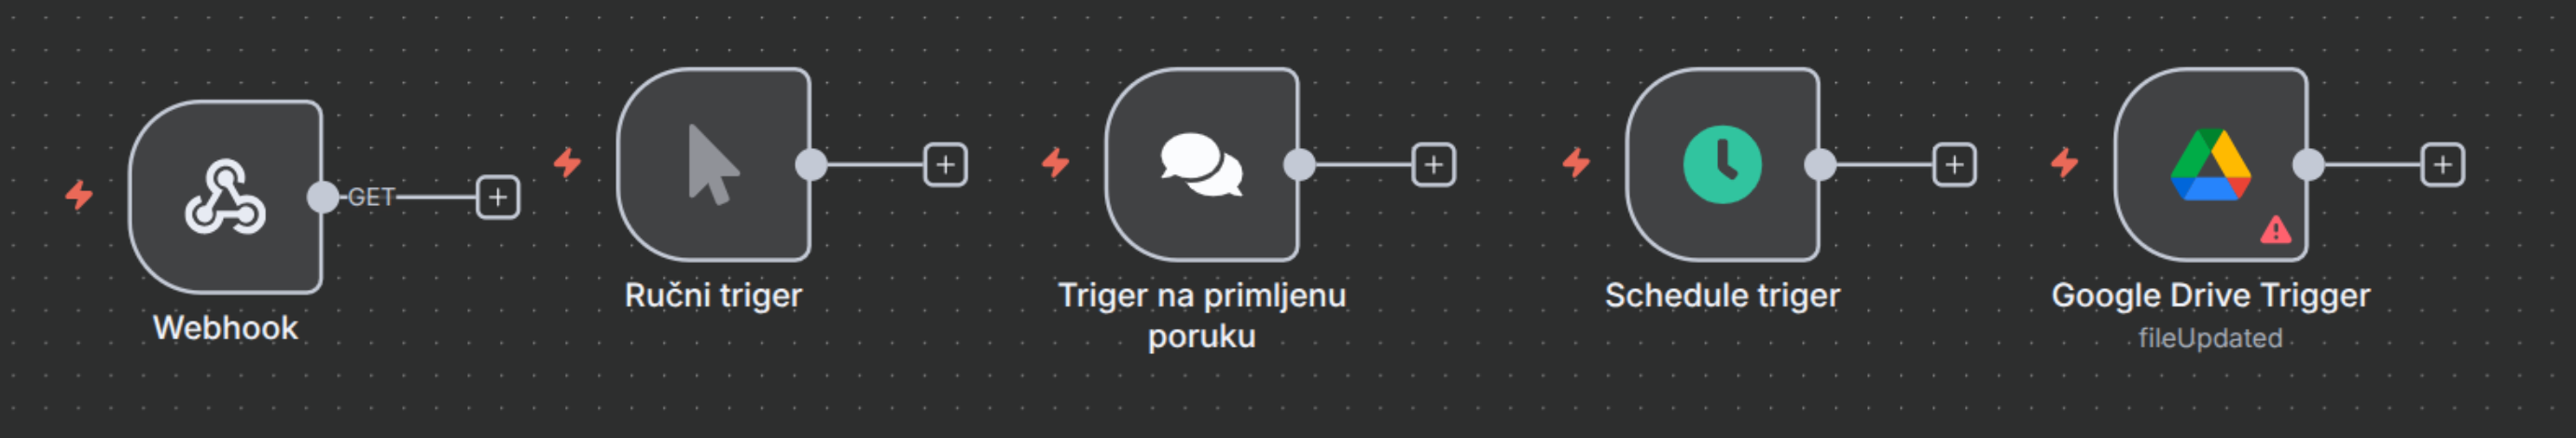
\includegraphics[width=0.95\textwidth]{slike/04/Trigeri.png}
    \caption{Илустративан приказ тригер иконица у \textit{n8n}}
    \label{fig:04-3}
\end{figure}

\paragraph*{2. Orchestration слој (workflow engine)}
Оркестрациони слој је \textit{centralni dirigent} аутоматизације. Његова улога је да:
\begin{itemize}
    \item управља редоследом корака (секвенца),
    \item доноси одлуке о гранању (иф/свитцх),
    \item координира паралелне активности,
    \item имплементира ретри/бацкофф када дође до грешке,
    \item чува контекст извршавања (нпр. \textit{run id}, стање процеса),
    \item логује резултате и грешке по корацима.
\end{itemize}

Генерално оркестрација се често демонстрира кроз алате типа \textit{n8n}, где су кораци представљени чворовима
који се повезују у граф процеса. Међутим, важно је нагласити да је оркестрација концептуално независна од алата:
workflow engine може бити и цустом микросервис, платформа или чак сет серверлесс функција повезаних догађајима~\cite{airflow,omg2014bpmn}. На слици~\ref{fig:04-4} задат је илустративни приказ тригера у \textit{n8n} .

\begin{figure}[h!]
    \centering
    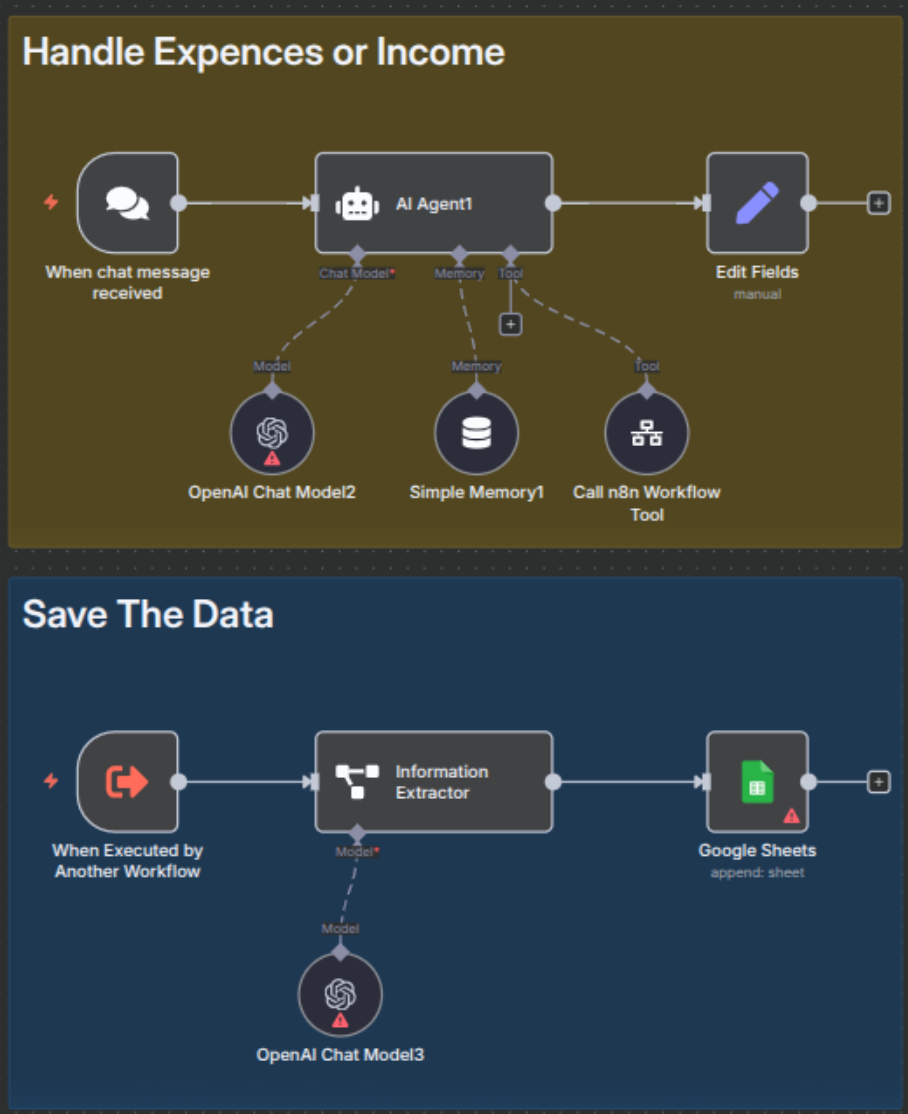
\includegraphics[width=0.8\textwidth]{slike/04/workflow_example.png}
    \caption{Илустративан приказ тока рада у \textit{n8n}}
    \label{fig:04-4}
\end{figure}


\paragraph*{3. Интеграциони слој (конектори и API комуникација)}
Интеграциони слој представља \textbf{спојно ткиво} аутоматизованог система и његовог спољног окружења.
Његова основна улога је да омогући поуздану, сигурну и стандардизовану размену података између аутоматизованог
workflow-а и различитих софтверских система који учествују у пословном процесу. Ови системи могу бити интерни
(CRM, ERP, базе података) или екстерни (паимент процесори, SaaS алати, државне платформе, аналитички сервиси).

У савременим информационим системима интеграција се готово искључиво ослања на API-је
(енг. \textit{Application Programming Interfaces}), који дефинишу како један софтверски систем излаже своје функционалности
другима. Аутоматизовани агент у том контексту преузима улогу клијента који шаље захтеве, прима одговоре и
тумачи их у складу са пословном логиком.

\paragraph*{Типови интеграционих интерфејса}

Најзаступљенији облик интеграције је \textbf{REST API}, где се размена података одвија путем HTTP протокола,
а операције су мапиране на стандардне HTTP методе:
\begin{itemize}
    \item \texttt{GET} – дохват података,
    \item \texttt{POST} – креирање нових записа или покретање акција,
    \item \texttt{PUT/PATCH} – измена постојећих записа,
    \item \texttt{DELETE} – брисање ресурса.
\end{itemize}

Поред REST-а, у одређеним доменима користе се и:
\begin{itemize}
    \item \textbf{GraphQL API}: омогућава флексибилно дефинисање тачно оних поља која су потребна,
    чиме се смањује количина пренетих података и број захтева.
    \item \textbf{SOAP сервиси}: и даље присутни у банкарским и државним системима, са строго дефинисаним шемама (WSDL).
    \item \textbf{SDK-ови и проприетарни интерфејси}: библиотеке које врше директну комуникацију са специфичним сервисима.
\end{itemize}

У контексту аутоматизације, избор интерфејса директно утиче на комплексност workflow-а, латенцију
и могућност детекције грешака.
У пракси, ови интерфејси се у оквиру аутоматизованих система често реализују кроз визуелне оркестрационе алате,
као што је \textit{n8n}, где је сваки API позив енкапсулиран у посебан чвор (ноде).
Такви чворови апстрахују нисконивојске детаље комуникације (HTTP методе, заглавља, аутентификацију),
док пројектанту процеса остављају фокус на логику тока, обраду одговора и руковање грешкама.
На овај начин, комплексне интеграције између хетерогених система могу се моделовати, тестирати и мењати
без потребе за писањем опсежног програмског кода, што значајно убрзава развој и одржавање аутоматизованих workflow-а.



\paragraph*{4. Дата слој (управљање подацима и меморија система)}
Дата слој обезбеђује да аутоматизација има стабилан ослонац у подацима. У најједноставнијем случају,
то може бити једна релациона база. У напредним системима разликују се најмање четири типа складишта:
\begin{itemize}
    \item \textbf{Оперативна база (OLTP):} нпр. PostgreSQL за трансакционе податке.
    \item \textbf{Документ складиште:} нпр. NoSQL база или фајл стораге за неструктуриране документе (PDF, слике).
    \item \textbf{Аналитичко складиште (OLAP):} агрегације, извештаји и БИ.
    \item \textbf{Векторска база:} складиштење embedding-а ради семантичке претраге (RAG системи)~\cite{johnson2019faiss,reimers2019sbert}.
\end{itemize}

Улога дата слоја је двострука: (и) чување резултата процеса (нпр. упис у CRM) и (ии) обезбеђивање контекста
за одлучивање (нпр. историја поруџбина клијента, правила, претходне комуникације). Дата слој је неопходан како би се агенти потхрањивали подацима. Примери чворова који представљају дата слој у \textit{n8n} дати су на слици~\ref{fig:04-5} 

\begin{figure}[h!]
    \centering
    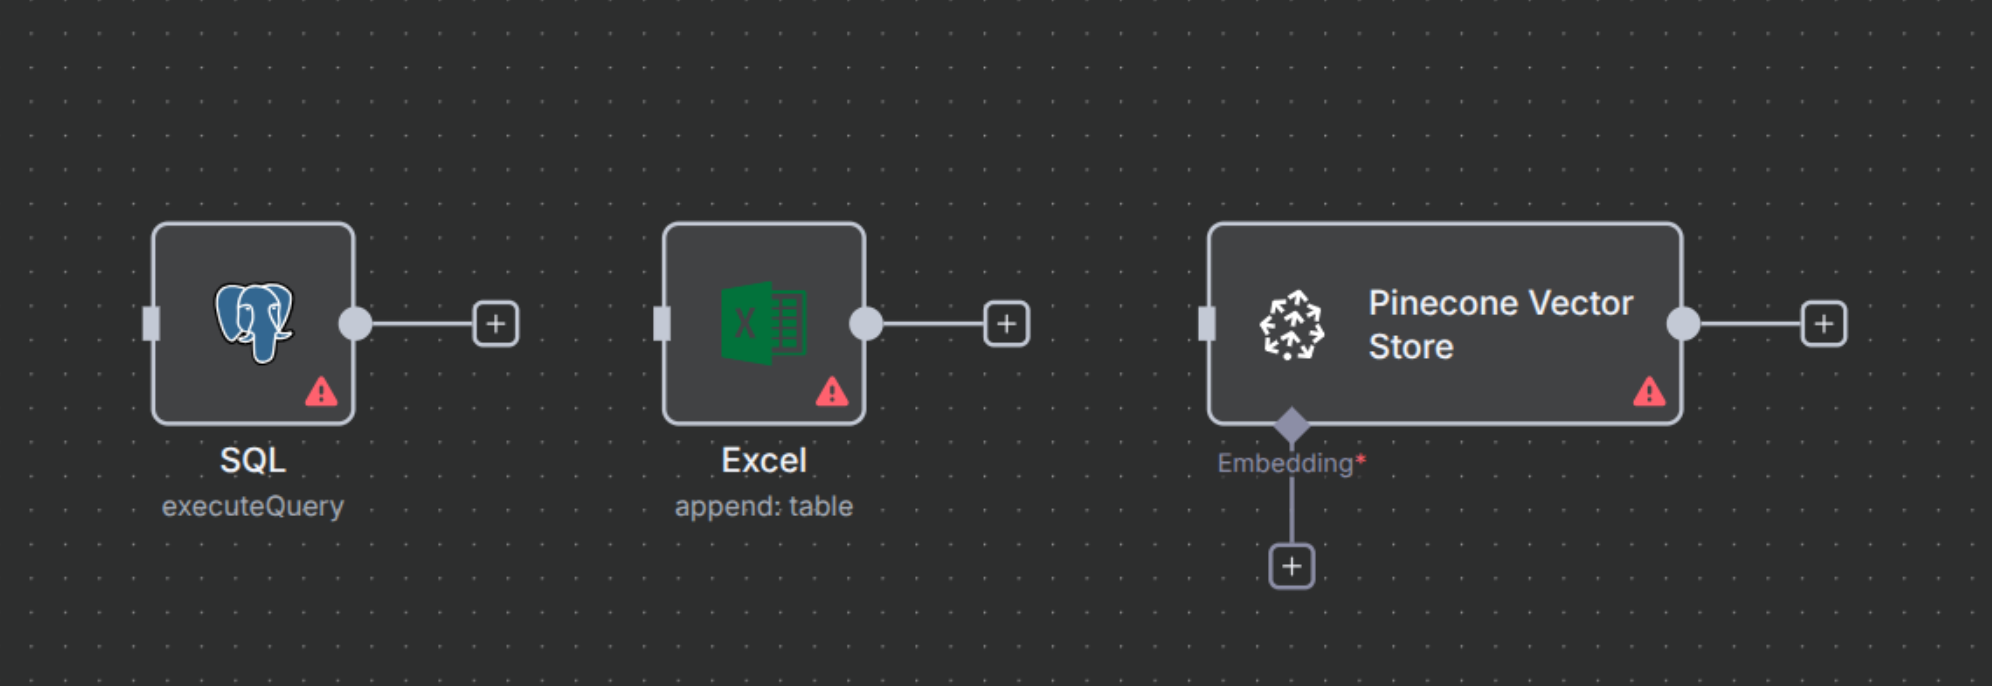
\includegraphics[width=0.8\textwidth]{slike/04/DB.png}
    \caption{Илустративан приказ тока рада у \textit{n8n}}
    \label{fig:04-5}
\end{figure}

\paragraph*{5. AI слој (модели, одлуке и генерисање)}
AI слој уводи способности које класична аутоматизација нема: разумевање текста, класификацију намере,
екстракцију информација из докумената, генерисање одговора и препорука~\cite{zhao2023llmsurvey}.

Типичне компоненте AI слоја укључују:
\begin{itemize}
    \item \textbf{LLM модели:} генерисање текста, сумирање, класификација и tool-calling~\cite{brown2020,schick2023toolformer}.
    \item \textbf{Embedding модели:} претварање текста/докумената у векторе за семантичку претрагу~\cite{mikolov2013,reimers2019sbert}.
    \item \textbf{OCR/VLM модели:} рад са сликама и документима (фактуре, уговори, формулари), као и \textit{Speech-to-Text} модели за обраду гласа~\cite{radford2022whisper}.
    \item \textbf{RAG архитектура:} комбиновање претраге знања и генерисања одговора~\cite{lewis2020rag}.
\end{itemize}
\noindent
Важно је нагласити да AI слој није замена за оркестрацију и интеграције, већ функционише као \textit{inteligentna komponenta}
унутар већег детерминистичког процеса. У добро пројектованом систему, AI делује унутар јасно дефинисаних граница:
добија контролисани input, генерише структурисан output, и пролази кроз валидацију пре него што утиче на спољашњи свет.

\paragraph*{6. Guardrails и контрола (валидација, сигурност и усклађеност)}

Како аутоматизација постепено преузима оперативне и одлучивачке задатке
(нпр. слање екстерних комуникација, креирање налога, иницирање финансијских трансакција),
неопходно је увести слој контроле који ограничава понашање система и спречава нежељене или
штетне последице~\cite{bai2022,hleg2019}. Овај слој, познат као \textbf{Guardrails}, представља скуп техничких и
организационих механизама који дефинишу границе дозвољеног деловања аутоматизованих агената. За разлику од класичних софтверских система, код којих је понашање детерминистички дефинисано
програмским кодом, системи засновани на вештачкој интелигенцији, а нарочито на великим језичким
моделима (LLM), производе генеративни излаз који може варирати у зависности од контекста.
Због тога контрола оваквих система захтева вишеслојни приступ.

\paragraph{Валидација излаза и структурална контрола}

Први ниво заштите односи се на проверу да ли је излаз система у складу са очекиваним форматом
и пословним правилима. У пракси се често користи:
\begin{itemize}
    \item валидација према унапред дефинисаним шемама (нпр. JSON Schema),
    \item провера типова података, опсега вредности и обавезних поља,
    \item одбацивање или корекција излаза који не задовољавају формалне критеријуме.
\end{itemize}

Овим приступом се спречава да генеративни модел произведе синтактички исправан, али
структурно неупотребљив или опасан резултат.

\paragraph{Политике понашања и домен дозвољених одговора}

Други ниво контроле чине експлицитне \textbf{политике и правила понашања}.
Оне дефинишу:
\begin{itemize}
    \item које врсте акција агент сме да изврши (нпр. слање информативних, али не и правно обавезујућих порука),
    \item на која питања сме да даје одговоре, а на која мора да одбије или ескалира захтев,
    \item границе доменског знања у оквиру којих агент може аутономно деловати.
\end{itemize}

У пословним системима, ове политике су често усклађене са интерним правилницима,
регулаторним захтевима и етичким смерницама организације.

\paragraph{Заштита осетљивих података и усклађеност}

Аутоматизовани системи често обрађују личне и поверљиве информације.
Због тога је маскирање и контрола осетљивих података (енг. \textit{Personally Identifiable Information -- PII})
од кључног значаја. Типичне мере укључују:
\begin{itemize}
    \item анонимизацију или псеудонимизацију података пре слања AI моделу,
    \item уклањање осетљивих информација из логова и промптова,
    \item строго ограничавање приступа подацима у складу са принципом најмањих привилегија,
    \item одбрану од индиректних напада кроз промпт-ињекцију, где злонамерни садржај у дохваћеним документима преусмерава понашање агента~\cite{greshake2023injection}.
\end{itemize}

Ове мере омогућавају усклађеност са регулативама као што су GDPR и интерне политике безбедности.

\paragraph{Human-in-the-loop и ескалација}

За акције са потенцијално високим ризиком (нпр. финансијске трансакције, раскид уговора,
слање правно осетљивих порука), аутоматизација се не ослања искључиво на аутономне одлуке.
Уместо тога, уводи се концепт \textbf{Human-in-the-loop}, где:
\begin{itemize}
    \item систем припрема предлог одлуке или акције,
    \item човек врши финалну проверу и одобрење,
    \item одлука се затим извршава или одбацује.
\end{itemize}

Овакав приступ комбинује ефикасност аутоматизације са одговорношћу и проценом човека.

\noindent
Закључно, Guardrails слој је кључни предуслов за безбедну и поуздану примену AI аутоматизације.
Он обезбеђује да интелигентни системи остану под контролом, чак и у ситуацијама непредвиђеног
понашања модела или промена у контексту.

\paragraph*{7. Опсервациони слој (логови и метрике)}

Без адекватног увида у рад система, аутоматизација постаје нетранспарентна,
тешка за одржавање и непоуздана у продукционом окружењу.
Observability слој омогућава континуирано праћење понашања аутоматизованих токова рада
и представља основ за дијагностику, оптимизацију и дугорочну стабилност система.

За разлику од класичног мониторинга, који се фокусира на основне показатеље доступности,
обсервабилити тежи разумевању \textit{зашто} је систем у одређеном стању.

\paragraph{Логовање извршавања}

Логови представљају хронолошки запис извршавања аутоматизованог процеса.
У контексту AI аутоматизације, логовање обухвата:
\begin{itemize}
    \item улазне податке и излазе по кораку workflow-а,
    \item статус извршења (успех, грешка, ретри),
    \item контекстуалне информације (време, идентификатор процеса).
\end{itemize}
\noindent
Како логови могу садржати осетљиве податке, неопходно је применити редакцију и селективно
чување информација, у складу са безбедносним и регулаторним захтевима.

\paragraph{Метричке и квантитативна анализа}

Метричке омогућавају квантитативну процену перформанси аутоматизације.
Најчешће праћени показатељи укључују:
\begin{itemize}
    \item стопу успешности извршавања,
    \item просечну и максималну латенцију по кораку,
    \item број и учесталост ретри покушаја,
    \item проценат грешака по интеграцији или функцији.
\end{itemize}
\noindent
Анализом ових података могуће је идентификовати уска грла, деградацију перформанси
или промене у понашању система током времена.

\paragraph{Alerting и проактивно реаговање -}

На основу прикупљених метрика дефинишу се прагови и услови за алармирање.
Када систем прекорачи дозвољене вредности (нпр. нагли пораст грешака или кашњења),
аутоматски се генеришу обавештења према оперативним тимовима.
\noindent
Овај механизам омогућава проактивну реакцију, пре него што проблем постане видљив
крајњим корисницима или утиче на пословне резултате.

\paragraph{Tracing и анализа токова извршавања -}

У сложеним, дистрибуираним системима, један аутоматизовани процес често обухвата
више сервиса и интеграција. Tracing омогућава праћење једне извршне инстанце
кроз све компоненте система, од иницијалног окидача до завршетка процеса.

Овај приступ је посебно важан за:
\begin{itemize}
    \item идентификацију узрока спорог извршавања,
    \item анализу ланаца грешака,
    \item разумевање зависности између појединачних корака.
\end{itemize}

\noindent
Управо обсервабилити слој омогућава прелазак са експерименталних прототипова
на стабилне, скалабилне и поуздане продукционе системе, чиме AI аутоматизација
постаје дугорочно одржива компонента пословне инфраструктуре.

\subsubsection{Сажетак: Од прототипа до продукције и доношења одлука}

Референтна архитектура аутоматизације служи као практичан и методолошки оквир за пројектовање
аутоматизованих система различитих величина и степена сложености. У раној фази развоја,
односно приликом израде прототипа или минимално одрживог производа (MVP),
често је прихватљиво објединити више архитектонских слојева у један алат или платформу
(нпр. оркестрација процеса, управљање подацима и позивање AI модела унутар јединственог окружења
као што су workflow алати у комбинацији са LLM API сервисима).
Међутим, како аутоматизовани систем прелази из експерименталне у продукциону фазу
и постаје критична компонента пословних процеса, овакав приступ постаје ограничавајући.
Раст обима података, повећање броја интеграција и већи захтеви у погледу поузданости и безбедности
намећу потребу за јасном модуларизацијом архитектуре.
У тој фази долази до раздвајања слојева за оркестрацију, податке и интеграције,
увођења наменског обсервабилити слоја за праћење перформанси и грешака,
као и јачања гуардраилс механизама који ограничавају и надзиру понашање система.

Посебну пажњу у овом прелазу захтева интеграција компоненти вештачке интелигенције.
AI модели се више не третирају као изоловани експериментални модули,
већ као контролисани подсистеми који функционишу унутар детерминистичких токова рада,
уз јасно дефинисане улазе, излазе и механизме валидације.
На тај начин се постиже баланс између флексибилности коју AI доноси
и стабилности која је неопходна за поуздану продукциону примену.
На Слици~\ref{fig:04-6} приказан је илустративни преглед слојева референтне архитектуре аутоматизације,
од иницијалних окидача и оркестрације процеса, преко интеграција и контролних механизама,
до слоја за посматрање и анализу рада система.
Приказана шема има концептуални карактер и служи као водич за разумевање односа између компоненти,
док се конкретна имплементација може прилагођавати техничким и организационим захтевима конкретног система.

\begin{figure}[h!]
    \centering
    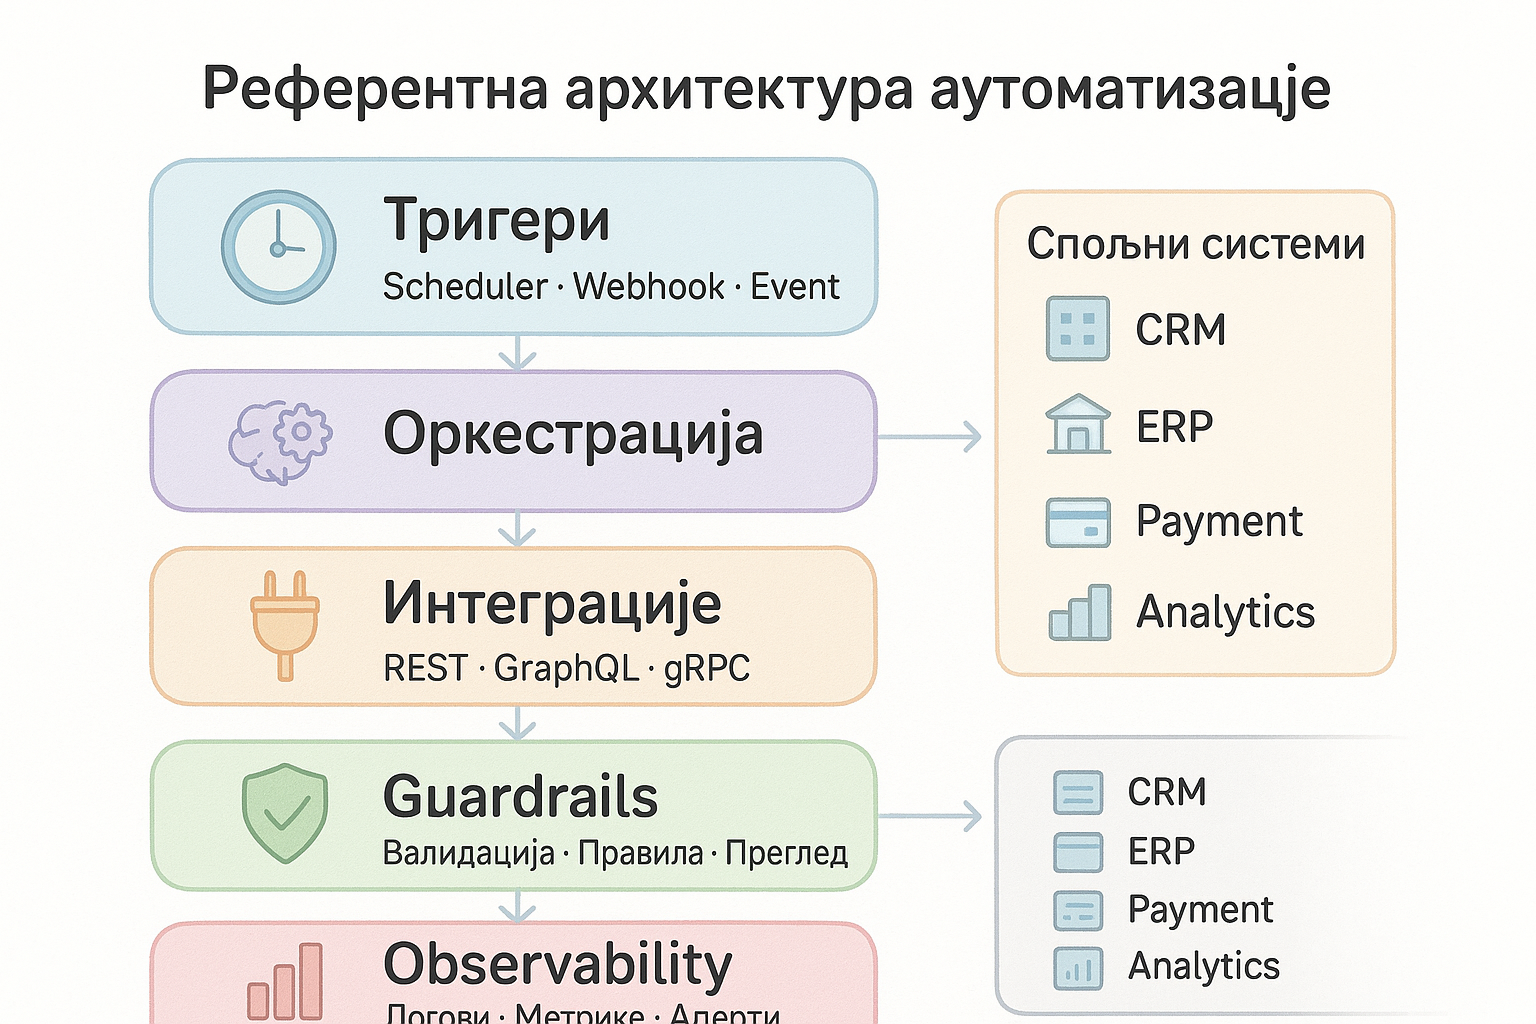
\includegraphics[width=0.95\textwidth]{slike/04/workflow_arcitekture.png}
    \caption{Референтна архитектура аутоматизације: слојеви и ток информација}
    \label{fig:04-6}
\end{figure}

\newpage

% =================================================================================
% POGLAVLJE 3
% =================================================================================

\section{Таксономија и Архитектура AI Система}
\label{sec:taksonomija-ai}

Развој савремених AI система захтева много више од избора „правог“ великог језичког модела (LLM).
Кључ успешне имплементације не лежи у самом моделу, већ у разумевању степена аутономије који систем треба да поседује и у архитектури која тај степен аутономије омогућава на контролисан и безбедан начин.
У пракси, један од најчешћих проблема у комуникацији између инжењера, менаџмента и клијената јесте
терминолошка конфузија. Појмови попут \textit{chatbota}, \textit{RAG sistema} и \textit{AI agenata} често се користе као синоними, иако представљају фундаментално различите архитектурне приступе.
Последица тога су нереална очекивања (нпр. да chatbot „сам нешто уради“) или, са друге стране,
прекомерно сложена решења за једноставне проблеме.

Ово поглавље уводи таксономију AI система засновану на нивоу аутономије и одговорности система.
Уместо да се AI посматра као монолитна технологија, системи се класификују дуж континуума:
од пасивних, реактивних модела који само генеришу текст, до комплексних, вишекомпонентних система
способних за планирање, извршавање акција и сарадњу са другим агентима.

Посебан фокус стављен је на разлику између:
\begin{itemize}
    \item Генеративних способности - шта систем може да напише,
    \item Оперативних способности - шта систем може да уради,
    \item Степена одговорности - који систем преузима у реалном окружењу.
\end{itemize}
\noindent
Како се крећемо ка вишим нивоима аутономије, AI системи престају да буду само алати за подршку кориснику,
а постају активни учесници у пословним и техничким процесима.
Са тим растом моћи пропорционално расте и потреба за јасном архитектуром, контролом тока извршења,
управљањем стањем, као и механизмима за опоравак од грешака.

Структура поглавља прати ову прогресију и уводи четири јасно раздвојена нивоа:
\begin{enumerate}
    \item AI асистенте у потпуности ослоњени ка LLM закључивање,
    \item RAG системе који додају утемељење у реалним подацима,
    \item Аутономне агенте способне за доношење одлука и извршавање акција,
    \item Мулти-агентске системе који омогућавају оркестрацију и колективно решавање сложених проблема.
\end{enumerate}
\noindent
Циљ овог поглавља није да промовише „најнапреднији“ приступ, већ да пружи инжењерски оквир за доношење
исправне одлуке: \textit{који ниво архитектуре је довољан, а који је непотребно сложен за конкретан проблем}.


\subsubsection*{Ниво 1: AI Асистенти (LLM закључивање)}

AI Асистенти представљају најосновнији и најраширенији облик примене генеративне вештачке интелигенције.
Они су примарно дизајнирани као интерфејси за закључивање над великим језичким моделима (LLM),
без трајног памћења, без аутономије и без директног утицаја на спољашње системе.
У архитектонском смислу, AI асистент је типично стателесс сервис:
сваки кориснички упит се обрађује независно, а сав „контекст“ који модел користи мора бити експлицитно
прослеђен унутар самог захтева (промпт-а).
Модел не поседује сопствено стање које се одржава између сесија, нити разуме континуитет интеракције
изван онога што му је тренутно дато као улаз.
Због тога се овај ниво често описује као примена LLM-а над текстом, приликом чега се
изводи пробабилистичко закључивање и враћа генерисани текст као одговор.
Примери таквих система су општи AI асистенти базирани на моделима попут GPT-4.1, Claude 4.5 или Qwen 3,
када се користе без додатне инфраструктуре (меморије, алата или екстерних извора података).

Иако је кориснички доживљај често антропоморфан (модел делује као да „разуме“, „зна“ или „размишља“),
унутрашњи механизам рада је знатно једноставнији, али математички софистициран~\cite{bender2021}.
AI асистенти функционишу на принципу предикције наредног токена (енг. \textit{Next Token Prediction})~\cite{vaswani2017,brown2020}.
За дати низ претходних токена (речи, делова речи или симбола), модел рачуна вероватноће могућих наредних
токена и бира следећи токен на основу тих вероватноћа.
Овај процес се понавља итеративно док се не генерише комплетан одговор.

Кључно је нагласити да модел:
\begin{itemize}
    \item не поседује унутрашњи појам истинитости или лажности,
    \item не проверава чињенице у реалном времену,
    \item не разликује „знање“, „претпоставку“ и „измишљање“ на концептуалном нивоу.
\end{itemize}
\noindent
За модел, тврдње попут „Париз је главни град Француске“ и „Париз је главни град Немачке“ нису
логички објекти са вредношћу истине, већ секвенце токена са различитим вероватноћама појављивања
у сличним контекстима током тренинга.

Овакав начин рада намеће неколико фундаменталних ограничења која су заједничка свим AI асистентима
на овом нивоу аутономије.

\begin{itemize}
    \item \textbf{Замрзнуто знање (Static Knowledge):}
    LLM модели не „уче“ након завршетка тренинга.
    Њихово знање је временски ограничено тренутком пресека података коришћених за тренирање.
    Догађаји, промене прописа, цене, или интерни документи који су настали након тог тренутка
    за модел не постоје, осим ако нису експлицитно унети у промпт.

    \item \textbf{Халуцинације:}
    Када модел нема довољно информација да поуздано одговори, он не сигнализира незнање
    на људски начин, већ наставља процес генерисања текста~\cite{ji2023hallucination}.
    Резултат су одговори који су лингвистички уверљиви, граматички исправни и често стилистички
    ауторитативни, али чињенично нетачни.
    Ово понашање није грешка у имплементацији, већ директна последица пробабилистичке природе модела.

    \item \textbf{Изолованост (Sandbox):}  
    Стандардни AI асистент нема приступ спољашњем свету.
    Он не види базе података, не приступа интернету, не може да провери стање система нити да
    изврши акцију.
    Све информације којима располаже морају бити садржане у самом упиту или већ присутне у
    параметрима модела из тренинга.
\end{itemize}
\noindent
Ова ограничења чине AI асистенте пасивним системима:
они реагују на кориснички унос, али не иницирају активности, не доносе одлуке које имају последице
у реалном окружењу и не сносе оперативну одговорност.

Упркос наведеним ограничењима, AI асистенти су изузетно корисни када се користе у правом контексту.
Њихова снага лежи у раду са текстом и симболима, а не у интеракцији са реалним системима.

Типичне и оправдане примене овог нивоа укључују:
\begin{itemize}
    \item креативно и техничко писање,
    \item сумирање и реструктурирање текста који корисник обезбеди,
    \item превођење између природних језика,
    \item помоћ при програмирању (code suggestions, објашњења, рефакторисање),
    \item генерисање идеја, нацрта и концептуалних објашњења.
\end{itemize}
\noindent
AI асистент не гарантује тачност, не проверава изворе и не извршава акције, он пружа језичку и когнитивну подршку, али не преузима улогу аутономног система. Пример AI асистента у \textit{n8n} дат је на слици~\ref{fig:04-7}.

\begin{figure}[h!]
    \centering
    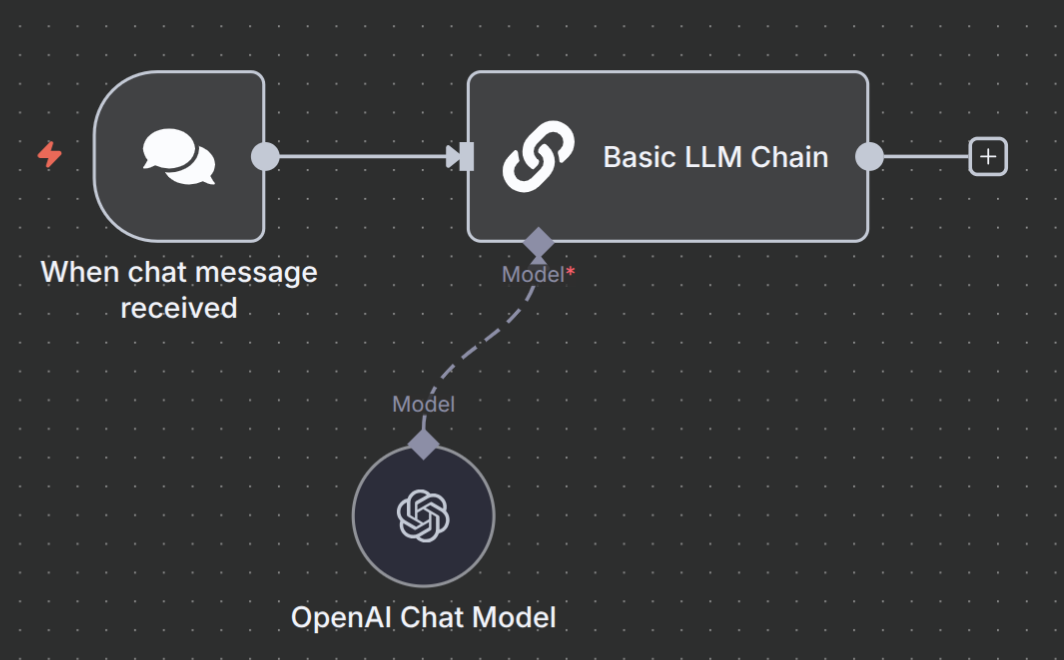
\includegraphics[width=0.8\textwidth]{slike/04/Base LLM.png}
    \caption{AI асистент у \textit{n8n}}
    \label{fig:04-7}
\end{figure}


\subsubsection*{Ниво 2: RAG Системи (Retrieval-Augmented Generation)}

Једно од кључних ограничења великих језичких модела (LLM) јесте чињеница да је њихово знање
замрзнуто у тренутку тренирања и да не обухвата специфичне, интерне или ажуриране информације
организације у којој се користе. Поред тога, LLM модели су склони тзв. халуцинацијама – генерисању
уверених, али нетачних одговора када немају довољно поуздан контекст.
Како би се ови проблеми превазишли, развијена је архитектура RAG (енг. \textit{Retrieval-Augmented Generation})~\cite{lewis2020rag,gao2024ragsurvey},
која комбинује предности класичних система за претрагу информација и генеративних AI модела.
Уместо да се LLM посматра као свеобухватна „енциклопедија“, RAG га трансформише у
процесор информација који активно користи спољне изворе знања у реалном времену.
У овом приступу, модел више не одговара искључиво на основу параметара научених током тренирања,
већ генерише одговор на основу \textit{relevantnog konteksta} који му се динамички доставља
из интерне базе знања организације.
RAG системи се фундаментално разликују од класичних претраживача заснованих на кључним речима
(\textit{keyword search}). Уместо тражења дословног поклапања термина,
RAG користи семантичку претрагу, која се заснива на значењу текста, а не на његовој форми.
На тај начин, систем може пронаћи релевантне информације чак и када се формулација питања
разликује од формулације у документима. Пример RAG система дат је на слици~\ref{fig:04-8}

\begin{figure}[h!]
    \centering
    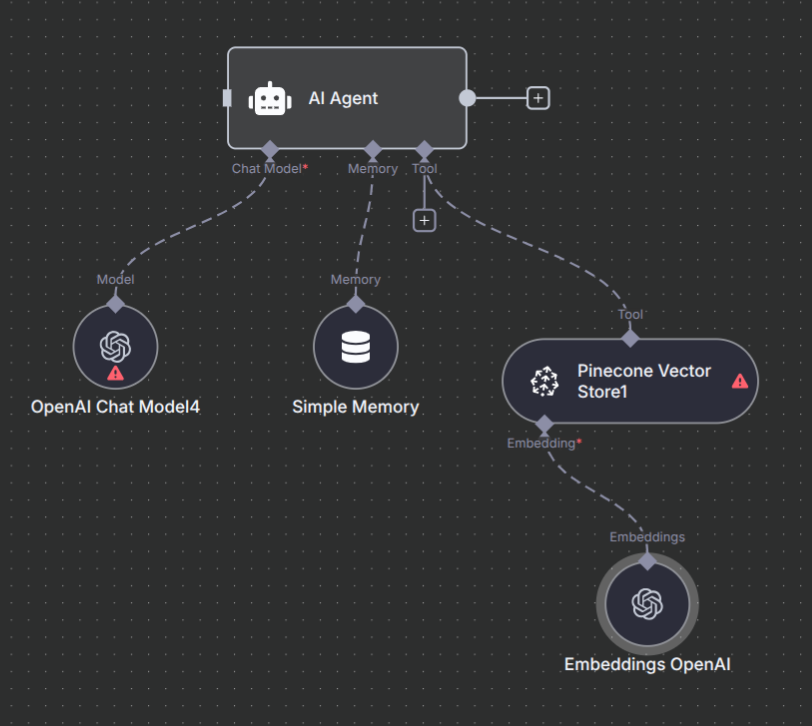
\includegraphics[width=0.7\textwidth]{slike/04/RAG.png}
    \caption{RAG у \textit{n8n}}
    \label{fig:04-8}
\end{figure}

Техничка архитектура RAG-а састоји се од неколико јасно раздвојених фаза:

\begin{enumerate}
    \item \textbf{Ingestion (Унос и припрема података):} \\
    Документи организације (PDF, Word, HTML, базе знања, вики странице) пролазе кроз процес обраде
    током којег се чисте, нормализују и деле на мање, логички смислене целине
    (енг. \textit{chunks}). Ова подела је кључна, јер превелики делови умањују прецизност претраге,
    док превише мали делови губе контекст.

    \item \textbf{Embedding (Векторизација значења):} \\
    Сваки сегмент текста се трансформише у нумеричку репрезентацију – вектор –
    коришћењем embedding модела~\cite{mikolov2013,reimers2019sbert}. Овај вектор кодира семантичко значење текста,
    тако да слични појмови и реченице имају сличне векторске репрезентације.
    Добијени вектори се складиште у специјализованој векторској бази података
    (нпр. Pinecone, Qdrant, Weaviate), оптимизованој за брзу семантичку претрагу~\cite{johnson2019faiss}.

    \item \textbf{Retrieval (Семантичка претрага):} \\
    Када корисник постави питање, и оно се преводи у векторски облик користећи исти embedding модел.
    Систем затим проналази оне сегменте из базе чији су вектори математички
    „најближи“ вектору питања, најчешће коришћењем косинусне сличности или сличних метрика~\cite{karpukhin2020dpr}.
    Резултат ове фазе није један документ, већ скуп најрелевантнијих контекстуалних исечака.

    \item \textbf{Synthesis (Контекстуална синтеза и генерисање):} \\
    Пронађени текстуални сегменти се затим комбинују са оригиналним корисничким питањем
    и прослеђују LLM моделу као додатни контекст у промпту.
    На основу тог контекста, модел генерише одговор који је директно утемељен
    у доступним документима, уместо у општем, генеричком знању.
\end{enumerate}

\begin{tcolorbox}[colback=yellow!10!white,colframe=orange!75!black,title=Prednost RAG-a: Utemeljenje (Grounding)]
Кључна предност RAG архитектуре јесте утемељење одговора у проверљивим изворима.
Уместо генеричких или спекулативних одговора, систем може експлицитно да се позове
на конкретан документ или део интерне документације, на пример:
\textit{„Према интерном правилнику, поглавље 3.2, процедура је следећа...“}.
У ситуацијама када релевантна информација не постоји у бази знања,
добро дизајниран RAG систем преферира одговор типа \textit{„Ta informacija nije dostupna“},
чиме се значајно смањује ризик од халуцинација и погрешних пословних одлука.


\end{tcolorbox}

\subsubsection*{Ниво 3: AI Агенти (Аутономни Системи)}

Док RAG архитектура проширује способности великих језичких модела додавањем
приступа екстерним изворима знања (метафорички, даје им „очи“),
AI агенти представљају следећи еволутивни корак: они систему додају „руке“,
односно способност да активно делује у окружењу.
Увођење агената означава прелаз са пасивних система, који искључиво генеришу
текстуалне одговоре, на аутономне системе за решавање проблема.
Такви системи не само да разумеју захтев корисника,
већ су у стању да самостално планирају, извршавају и прилагођавају низ акција
како би задати циљ био постигнут.

У контексту вештачке интелигенције, појам примене агената (енг. \textit{agency})
односи се на способност система да:
\begin{itemize}
    \item самостално интерпретира циљ,
    \item доноси одлуке о наредним корацима,
    \item извршава акције у окружењу,
    \item прилагођава понашање на основу повратних информација.
\end{itemize}

AI агент се, стога, дефинише као софтверски ентитет који аутономно
формира секвенцу акција неопходних за постизање задатог циља,
без потребе да сваки појединачни корак буде унапред експлицитно дефинисан од стране инжењера.
Ово представља кључну разлику у односу на традиционалну аутоматизацију.
Код класичних workflow система, сваки корак је унапред „закуцан“ у логику процеса.
Код агената, инжењер дефинише \textbf{шта} је циљ,
док агент самостално одлучује \textbf{како} ће до тог циља доћи.

Доминантна парадигма за имплементацију савремених AI агената данас је образац
\textbf{ReAct} (енг. \textit{Reasoning + Acting})~\cite{yao2022react,wang2024agents}.
Овај образац уводи цикличну структуру размишљања и деловања,
чиме се превазилази ограничење линеарних токова обраде.
Уместо да генерише комплетан одговор „у једном пролазу“,
агент функционише као систем са повратном спрегом,
континуирано прилагођавајући своје понашање на основу резултата претходних акција.

ReAct петља се састоји од три основне фазе:

\begin{enumerate}
    \item \textbf{Thought (Размишљање):} \\
    Агент анализира тренутно стање система, интерпретира кориснички захтев
    и доноси одлуку о следећем кораку.
    Овај корак представља интерни процес резоновања и планирања.

    \item \textbf{Action (Акција):} \\
    На основу донете одлуке, агент бира одговарајући алат
    (API позив, функцију, базу података, спољашњи сервис)
    и генерише конкретне параметре за његово извршавање.

    \item \textbf{Observation (Опсервација):} \\
    Резултат извршене акције се враћа агенту као нова информација.
    Овај резултат може бити податак, порука о успеху или грешка,
    и директно утиче на следећи циклус размишљања.
\end{enumerate}

Ова итеративна структура омогућава агенту да учи из сопствених акција
и динамички прилагођава стратегију извршавања. На овај начин агент у потпуности опонаша начине на који људи делују током решавања било ког проблема генерално.

\paragraph*{Пример извршења ReAct петље}

Размотримо кориснички захтев:
\textit{„Провери цену акција компаније Apple, конвертуј то у евре и пошаљи ми на Slack.“}

\begin{tcolorbox}[colback=white,colframe=black,title=Unutrašnji proces agenta]
\textbf{Итерација 1:}
\begin{itemize}
    \item \textit{Thought:} Потребна ми је тренутна цена акција Apple-а (AAPL).
    Тај податак није део мог статичког знања.
    \item \textit{Action:} \texttt{get\_stock\_price(symbol="AAPL")}
    \item \textit{Observation:} 185.50 USD
\end{itemize}

\textbf{Итерација 2:}
\begin{itemize}
    \item \textit{Thought:} Цена је у доларима, али корисник жели износ у еврима.
    \item \textit{Action:} \texttt{currency\_converter(from="USD", to="EUR", amount=185.50)}
    \item \textit{Observation:} 170.25 EUR
\end{itemize}

\textbf{Итерација 3:}
\begin{itemize}
    \item \textit{Thought:} Имам коначан резултат, потребно је обавестити корисника.
    \item \textit{Action:} \texttt{send\_slack\_message(channel="general", text="Cena AAPL je 170.25 EUR")}
    \item \textit{Observation:} Success: Message sent.
\end{itemize}

\textbf{Final Answer:} Задатак је успешно обављен.
\end{tcolorbox}
\noindent
Овај пример илуструје способност агента да повезује излаз једне акције
са улазом следеће (\textit{chaining}),
што је фундаментално различито од понашања класичних chatbot система.

\paragraph*{Техничка реализација: Tool Calling (Function Calling)}

Важно је нагласити да LLM модели сами по себи немају могућност извршавања кода
или интеракције са спољним системима.
Они функционишу искључиво као напредни процесори текста.
Да би агент могао да делује у реалном свету,
користи се механизам познат као \textit{Tool Calling} или \textit{Function Calling}~\cite{schick2023toolformer},
који омогућава да модел изабере одговарајући алат
и генерише структурирани захтев за његово извршење.

Доступни алати се агенту експлицитно описују приликом иницијализације,
најчешће кроз формалну спецификацију у облику \textbf{JSON Schema}~\cite{openai2024toolcalling,patil2023gorilla}.
Ова спецификација дефинише:
\begin{itemize}
    \item назив алата,
    \item опис његове намене,
    \item параметре које прихвата и њихове типове.
\end{itemize}

\begin{lstlisting}[language=json, caption={Definicija alata koju agent "vidi"}]
{
  "name": "get_weather",
  "description": "Dohvata trenutnu temperaturu za dati grad",
  "parameters": {
    "type": "object",
    "properties": {
      "city": {"type": "string", "description": "Ime grada"},
      "unit": {"type": "string", "enum": ["celsius", "fahrenheit"]}
    },
    "required": ["city"]
  }
}
\end{lstlisting}

На основу корисничког захтева,
модел не генерише слободан текстуални одговор,
већ структурирани позив алата са одговарајућим аргументима.
Рунтиме окружење затим извршава стварну функцију
и враћа резултат моделу као нови улаз за даљу обраду.

\paragraph*{Меморија и планирање}

Да би AI агент био заиста аутономан и способан за дуготрајно, смислено деловање,
мора поседовати механизме за памћење стања и планирање акција.
Без ових компоненти, систем се своди на простог извршиоца појединачних API позива,
без разумевања контекста, континуитета и циљне структуре задатка.
Меморија омогућава агенту да задржи информације о претходним корацима,
док планирање омогућава да те информације користи за доношење одлука
које нису локално оптималне, већ су усмерене ка остваривању крајњег циља.

Меморија агента не представља само историју порука,
већ структурисано управљање стањем система.
У пракси се разликују најмање два нивоа меморије:

\begin{itemize}
    \item \textbf{Краткорочна меморија (радна меморија):} \\
    Овај тип меморије обухвата контекст тренутне сесије и
    укључује резултате претходних акција, привремене варијабле,
    међурезултате и одлуке донете у току извршавања задатка. Величину и расположивост овог контекста директно ограничава \textit{context window} модела, при чему пракса показује да модели често „губе“ информације смештене у средини дугачких улаза~\cite{liu2023lostmiddle}.
    Краткорочна меморија се обично чува у оквиру рунтиме окружења
    (нпр. у меморији процеса или у оквиру контекста workflow-а)
    и брише се по завршетку задатка.

    \item \textbf{Дугорочна меморија (трајна меморија):} \\
    Дугорочна меморија омогућава агенту да задржи знање између различитих сесија
    и интеракција. Она се најчешће имплементира коришћењем
    векторских база података, које омогућавају семантичко складиштење
    и претрагу информација. На овај начин, агент може „памтити“:
    \begin{itemize}
        \item преференце и навике корисника,
        \item претходно решене проблеме и њихове исходе,
        \item интерне процедуре, документацију и правила,
        \item сопствена искуства из ранијих извршавања.
    \end{itemize}
\end{itemize}
\noindent
Важно је нагласити да дугорочна меморија не функционише као класична база чињеница,
већ као асоцијативни систем заснован на значењу, што омогућава флексибилно
призивање релевантних информација у различитим контекстима.

Поред меморије, кључна компонента аутономије јесте способност планирања.
Уместо да реагује искључиво на наредни корак,
агент је у стању да сагледа циљ у целини
и разложи га на низ међусобно зависних под-задатака.

За ову сврху се користе технике резоновања попут:
\begin{itemize}
    \item \textit{Chain of Thought} – експлицитно размишљање кроз кораке~\cite{wei2022cot},
    \item \textit{Self-Consistency} – узорковање више путања и избор најконзистентнијег закључка~\cite{wang2022selfconsistency},
    \item \textit{Tree of Thoughts} – гранање и евалуација више путања резоновања~\cite{yao2023tot},
    \item хијерархијско планирање – разлагање циља на фазе и активности,
    \item итеративно репланирање – прилагођавање плана током извршавања~\cite{shinn2023reflexion,madaan2023selfrefine}.
\end{itemize}

На пример, за задатак \textit{„Направи анализу тржишта“},
агент може прво формирати апстрактан план
(прикупљање података, анализа, синтеза),
а затим сваку фазу додатно разложити на конкретне акције
(претрага извора, екстракција података, поређење цена, генерисање извештаја).

\paragraph*{Само-корекција и учење из грешака}

Једна од најважнијих особина аутономних агената јесте способност
\textbf{само-корекције}.
У овом моделу, грешке се не посматрају као фатални проблеми,
већ као нова информација у процесу резоновања.

Ако нека акција не успе (нпр. API врати грешку, ресурс није доступан,
или резултат не задовољава очекивања),
агент ту информацију прима кроз фазу опсервације
и користи је за прилагођавање наредних корака.
То може укључивати промену алата, модификацију параметара
или редефинисање плана.

Ова отпорност на грешке (\textit{resilience})
омогућава агентима да функционишу у реалним,
динамичким и непредвидивим окружењима,
где потпуна контрола над спољним системима није могућа.
Пример једноставног AI система  за слање мотивационих порука дат је на слици~\ref{fig:04-9}. LLM се користи искључиво за генерисање текста, док су извори података и акције слања
реализовани кроз детерминистичке n8n чворове.

\begin{figure}[h!]
    \centering
    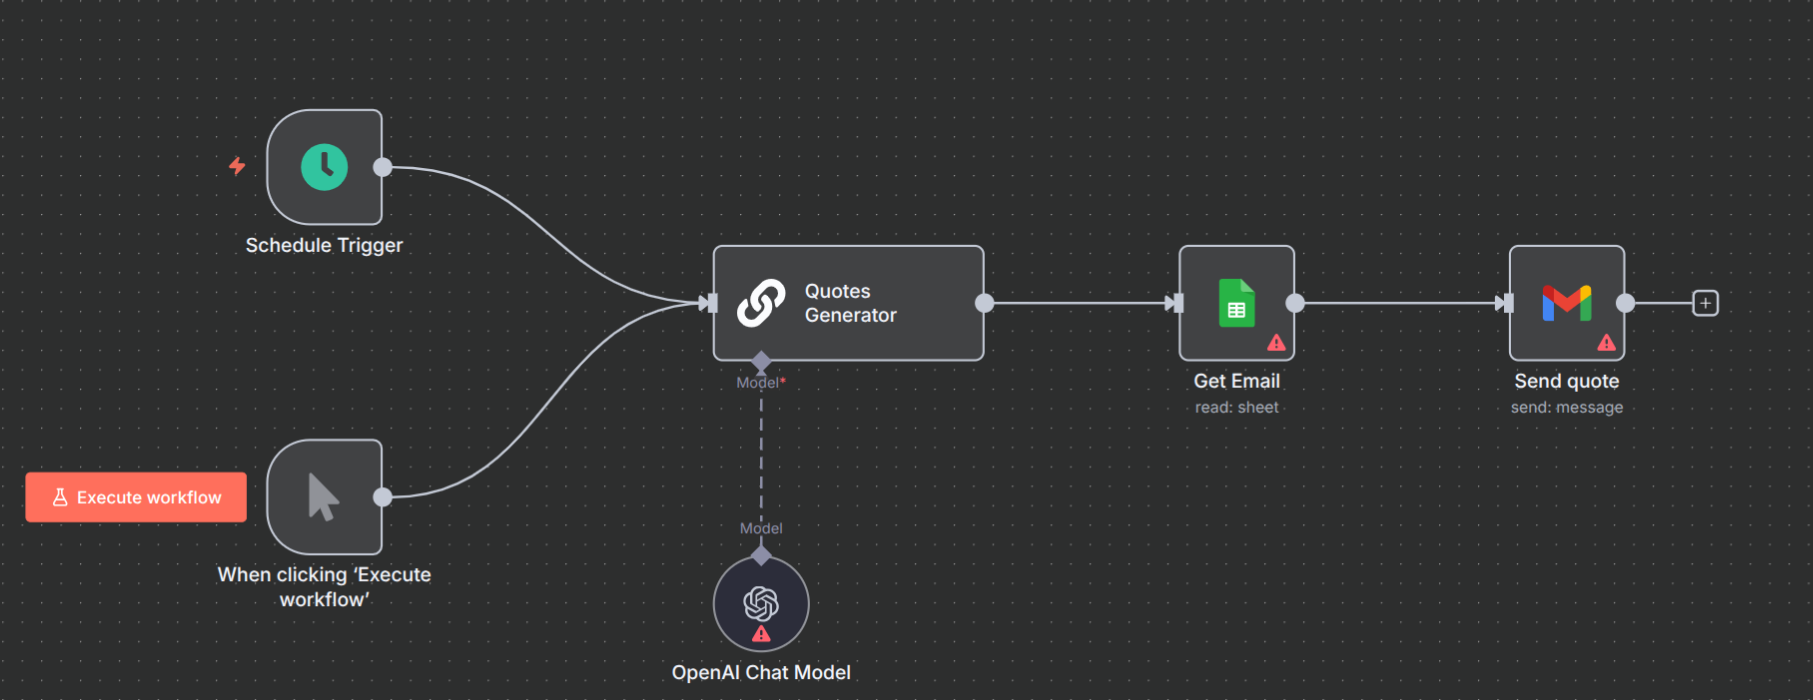
\includegraphics[width=0.85\textwidth]{slike/04/primer_agenta_quote.png}
    \caption{Агент за генерисање мотивационих порука у \textit{n8n}}
    \label{fig:04-9}
\end{figure}

% =================================================================================
% POGLAVLJE 3.4 - PROŠIRENA VERZIJA
% =================================================================================

\subsection{Ниво 4: Мулти-Агентски Системи (MAS)}

Док појединачни агенти представљају моћне алате, они поседују инхерентна ограничења када се суоче са задацима високе комплексности.
Један агент опремљен са десет различитих алата и дугачким системским промптом често постаје "збуњен" – губи фокус, халуцинира инструкције или неисправно бира алате. Ово је познато као проблем "уског грла контекста" (енг. \textit{Context Bottleneck}).
Решење лежи у Мулти-Агентским Системима (MAS)~\cite{wu2023autogen,park2023agents,li2023camel}. Ови системи симулирају организациону структуру људских тимова, где се комплексан проблем разбија на мање целине које решавају специјализовани, колаборативни агенти.

Кључна предност MAS архитектуре је модуларност. Уместо једног генералног агента ("Jack of all trades"), креира се тим експерата:
\begin{itemize}
    \item Сваки агент има свој, високо специфичан системски промпт (нпр. "Ти си сениор Python инжењер...").
    \item Сваки агент има приступ само оним алатима који су му неопходни (смањује ризик од грешке).
    \item Агенти могу користити различите LLM моделе (нпр. јефтинији модел за сумирање, скупљи и паметнији модел за решавање логике).
\end{itemize}

У зависности од природе проблема, инжењери бирају различите топологије сарадње између агената. Три најдоминантнија обрасца су:

\paragraph*{1. Хијерархијска сарадња (Supervisor / Router Pattern)}
Овај образац имитира корпоративну структуру "Менаџер - Запослени".

\begin{itemize}
    \item \textbf{Супервизор (Router):} Централни чвор система. Овај агент обично користи напредан модел (нпр. GPT-4o). Он не извршава задатке директно. Његова улога је да анализира захтев корисника, разбије га на под-задатке и одлучи којем раднику да делегира посао. Такође, он врши инспекцију резултата пре него што их врати кориснику.
    \item \textbf{Радници (Workers):} Специјализовани агенти који оперишу у изолацији.
\end{itemize}

\textbf{Пример тока података:}
\begin{enumerate}
    \item Корисник: „Напиши ми код за Snake игрицу у Python-у и генериши слику за лого.“
    \item Супервизор анализира и каже: „За кодирање зовем \textit{DevAgent}, за лого зовем \textit{DesignAgent}.“
    \item \textit{DevAgent} пише код и враћа га Супервизору.
    \item \textit{DesignAgent} црта слику и враћа је Супервизору.
    \item Супервизор спаја оба резултата и шаље финални одговор кориснику.
\end{enumerate}

\paragraph*{2. Секвенцијална сарадња (енг. \textit{The Assembly Line)}}
Овај образац функционише као производна трака. Излаз једног агента постаје директан улаз за следећег агента. Овде не постоји централни менаџер који одлучује – путања је унапред дефинисана (\textit{Hard-coded workflow}).

Ово је идеално за процесе који имају стриктан редослед.

\textbf{Пример: Креирање Блога}
\begin{itemize}
    \item \textbf{Агент 1 (Истраживач):} Претражује Google на задату тему и креира сирови сажетак чињеница. $\rightarrow$ Прослеђује текст.
    \item \textbf{Агент 2 (Писац):} Узима чињенице и пише ангажован чланак пратећи SEO правила. $\rightarrow$ Прослеђује нацрт.
    \item \textbf{Агент 3 (Уредник):} Чита нацрт, исправља граматичке грешке и проверава тон комуникације. $\rightarrow$ Финални текст.
\end{itemize}

Предност овог приступа је предвидљивост и лакоћа дебаговања, јер је сваки корак јасно раздвојен.

\paragraph*{3. Колаборативна дебата (енг. \textit{Joint Collaboration / Network)}}
Ово је најкомплекснији, али и најмоћнији облик сарадње, инспирисан академским или инжењерским "brainstorming" сесијама. Агенти нису пасивни извршиоци, већ активно комуницирају једни са другима у петљи, критикују туђи рад и предлажу побољшања.

У овом моделу често се уводи улога Критичара (Critique Agent).

\textbf{Пример: Развој Софтвера}
\begin{itemize}
    \item \textbf{Coder Agent:} Пише иницијалну верзију кода~\cite{chen2021codex}.
    \item \textbf{Reviewer Agent:} Анализира тај код. Не извршава га, већ тражи сигурносне пропусте (бугове). Враћа feedback: "Линија 42 је несигурна, може доћи до SQL Injection напада."
    \item \textbf{Coder Agent:} Прима критику, размишља („Thought: У праву је, морам да санитизујем input“) и пише верзију 2.0.
    \item Процес се понавља док Reviewer Agent не каже "Одобрено"~\cite{wang2023voyager}.
\end{itemize}
\noindent
Овај итеративни процес доказано повећава квалитет излазног резултата у односу на "Single-shot" генерисање (где модел има само једну шансу да погоди решење).

\paragraph*{Управљање стањем (Shared State)}

Једно од најважнијих техничких питања у дизајну мулти-агентских система јесте:
\textit{Како агенти деле информације и како се обезбеђује конзистентност њиховог рада?}
За разлику од single-agent система, где је ток размишљања и акција садржан у једној инстанци,
мулти-агентски системи захтевају експлицитан механизам за размену контекста.
Без јасно дефинисаног заједничког стања, агенти би радили изоловано, што би довело до
дуплирања рада, контрадикторних одлука или губитка информација.

У савременим оквирима за изградњу MAS-а (као што су LangGraph или AutoGen),
овај проблем се решава увођењем концепта \textbf{Дељеног Стања} (\textit{Shared State} или \textit{Graph State}).
Дељено стање представља централни, структурирани објекат који садржи све релевантне информације
о тренутном статусу задатка и који се прослеђује између агената током извршавања система.

Технички, дељено стање је најчешће имплементирано као JSON објекат који обухвата:
\begin{itemize}
    \item оригинални захтев корисника,
    \item парцијалне резултате рада појединачних агената,
    \item мета-информације о томе који кораци су завршени,
    \item повратне информације (feedback) и одлуке надређених агената,
    \item сигнализацију да ли је задатак завршен или захтева додатну обраду.
\end{itemize}

\begin{lstlisting}[language=json, caption={Primer deljenog stanja u multi-agentskom sistemu}]
{
  "user_request": "Napravi izveštaj o prodaji",
  "data_gathered": true,
  "raw_data": [ ... ],
  "draft_report": "Prodaja je porasla za 20%...",
  "manager_approval": false,
  "feedback": "Dodaj grafikone u sekciju 3"
}
\end{lstlisting}

Сваки агент у систему добија приступ овом стању као улаз.
На основу свог системског промпта и улоге, агент:
\begin{enumerate}
    \item чита релевантне делове стања,
    \item извршава своју специфичну одговорност,
    \item ажурира стање новим информацијама или одлукама,
    \item прослеђује ажурирано стање следећем агенту или назад супервизору.
\end{enumerate}

На пример, аналитички агент може да попуни поље \texttt{raw\_data},
писац извештаја генерише \texttt{draft\_report},
док супервизорски агент мења вредност \texttt{manager\_approval} у \texttt{true}
када процени да је резултат прихватљив.

Овакав приступ има неколико кључних предности:
\begin{itemize}
    \item омогућава \textbf{транспарентност} процеса — јасно је у којој фази се задатак налази,
    \item олакшава \textbf{debugging и аудит} јер се свака одлука рефлектује у стању,
    \item омогућава \textbf{паралелни рад} агената над различитим деловима истог проблема,
    \item спречава неконтролисано „размишљање“ модела ван дефинисаног контекста.
\end{itemize}

Истовремено, дељено стање намеће и строгу дисциплину у дизајну система:
што је стање комплексније и неструктурисаније, већи је ризик од грешака,
неконзистентности и неочекиваних понашања агената.
Због тога се у пракси често уводе формалне шеме (\textit{schemas}) и валидација стања,
како би се осигурало да сваки агент види и мења само оне делове стања за које је задужен. 

На слици~\ref{fig:04-10} дат је пример мулит-агентског система у \textit{n8n}. Улазни захтеви се нормализују и прослеђују супервизорском агенту, који на основу садржаја
делегира задатке специјализованим агентима (е-маил, истраживање, управљање задацима, календар).
Сваки агент користи велики језички модел искључиво за разумевање захтева, док се стварне
акције извршавају кроз детерминистичке API позиве.

\subsubsection{Компаративна анализа система}

Табела~\ref{tab:04-2} приказује компаративни преглед кључних функционалних способности четири доминантне категорије савремених AI система: класичних AI асистената заснованих на великим језичким моделима (LLM), RAG система (Retrieval-Augmented Generation), аутономних AI агената и мулти-агентских система (MAS).

\textbf{AI асистенти} представљају најосновнији облик интеракције са великим језичким моделима. Њихова функционалност се своди на генерисање одговора на основу корисничког упита, без експлицитне везе са спољним изворима знања или могућности извршавања акција. Овакви системи су у потпуности реактивни: не поседују сопствену иницијативу, не памте стање између интеракција и не могу доносити одлуке ван граница једног промпт–одговор циклуса. Због тога су погодни за опште информативне задатке, објашњења и креативно генерисање садржаја, али нису адекватни за комплексне пословне или оперативне процесе.

\textbf{RAG системи} представљају значајан корак напред у односу на чисте AI асистенте. Увођењем семантичке претраге над екстерним документима (путем embedding-а и векторских база), RAG омогућава утемељење генерисаних одговора у конкретним изворима знања. Ипак, иако RAG системи поседују дугорочну меморију у виду документационог репозиторијума, они су и даље фундаментално пасивни. Њихова улога је ограничена на побољшано одговарање на упите, без способности планирања, извршавања акција или управљања сложеним токовима рада.

\textbf{AI агенти} уводе концепт аутономије и оперативне интелигенције. За разлику од асистента и RAG система, агенти су дизајнирани да раде у итеративној петљи \textit{Thought–Action–Observation}, при чему могу самостално доносити одлуке, позивати спољне алате (API-је, базе података, скрипте), анализирати резултате и прилагођавати даље кораке. Кључна разлика је у томе што агент поседује унутрашње стање (сессион мемори), способност планирања и механизме само-корекције. Тиме агент прелази из пасивне у активну улогу, где може извршавати задатке од почетка до краја уз минималну људску интервенцију.

\textbf{Мулти-агентски системи (MAS)} представљају најнапреднији облик агентске архитектуре. Они су неопходни у сценаријима где задаци нису линеарни, већ захтевају паралелну обраду, специјализацију и координацију више аутономних ентитета. Уместо једног универзалног агента, MAS се састоји од више агената са јасно дефинисаним улогама (нпр. истраживач, планер, извршилац, евалуатор). Сваки агент је оптимизован за своју функцију путем посебног промпта, алата и ограничења, док централни оркестрациони механизам управља разменом информација и делегирањем задатака.

Кључна предност мулти-агентских система лежи у њиховој способности да решавају комплексне, нелинеарне проблеме на дистрибуиран начин. Паралелизација рада, хијерархијско планирање и међусобна евалуација агената доводе до веће робусности, тачности и скалабилности система. Због тога се MAS архитектуре све чешће примењују у напредним пословним аутоматизацијама, истраживачким платформама, аутономним аналитичким системима и сложеним организационим процесима.

Сумарно, табела~\ref{tab:04-2} јасно показује да разлика између наведених система није само у количини функционалности, већ у њиховој епистемолошкој и оперативној улози. Док AI асистенти и RAG системи служе као алати за подршку кориснику, AI агенти и посебно мулти-агентски системи представљају самосталне извршне ентитете, способне да преузму активну улогу у доношењу одлука и реализацији комплексних задатака.

\begin{small}
\begin{longtable}{|p{5.2cm}|c|c|c|c|}
\caption{Матрица способности: Chatbot vs RAG vs AI Агент vs Мулти-Агент систем}\label{tab:04-2}\\
\hline
\textbf{Способност / карактеристика}
& \textbf{AI Асистент (LLM)}
& \textbf{RAG}
& \textbf{AI Агент}
& \textbf{Мулти-Агент} \\
\hline
\endfirsthead
\hline
\textbf{Способност / карактеристика}
& \textbf{AI Асистент (LLM)}
& \textbf{RAG}
& \textbf{AI Агент}
& \textbf{Мулти-Агент} \\
\hline
\endhead
\hline
\endfoot

Одговарање на питања / генерисање текста & Х & Х & Х & Х \\
\hline
Утемељење у екстерним документима (grounding) &  & Х & Х & Х \\
\hline
Семантичка претрага (embedding + вектор база) &  & Х & Х & Х \\
\hline
Структурисан излаз (JSON схема / валидација) &  &  & Х & Х \\
\hline
Извршавање акција (tool/function calling) &  &  & Х & Х \\
\hline
Итеративна петља (ReAct: Thought--Action--Observation) &  &  & Х & Х \\
\hline
Краткорочна меморија стања (session state) &  &  & Х & Х \\
\hline
Дугорочна меморија између сесија (persistent memory) &  & Х & Х & Х \\
\hline
Планирање и декомпозиција задатака &  &  & Х & Х \\
\hline
Само-корекција и репланирање након грешке &  &  & Х & Х \\
\hline
Специјализација улога (нпр. Researcher, Executor, Critic) &  &  &  & Х \\
\hline
Делегирање и координација (task routing између агената) &  &  &  & Х \\
\hline
Паралелизација рада (истовремени суб-таскови) &  &  &  & Х \\
\hline
Централна контрола и guardrails на нивоу организације &  & Х & Х & Х \\
\hline
Observability: логови/метрике/tracing по корацима &  & Х & Х & Х \\
\hline
\end{longtable}
\end{small}


\begin{figure}[h!]
    \centering
    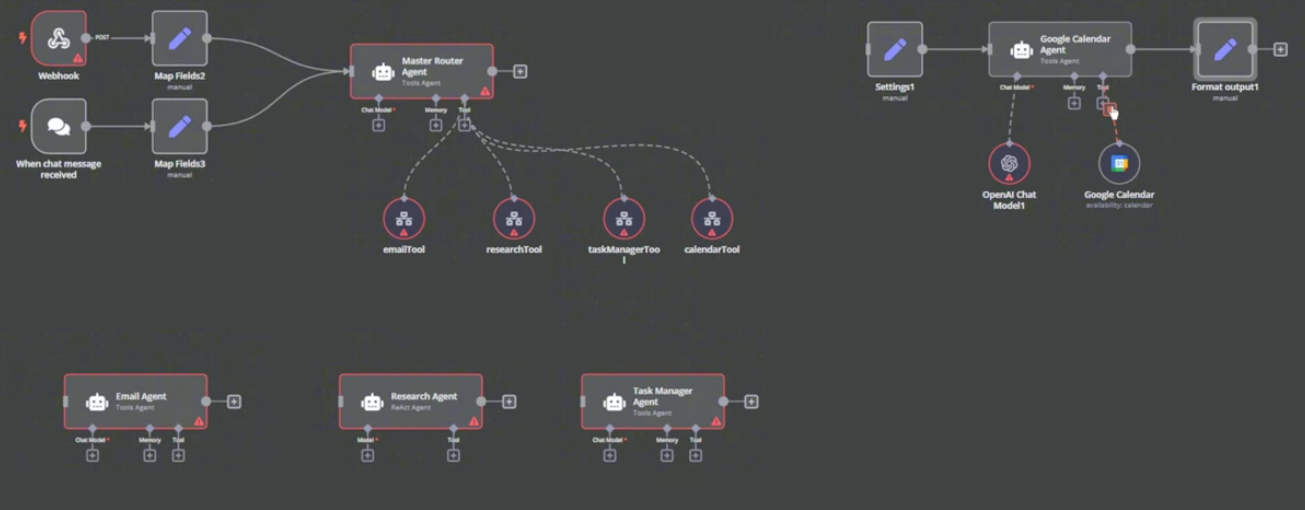
\includegraphics[width=0.95\textwidth]{slike/04/multiagent.png}
    \caption{Мултиагентски систем у \textit{n8n}}
    \label{fig:04-10}
\end{figure}


\newpage

% =================================================================================
% POGLAVLJE: VELIKI JEZIČKI MODELI (LLM)
% =================================================================================

% =================================================================================
% POGLAVLJE: VELIKI JEZIČKI MODELI - AKADEMSKA VERZIJA
% =================================================================================

\section{Велики Језички Модели: Когнитивни мотор система}

У основи савремених система за аутоматизацију, од једноставних процесора текста до комплексних мулти-агентских архитектура, налази се технологија великих језичких модела (енг. \textit{Large Language Models - LLM}).

За успешно пројектовање аутоматизованих система у алатима као што је \textit{n8n}, императив је превазићи површно разумевање LLM-а као „напредног chatbot-а“. Инжењерски приступ захтева дубинско познавање архитектуре, ограничења и пробабилистичке природе ових модела. Разумевање интерне логике модела омогућава предвиђање понашања система, оптимизацију потрошње ресурса (токена) и имплементацију механизама за контролу грешака.

\subsection{Дефиниција и декомпозиција појма LLM}

Велики језички модел се дефинише као напредни систем вештачке интелигенције, заснован на архитектури дубоких неуронских мрежа (примарно \textit{Transformer} архитектури)~\cite{vaswani2017,goodfellow2016}, који је способан да разуме, генерише и манипулише симболичким системима, укључујући природне језике и програмске кодове~\cite{devlin2019,brown2020}.

Водећи модели на тржишту, као што су GPT-4.1 (OpenAI)~\cite{openai2023gpt4,bubeck2023}, Claude 4.5 (Anthropic)~\cite{anthropic2024claude} и DeepSeek v3.2, представљају врхунац ове технологије. Отворена алтернатива, као што је LLaMA породица модела~\cite{touvron2023}, као и Mistral~\cite{jiang2023mistral}, BLOOM~\cite{bigscience2022bloom} и PaLM~\cite{chowdhery2022palm}, такође је допринела ширем екосистему истраживачких и комерцијалних модела. Да би се разумела њихова комплексност, неопходно је анализирати три компоненте њиховог назива:

\paragraph{Велики (Large)}
Атрибут "Велики" односи се на две кључне димензије скалабилности:
\begin{itemize}
    \item \textbf{Обим података за тренинг:} Ови модели се тренирају на корпусима података који се мере у петабајтима, обухватајући значајан део јавно доступног интернета (Common Crawl), милионе дигитализованих књига, научних радова и репозиторијума кода.
    \item \textbf{Број параметара:} Параметри представљају интерне променљиве (тежине веза у неуронској мрежи) које модел подешава током процеса учења. Савремени модели поседују од неколико милијарди (7Б) до преко билион (1Т+) параметара~\cite{kaplan2020scaling,fedus2022switch,hoffmann2022chinchilla}. Број параметара директно корелира са способношћу модела да апстрахује комплексне концепте и нијансе у расуђивању~\cite{wei2022emergent,hendrycks2021mmlu}.
\end{itemize}

\paragraph{Језички (Language)}
Иако се називају "језичким", ови модели суштински оперишу над симболима (реч, број, знак). У контексту LLM-а, језик се не односи само на лингвистичке системе (српски, енглески), већ на било који систем симбола са дефинисаном синтаксом и семантиком. То укључује програмске језике (Python, JavaScript), формате података (JSON, XML) и математичку нотацију. Модел учи мапирање и односе између ових симбола, што му омогућава "превођење" природног захтева у извршни код.

\paragraph{Модел (Модел)}
Ово је концептуално најважнија дистинкција. LLM није база података, нити енциклопедија. Он је \textbf{статистичка репрезентација} података на којима је трениран. Он не "складишти" информације у класичном смислу (као фајлове), већ моделује вероватноћу појављивања одређених секвенци симбола у одређеном контексту.

\subsection{Епистемолошка природа LLM-а: Компресија са губитком}

У популарним објашњењима, велики језички модели (LLM) се често описују као
„библиотека свих књига“ или „дигитални енциклопедијски ум“.
Иако је ова аналогија интуитивна, она је технички и епистемолошки непрецизна,
јер имплицира да модел поседује експлицитно складиштене чињенице и да
приликом одговарања врши процес \textit{претраге и проналажења} информација
(\textit{retrieval}).

Прецизнија инжењерска аналогија гласи:
\textbf{LLM представља екстремно компресовану репрезентацију великог дела јавно доступног
људског знања, изведену кроз процес компресије са губитком}
(\textit{lossy compression})~\cite{bender2021,zhao2023llmsurvey}.
Ова перспектива је кључна за разумевање како LLM модели „знају“,
али и зашто понекад греше на систематичан и предвидив начин.

Код класичних алгоритама за компресију података са губитком,
попут JPEG-а за слике или MP3-а за звук,
оригинални сигнал се не чува у потпуности.
Уместо тога, алгоритам идентификује статистичке обрасце
и уклања детаље који се сматрају мање важним за перцепцију.
На пример, JPEG алгоритам не памти вредност сваког појединачног пиксела,
већ апроксимира слику кроз фреквенцијске компоненте,
чувајући глобалне структуре, ивице и боје,
док се ситни детаљи жртвују ради смањења величине фајла.
Аналогно томе, LLM модели не памте појединачне реченице,
документе или чињенице из тренинг података.
Уместо тога, током тренирања они уче
статистичке обрасце у језику:
како се појмови повезују, које речи типично следе једна другу,
какве структуре имају објашњења, дефиниције и аргументи.
Резултат овог процеса није база знања,
већ параметарски модел (милијарде или трилиони тежина)
који представља компресовану мапу вероватноћа над језиком.

Много конфузије уноси чињеница да општа јавност најчешће поистовећује LLM са базом података, међутим разлика између истих је очигледна.
Ова разлика се може јасно илустровати поређењем класичних база података
и великих језичких модела:

\begin{itemize}
    \item \textbf{База података} функционише по принципу
    \textit{lookup} операције.
    Ако се затражи податак који постоји у бази,
    систем враћа тачно онај запис који је претходно уписан.
    Тачност је детерминистичка, а грешка углавном указује на
    непостојање или погрешан унос података.

    \item \textbf{LLM} функционише по принципу
    \textit{rekonstrukcije}.
    Када се моделу постави питање,
    он не претражује меморију у потрази за „тачним одговором“,
    већ генерише одговор токен по токен,
    на основу вероватноћа научених током тренирања.
    Другим речима, одговор се реконструише,
    а не проналази.
\end{itemize}
\noindent
Ова реконструктивна природа објашњава зашто LLM модели могу
давати изузетно флуентне и уверљиве одговоре чак и у ситуацијама
када немају експлицитно знање о траженој чињеници. 

\subsubsection*{Знање као дистрибуција, а не као чињеница}

Епистемолошки посматрано,
знање у LLM-у није скуп истинитих тврдњи,
већ \textbf{дистрибуција вероватноћа над могућим исказима}.
Модел „зна“ да су одређени одговори вероватнији од других
у датом контексту, али не поседује механизам
за проверу истинитости у реалном свету.

Због тога LLM може:
\begin{itemize}
    \item исправно објаснити општи концепт,
    \item погрешити у прецизном датуму, броју или цитату,
    \item самоуверено генерисати одговор и када информација не постоји.
\end{itemize}

Ово понашање није грешка у имплементацији,
већ директна последица начина на који је знање представљено у моделу.

\begin{tcolorbox}[colback=gray!10!white,colframe=black!75!white,title=Implikacija: Fenomen halucinacija]
Феномен тзв. \textbf{халуцинација} код LLM модела
није аномалија, већ очекивана последица реконструктивне природе система.
Када модел нема довољно информација или контекстуалних ограничења,
он и даље покушава да произведе највероватнији могући одговор,
што може резултирати текстом који је граматички исправан
и семантички уверљив, али фактички нетачан.

У инжењерској пракси, овај ризик се не решава
„бољим промптом“, већ архитектоним проширењима,
као што су RAG системи, валидација извора,
детерминистичка правила и људска верификација.
\end{tcolorbox}

\subsubsection*{Последице за дизајн AI система}

Разумевање LLM-а као система за компресију са губитком
има директне последице по дизајн поузданих AI решења.
LLM не треба користити као једини извор истине,
већ као компоненту за:
\begin{itemize}
    \item синтезу и објашњавање информација,
    \item генерисање текста и хипотеза,
    \item повезивање и интерпретацију постојећих података.
\end{itemize}
\noindent
За задатке који захтевају тачност, проверљивост и одговорност,
LLM мора бити интегрисан са екстерним изворима знања,
механизмима контроле и архитектурама попут RAG-а и AI агената~\cite{lin2022truthfulqa,liang2022helm}.


\subsection{Транзиција парадигме: Од детерминистичког ка стохастичком}

Имплементација LLM-а у пословне процесе означава фундаменталну промену у парадигми програмирања и аутоматизације.

\begin{enumerate}
    \item \textbf{Детерминистички системи (Традиционални софтвер):}
    Карактерише их предвидљивост. За исти улаз ($Input A$), софтвер ће увек, без изузетка, генерисати исти излаз ($Output B$). Логика је експлицитно кодирана ("иф-тхен-елсе").
    
    \item \textbf{Стохастички системи (LLM):}
    Карактерише их вероватноћа. За исти улаз, модел може генерисати различите варијације излаза, у зависности од параметара као што су \textit{Temperatura} и интерни сеед.
\end{enumerate}
\noindent
Улога инжењера аутоматизације се стога мења: уместо писања експлицитних инструкција за сваки могући сценарио, фокус се помера на управљање вероватноћом. Кроз технике промпт инжењеринга и валидацију структуре података (нпр. форсирање JSON излаза), циљ је ограничити стохастичку природу модела тако да он постане поуздан алат у пословном окружењу.


\subsection{Архитектура: Анатомија извршног окружења}

Са становишта софтверског инжењерства, Велики језички модел није магична црна кутија, већ јасно дефинисан софтверски артефакт. Да би се модел покренуо било да је реч о локалном покретању \textit{Qwen 3} модела на серверу компаније или коришћењу \textit{GPT-4.1} путем API-ја неопходно је присуство две фундаменталне компоненте. Раздвајање знања од логике извршавања је кључна карактеристика ове архитектуре.

Сваки LLM систем се састоји од:

\begin{enumerate}
    \item \textbf{Фајл са параметрима (Parameters File / The Weights):} \\
    Ово је статички бинарни фајл који представља замрзнуто знање модела.
    \begin{itemize}
        \item \textbf{Садржај:} Фајл не садржи речи, реченице или if-then правила. Он садржи милијарде (или билионе) бројева са покретним зарезом (\textit{floating-point numbers}), нпр. \texttt{0.00241, -0.5321}. Ови бројеви се називају \textbf{тежине (\textit{weights})} и организовани су у вишедимензионалне матрице познате као тензори.
        \item \textbf{Функција:} Тежине одређују јачину везе између вештачких неурона у мрежи. Оне су резултат процеса тренинга – математичке оптимизације која је трајала месецима. Фајл са параметрима је \textit{Read-Only} (само за читање) током коришћења модела; он се не мења док модел одговара на питања (осим у процесу финог подешавања).
        \item \textbf{Величина:} Величина овог фајла директно корелира са интелигенцијом модела. За модел од 70 милијарди параметара (70B), овај фајл може заузимати преко 140 GB простора на диску и захтева еквивалентну количину VRAM-а (видео меморије) да би се учитао.
    \end{itemize}

    \item \textbf{Извршни фајл (Run File / Inference Engine):} \\
    Ово је погон модела. То је релативно компактан програмски код (често написан у C++, Python-у или CUDA језику за графичке картице) који је одговоран за процес \textbf{инференције}.
    \begin{itemize}
        \item \textbf{Улога:} Овај код не поседује никакво знање. Његов задатак је чисто механички: он учитава гигантски фајл са параметрима у меморију и дефинише архитектуру (нпр. Transformer слојеве, Attention механизме).
        \item \textbf{Процес рада:} Када корисник пошаље текст, извршни фајл прво врши \textit{tokenizaciju} (претвара текст у низ бројева познатији под именом embedding). Затим спроводи те бројеве кроз математичке операције (матрично множење) користећи учитане тежине из фајла са параметрима. На крају, примењује функцију вероватноће (Softmax) да би израчунао који токен треба да буде следећи.
        \item \textbf{Универзалност:} Занимљиво је да исти извршни фајл може покретати различите мозгове (различите фајлове са параметрима), под условом да деле исту архитектуру.
    \end{itemize}
\end{enumerate}
\noindent
Сликовити приказ рада LLM система дат је на слици~\ref{fig:04-11}.


\begin{figure}[h!]
    \centering
    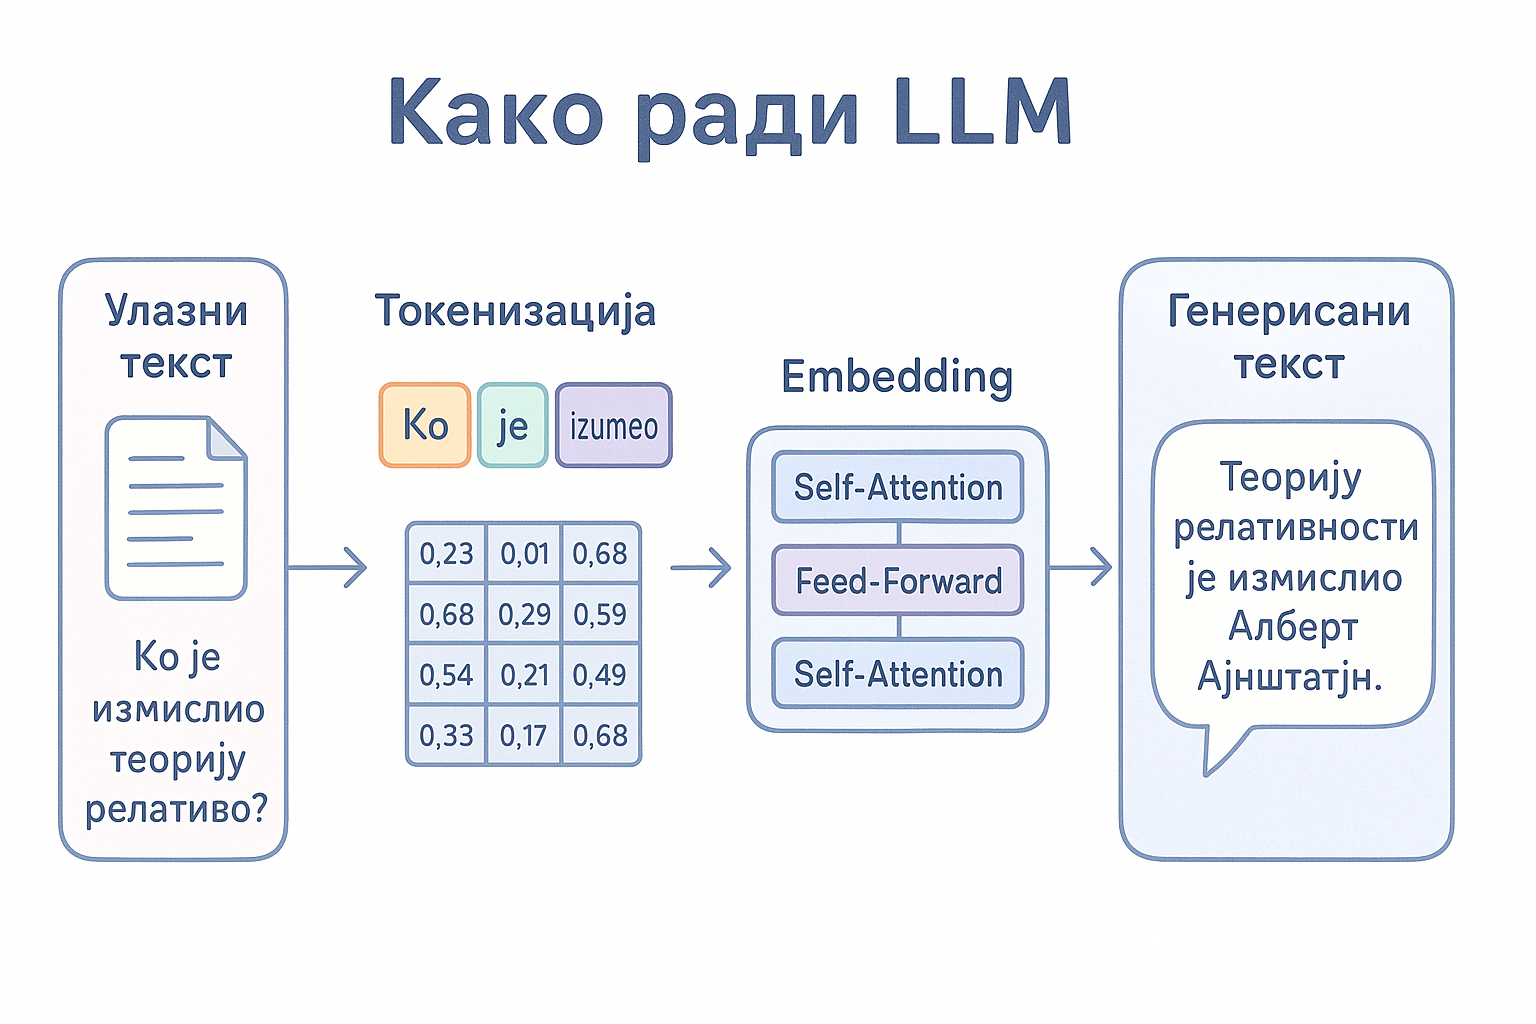
\includegraphics[width=0.8\textwidth]{slike/04/LLM_slikovito.png}
    \caption{Приказ рада LLM система}
    \label{fig:04-11}
\end{figure}
\noindent
Када у n8n-у пошаљете захтев ка OpenAI API-ју, ви заправо шаљете текст њиховом \textit{извршном фајлу} на серверу. Тај фајл консултује \textit{fajl sa parametrima} (GPT-4.1 модел), врши милионе математичких операција у милисекунди и враћа резултат. Разумевање ове поделе је важно јер објашњава зашто су јачи модели спорији и скупљи – они захтевају учитавање већих фајлова са параметрима и обављање више математичких операција за сваку генерисану реч.

\subsection{Механизам закључивања: Предикција наредног токена}

Једна од најчешћих заблуда у јавном дискурсу о вештачкој интелигенцији је антропоморфизација LLM-а – приписивање људских особина машини. Императив је разумети: Велики језички модел не поседује когнитивни апарат за разумевање текста, логике или истине. Он не зна чињенице на онтолошки начин на који их знају људи.
LLM је, у својој суштини, софистицирана статистичка машина за предвиђање (Auto-regressive Model). Његова једина функција је израчунавање вероватноће појављивања наредног симбола (токена) у низу, базирано искључиво на математичким обрасцима уоченим током тренинга на петабајтима текста.
Процес генерисања одговора није креативан чин, већ серија пробабилистичких калкулација које се одвијају секвенцијално, токен по токен.

\subsubsection{Студија случаја: Пробабилистичка дистрибуција}

Да бисмо илустровали овај механизам, анализираћемо једноставан лингвистички упит. Претпоставимо да моделу пошаљемо улазни промпт:
\begin{center}
\textit{"Ajfelov toranj se nalazi u..."}
\end{center}

У тренутку када модел прими овај низ, он не визуализује металну структуру у Паризу. Уместо тога, он врши следеће операције:
\begin{enumerate}
    \item \textbf{Анализа контекста:} Модел анализира токене Ајфелов, торањ, се, налази, у.
    \item \textbf{Претрага образаца:} Консултује своје интерне параметре (тежине) да види које речи су се у његовим тренинг подацима (књигама, википедији, чланцима) најчешће појављивале након ове специфичне секвенце.
    \item \textbf{Израчунавање вероватноће:} Модел додељује проценат вероватноће свакој речи у свом речнику (који може садржати преко 50.000 токена).
\end{enumerate}

Резултат ове операције је листа вероватноћа (дистрибуција):

\begin{itemize}
    \item \textbf{Паризу} $\rightarrow$ \textbf{97.4\%} (Висока семантичка и фактичка корелација у тренинг подацима).
    \item \textbf{Француској} $\rightarrow$ \textbf{2.1\%} (Граматички исправно, али се ређе користи у овом специфичном фразеолошком контексту).
    \item \textbf{центру} $\rightarrow$ \textbf{0.3\%} (Могућ наставак: "...центру Париза").
    \item \textbf{Лондону} $\rightarrow$ \textbf{0.001\%} (Статистичка аномалија или помињање у контексту поређења).
    \item \textbf{сендвичу} $\rightarrow$ \textbf{0.00001\%} (Потпуно одсуство семантичке везе).
\end{itemize}

Модел затим примењује алгоритам узорковања (Sampling) и бира токен са највишим скором – у овом случају Паризу.
Затим се тај нови токен додаје на крај реченице, и процес се понавља за следећу реч.

\textbf{Кључна импликација за инжењеринг:}
Овај механизам објашњава зашто модели могу да лажу самоуверено. Ако је модел трениран на хипотетичком скупу података где у 90\% текстова пише да је Ајфелов торањ у Берлину, модел би са високом вероватноћом предвидео Берлину. За модел, \textbf{истина није усклађеност са реалношћу, већ усклађеност са тренинг подацима.}
\subsubsection{Контрола креативности: Параметар Temperature}

У n8n чворовима за AI, често ћете видети поље \textbf{Temperature}. Ово је директна контрола над механизмом предвиђања који смо управо описали.

\begin{tcolorbox}[colback=blue!5!white,colframe=blue!75!black,title=Podešavanje Temperature]
\begin{itemize}
    \item \textbf{Ниска температура (0.0 - 0.3):} Модел је конзервативан. Увек бира реч са највећом вероватноћом.
    \textit{Koristiti za:} Екстракцију података, кодирање, фактуре, JSON излаз. Желимо прецизност, не изненађења.
    
    \item \textbf{Висока температура (0.7 - 1.0):} Модел постаје „креативан“. Понекад ће намерно изабрати реч са мањом вероватноћом да би текст звучао разноврсније.
    \textit{Koristiti za:} Писање блогова, маркетинг слогана, креативно писање.
\end{itemize}
\end{tcolorbox}

\subsection{Процес тренинга великих језичких модела}

Процес иницијалног тренинга великог језичког модела, познат као \textbf{pre-training}, представља фундаменталну фазу у настанку ових система и чини основу свих њихових каснијих способности. У овој фази модел се не тренира за конкретан задатак, домен или апликацију, већ стиче опште знање о језику, структури текста и обрасцима људске комуникације. Pre-training се може посматрати као процес у коме се неуронска мрежа излаже огромној количини текстуалних података како би научила статистичке и семантичке законитости које важе у природном језику.

Са инжењерског становишта, pre-training представља проблем оптимизације изузетно високих димензија. Савремени модели садрже десетине или стотине милијарди параметара, а сваки од тих параметара учествује у формирању излаза модела. Циљ тренинга је пронаћи такву конфигурацију параметара која минимизује укупну грешку на целокупном скупу података, односно која омогућава моделу да са што већом вероватноћом предвиди наредни елемент у секвенци текста.

\subsubsection{Формулација задатка: предикција наредног токена}

Основни тренинг задатак у pre-training фази своди се на проблем предикције наредног токена (енг. \textit{next-token prediction}). Текстуални улаз се најпре дели на мање јединице — токене — који могу представљати речи, делове речи, симболе или чак појединачне карактере. Модел добија секвенцу токена и у сваком кораку има задатак да процени вероватноћу сваког могућег наредног токена из унапред дефинисаног вокабулара.

Формално, модел учи апроксимацију условне вероватноће:

\[
P(t_{n+1} \mid t_1, t_2, \dots, t_n)
\]

где $t_i$ представљају токене у секвенци. Иако овај задатак на први поглед делује једноставно, његова последица је изузетно моћна: да би успешно предвидео наредни токен, модел мора имплицитно да разуме граматику, значење речи, контекст, стил писања, као и шире семантичке односе у тексту.

\subsubsection{Један тренинг корак и оптимизација}

Током тренинга, модел пролази кроз следећи циклус који се понавља огроман број пута:

Најпре се улазна секвенца токена пропагира унапред кроз неуронску мрежу (енг. \textit{forward pass}), при чему се на излазу добија дистрибуција вероватноћа над свим могућим наредним токенима. Затим се ова дистрибуција пореди са стварним токеном који се појављује у подацима. Разлика између предвиђене и стварне вредности мери се функцијом грешке, најчешће \textit{cross-entropy loss} функцијом.

Добијена грешка се потом пропагира уназад кроз мрежу (енг. \textit{backpropagation}), чиме се израчунава колико је сваки појединачни параметар допринео укупној грешци. На основу тог сигнала, параметри се коригују у веома малим корацима коришћењем варијанти градијентног спуста (нпр. алгоритми Adam или AdamW оптимизатора). Ове корекције су микроскопске, али се њихов ефекат акумулира кроз огроман број итерација.

Важно је истаћи да у овом процесу модел не добија експлицитне инструкције о значењу речи, правилима језика или логици. Све те способности се појављују као резултат статистичке оптимизације над великим бројем примера.

\subsubsection{Природа наученог знања}

Знање које модел стиче током pre-training фазе није експлицитно запамћено у облику база података или правила. Уместо тога, оно је имплицитно кодирано у тежинама неуронске мреже. То значи да се информације не могу једноставно „прочитати“ из модела, већ се испољавају кроз понашање модела током генерисања текста.

Овакав облик знања има неколико кључних карактеристика. Прво, оно је дистрибуирано — ниједан појединачни параметар не садржи одређену чињеницу, већ се информације појављују као резултат интеракције великог броја параметара. Друго, знање је апроксимативно и пробабилистичко, што објашњава зашто модели могу правити грешке или генерисати нетачне информације, али и зашто су способни за генерализацију на нове, невиђене примере.

Због тога се често каже да велики језички модели не „памте“ интернет, већ да га компресују у облику високо-димензионалног математичког простора. Ова компресија је са губитком (\textit{lossy}), слично као код JPEG компресије слике: задржавају се обрасци и структура, али не и сваки појединачни детаљ.

Један од најзанимљивијих аспеката pre-training фазе је појава тзв. специјалних способности. Како се величина модела и количина података повећавају, модел изненада почиње да показује понашања која нису била експлицитно тренирана, као што су основно резоновање, решавање математичких проблема, праћење инструкција или чак генерисање програмског кода.

Ове способности се не појављују линеарно са растом модела, већ често нагло, након преласка одређеног прага у броју параметара или количини података. Ово указује на то да pre-training не учи само локалне обрасце језика, већ гради апстрактне репрезентације које омогућавају сложеније облике когнитивног понашања.

\subsubsection{Ограничења pre-training фазе}

Иако је pre-training кључан за перформансе великих језичких модела, он има и своја ограничења. Модели тренирани искључиво на овом принципу немају експлицитно разумевање циљева корисника, етичких норми или контекста употребе. Такође, њихово знање је статично и ограничено временским периодом обухваћеним тренинг подацима.
Због тога се pre-training у пракси готово увек надопуњује додатним фазама, као што су fine-tuning на специфичним задацима, генерисање синтетичких инструкција (Self-Instruct)~\cite{wang2023selfinstruct} и усклађивање са људским преференцама (нпр. RLHF~\cite{ouyang2022,bai2022} или Direct Preference Optimization)~\cite{rafailov2023dpo}. Међутим, без снажне и обимне pre-training фазе, ове касније фазе не би имале стабилну основу на којој могу да граде додатне способности.
Pre-training представља темељ на којем почива целокупно понашање великих језичких модела. Он трансформише сирове текстуалне податке у општу језичку и семантичку компетенцију, омогућавајући моделима да функционишу као универзални алати за обраду и генерисање језика.

\subsection{Fine-Tuning: Специјализација и доменска адаптација}

Иако су велики језички модели тренирани на огромном корпусу општег знања, они су по својој природи генералисти. У специфичним инжењерским применама, често се јавља потреба да модел усвоји специфичан жаргон, формат излаза или стил комуникације који није био заступљен у иницијалном тренингу. Ту наступа процес финог подешавања (енг. \textit{Fine-Tuning})~\cite{ouyang2022,hu2022lora}.

Ако процес иницијалног тренинга (pre-training) посматрамо као стицање општег образовања, где модел учи синтаксу, логику и опште чињенице о свету, онда је fine-tuning еквивалентан специјалистичкој стручној обуци. Модел не учи како да говори, већ како да одговара у контексту специфичне организације или индустрије.

\subsubsection{Технички процес и примена}
Процес подразумева наставак тренинга модела на мањем, висококвалитетном скупу података, специфичном за домен примене. Овај метод спада у домен надгледаног учења (енг. \textit{Supervised Learning}), где се користе парови података у формату "Улаз $\rightarrow$ Жељени Излаз".

Кључни сценарији примене укључују:
\begin{itemize}
    \item \textbf{Стилска и тонална адаптација:} Тренирање модела на корпоративној архиви комуникације како би генерисани одговори рефлектовали специфичан начин генерисања одговора, терминологију и форматирање.
    \item \textbf{Структурална усклађеност:} Тренирање модела да конзистентно генерише излаз у специфичним, често нестандардним форматима (нпр. власнички XML шеме или специфични JSON формати), чиме се минимизира ризик од грешака при парсирању.
    \item \textbf{Оптимизација ресурса:} Мањи модел (нпр. 7 милијарди параметара) који је фино подешен за један специфичан задатак често може надмашити перформансе гигантског модела (GPT-4.1), уз драстично мање трошкове инференције и мању латенцију~\cite{chen2023frugal,hu2022lora}.
\end{itemize}

\begin{tcolorbox}[colback=green!5!white,colframe=green!75!black,title=Arhitektonska dilema: RAG ili Fine-Tuning?]
У пројектовању AI система, инжењери морају направити избор између две методологије побољшања перформанси:
\begin{itemize}
    \item \textbf{RAG (Retrieval-Augmented Generation):} Користи се када је потребно моделу пружити \textit{novo znanje} или променљиве чињенице (нпр. тренутно стање залиха, вести). RAG функционише као отворена књига током испита.
    \item \textbf{Fine-Tuning:} Користи се када је потребно променити \textit{понашање} модела или научити га новој \textit{вештини} (нпр. специфичан начин писања кода). Сликовито, fine-tuning мења синапсе у мозгу модела.
\end{itemize}
У пракси, најробуснији системи често користе хибридни приступ.
\end{tcolorbox}

На слици~\ref{fig:04-12} дат је илустративни приказ тренинга модела по свакој фази.


\begin{figure}[h!]
    \centering
    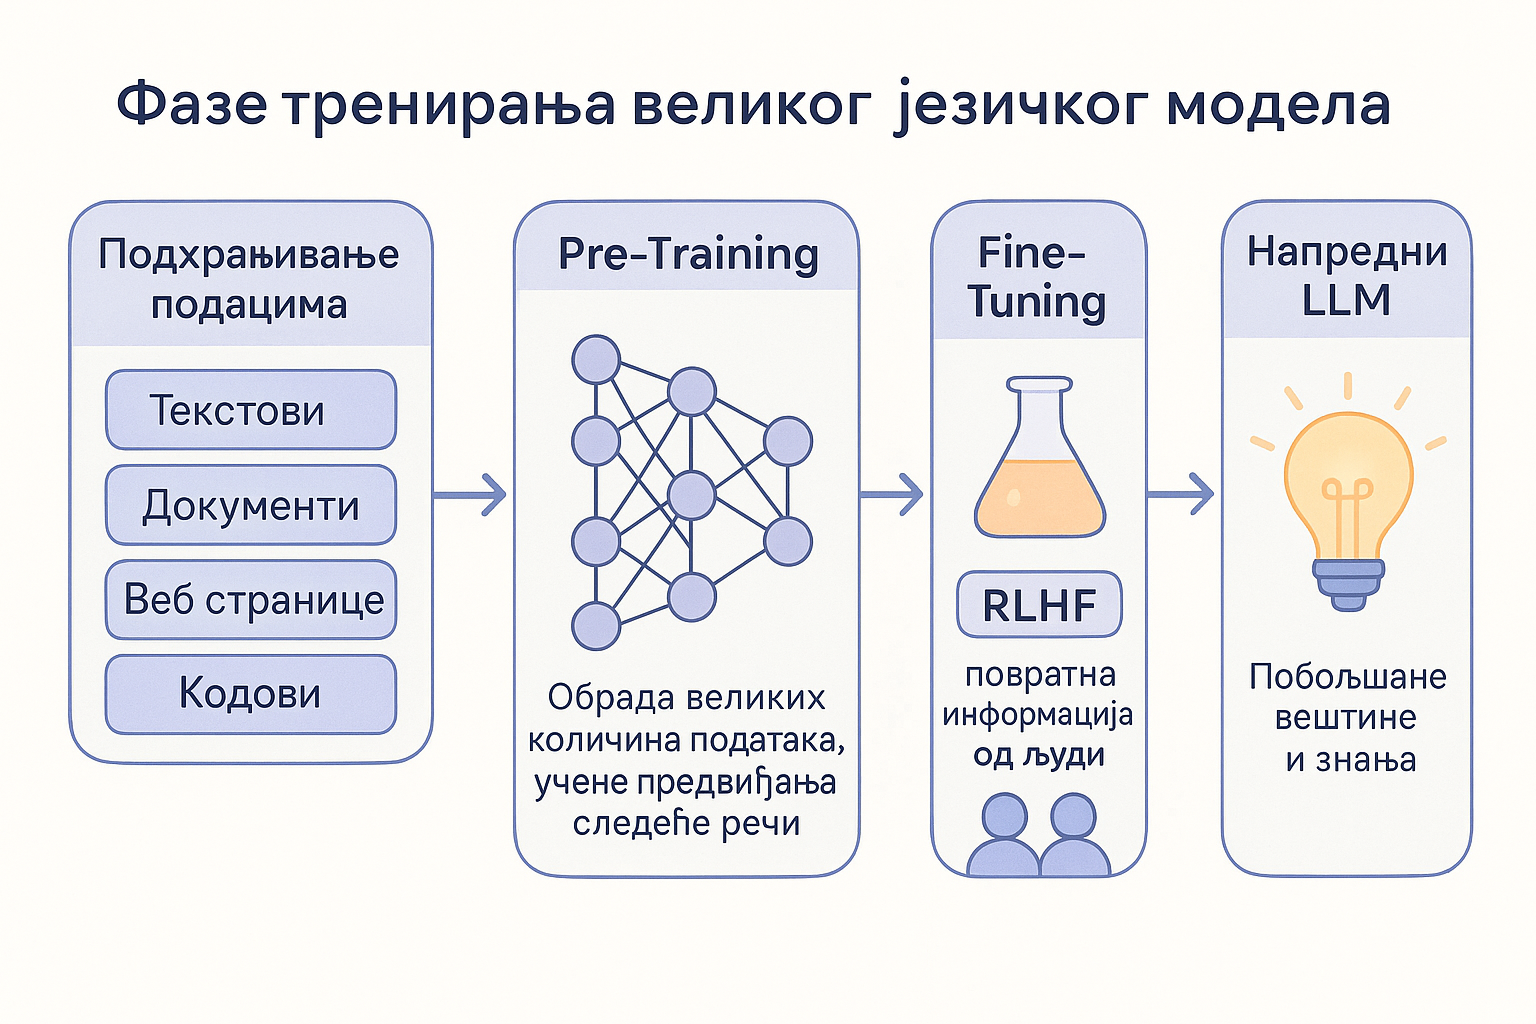
\includegraphics[width=0.95\textwidth]{slike/04/treniranje_modela.png}
    \caption{Илустрација процеса тренинга модела}
    \label{fig:04-12}
\end{figure}



\subsection{Трансформативна улога: Од генератора текста до Аутономног Агента}

Најзначајнија еволуција у примени LLM технологије огледа се у транзицији са парадигме пасивног \textit{AI Asistenata-a} на парадигму активног \textit{Agenta}.

Сами по себи, LLM-ови су изоловани системи за обраду текста, без директне везе са спољним светом. Међутим, када се интегришу у шире софтверске системе путем API интерфејса, они добијају способност перцепције и деловања.

\subsubsection{Механизам оперативног деловања}
Фундаментално питање гласи: \textit{Како пробабилистички модел, који само предвиђа наредну реч, може управљати детерминистичким софтверским системима?} Одговор лежи у механизму позивања функција (енг. \textit{Function Calling}) и генерисању структурираних података.

Процес доношења одлука у агентској архитектури одвија се кроз следеће фазе:

\begin{enumerate}
    \item \textbf{Детекција намере (енг. \textit{Intent Recognition}):} Корисник упућује захтев природним језиком (нпр. "Закажи састанак са клијентом Х за сутра у 10х").
    \item \textbf{Расудивање и формулација команде:} LLM анализира захтев и, уместо генерисања конверзацијског одговора, конструише структурирани објекат (најчешће у JSON формату) који представља инструкцију за екстерни систем.
    \\
    \begin{lstlisting}[language=json, basicstyle=\ttfamily\scriptsize, caption={Primer strukturirane instrukcije koju generiše Agent}]
    {
      "service": "calendar_api",
      "operation": "create_event",
      "payload": {
        "title": "Meeting with Client X",
        "datetime": "2024-10-25T10:00:00Z",
        "duration_minutes": 60,
        "attendees": ["client@example.com"]
      }
    }
    \end{lstlisting}
    
    \item \textbf{Извршење (Execution Runtime):} Контролни софтвер (бекенд систем) детектује овај структурирани излаз, валидира га и извршава стварни API позив ка циљном сервису (нпр. календару или бази података).
    \item \textbf{Повратна спрега (Feedback Loop):} Резултат извршења (успех или грешка) враћа се моделу као нови улазни податак. Модел затим генерише финални одговор кориснику („Састанак је успешно заказан“).
\end{enumerate}

У овој архитектури, LLM преузима улогу когнитивног контролера. Он не врши саму радњу (не шаље мрежне пакете), већ оркестрира алате. Његова функција је превођење нејасних, неструктурираних људских намера у прецизне, машински читљиве инструкције. Ово је суштина агентске технологије: премошћавање јаза између флексибилности људског језика и ригидности софтверских API-ја.

% =================================================================================
% POGLAVLJE 4
% =================================================================================

% =================================================================================
% POGLAVLJE 5
% =================================================================================

\section{Алати за развој аутоматизације: Платформа n8n}

У претходним поглављима разматрани су концептуални и архитектонски темељи
AI аутоматизације: референтна слојевита архитектура, таксономија AI система,
као и унутрашњи механизми великих језичких модела. Сада се фокус пребацује
са теоријских оквира на конкретан инжењерски алат кроз који се ови концепти
могу практично реализовати. За потребе овог курса, као репрезентативна
платформа за изградњу аутоматизованих и AI-оријентисаних радних токова
анализираће се платформа \textbf{n8n}.

n8n (чита се „ен–ејт–ен“, што се односи на скраћеницу појма
\textit{nodemation}, односно \textit{node-based automation})~\cite{n8n} развијена је
2019. године и представља један од најистакнутијих представника нове
генерације алата за визуелну оркестрацију процеса. За разлику од класичних
„low-code/no-code“ сервиса, који су углавном искључиво затворени и
хостовани у облаку, n8n се издваја комбинацијом отворености изворног
кода, могућности самосталног хостовања и нативне интеграције са
екосистемом великих језичких модела.

Разлози због којих се n8n користи као репрезентативна платформа у овом
курсу су тројаки:

\begin{itemize}
    \item \textbf{Репрезентативност:} n8n имплементира све кључне
    елементе референтне архитектуре из одељка~\ref{sec:tehnicka-infrastruktura} — тригере, оркестрацију,
    интеграције, податковни слој, AI слој и основни опсервациони слој.
    \item \textbf{Приступачност:} платформа је доступна бесплатно за
    самостално хостовање, што омогућава студентима и истраживачима
    експериментисање без финансијских баријера.
    \item \textbf{Едукативна транспарентност:} за разлику од потпуно
    затворених SaaS решења, код n8n-а су извршне инстанце, подаци и
    логови доступни инжењеру, што омогућава дубље разумевање рада
    аутоматизације.
\end{itemize}

Важно је нагласити да n8n у овом контексту није ексклузивни избор, већ
\textit{дидактички медиј}: принципи који се уче кроз n8n
(моделовање тока, рад са чворовима, експресије, AI интеграција)
директно су преносиви на друге платформе као што су Make (раније Интегромат),
Zapier, Microsoft Power Automate, Pipedream или Apache Airflow.

\subsection{Архитектура n8n платформе}

Са становишта софтверског инжењерства, n8n није монолитан алат,
већ скуп међусобно повезаних компоненти које заједно чине
платформу за извршавање аутоматизованих радних токова. Разумевање
унутрашње архитектуре неопходно је за правилно доношење одлука
о начину имплементације, скалабилности, безбедности и интеграције
са постојећом инфраструктуром организације.

\subsubsection{Филозофија дизајна и лиценцни модел}

n8n је развијен у складу са принципом \textbf{fair-code} лиценцирања,
прецизније под лиценцом \textit{Sustainable Use License}. Ова лиценца
представља хибридни модел између традиционалног отвореног кода и
комерцијалног софтвера, са следећим кључним карактеристикама:

\begin{itemize}
    \item Изворни код је јавно доступан, може се прегледати,
    модификовати и користити у некомерцијалне сврхе и интерне
    пословне потребе организације.
    \item Дистрибуција модификованих верзија као конкурентског
    производа није дозвољена, чиме се штите економски интереси
    матичне компаније.
    \item Корисници могу самостално хостовати платформу без плаћања
    лиценце, што је посебно значајно за организације са рестриктивним
    политикама заштите података.
\end{itemize}

Овакав модел омогућава баланс између транспарентности и одрживости
развоја платформе, чиме се избегава класична дилема између
искључиво отворених и искључиво комерцијалних решења.

\subsubsection{Технолошки стек}

Са техничке стране, n8n је развијен у програмском језику
\textbf{TypeScript} и извршава се у \textbf{Node.js} окружењу.
Овај избор има неколико важних последица:

\begin{itemize}
    \item \textbf{Асинхрони модел извршавања:} Node.js природно
    подржава асинхроне операције, што одговара природи аутоматизације
    где се највећи део времена троши на чекање одговора од екстерних
    сервиса (API позиви, базе података).
    \item \textbf{Богат екосистем пакета:} преко \textit{npm} репозиторијума,
    n8n може искористити хиљаде постојећих библиотека за рад са различитим
    протоколима и форматима.
    \item \textbf{Проширивост у JavaScript-у:} кориснички Code чворови
    пишу се у JavaScript-у (и опционо Python-у кроз \textit{Pyodide}
    рунтиме), што омогућава директно проширење функционалности без
    напуштања платформе.
\end{itemize}

Frontend (визуелни едитор) имплементиран је као Single-Page Application
заснована на \textit{Vue.js} оквиру, док је backend организован као
модуларна колекција сервиса одговорних за извршавање, перзистенцију
и аутентификацију.

\subsubsection{Модели имплементације}

n8n се може инсталирати и користити у неколико различитих модела,
од којих сваки има специфичне предности и ограничења:

\paragraph{n8n Cloud (Managed service)}
Комерцијална верзија у којој n8n тим управља целокупном инфраструктуром.
Корисник се пријављује, креира радне токове и не брине о серверима,
ажурирањима или резервним копијама. Овај модел је погодан за:
брзе прототипове, мање организације без DevOps капацитета и сценарије
где подаци нису строго поверљиви.

\paragraph{Self-hosted (Самостално хостовање)}
Најчешћи начин коришћења у академским и пословним окружењима.
n8n се дистрибуира као \textit{Docker} контејнер, што омогућава
једноставно покретање на било којој инфраструктури која подржава
контејнере. Типично размештање обухвата:

\begin{itemize}
    \item n8n апликацијски сервер (Node.js процес),
    \item перзистентну базу података (\textit{SQLite} за развој,
    \textit{PostgreSQL} или \textit{MySQL} за продукцију),
    \item опционално \textit{Redis} за queue мод (скалирано извршавање),
    \item reverse proxy (\textit{nginx}, \textit{Traefik}) за HTTPS
    терминацију и webhook рутирање.
\end{itemize}

\paragraph{Embedded (Угњеждено)}
n8n се може интегрисати и као библиотека у оквиру других апликација,
чиме постаје уграђени мотор за аутоматизацију. Овај модел је релативно
редак и користи се у специјализованим производима који желе да својим
корисницима понуде визуелну изградњу токова без развоја сопственог
система од нуле.

\subsubsection{Главне компоненте система}

Без обзира на модел имплементације, интерна архитектура n8n-а
састоји се од неколико логички раздвојених компоненти:

\begin{enumerate}
    \item \textbf{Едитор UI:} визуелно окружење у којем корисник
    гради и визуализује радне токове. Представља слој презентације
    и не учествује директно у извршавању.
    \item \textbf{Workflow Engine:} централни мотор који интерпретира
    граф чворова, управља током података, редоследом извршавања
    и стањем тренутне инстанце.
    \item \textbf{Node Runtime:} извршно окружење за појединачне
    чворове. Сваки чвор је у суштини функција која прима улаз,
    обавља операцију и враћа излаз.
    \item \textbf{Persistence Layer:} слој базе података у којем се
    чувају дефиниције радних токова, креденцијали (енкриптовани),
    историја извршавања и конфигурација.
    \item \textbf{Webhook Server:} подсистем који прима долазне HTTP
    захтеве и покреће одговарајуће радне токове.
    \item \textbf{Scheduler:} интерни сервис за покретање радних
    токова према временском распореду.
    \item \textbf{Queue Worker (опционо):} у скалираним инсталацијама,
    извршавање радних токова се делегира посебним worker процесима
    који преузимају послове из Redis реда.
\end{enumerate}

\subsubsection{Позиционирање у односу на конкуренцију}

У категорији workflow аутоматион алата постоји неколико доминантних
платформи са којима се n8n најчешће пореди. Табела~\ref{tab:04-3}
приказује поједностављени компаративни преглед.

\begin{table}[h!]
\centering
\caption{Поређење n8n са сродним платформама за аутоматизацију}
\vspace{0.3cm}
\begin{adjustbox}{max width=\textwidth}
\begin{tabular}{|p{3.2cm}|p{2.7cm}|p{2.7cm}|p{2.7cm}|}
\hline
\textbf{Карактеристика} & \textbf{n8n} & \textbf{Zapier} & \textbf{Make} \\
\hline
Self-hosting & Да & Не & Не \\
\hline
Приступ изворном коду & Да (fair-code) & Не & Не \\
\hline
Ценовни модел & По извршавању радног тока & По задатку & По операцији \\
\hline
Code чворови & JavaScript / Python & Ограничено & JavaScript \\
\hline
Нативна AI интеграција & LangChain.js & Делимично & Делимично \\
\hline
Комплексне гранања & Напредније & Линеарније & Напредније \\
\hline
\end{tabular}
\end{adjustbox}
\label{tab:04-3}
\end{table}

Кључна предност n8n-а у поређењу са Zapier-ом јесте могућност
самосталног хостовања, док је у поређењу са Make платформом
n8n флексибилнији у смислу програмабилности и контроле над
извршним окружењем. Са друге стране, чисто визуелно искуство и
број готових интеграција често су зрелији код комерцијалних
конкурената.

\subsection{Структура радног тока (Workflow)}

Централни појам у n8n платформи јесте \textbf{радни ток}
(енг. \textit{workflow}). Са формалне стране, радни ток се може
описати као усмерени ациклични граф (енг. \textit{Directed Acyclic
Graph, DAG}), где:

\begin{itemize}
    \item \textbf{чворови} (\textit{nodes}) представљају појединачне
    операције (нпр. читање емаил-а, позив API-ја, трансформација
    података, позив LLM-а),
    \item \textbf{ивице} (\textit{connections}) представљају ток
    података између чворова,
    \item не сме постојати циклус у графу — ако је итеративно
    понашање потребно, оно се моделује кроз експлицитне Лооп или
    Суб-workflow конструкте.
\end{itemize}

Иако визуелно делује као дијаграм тока, n8n граф није чисто
контролни ток као у класичном програмирању, већ примарно
\textbf{ток података} (\textit{dataflow}) — свака веза преноси
структурисане податке из једног чвора у следећи.

\subsubsection{Податковни модел: рад са ставкама}

Једна од фундаменталних концептуалних разлика у односу на
традиционално програмирање јесте чињеница да n8n ради са
\textbf{низовима ставки} (енг. \textit{items}), а не са појединачним
вредностима. Свака ставка је JSON објекат облика:

\begin{lstlisting}[language=json, caption={Struktura stavke u n8n}]
{
  "json": {
    "id": 42,
    "email": "kupac@example.com",
    "iznos": 1500
  },
  "binary": { /* opcionalno: fajlovi, slike */ }
}
\end{lstlisting}

Када чвор прими 100 ставки као улаз, он се по подразумеваном
понашању извршава 100 пута — једном по свакој ставки. Овај
имплицитни „лооп“ је последица чињенице да се подаци у
аутоматизацији најчешће јављају у баженим облицима (листа
наруџбина, листа корисника, листа порука) и да се над сваком
ставком понавља иста операција.

Овакав податковни модел доноси неколико важних последица:

\begin{itemize}
    \item \textbf{Имплицитна паралелизација:} чвор не мора експлицитно
    да итерира кроз листу, већ се исти код аутоматски примењује на
    сваку ставку.
    \item \textbf{Хетерогеност ставки:} свака ставка може имати
    другачију структуру, што захтева пажљиво руковање када се
    очекује конзистентност.
    \item \textbf{Спајање и раздвајање токова:} помоћу чворова
    \textit{Merge} и \textit{Split In Batches} могуће је мењати
    грануларност обраде.
\end{itemize}

\subsubsection{Expressions и динамичке вредности}

Конфигурација чворова у n8n-у ретко је статичка. Најчешће се
вредности поља израчунавају динамички, на основу излаза претходних
чворова. За то служи систем \textbf{експресија} (\textit{expressions})
који користи поједностављени JavaScript синтаксни модел унутар
ознака \texttt{\{\{ \}\}}~\cite{n8n}.

Типични примери експресија:
\begin{itemize}
    \item \texttt{\{\{ \$json.email \}\}} — приступ пољу тренутне ставке,
    \item \texttt{\{\{ \$node["HTTP Request"].json.id \}\}} — приступ
    излазу конкретног претходног чвора,
    \item \texttt{\{\{ \$now.format("yyyy-MM-dd") \}\}} — коришћење
    помоћних функција (датуми, стрингови, бројеви),
    \item \texttt{\{\{ \$items().length \}\}} — агрегатне операције
    над целим низом ставки.
\end{itemize}

Expressions омогућавају да се логика писања кода замени
декларативним конфигурисањем, што значајно снижава праг уласка
за нетехничке кориснике, а истовремено задржава пуну флексибилност
за напредне сценарије.

\subsubsection{Типови чворова}

Са становишта архитектуре извршавања, чворови у n8n-у деле се
на три основне категорије:

\begin{enumerate}
    \item \textbf{Trigger чворови:} иницирају извршавање радног тока.
    Сваки workflow мора имати барем један триггер чвор.
    \item \textbf{Регулар (Action) чворови:} обављају операције
    над подацима — позиви API-ја, трансформације, логичке одлуке,
    писање у базу и слично.
    \item \textbf{Суб-workflow чворови:} омогућавају модуларност
    позивањем другог радног тока као функције, чиме се постиже
    декомпозиција сложених система.
\end{enumerate}

\subsection{Trigger чворови (Окидачи)}

Trigger чворови представљају улазну тачку сваког аутоматизованог
процеса. Њихова улога је да \textit{детектују догађај} и покрену
извршавање радног тока. У зависности од природе догађаја који
их активира, тригери се могу класификовати у неколико група.

\subsubsection{Мануални тригери}

Најједноставнији облик окидача, који се користи готово искључиво
током развоја и тестирања. Корисник експлицитно кликом у едитору
покреће извршавање. Мануални тригер нема механизам за покретање
у продукционом окружењу и служи превасходно као развојни алат.

\subsubsection{Временски тригери (Schedule / Cron)}

Временски тригери покрећу радни ток према унапред дефинисаном
распореду. Конфигурисање се врши или кроз поједностављени интерфејс
(нпр. „сваких 15 минута“, „сваког понедељка у 09:00“) или кроз
класичну \textit{cron} синтаксу за сложеније обрасце.

Типични сценарији употребе:
\begin{itemize}
    \item дневни извештаји у одређено време,
    \item периодична провера стања екстерних сервиса,
    \item batch обрада података током ноћи,
    \item слање подсетника корисницима.
\end{itemize}

\subsubsection{Webhook тригери}

Webhook тригери су HTTP ендпоинт-и које n8n експонира спољном
свету. Када екстерни систем пошаље HTTP захтев на тај ендпоинт,
радни ток се тренутно покреће. Овај модел омогућава реакцију у
реалном времену (латенција у милисекундама) и представља основу
за интеграцију са модерним SaaS апликацијама.

Разликујемо два мода webhook тригера:
\begin{itemize}
    \item \textbf{Синхрони мод:} клијент који је позвао webhook чека
    на одговор радног тока. Погодан када је резултат обраде неопходан
    позиваоцу (нпр. AI агент који враћа одговор кориснику).
    \item \textbf{Асинхрони мод:} радни ток одмах враћа потврду
    пријема, док се обрада наставља у позадини. Погодан за
    дуготрајне процесе где клијент не треба да чека.
\end{itemize}

\subsubsection{Polling и app-specific тригери}

Велика већина апликацијски-специфичних тригера (Gmail, Slack, Notion,
Google Drive и сл.) интерно функционише или кроз прави webhook
механизам (када га екстерна апликација подржава) или кроз
\textit{polling} — периодичну проверу стања кроз API. Иако је
polling технички мање ефикасан и уноси латенцију, он је често
једина опција за сервисе који не подржавају излазне webhook-е.

\subsection{Регулар (Action) чворови}

Регулар чворови чине највећи део сваког нетривијалног радног тока.
Они се могу груписати у неколико логичких категорија према својој
улози.

\subsubsection{Интеграциони чворови}

Највећи број n8n чворова представљају \textit{integracije} —
унапред упаковани конектори за конкретне сервисе (Gmail, Slack,
HubSpot, Salesforce, Notion, PostgreSQL итд.). Сваки интеграциони
чвор апстрахује детаље API комуникације и излаже кориснику
декларативан интерфејс за избор операција (нпр. „пошаљи поруку“,
„креирај запис“, „претражи контакте“).

Када готов конектор не постоји, користи се универзални
\textbf{HTTP Рекуест} чвор који омогућава директан позив било
ког REST или GraphQL API-ја. Ово практично значи да n8n може
комуницирати са апсолутно сваким системом који излаже неки облик
HTTP интерфејса.

\subsubsection{Логички чворови}

За управљање током извршавања користе се посебни логички
чворови:

\begin{itemize}
    \item \textbf{IF:} бинарно гранање на основу услова
    (једнако, садржи, веће од и сл.).
    \item \textbf{Switch:} вишесмерно гранање са до четири или више
    излазних путања, на основу вредности поља.
    \item \textbf{Merge:} спајање више грана у једну, са различитим
    стратегијама (по индексу, по кључу, додавањем).
    \item \textbf{Loop / Split In Batches:} експлицитно итерирање
    кроз ставке у мањим групама, корисно за рад са великим скуповима
    података и за поштовање API рате-лимит-а.
    \item \textbf{Wait:} паузирање извршавања на одређено време или
    до наступања екстерног догађаја, што омогућава дуготрајне токове
    са „human-in-the-loop“ елементима.
\end{itemize}

\subsubsection{Чворови за трансформацију података}

Реални радни токови готово увек захтевају трансформацију података
између различитих система. За то служе специјализовани чворови:

\begin{itemize}
    \item \textbf{Set / Edit Fields:} додавање, брисање или
    преименовање поља на ставкама.
    \item \textbf{Code (JavaScript/Python):} писање произвољне
    логике када декларативни чворови нису довољни.
    \item \textbf{Aggregate:} груписање ставки по кључу и
    израчунавање агрегатних вредности.
    \item \textbf{Item Lists:} операције над низовима
    (сортирање, дедупликација, избор потскупа).
\end{itemize}

\subsection{AI интеграција: нативна подршка за LangChain}

Од 2023. године, n8n је увео нативну интеграцију са
\textit{LangChain.js} библиотеком~\cite{langchain}, чиме је платформа постала
један од првих визуелних алата са потпуним уградним оквиром
за изградњу AI агената. Ова интеграција није само додатак,
већ засебна категорија чворова означена као \textbf{AI Нодес}.

\subsubsection{Типови AI чворова}

LangChain интеграција у n8n организована је кроз неколико
специјализованих група чворова:

\begin{itemize}
    \item \textbf{AI Agent чвор:} централни извршни чвор који
    имплементира агентску петљу (Thought–Action–Observation),
    описану у одељку~\ref{sec:taksonomija-ai}. Агент прихвата кориснички промпт и
    аутономно одлучује које алате (Tool чворове) да позове.
    \item \textbf{Chat Model чворови:} апстракције за конкретне
    LLM провајдере — OpenAI, Anthropic, Google Gemini, Mistral,
    као и локалне моделе кроз \textit{Ollama} или \textit{LM Studio}.
    \item \textbf{Memory чворови:} имплементација краткорочне и
    дугорочне меморије агента — buffer меморија (последњих
    \textit{n} порука), summary меморија (сажетак конверзације),
    vector меморија (семантичко памћење).
    \item \textbf{Tool чворови:} алати које агент може позивати —
    Calculator, Wikipedia, HTTP Request, или било који други
    n8n чвор обучен у tool wrapper.
    \item \textbf{Vector Store чворови:} интеграција са векторским
    базама (\textit{Pinecone, Qdrant, Weaviate, Supabase, Postgres
    pgvector}) као основа RAG архитектуре.
    \item \textbf{Document Loader и Text Splitter чворови:}
    помоћни чворови за припрему докумената пре векторизације.
\end{itemize}

\subsubsection{Модуларност агентске архитектуре}

Посебност n8n приступа AI агентима јесте што су појединачне
компоненте архитектуре (модел, меморија, алати) моделоване као
\textit{посебни чворови} који се повезују на централни AI Агент
чвор преко специфичних улазних портова. Овај дизајн има неколико
последица:

\begin{itemize}
    \item Промена LLM провајдера (нпр. са OpenAI на Anthropic)
    своди се на замену једног чвора, без измене логике агента.
    \item Меморија и алати су експлицитни и видљиви у дијаграму,
    што значајно олакшава разумевање и дебуговање.
    \item Исти агент може се позивати из више различитих радних
    токова, чиме се постиже поновна употребљивост.
\end{itemize}

\subsection{Credentials систем и безбедност}

Комуникација са екстерним сервисима захтева аутентификацију, што
отвара питање безбедног складиштења креденцијала. n8n имплементира
наменски \textbf{Credentials} подсистем са следећим својствима:

\begin{itemize}
    \item Креденцијали се чувају у бази података у
    \textbf{енкриптованом облику}, коришћењем кључа који је
    конфигурисан на нивоу инстанце (\texttt{N8N\_ENCRYPTION\_KEY}).
    \item Подржани су стандардни механизми аутентификације:
    Basic Auth, API Key, Bearer Token, OAuth1, OAuth2, JWT и
    произвољни custom HTTP заглавља.
    \item Креденцијали се могу \textbf{делити између корисника и
    тимова}, са грануларном контролом приступа.
    \item Вредности креденцијала се не приказују у логовима и
    извршној историји, чиме се спречава њихово случајно откривање.
\end{itemize}

Раздвајање конфигурације радног тока од креденцијала омогућава
и преносивост: исти workflow може се пренети из развојног у
продукционо окружење уз коришћење различитих скупова креденцијала,
без измене саме логике тока.

\subsection{Error handling, debugging и observability}

Робустност аутоматизованог система не мери се само по његовој
способности да ради у идеалним условима, већ и по начину на који
се понаша у присуству грешака. n8n нуди неколико слојева механизама
за рад са грешкама.

\subsubsection{Политике руковања грешкама на нивоу чвора}

Сваки чвор може се конфигурисати са специфичном политиком у случају
грешке:

\begin{itemize}
    \item \textbf{Stop Workflow (подразумевано):} цео радни ток се
    зауставља, а извршавање се бележи као неуспешно.
    \item \textbf{Continue on Fail:} грешка се бележи, али се
    извршавање наставља кроз алтернативну путању.
    \item \textbf{Retry on Fail:} чвор се аутоматски поново извршава
    одређени број пута, са конфигурисаним размаком (експоненцијални
    backoff).
\end{itemize}

\subsubsection{Error workflow}

Поред политика на нивоу чвора, n8n омогућава дефинисање посебног
\textbf{Error Workflow}-а — специјалног радног тока који се
аутоматски покреће сваки пут када главни workflow падне. Типична
употреба укључује слање нотификације DevOps тиму, креирање
тикета у систему за праћење грешака и логовање у екстерни
опсервациони систем (нпр. \textit{Sentry, Datadog}).

\subsubsection{Execution history и debugging}

Свако извршавање радног тока бележи се у \textbf{execution history}
где се могу прегледати улази и излази сваког чвора, статус и трајање.
Овај механизам представља основни опсервациони слој n8n платформе и
од непроцењиве је вредности током развоја и дијагностике.

Додатно, едитор поседује мод \textit{step-by-step execution} који
омогућава извршавање радног тока један чвор по чвор, са прегледом
података у сваком тренутку — аналогно класичном дебуггер-у у IDE
окружењима.

\subsection{Скалабилност и deployment}

За озбиљније продукционе примене, n8n нуди тзв. \textbf{queue mode}
архитектуру која раздваја примарну инстанцу (која прима webhook-ове и
управља сцхедулером) од једног или више \textbf{worker} процеса
који извршавају радне токове~\cite{n8n}. Комуникација између компоненти одвија
се кроз \textit{Redis} ред послова.

Овај приступ доноси следеће предности:
\begin{itemize}
    \item \textbf{Хоризонтална скалабилност:} број worker процеса
    може се динамички повећавати у зависности од оптерећења.
    \item \textbf{Отпорност на отказе:} пад једног worker-а не
    блокира примање нових окидача; незавршени послови се
    редистрибуирају.
    \item \textbf{Изолација ресурса:} дуготрајни и ресурсно захтевни
    радни токови могу се извршавати на посебним worker групама
    без утицаја на латенцију осталих.
\end{itemize}

У Kubernetes окружењима, n8n се може разместити кроз званичне
Helm chart-ове, што омогућава интеграцију са стандардним алатима
за мониторинг, autoscaling и управљање конфигурацијом.

\subsection{Пример имплементације: Интелигентна обрада корисничких тикета}

Да би се илустровала интеракција свих описаних компоненти, у наставку
се разматра реалистичан пример аутоматизације процеса корисничке
подршке. Циљ система је да сваки долазни email корисничке подршке
буде анализиран, класификован и обрађен на начин који минимизује
људски рад за рутинске случајеве, док комплексне и хитне случајеве
ескалира људском оператеру.

\subsubsection{Функционална спецификација}

Систем треба да:
\begin{enumerate}
    \item региструје сваки нови емаил упућен на адресу
    \texttt{support@firma.com},
    \item утврди тему поруке (Рачуни, Техничка подршка, Општи упит),
    \item процени емоционални тон корисника (неутралан, фрустриран,
    разјарен),
    \item за рутинске упите генерише предлог одговора ослоњен на
    базу знања компаније,
    \item за хитне или негативне случајеве ескалира тикет менаџеру
    путем Slack нотификације,
    \item у свим случајевима упише резиме у CRM систем.
\end{enumerate}

\subsubsection{Архитектура радног тока}

Имплементација се састоји од следећих чворова, повезаних у јединствен
граф:

\begin{enumerate}
    \item \textbf{Trigger чвор (Gmail Trigger):} активира се на сваку
    нову поруку. Конфигурисан као polling са интервалом од једне
    минуте.

    \item \textbf{Set чвор:} нормализује структуру података,
    издвајајући само релевантна поља: пошиљаоца, наслов, тело
    поруке и време пријема.

    \item \textbf{AI Agent чвор (Класификатор):} повезан на OpenAI
    Chat Model и конфигурисан са системским промптом који налаже
    строго структурисан JSON излаз. Пример очекиваног одговора:

\begin{lstlisting}[language=json, caption={Strukturisan izlaz klasifikacionog agenta}]
{
  "kategorija": "Tehnicka podrska",
  "ton": "frustriran",
  "hitnost": 8,
  "kratak_opis": "Korisnik ne moze da se prijavi vec dva dana"
}
\end{lstlisting}

    \item \textbf{Switch чвор:} усмерава ток извршавања у зависности
    од категорије и хитности:
    \begin{itemize}
        \item ако је хитност $\geq 7$ или је тон „разјарен“ —
        грана А (ескалација),
        \item ако је категорија „Рачуни“ — грана Б (финансије),
        \item у супротном — грана Ц (рутински одговор).
    \end{itemize}

    \item \textbf{Грана А (Ескалација) — Slack чвор:} шаље форматирано
    упозорење у канал \texttt{\#support-urgent}, уз линк ка оригиналном
    емаил-у и сажетак ситуације.

    \item \textbf{Грана Б (Финансије) — Forward + CRM:} прослеђује
    поруку финансијском тиму и аутоматски креира напомену у CRM-у.

    \item \textbf{Грана Ц (Рутински одговор) — RAG агент:} додатни AI
    агент повезан на векторску базу знања генерише предлог одговора
    утемељен у званичној документацији компаније. Овај предлог се
    \textbf{не шаље аутоматски}, већ се креира као драфт у Gmail-у,
    са нотификацијом оператеру да прегледа и одобри садржај.

    \item \textbf{Завршни чвор (PostgreSQL):} у свим гранама, на крају
    се у CRM базу уписује запис о обрађеном тикету са резултатима
    класификације и предузетим акцијама.

    \item \textbf{Error Workflow:} у случају било каквог отказа —
    недоступност OpenAI API-ја, грешка у Slack аутентификацији или
    пад базе — покреће се резервни ток који обавештава DevOps тим
    и привремено чува неуспешне ставке за каснију ручну обраду.
\end{enumerate}

На слици~\ref{fig:04-13} приказан је визуелни дијаграм описаног
радног тока, са свим главним чворовима, гранама извршавања и резервним
Error Workflow током.

\begin{figure}[h!]
    \centering
    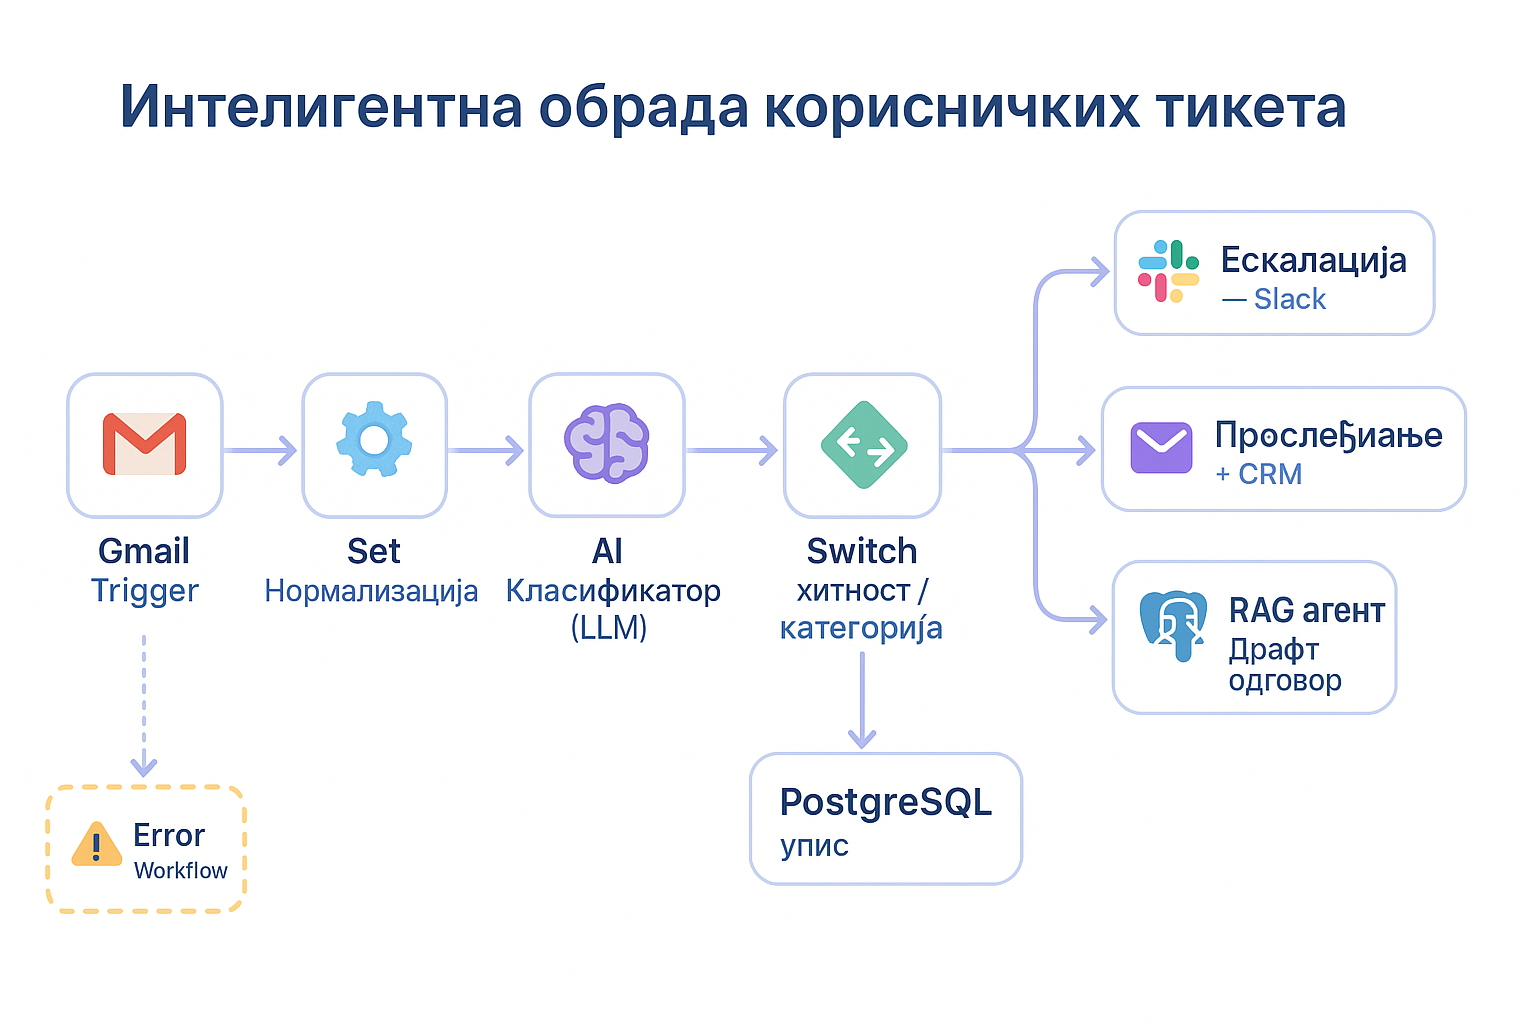
\includegraphics[width=0.95\textwidth]{slike/04/n8n_ticket_workflow.png}
    \caption{Визуелни приказ радног тока за интелигентну обраду корисничких тикета у \textit{n8n}}
    \label{fig:04-13}
\end{figure}

\subsubsection{Анализа решења}

Представљени пример демонстрира неколико кључних својстава
n8n платформе и општих принципа AI аутоматизације:

\begin{itemize}
    \item \textbf{Композитна интелигенција:} систем користи два
    независна AI агента — један за класификацију, други за
    генерисање одговора — што је у складу са принципом
    специјализације из мулти-агентске парадигме.
    \item \textbf{Структурисани излаз као интеграциона граница:}
    класификациони агент не враћа слободан текст, већ строго
    дефинисан JSON, што омогућава детерминистичко гранање у Switch
    чвору.
    \item \textbf{Human-in-the-loop:} за рутинске случајеве систем
    не преузима пуну одговорност, већ припрема предлог који човек
    одобрава — што је у складу са принципима Guardrails слоја из
    одељка~\ref{sec:tehnicka-infrastruktura}.
    \item \textbf{Отпорност на грешке:} експлицитно дефинисан Error
    Workflow обезбеђује да грешка у једном делу система не доведе
    до губитка корисничких упита.
    \item \textbf{Опсервабилност:} свака извршена инстанца радног
    тока оставља комплетан траг у execution history-ју, чиме се
    омогућава ревизија одлука и континуирано побољшање промптова
    и правила.
\end{itemize}

\subsubsection{Могући правци проширења}

Представљени систем може се постепено надограђивати увођењем
напреднијих компоненти:

\begin{itemize}
    \item додавањем дугорочне меморије агента, чиме систем
    „памти“ историју комуникације са сваким појединачним клијентом,
    \item увођењем евалуационог агента који вреднује квалитет
    генерисаних предлога и аутоматски усавршава промптове,
    \item проширењем на omnichannel сценарије (WhatsApp, web chat,
    позиви претворени у текст кроз STT моделе),
    \item интеграцијом са системом за аутоматску детекцију аномалија
    у оптерећењу и темама, што омогућава проактивно упозоравање
    менаџмента на системске проблеме.
\end{itemize}

Тиме се демонстрира како се релативно једноставан иницијални радни
ток може временом развијати у комплексан, аутономни систем за
подршку одлучивању, без фундаменталне промене основне архитектуре
платформе.

\newpage

% =================================================================================
% POGLAVLJE 6
% =================================================================================
\section{Будућност рада и етички аспекти}

Поред техничких аспеката AI система неопходно је сагледати шире импликације убрзаног развоја и примене AI система заснованих на агентима. Иако су претходна поглавља била фокусирана на техничке аспекте и архитектуралне разлике, стварни домет ове технологије огледа се у њеном утицају на економске структуре, тржиште рада, друштвене односе и етичке оквире доношења одлука. На слици~\ref{fig:04-14} дат је концептуални приказ кључних оса одговорног увођења AI система у радно окружење, као и трансформације улоге човека из непосредног извршиоца у надзорника и архитекту аутономних система.

\begin{figure}[h!]
    \centering
    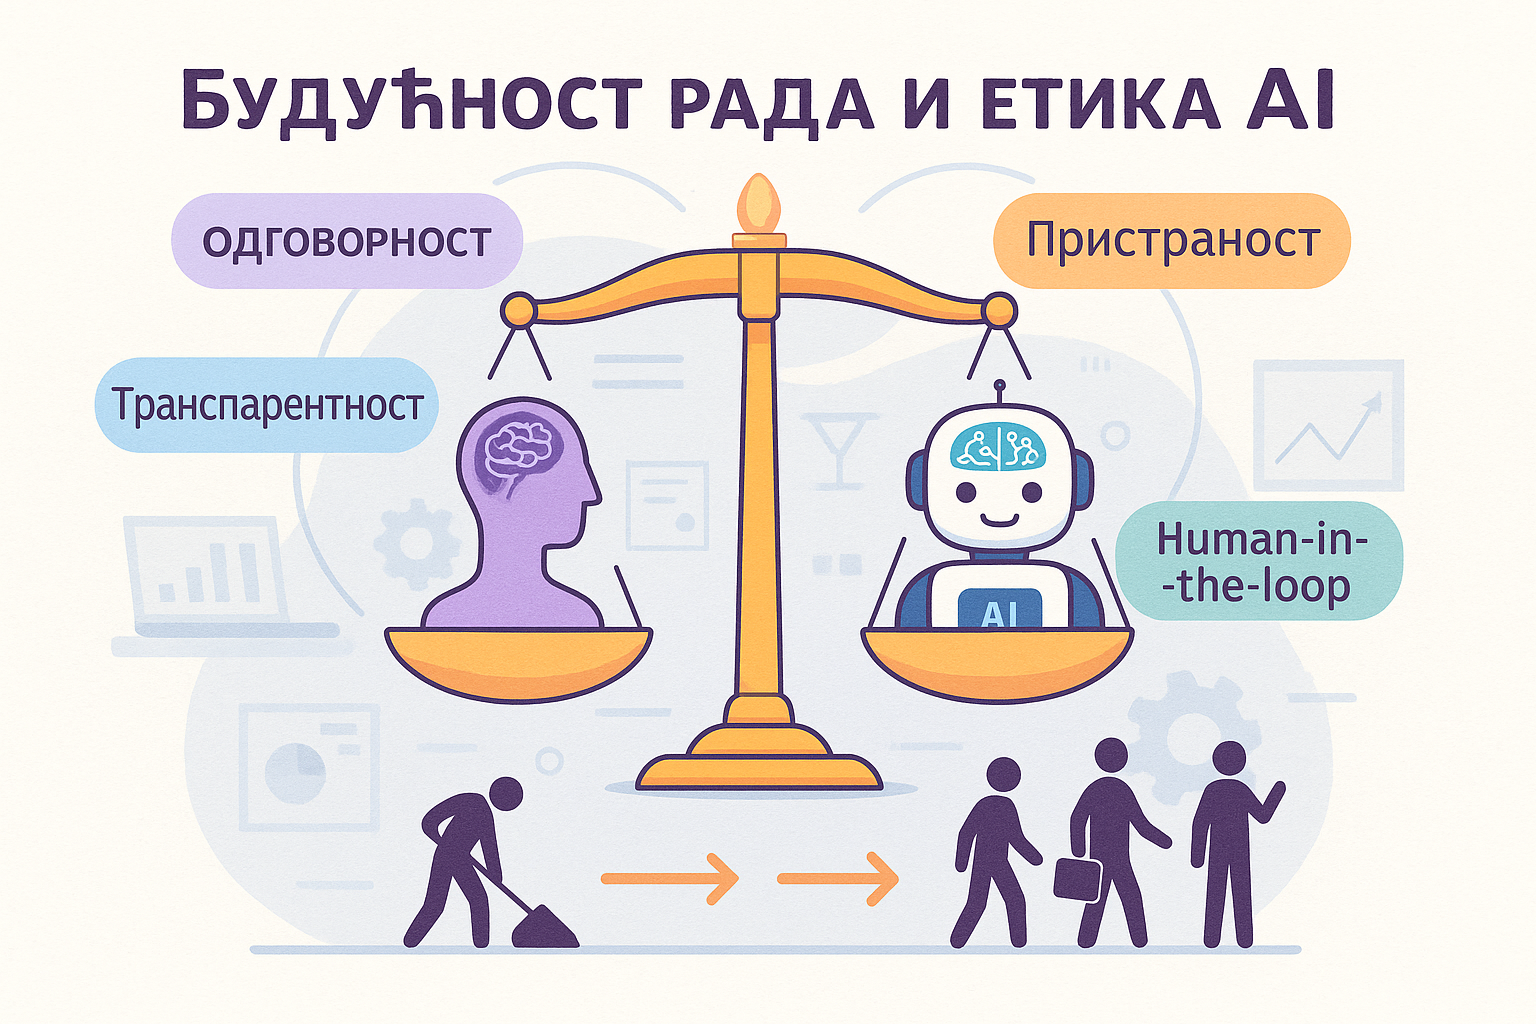
\includegraphics[width=0.85\textwidth]{slike/04/etika_buducnost_rada.png}
    \caption{Етички оквир и трансформација улоге човека у ери AI агената}
    \label{fig:04-14}
\end{figure}

Развој аутономних и полуаутономних AI агената не представља само технолошки напредак, већ и дубоку промену парадигме рада и организације друштва~\cite{schwab2017,frey2017}. У том контексту, AI се више не посматра искључиво као алат, већ као активни учесник у производњи вредности, доношењу одлука и управљању процесима.

\subsection{Економска предвиђања и продуктивност}

Један од најчешће истицаних макроекономских ефеката примене AI агената јесте драстичан раст индивидуалне продуктивности. Аутономни системи омогућавају да мали тимови, па чак и појединци, управљају процесима који су до недавно захтевали комплексне хијерархије, вишеслојне организационе структуре и значајне људске ресурсе.

AI агенти преузимају улоге аналитичара, оператера, планера и извршилаца, чиме се смањују трансакциони трошкови, убрзава доношење одлука и повећава брзина иновација. Овакав модел рада отвара простор за појаву изузетно агилних организација са минималним бројем запослених, али са диспропорционално великим економским утицајем.

Међутим, овакав раст продуктивности носи и ризике. Економска вредност се све више концентрише око власника технологије, података и инфраструктуре, што може довести до продубљивања неједнакости између различитих друштвених група, региона и држава. У одсуству адекватних регулаторних и редистрибутивних механизама, користи од AI револуције могу остати ограничене на узак слој актера.

\subsection{Трансформација тржишта рада}

Аутоматизација заснована на AI агентима неминовно доводи до трансформације структуре тржишта рада~\cite{frey2017,schwab2017}. Традиционална радна места, заснована на понављајућим, процедуралним или административним задацима, постају посебно рањива. Истовремено, не долази до потпуног нестанка људског рада, већ до његове дубоке реконфигурације.

Улога човека се постепено помера са директног извршавања задатака ка:
\begin{itemize}
    \item надзору аутономних система,
    \item дефинисању циљева и ограничења,
    \item евалуацији квалитета и последица одлука,
    \item управљању изузетним ситуацијама и грешкама.
\end{itemize}

Другим речима, човек постаје \textit{arhitekta sistema} и \textit{чувар смисла}, док AI преузима оперативни део рада. Ова промена захтева нове компетенције и континуирано прилагођавање образовних система.

Појављују се нове професионалне улоге и вештине:
\begin{itemize}
    \item \textbf{Промпт инжењеринг:} способност прецизног формулисања захтева, ограничења и циљева за AI системе~\cite{sahoo2024prompt};
    \item \textbf{Оркестрација агената:} дизајнирање и управљање интеракцијама између више аутономних агената у комплексним токовима рада;
    \item \textbf{AI надзор и евалуација:} процена поузданости, робусности и граница аутономних система;
    \item \textbf{Интердисциплинарна писменост:} разумевање како техничких, тако и друштвених и правних импликација AI одлука.
\end{itemize}

Истовремено, постоји реална опасност од структурне незапослености у секторима који не успеју да се прилагоде овом прелазу, што додатно наглашава потребу за активним политикама преквалификације и социјалне заштите.

\subsection{Етички аспекти аутономних AI система}

Са порастом аутономије AI агената, етичка питања постају централна тема њихове примене~\cite{hleg2019,bender2021}. Кључни изазов лежи у чињеници да AI системи доносе одлуке које могу имати директне последице по појединце и друштво, често на основу пробабилистичких и нетранспарентних модела~\cite{russell2020}.

Једно од основних етичких питања односи се на одговорност. У ситуацијама када AI агент направи грешку или проузрокује штету, поставља се питање: ко сноси одговорност — дизајнер система, корисник, организација или сам систем као аутономни ентитет? Тренутни правни оквири углавном нису прилагођени оваквим сценаријима.

Други кључни аспект је пристрасност~\cite{bender2021}. AI системи уче из података који рефлектују постојеће друштвене неједнакости, што може довести до репродукције или чак амплификације дискриминаторних образаца. Без континуираног етичког надзора, аутономни агенти могу доносити систематски неправедне одлуке, нарочито у областима као што су запошљавање, кредитирање или правосуђе~\cite{hleg2019}.

Трећи изазов представља транспарентност и објашњивост. Како системи постају сложенији и дистрибуиранији (посебно у мулти-агентским архитектурама), све је теже реконструисати ланац одлука који је довео до одређеног исхода. Ово отежава ревизију, регулацију и изградњу поверења између људи и AI система.

На дужи рок, широка примена AI агената може довести до редефинисања основних друштвених категорија рада, вредности и идентитета. Ако продуктивност постане готово независна од људског рада, друштва ће се суочити са питањима прерасподеле богатства, редефинисања радног времена и саме сврхе рада у људском животу.

Поставља се и питање когнитивне зависности: ослањање на AI агенте за планирање, доношење одлука и решавање проблема може довести до ерозије одређених људских вештина. Из тог разлога, будући системи морају бити дизајнирани не само као замена за људски рад, већ и као алат за његово унапређење.

Закључно, будућност рада у ери AI агената не зависи искључиво од технолошког напретка, већ од начина на који друштво одлучи да ову технологију интегрише. Баланс између ефикасности, праведности и људске аутономије представљаће један од кључних изазова савременог доба.

Важно је напоменути да AI аутоматизација није само технолошки тренд, већ фундаментална промена у начину организације рада. Прелазак са линеарних скрипти на аутономне агенте омогућава ниво продуктивности и скалабилности који је раније био незамислив.



% =================================================================================
% PRILOG
% =================================================================================

\section{Литература}
\printbibliography[heading=none]


\backmatter

\end{document}
